\documentclass[twoside]{book}

% Packages required by doxygen
\usepackage{fixltx2e}
\usepackage{calc}
\usepackage{doxygen}
\usepackage[export]{adjustbox} % also loads graphicx
\usepackage{graphicx}
\usepackage[utf8]{inputenc}
\usepackage{makeidx}
\usepackage{multicol}
\usepackage{multirow}
\PassOptionsToPackage{warn}{textcomp}
\usepackage{textcomp}
\usepackage[nointegrals]{wasysym}
\usepackage[table]{xcolor}

% Font selection
\usepackage[T1]{fontenc}
\usepackage[scaled=.90]{helvet}
\usepackage{courier}
\usepackage{amssymb}
\usepackage{sectsty}
\renewcommand{\familydefault}{\sfdefault}
\allsectionsfont{%
  \fontseries{bc}\selectfont%
  \color{darkgray}%
}
\renewcommand{\DoxyLabelFont}{%
  \fontseries{bc}\selectfont%
  \color{darkgray}%
}
\newcommand{\+}{\discretionary{\mbox{\scriptsize$\hookleftarrow$}}{}{}}

% Page & text layout
\usepackage{geometry}
\geometry{%
  a4paper,%
  top=2.5cm,%
  bottom=2.5cm,%
  left=2.5cm,%
  right=2.5cm%
}
\tolerance=750
\hfuzz=15pt
\hbadness=750
\setlength{\emergencystretch}{15pt}
\setlength{\parindent}{0cm}
\setlength{\parskip}{0.2cm}
\makeatletter
\renewcommand{\paragraph}{%
  \@startsection{paragraph}{4}{0ex}{-1.0ex}{1.0ex}{%
    \normalfont\normalsize\bfseries\SS@parafont%
  }%
}
\renewcommand{\subparagraph}{%
  \@startsection{subparagraph}{5}{0ex}{-1.0ex}{1.0ex}{%
    \normalfont\normalsize\bfseries\SS@subparafont%
  }%
}
\makeatother

% Headers & footers
\usepackage{fancyhdr}
\pagestyle{fancyplain}
\fancyhead[LE]{\fancyplain{}{\bfseries\thepage}}
\fancyhead[CE]{\fancyplain{}{}}
\fancyhead[RE]{\fancyplain{}{\bfseries\leftmark}}
\fancyhead[LO]{\fancyplain{}{\bfseries\rightmark}}
\fancyhead[CO]{\fancyplain{}{}}
\fancyhead[RO]{\fancyplain{}{\bfseries\thepage}}
\fancyfoot[LE]{\fancyplain{}{}}
\fancyfoot[CE]{\fancyplain{}{}}
\fancyfoot[RE]{\fancyplain{}{\bfseries\scriptsize Generated on Sun Jun 7 2015 21\+:40\+:32 for G\+U\+Inity by Doxygen }}
\fancyfoot[LO]{\fancyplain{}{\bfseries\scriptsize Generated on Sun Jun 7 2015 21\+:40\+:32 for G\+U\+Inity by Doxygen }}
\fancyfoot[CO]{\fancyplain{}{}}
\fancyfoot[RO]{\fancyplain{}{}}
\renewcommand{\footrulewidth}{0.4pt}
\renewcommand{\chaptermark}[1]{%
  \markboth{#1}{}%
}
\renewcommand{\sectionmark}[1]{%
  \markright{\thesection\ #1}%
}

% Indices & bibliography
\usepackage{natbib}
\usepackage[titles]{tocloft}
\setcounter{tocdepth}{3}
\setcounter{secnumdepth}{5}
\makeindex

% Hyperlinks (required, but should be loaded last)
\usepackage{ifpdf}
\ifpdf
  \usepackage[pdftex,pagebackref=true]{hyperref}
\else
  \usepackage[ps2pdf,pagebackref=true]{hyperref}
\fi
\hypersetup{%
  colorlinks=true,%
  linkcolor=blue,%
  citecolor=blue,%
  unicode%
}

% Custom commands
\newcommand{\clearemptydoublepage}{%
  \newpage{\pagestyle{empty}\cleardoublepage}%
}


%===== C O N T E N T S =====

\begin{document}

% Titlepage & ToC
\hypersetup{pageanchor=false,
             bookmarks=true,
             bookmarksnumbered=true,
             pdfencoding=unicode
            }
\pagenumbering{roman}
\begin{titlepage}
\vspace*{7cm}
\begin{center}%
{\Large G\+U\+Inity }\\
\vspace*{1cm}
{\large Generated by Doxygen 1.8.9.1}\\
\vspace*{0.5cm}
{\small Sun Jun 7 2015 21:40:32}\\
\end{center}
\end{titlepage}
\clearemptydoublepage
\tableofcontents
\clearemptydoublepage
\pagenumbering{arabic}
\hypersetup{pageanchor=true}

%--- Begin generated contents ---
\chapter{Module Index}
\section{Modules}
Here is a list of all modules\+:\begin{DoxyCompactList}
\item \contentsline{section}{Serialization Functions}{\pageref{group__serialization__functions}}{}
\end{DoxyCompactList}

\chapter{Hierarchical Index}
\section{Class Hierarchy}
This inheritance list is sorted roughly, but not completely, alphabetically\+:\begin{DoxyCompactList}
\item \contentsline{section}{Actor\+Description}{\pageref{struct_actor_description}}{}
\item \contentsline{section}{any\+\_\+type}{\pageref{classany__type}}{}
\begin{DoxyCompactList}
\item \contentsline{section}{concrete\+\_\+type$<$ T $>$}{\pageref{classconcrete__type}}{}
\end{DoxyCompactList}
\item \contentsline{section}{Asset}{\pageref{class_asset}}{}
\begin{DoxyCompactList}
\item \contentsline{section}{Font}{\pageref{class_font}}{}
\item \contentsline{section}{Material}{\pageref{class_material}}{}
\item \contentsline{section}{Mesh}{\pageref{class_mesh}}{}
\begin{DoxyCompactList}
\item \contentsline{section}{Skinned\+Mesh}{\pageref{class_skinned_mesh}}{}
\end{DoxyCompactList}
\item \contentsline{section}{Physics\+Material}{\pageref{class_physics_material}}{}
\item \contentsline{section}{Shader}{\pageref{class_shader}}{}
\item \contentsline{section}{Sound}{\pageref{class_sound}}{}
\item \contentsline{section}{Texture}{\pageref{class_texture}}{}
\end{DoxyCompactList}
\item \contentsline{section}{Asset\+Database}{\pageref{class_asset_database}}{}
\item \contentsline{section}{Component\+Description}{\pageref{class_component_description}}{}
\begin{DoxyCompactList}
\item \contentsline{section}{Camera\+Description}{\pageref{class_camera_description}}{}
\item \contentsline{section}{Collider\+Description}{\pageref{class_collider_description}}{}
\begin{DoxyCompactList}
\item \contentsline{section}{Box\+Collider\+Description}{\pageref{class_box_collider_description}}{}
\item \contentsline{section}{Capsule\+Collider\+Description}{\pageref{class_capsule_collider_description}}{}
\item \contentsline{section}{Sphere\+Collider\+Description}{\pageref{class_sphere_collider_description}}{}
\end{DoxyCompactList}
\item \contentsline{section}{Light\+Description}{\pageref{class_light_description}}{}
\item \contentsline{section}{Mesh\+Filter\+Description}{\pageref{class_mesh_filter_description}}{}
\item \contentsline{section}{Mesh\+Renderer\+Description}{\pageref{class_mesh_renderer_description}}{}
\item \contentsline{section}{Rigid\+Body\+Description}{\pageref{class_rigid_body_description}}{}
\item \contentsline{section}{Rigid\+Static\+Description}{\pageref{class_rigid_static_description}}{}
\end{DoxyCompactList}
\item enable\+\_\+shared\+\_\+from\+\_\+this\begin{DoxyCompactList}
\item \contentsline{section}{Actor}{\pageref{class_actor}}{}
\item \contentsline{section}{Component}{\pageref{class_component}}{}
\begin{DoxyCompactList}
\item \contentsline{section}{Camera}{\pageref{class_camera}}{}
\item \contentsline{section}{Collider}{\pageref{class_collider}}{}
\begin{DoxyCompactList}
\item \contentsline{section}{Box\+Collider}{\pageref{class_box_collider}}{}
\item \contentsline{section}{Capsule\+Collider}{\pageref{class_capsule_collider}}{}
\item \contentsline{section}{Mesh\+Collider}{\pageref{class_mesh_collider}}{}
\item \contentsline{section}{Sphere\+Collider}{\pageref{class_sphere_collider}}{}
\end{DoxyCompactList}
\item \contentsline{section}{Editor\+Collider}{\pageref{class_editor_collider}}{}
\item \contentsline{section}{Light}{\pageref{class_light}}{}
\item \contentsline{section}{Mesh\+Component}{\pageref{class_mesh_component}}{}
\begin{DoxyCompactList}
\item \contentsline{section}{Font\+Mesh}{\pageref{class_font_mesh}}{}
\item \contentsline{section}{Mesh\+Filter}{\pageref{class_mesh_filter}}{}
\end{DoxyCompactList}
\item \contentsline{section}{Mesh\+Renderer}{\pageref{class_mesh_renderer}}{}
\item \contentsline{section}{Rigid\+Body}{\pageref{class_rigid_body}}{}
\item \contentsline{section}{Rigid\+Static}{\pageref{class_rigid_static}}{}
\item \contentsline{section}{Script\+Component}{\pageref{class_script_component}}{}
\begin{DoxyCompactList}
\item \contentsline{section}{Add\+Force\+Script}{\pageref{class_add_force_script}}{}
\item \contentsline{section}{Editor\+Camera\+Control}{\pageref{class_editor_camera_control}}{}
\item \contentsline{section}{Increase\+Collider\+Script}{\pageref{class_increase_collider_script}}{}
\item \contentsline{section}{Move\+Handle}{\pageref{class_move_handle}}{}
\item \contentsline{section}{Move\+Tool}{\pageref{class_move_tool}}{}
\item \contentsline{section}{Player\+Script}{\pageref{class_player_script}}{}
\item \contentsline{section}{Rotate\+Handle}{\pageref{class_rotate_handle}}{}
\item \contentsline{section}{Rotate\+Over\+Time}{\pageref{class_rotate_over_time}}{}
\item \contentsline{section}{Rotate\+Tool}{\pageref{class_rotate_tool}}{}
\item \contentsline{section}{Scale\+Handle}{\pageref{class_scale_handle}}{}
\item \contentsline{section}{Scale\+Tool}{\pageref{class_scale_tool}}{}
\end{DoxyCompactList}
\end{DoxyCompactList}
\item \contentsline{section}{Editor}{\pageref{class_editor}}{}
\item \contentsline{section}{Game}{\pageref{class_game}}{}
\item \contentsline{section}{Transform}{\pageref{class_transform}}{}
\item \contentsline{section}{World}{\pageref{class_world}}{}
\end{DoxyCompactList}
\item \contentsline{section}{Graphics\+System}{\pageref{class_graphics_system}}{}
\begin{DoxyCompactList}
\item \contentsline{section}{G\+L\+F\+W\+Graphics\+System}{\pageref{class_g_l_f_w_graphics_system}}{}
\end{DoxyCompactList}
\item \contentsline{section}{Holder}{\pageref{class_holder}}{}
\item \contentsline{section}{Input}{\pageref{class_input}}{}
\item \contentsline{section}{Letter\+Font\+U\+V}{\pageref{struct_letter_font_u_v}}{}
\item \contentsline{section}{Member\+Info}{\pageref{struct_member_info}}{}
\item \contentsline{section}{Mesh\+Importer}{\pageref{class_mesh_importer}}{}
\item \contentsline{section}{Mesh\+Vertex}{\pageref{struct_mesh_vertex}}{}
\item \contentsline{section}{Observer}{\pageref{class_observer}}{}
\begin{DoxyCompactList}
\item \contentsline{section}{World}{\pageref{class_world}}{}
\end{DoxyCompactList}
\item \contentsline{section}{Packed\+F\+B\+X\+Vertex}{\pageref{struct_packed_f_b_x_vertex}}{}
\item \contentsline{section}{Packed\+O\+B\+J\+Vertex}{\pageref{struct_packed_o_b_j_vertex}}{}
\item \contentsline{section}{Person}{\pageref{class_person}}{}
\item \contentsline{section}{Physics}{\pageref{class_physics}}{}
\item \contentsline{section}{Plane}{\pageref{struct_plane}}{}
\item \contentsline{section}{Pointer\+Holder$<$ T $>$}{\pageref{class_pointer_holder}}{}
\item Px\+Allocator\+Callback\begin{DoxyCompactList}
\item \contentsline{section}{Phys\+X\+Allocator\+Callback}{\pageref{class_phys_x_allocator_callback}}{}
\end{DoxyCompactList}
\item Px\+Physics\+Insertion\+Callback\begin{DoxyCompactList}
\item \contentsline{section}{Phys\+X\+Insertion\+Callback}{\pageref{class_phys_x_insertion_callback}}{}
\end{DoxyCompactList}
\item Px\+Simulation\+Event\+Callback\begin{DoxyCompactList}
\item \contentsline{section}{Phys\+X\+Event\+Callback}{\pageref{class_phys_x_event_callback}}{}
\end{DoxyCompactList}
\item \contentsline{section}{Ray}{\pageref{class_ray}}{}
\item \contentsline{section}{Sound\+System}{\pageref{class_sound_system}}{}
\item \contentsline{section}{Spline}{\pageref{class_spline}}{}
\item \contentsline{section}{Static\+Counter$<$ T $>$}{\pageref{class_static_counter}}{}
\item \contentsline{section}{Subject$<$ T $>$}{\pageref{class_subject}}{}
\item \contentsline{section}{Subject$<$ Camera $>$}{\pageref{class_subject}}{}
\begin{DoxyCompactList}
\item \contentsline{section}{Camera}{\pageref{class_camera}}{}
\end{DoxyCompactList}
\item \contentsline{section}{Subject$<$ Editor\+Collider $>$}{\pageref{class_subject}}{}
\begin{DoxyCompactList}
\item \contentsline{section}{Editor\+Collider}{\pageref{class_editor_collider}}{}
\end{DoxyCompactList}
\item \contentsline{section}{Subject$<$ Factory $>$}{\pageref{class_subject}}{}
\begin{DoxyCompactList}
\item \contentsline{section}{Factory}{\pageref{class_factory}}{}
\end{DoxyCompactList}
\item \contentsline{section}{Subject$<$ Light $>$}{\pageref{class_subject}}{}
\begin{DoxyCompactList}
\item \contentsline{section}{Light}{\pageref{class_light}}{}
\end{DoxyCompactList}
\item \contentsline{section}{Subject$<$ Mesh\+Renderer $>$}{\pageref{class_subject}}{}
\begin{DoxyCompactList}
\item \contentsline{section}{Mesh\+Renderer}{\pageref{class_mesh_renderer}}{}
\end{DoxyCompactList}
\item \contentsline{section}{Subject$<$ Rigid\+Body $>$}{\pageref{class_subject}}{}
\begin{DoxyCompactList}
\item \contentsline{section}{Rigid\+Body}{\pageref{class_rigid_body}}{}
\end{DoxyCompactList}
\item \contentsline{section}{Subject$<$ Rigid\+Static $>$}{\pageref{class_subject}}{}
\begin{DoxyCompactList}
\item \contentsline{section}{Rigid\+Static}{\pageref{class_rigid_static}}{}
\end{DoxyCompactList}
\item \contentsline{section}{Time}{\pageref{class_time}}{}
\item \contentsline{section}{Transform\+Constraint\+Axis}{\pageref{struct_transform_constraint_axis}}{}
\item \contentsline{section}{Transform\+Description}{\pageref{struct_transform_description}}{}
\end{DoxyCompactList}

\chapter{Class Index}
\section{Class List}
Here are the classes, structs, unions and interfaces with brief descriptions\+:\begin{DoxyCompactList}
\item\contentsline{section}{\hyperlink{class_actor}{Actor} }{\pageref{class_actor}}{}
\item\contentsline{section}{\hyperlink{struct_actor_description}{Actor\+Description} }{\pageref{struct_actor_description}}{}
\item\contentsline{section}{\hyperlink{class_add_force_script}{Add\+Force\+Script} }{\pageref{class_add_force_script}}{}
\item\contentsline{section}{\hyperlink{classany__type}{any\+\_\+type} }{\pageref{classany__type}}{}
\item\contentsline{section}{\hyperlink{class_asset}{Asset} }{\pageref{class_asset}}{}
\item\contentsline{section}{\hyperlink{class_asset_database}{Asset\+Database} }{\pageref{class_asset_database}}{}
\item\contentsline{section}{\hyperlink{class_box_collider}{Box\+Collider} }{\pageref{class_box_collider}}{}
\item\contentsline{section}{\hyperlink{class_box_collider_description}{Box\+Collider\+Description} }{\pageref{class_box_collider_description}}{}
\item\contentsline{section}{\hyperlink{class_camera}{Camera} }{\pageref{class_camera}}{}
\item\contentsline{section}{\hyperlink{class_camera_description}{Camera\+Description} }{\pageref{class_camera_description}}{}
\item\contentsline{section}{\hyperlink{class_capsule_collider}{Capsule\+Collider} }{\pageref{class_capsule_collider}}{}
\item\contentsline{section}{\hyperlink{class_capsule_collider_description}{Capsule\+Collider\+Description} }{\pageref{class_capsule_collider_description}}{}
\item\contentsline{section}{\hyperlink{class_collider}{Collider} }{\pageref{class_collider}}{}
\item\contentsline{section}{\hyperlink{class_collider_description}{Collider\+Description} }{\pageref{class_collider_description}}{}
\item\contentsline{section}{\hyperlink{class_component}{Component} }{\pageref{class_component}}{}
\item\contentsline{section}{\hyperlink{class_component_description}{Component\+Description} }{\pageref{class_component_description}}{}
\item\contentsline{section}{\hyperlink{classconcrete__type}{concrete\+\_\+type$<$ T $>$} }{\pageref{classconcrete__type}}{}
\item\contentsline{section}{\hyperlink{class_editor}{Editor} }{\pageref{class_editor}}{}
\item\contentsline{section}{\hyperlink{class_editor_camera_control}{Editor\+Camera\+Control} }{\pageref{class_editor_camera_control}}{}
\item\contentsline{section}{\hyperlink{class_editor_collider}{Editor\+Collider} }{\pageref{class_editor_collider}}{}
\item\contentsline{section}{\hyperlink{class_factory}{Factory} }{\pageref{class_factory}}{}
\item\contentsline{section}{\hyperlink{class_font}{Font} }{\pageref{class_font}}{}
\item\contentsline{section}{\hyperlink{class_font_mesh}{Font\+Mesh} }{\pageref{class_font_mesh}}{}
\item\contentsline{section}{\hyperlink{class_game}{Game} }{\pageref{class_game}}{}
\item\contentsline{section}{\hyperlink{class_g_l_f_w_graphics_system}{G\+L\+F\+W\+Graphics\+System} }{\pageref{class_g_l_f_w_graphics_system}}{}
\item\contentsline{section}{\hyperlink{class_graphics_system}{Graphics\+System} }{\pageref{class_graphics_system}}{}
\item\contentsline{section}{\hyperlink{class_holder}{Holder} }{\pageref{class_holder}}{}
\item\contentsline{section}{\hyperlink{class_increase_collider_script}{Increase\+Collider\+Script} }{\pageref{class_increase_collider_script}}{}
\item\contentsline{section}{\hyperlink{class_input}{Input} }{\pageref{class_input}}{}
\item\contentsline{section}{\hyperlink{struct_letter_font_u_v}{Letter\+Font\+U\+V} }{\pageref{struct_letter_font_u_v}}{}
\item\contentsline{section}{\hyperlink{class_light}{Light} }{\pageref{class_light}}{}
\item\contentsline{section}{\hyperlink{class_light_description}{Light\+Description} }{\pageref{class_light_description}}{}
\item\contentsline{section}{\hyperlink{class_material}{Material} }{\pageref{class_material}}{}
\item\contentsline{section}{\hyperlink{struct_member_info}{Member\+Info} }{\pageref{struct_member_info}}{}
\item\contentsline{section}{\hyperlink{class_mesh}{Mesh} }{\pageref{class_mesh}}{}
\item\contentsline{section}{\hyperlink{class_mesh_collider}{Mesh\+Collider} }{\pageref{class_mesh_collider}}{}
\item\contentsline{section}{\hyperlink{class_mesh_component}{Mesh\+Component} }{\pageref{class_mesh_component}}{}
\item\contentsline{section}{\hyperlink{class_mesh_filter}{Mesh\+Filter} }{\pageref{class_mesh_filter}}{}
\item\contentsline{section}{\hyperlink{class_mesh_filter_description}{Mesh\+Filter\+Description} }{\pageref{class_mesh_filter_description}}{}
\item\contentsline{section}{\hyperlink{class_mesh_importer}{Mesh\+Importer} }{\pageref{class_mesh_importer}}{}
\item\contentsline{section}{\hyperlink{class_mesh_renderer}{Mesh\+Renderer} }{\pageref{class_mesh_renderer}}{}
\item\contentsline{section}{\hyperlink{class_mesh_renderer_description}{Mesh\+Renderer\+Description} }{\pageref{class_mesh_renderer_description}}{}
\item\contentsline{section}{\hyperlink{struct_mesh_vertex}{Mesh\+Vertex} }{\pageref{struct_mesh_vertex}}{}
\item\contentsline{section}{\hyperlink{class_move_handle}{Move\+Handle} }{\pageref{class_move_handle}}{}
\item\contentsline{section}{\hyperlink{class_move_tool}{Move\+Tool} }{\pageref{class_move_tool}}{}
\item\contentsline{section}{\hyperlink{class_observer}{Observer} }{\pageref{class_observer}}{}
\item\contentsline{section}{\hyperlink{struct_packed_f_b_x_vertex}{Packed\+F\+B\+X\+Vertex} }{\pageref{struct_packed_f_b_x_vertex}}{}
\item\contentsline{section}{\hyperlink{struct_packed_o_b_j_vertex}{Packed\+O\+B\+J\+Vertex} }{\pageref{struct_packed_o_b_j_vertex}}{}
\item\contentsline{section}{\hyperlink{class_person}{Person} }{\pageref{class_person}}{}
\item\contentsline{section}{\hyperlink{class_physics}{Physics} }{\pageref{class_physics}}{}
\item\contentsline{section}{\hyperlink{class_physics_material}{Physics\+Material} }{\pageref{class_physics_material}}{}
\item\contentsline{section}{\hyperlink{class_phys_x_allocator_callback}{Phys\+X\+Allocator\+Callback} }{\pageref{class_phys_x_allocator_callback}}{}
\item\contentsline{section}{\hyperlink{class_phys_x_event_callback}{Phys\+X\+Event\+Callback} }{\pageref{class_phys_x_event_callback}}{}
\item\contentsline{section}{\hyperlink{class_phys_x_insertion_callback}{Phys\+X\+Insertion\+Callback} }{\pageref{class_phys_x_insertion_callback}}{}
\item\contentsline{section}{\hyperlink{struct_plane}{Plane} }{\pageref{struct_plane}}{}
\item\contentsline{section}{\hyperlink{class_player_script}{Player\+Script} }{\pageref{class_player_script}}{}
\item\contentsline{section}{\hyperlink{class_pointer_holder}{Pointer\+Holder$<$ T $>$} }{\pageref{class_pointer_holder}}{}
\item\contentsline{section}{\hyperlink{class_ray}{Ray} }{\pageref{class_ray}}{}
\item\contentsline{section}{\hyperlink{class_rigid_body}{Rigid\+Body} }{\pageref{class_rigid_body}}{}
\item\contentsline{section}{\hyperlink{class_rigid_body_description}{Rigid\+Body\+Description} }{\pageref{class_rigid_body_description}}{}
\item\contentsline{section}{\hyperlink{class_rigid_static}{Rigid\+Static} }{\pageref{class_rigid_static}}{}
\item\contentsline{section}{\hyperlink{class_rigid_static_description}{Rigid\+Static\+Description} }{\pageref{class_rigid_static_description}}{}
\item\contentsline{section}{\hyperlink{class_rotate_handle}{Rotate\+Handle} }{\pageref{class_rotate_handle}}{}
\item\contentsline{section}{\hyperlink{class_rotate_over_time}{Rotate\+Over\+Time} }{\pageref{class_rotate_over_time}}{}
\item\contentsline{section}{\hyperlink{class_rotate_tool}{Rotate\+Tool} }{\pageref{class_rotate_tool}}{}
\item\contentsline{section}{\hyperlink{class_scale_handle}{Scale\+Handle} }{\pageref{class_scale_handle}}{}
\item\contentsline{section}{\hyperlink{class_scale_tool}{Scale\+Tool} }{\pageref{class_scale_tool}}{}
\item\contentsline{section}{\hyperlink{class_script_component}{Script\+Component} }{\pageref{class_script_component}}{}
\item\contentsline{section}{\hyperlink{class_shader}{Shader} }{\pageref{class_shader}}{}
\item\contentsline{section}{\hyperlink{class_skinned_mesh}{Skinned\+Mesh} }{\pageref{class_skinned_mesh}}{}
\item\contentsline{section}{\hyperlink{class_sound}{Sound} }{\pageref{class_sound}}{}
\item\contentsline{section}{\hyperlink{class_sound_system}{Sound\+System} }{\pageref{class_sound_system}}{}
\item\contentsline{section}{\hyperlink{class_sphere_collider}{Sphere\+Collider} }{\pageref{class_sphere_collider}}{}
\item\contentsline{section}{\hyperlink{class_sphere_collider_description}{Sphere\+Collider\+Description} }{\pageref{class_sphere_collider_description}}{}
\item\contentsline{section}{\hyperlink{class_spline}{Spline} }{\pageref{class_spline}}{}
\item\contentsline{section}{\hyperlink{class_static_counter}{Static\+Counter$<$ T $>$} }{\pageref{class_static_counter}}{}
\item\contentsline{section}{\hyperlink{class_subject}{Subject$<$ T $>$} }{\pageref{class_subject}}{}
\item\contentsline{section}{\hyperlink{class_texture}{Texture} }{\pageref{class_texture}}{}
\item\contentsline{section}{\hyperlink{class_time}{Time} }{\pageref{class_time}}{}
\item\contentsline{section}{\hyperlink{class_transform}{Transform} }{\pageref{class_transform}}{}
\item\contentsline{section}{\hyperlink{struct_transform_constraint_axis}{Transform\+Constraint\+Axis} }{\pageref{struct_transform_constraint_axis}}{}
\item\contentsline{section}{\hyperlink{struct_transform_description}{Transform\+Description} }{\pageref{struct_transform_description}}{}
\item\contentsline{section}{\hyperlink{class_world}{World} }{\pageref{class_world}}{}
\end{DoxyCompactList}

\chapter{Module Documentation}
\hypertarget{group__serialization__functions}{}\section{Serialization Functions}
\label{group__serialization__functions}\index{Serialization Functions@{Serialization Functions}}
\subsection*{Functions}
\begin{DoxyCompactItemize}
\item 
virtual shared\+\_\+ptr$<$ \hyperlink{class_component_description}{Component\+Description} $>$ \hyperlink{group__serialization__functions_gad0cea24e9390a50ce68178944128cfab}{Box\+Collider\+::get\+Component\+Description} () override
\item 
virtual void \hyperlink{group__serialization__functions_ga495b07647b7b0c2a843be54180dab9e4}{Box\+Collider\+::deserialize} (shared\+\_\+ptr$<$ \hyperlink{class_component_description}{Component\+Description} $>$ desc) override
\item 
virtual shared\+\_\+ptr$<$ \hyperlink{class_component_description}{Component\+Description} $>$ \hyperlink{group__serialization__functions_gaf6a6ed08cfe3a456a1c38650c30a7231}{Camera\+::get\+Component\+Description} () override
\item 
virtual void \hyperlink{group__serialization__functions_gad2a03326aa3e8101471160c36058bd6c}{Camera\+::deserialize} (shared\+\_\+ptr$<$ \hyperlink{class_component_description}{Component\+Description} $>$ desc) override
\item 
virtual shared\+\_\+ptr$<$ \hyperlink{class_component_description}{Component\+Description} $>$ \hyperlink{group__serialization__functions_ga9dc5198cfc2de557ac56210cce1dce82}{Capsule\+Collider\+::get\+Component\+Description} () override
\item 
virtual void \hyperlink{group__serialization__functions_ga6bd7fb4ea4628b29528aaf28d78ff325}{Capsule\+Collider\+::deserialize} (shared\+\_\+ptr$<$ \hyperlink{class_component_description}{Component\+Description} $>$ desc) override
\item 
virtual shared\+\_\+ptr$<$ \hyperlink{class_component_description}{Component\+Description} $>$ \hyperlink{group__serialization__functions_ga9bee953be54c842bd37244d1f3126745}{Collider\+::get\+Component\+Description} () override=0
\item 
virtual void \hyperlink{group__serialization__functions_gaa82ff0f6d5986bf4128bc50ec9932a04}{Collider\+::deserialize} (shared\+\_\+ptr$<$ \hyperlink{class_component_description}{Component\+Description} $>$ desc) override=0
\item 
virtual shared\+\_\+ptr$<$ \hyperlink{class_component_description}{Component\+Description} $>$ \hyperlink{group__serialization__functions_gad6dca56c78283c5a036496ce8d386523}{Component\+::get\+Component\+Description} ()=0
\item 
virtual void \hyperlink{group__serialization__functions_ga86158de289c38ea2b518043e1bb63f53}{Component\+::deserialize} (shared\+\_\+ptr$<$ \hyperlink{class_component_description}{Component\+Description} $>$ desc)=0
\item 
virtual shared\+\_\+ptr$<$ \hyperlink{class_component_description}{Component\+Description} $>$ \hyperlink{group__serialization__functions_gac3df1d451d142f9ec123c0439cd503eb}{Editor\+Collider\+::get\+Component\+Description} () override
\item 
virtual void \hyperlink{group__serialization__functions_ga9b02f2f116742850f196d8fc84e50af8}{Editor\+Collider\+::deserialize} (shared\+\_\+ptr$<$ \hyperlink{class_component_description}{Component\+Description} $>$ desc) override
\item 
virtual shared\+\_\+ptr$<$ \hyperlink{class_component_description}{Component\+Description} $>$ \hyperlink{group__serialization__functions_gab58270595083da13e7c384f00318291b}{Font\+Mesh\+::get\+Component\+Description} () override
\item 
virtual void \hyperlink{group__serialization__functions_ga76f4b78e5fd2adece4557f2a676f2c1b}{Font\+Mesh\+::deserialize} (shared\+\_\+ptr$<$ \hyperlink{class_component_description}{Component\+Description} $>$ desc) override
\item 
virtual shared\+\_\+ptr$<$ \hyperlink{class_component_description}{Component\+Description} $>$ \hyperlink{group__serialization__functions_gab8f75c87a12c9eed1fbb3534b516799c}{Light\+::get\+Component\+Description} () override
\item 
virtual void \hyperlink{group__serialization__functions_ga15349b8cfad97f209ae6ceb0d329bc34}{Light\+::deserialize} (shared\+\_\+ptr$<$ \hyperlink{class_component_description}{Component\+Description} $>$ desc) override
\item 
virtual shared\+\_\+ptr$<$ \hyperlink{class_component_description}{Component\+Description} $>$ \hyperlink{group__serialization__functions_ga92153fe80d9c2dcc91ce36050992f1d9}{Mesh\+Collider\+::get\+Component\+Description} () override
\item 
virtual void \hyperlink{group__serialization__functions_ga668f25c331d9519dfbd5f51a300cbb13}{Mesh\+Collider\+::deserialize} (shared\+\_\+ptr$<$ \hyperlink{class_component_description}{Component\+Description} $>$ desc) override
\item 
virtual shared\+\_\+ptr$<$ \hyperlink{class_component_description}{Component\+Description} $>$ \hyperlink{group__serialization__functions_ga10950983c0abed7fc5381383e211904f}{Mesh\+Component\+::get\+Component\+Description} () override
\item 
virtual void \hyperlink{group__serialization__functions_gac2630e3fbb6a7eeb6b2f6d40e2a67bfa}{Mesh\+Component\+::deserialize} (shared\+\_\+ptr$<$ \hyperlink{class_component_description}{Component\+Description} $>$ desc) override
\item 
virtual shared\+\_\+ptr$<$ \hyperlink{class_component_description}{Component\+Description} $>$ \hyperlink{group__serialization__functions_ga3f175929ed6c3d53b330eca5de9c5a13}{Mesh\+Filter\+::get\+Component\+Description} () override
\item 
virtual void \hyperlink{group__serialization__functions_gae0449262f3398c229e95911f69930acb}{Mesh\+Filter\+::deserialize} (shared\+\_\+ptr$<$ \hyperlink{class_component_description}{Component\+Description} $>$ desc) override
\item 
virtual shared\+\_\+ptr$<$ \hyperlink{class_component_description}{Component\+Description} $>$ \hyperlink{group__serialization__functions_gaf9b3799dcfb2bc87f5ce21c34c9fbaff}{Mesh\+Renderer\+::get\+Component\+Description} () override
\item 
virtual void \hyperlink{group__serialization__functions_ga210ca500925eeb32174581ef37ea5b59}{Mesh\+Renderer\+::deserialize} (shared\+\_\+ptr$<$ \hyperlink{class_component_description}{Component\+Description} $>$ desc) override
\item 
virtual shared\+\_\+ptr$<$ \hyperlink{class_component_description}{Component\+Description} $>$ \hyperlink{group__serialization__functions_ga0db7f5a90aa3397d0b3e0d2ae1ed1208}{Rigid\+Body\+::get\+Component\+Description} () override
\item 
virtual void \hyperlink{group__serialization__functions_ga02c21f54650f36d529b4622efc9df372}{Rigid\+Body\+::deserialize} (shared\+\_\+ptr$<$ \hyperlink{class_component_description}{Component\+Description} $>$ desc) override
\item 
virtual shared\+\_\+ptr$<$ \hyperlink{class_component_description}{Component\+Description} $>$ \hyperlink{group__serialization__functions_ga74f14a6073ed781cc12f42c0a936515a}{Rigid\+Static\+::get\+Component\+Description} () override
\item 
virtual void \hyperlink{group__serialization__functions_ga80ddd737e7b8b80a997a0c6681925a26}{Rigid\+Static\+::deserialize} (shared\+\_\+ptr$<$ \hyperlink{class_component_description}{Component\+Description} $>$ desc) override
\item 
virtual shared\+\_\+ptr$<$ \hyperlink{class_component_description}{Component\+Description} $>$ \hyperlink{group__serialization__functions_ga109d36ec69582f38228ec003039c653a}{Script\+Component\+::get\+Component\+Description} () override
\item 
virtual void \hyperlink{group__serialization__functions_ga0fc188eda2331400a0bc2b5ecfd8221e}{Script\+Component\+::deserialize} (shared\+\_\+ptr$<$ \hyperlink{class_component_description}{Component\+Description} $>$ desc) override
\item 
virtual shared\+\_\+ptr$<$ \hyperlink{class_component_description}{Component\+Description} $>$ \hyperlink{group__serialization__functions_gac6dec979a6872bf1ca8a78fb2f44c511}{Sphere\+Collider\+::get\+Component\+Description} () override
\item 
virtual void \hyperlink{group__serialization__functions_ga26f4dcd8bdc47e087b7e8f57c7879ca0}{Sphere\+Collider\+::deserialize} (shared\+\_\+ptr$<$ \hyperlink{class_component_description}{Component\+Description} $>$ desc) override
\end{DoxyCompactItemize}


\subsection{Detailed Description}
Serialization Region

!\+T\+O\+D\+O! S\+E\+R\+I\+A\+L\+I\+Z\+A\+T\+I\+O\+N I\+S N\+O\+T W\+O\+R\+K\+I\+N\+G P\+R\+O\+P\+E\+R\+L\+Y A\+T T\+H\+E M\+O\+M\+E\+N\+T Every component should inherit the following functions to allow for serialization/ deserialization of actors 

\subsection{Function Documentation}
\hypertarget{group__serialization__functions_ga668f25c331d9519dfbd5f51a300cbb13}{}\index{Serialization Functions@{Serialization Functions}!deserialize@{deserialize}}
\index{deserialize@{deserialize}!Serialization Functions@{Serialization Functions}}
\subsubsection[{deserialize(shared\+\_\+ptr$<$ Component\+Description $>$ desc) override}]{\setlength{\rightskip}{0pt plus 5cm}virtual void Mesh\+Collider\+::deserialize (
\begin{DoxyParamCaption}
\item[{shared\+\_\+ptr$<$ {\bf Component\+Description} $>$}]{desc}
\end{DoxyParamCaption}
)\hspace{0.3cm}{\ttfamily [inline]}, {\ttfamily [override]}, {\ttfamily [virtual]}}\label{group__serialization__functions_ga668f25c331d9519dfbd5f51a300cbb13}
Deserializes a description to a \hyperlink{class_component}{Component} 

Implements \hyperlink{group__serialization__functions_gaa82ff0f6d5986bf4128bc50ec9932a04}{Collider}.

\hypertarget{group__serialization__functions_gae0449262f3398c229e95911f69930acb}{}\index{Serialization Functions@{Serialization Functions}!deserialize@{deserialize}}
\index{deserialize@{deserialize}!Serialization Functions@{Serialization Functions}}
\subsubsection[{deserialize(shared\+\_\+ptr$<$ Component\+Description $>$ desc) override}]{\setlength{\rightskip}{0pt plus 5cm}virtual void Mesh\+Filter\+::deserialize (
\begin{DoxyParamCaption}
\item[{shared\+\_\+ptr$<$ {\bf Component\+Description} $>$}]{desc}
\end{DoxyParamCaption}
)\hspace{0.3cm}{\ttfamily [inline]}, {\ttfamily [override]}, {\ttfamily [virtual]}}\label{group__serialization__functions_gae0449262f3398c229e95911f69930acb}
Deserializes a description to a \hyperlink{class_component}{Component} 

Reimplemented from \hyperlink{group__serialization__functions_gac2630e3fbb6a7eeb6b2f6d40e2a67bfa}{Mesh\+Component}.

\hypertarget{group__serialization__functions_ga495b07647b7b0c2a843be54180dab9e4}{}\index{Serialization Functions@{Serialization Functions}!deserialize@{deserialize}}
\index{deserialize@{deserialize}!Serialization Functions@{Serialization Functions}}
\subsubsection[{deserialize(shared\+\_\+ptr$<$ Component\+Description $>$ desc) override}]{\setlength{\rightskip}{0pt plus 5cm}void Box\+Collider\+::deserialize (
\begin{DoxyParamCaption}
\item[{shared\+\_\+ptr$<$ {\bf Component\+Description} $>$}]{desc}
\end{DoxyParamCaption}
)\hspace{0.3cm}{\ttfamily [override]}, {\ttfamily [virtual]}}\label{group__serialization__functions_ga495b07647b7b0c2a843be54180dab9e4}
Deserializes a description to a \hyperlink{class_component}{Component} 

Implements \hyperlink{group__serialization__functions_gaa82ff0f6d5986bf4128bc50ec9932a04}{Collider}.

\hypertarget{group__serialization__functions_ga26f4dcd8bdc47e087b7e8f57c7879ca0}{}\index{Serialization Functions@{Serialization Functions}!deserialize@{deserialize}}
\index{deserialize@{deserialize}!Serialization Functions@{Serialization Functions}}
\subsubsection[{deserialize(shared\+\_\+ptr$<$ Component\+Description $>$ desc) override}]{\setlength{\rightskip}{0pt plus 5cm}void Sphere\+Collider\+::deserialize (
\begin{DoxyParamCaption}
\item[{shared\+\_\+ptr$<$ {\bf Component\+Description} $>$}]{desc}
\end{DoxyParamCaption}
)\hspace{0.3cm}{\ttfamily [override]}, {\ttfamily [virtual]}}\label{group__serialization__functions_ga26f4dcd8bdc47e087b7e8f57c7879ca0}
Deserializes a description to a \hyperlink{class_component}{Component}

Deserialize a component description into this collider 

Implements \hyperlink{group__serialization__functions_gaa82ff0f6d5986bf4128bc50ec9932a04}{Collider}.

\hypertarget{group__serialization__functions_gac2630e3fbb6a7eeb6b2f6d40e2a67bfa}{}\index{Serialization Functions@{Serialization Functions}!deserialize@{deserialize}}
\index{deserialize@{deserialize}!Serialization Functions@{Serialization Functions}}
\subsubsection[{deserialize(shared\+\_\+ptr$<$ Component\+Description $>$ desc) override}]{\setlength{\rightskip}{0pt plus 5cm}virtual void Mesh\+Component\+::deserialize (
\begin{DoxyParamCaption}
\item[{shared\+\_\+ptr$<$ {\bf Component\+Description} $>$}]{desc}
\end{DoxyParamCaption}
)\hspace{0.3cm}{\ttfamily [inline]}, {\ttfamily [override]}, {\ttfamily [virtual]}}\label{group__serialization__functions_gac2630e3fbb6a7eeb6b2f6d40e2a67bfa}
Deserializes a description to a \hyperlink{class_component}{Component} 

Implements \hyperlink{group__serialization__functions_ga86158de289c38ea2b518043e1bb63f53}{Component}.



Reimplemented in \hyperlink{group__serialization__functions_ga76f4b78e5fd2adece4557f2a676f2c1b}{Font\+Mesh}, and \hyperlink{group__serialization__functions_gae0449262f3398c229e95911f69930acb}{Mesh\+Filter}.

\hypertarget{group__serialization__functions_ga80ddd737e7b8b80a997a0c6681925a26}{}\index{Serialization Functions@{Serialization Functions}!deserialize@{deserialize}}
\index{deserialize@{deserialize}!Serialization Functions@{Serialization Functions}}
\subsubsection[{deserialize(shared\+\_\+ptr$<$ Component\+Description $>$ desc) override}]{\setlength{\rightskip}{0pt plus 5cm}void Rigid\+Static\+::deserialize (
\begin{DoxyParamCaption}
\item[{shared\+\_\+ptr$<$ {\bf Component\+Description} $>$}]{desc}
\end{DoxyParamCaption}
)\hspace{0.3cm}{\ttfamily [override]}, {\ttfamily [virtual]}}\label{group__serialization__functions_ga80ddd737e7b8b80a997a0c6681925a26}
Deserializes a description to a \hyperlink{class_component}{Component} 

Implements \hyperlink{group__serialization__functions_ga86158de289c38ea2b518043e1bb63f53}{Component}.

\hypertarget{group__serialization__functions_ga15349b8cfad97f209ae6ceb0d329bc34}{}\index{Serialization Functions@{Serialization Functions}!deserialize@{deserialize}}
\index{deserialize@{deserialize}!Serialization Functions@{Serialization Functions}}
\subsubsection[{deserialize(shared\+\_\+ptr$<$ Component\+Description $>$ desc) override}]{\setlength{\rightskip}{0pt plus 5cm}void Light\+::deserialize (
\begin{DoxyParamCaption}
\item[{shared\+\_\+ptr$<$ {\bf Component\+Description} $>$}]{desc}
\end{DoxyParamCaption}
)\hspace{0.3cm}{\ttfamily [override]}, {\ttfamily [virtual]}}\label{group__serialization__functions_ga15349b8cfad97f209ae6ceb0d329bc34}
Deserializes a description to a \hyperlink{class_component}{Component}

Deserialize a description into this instance 

Implements \hyperlink{group__serialization__functions_ga86158de289c38ea2b518043e1bb63f53}{Component}.

\hypertarget{group__serialization__functions_ga9b02f2f116742850f196d8fc84e50af8}{}\index{Serialization Functions@{Serialization Functions}!deserialize@{deserialize}}
\index{deserialize@{deserialize}!Serialization Functions@{Serialization Functions}}
\subsubsection[{deserialize(shared\+\_\+ptr$<$ Component\+Description $>$ desc) override}]{\setlength{\rightskip}{0pt plus 5cm}virtual void Editor\+Collider\+::deserialize (
\begin{DoxyParamCaption}
\item[{shared\+\_\+ptr$<$ {\bf Component\+Description} $>$}]{desc}
\end{DoxyParamCaption}
)\hspace{0.3cm}{\ttfamily [inline]}, {\ttfamily [override]}, {\ttfamily [virtual]}}\label{group__serialization__functions_ga9b02f2f116742850f196d8fc84e50af8}
Deserializes a description to a \hyperlink{class_component}{Component} 

Implements \hyperlink{group__serialization__functions_ga86158de289c38ea2b518043e1bb63f53}{Component}.

\hypertarget{group__serialization__functions_ga0fc188eda2331400a0bc2b5ecfd8221e}{}\index{Serialization Functions@{Serialization Functions}!deserialize@{deserialize}}
\index{deserialize@{deserialize}!Serialization Functions@{Serialization Functions}}
\subsubsection[{deserialize(shared\+\_\+ptr$<$ Component\+Description $>$ desc) override}]{\setlength{\rightskip}{0pt plus 5cm}virtual void Script\+Component\+::deserialize (
\begin{DoxyParamCaption}
\item[{shared\+\_\+ptr$<$ {\bf Component\+Description} $>$}]{desc}
\end{DoxyParamCaption}
)\hspace{0.3cm}{\ttfamily [inline]}, {\ttfamily [override]}, {\ttfamily [virtual]}}\label{group__serialization__functions_ga0fc188eda2331400a0bc2b5ecfd8221e}
Deserializes a description to a \hyperlink{class_component}{Component} 

Implements \hyperlink{group__serialization__functions_ga86158de289c38ea2b518043e1bb63f53}{Component}.

\hypertarget{group__serialization__functions_ga76f4b78e5fd2adece4557f2a676f2c1b}{}\index{Serialization Functions@{Serialization Functions}!deserialize@{deserialize}}
\index{deserialize@{deserialize}!Serialization Functions@{Serialization Functions}}
\subsubsection[{deserialize(shared\+\_\+ptr$<$ Component\+Description $>$ desc) override}]{\setlength{\rightskip}{0pt plus 5cm}virtual void Font\+Mesh\+::deserialize (
\begin{DoxyParamCaption}
\item[{shared\+\_\+ptr$<$ {\bf Component\+Description} $>$}]{desc}
\end{DoxyParamCaption}
)\hspace{0.3cm}{\ttfamily [inline]}, {\ttfamily [override]}, {\ttfamily [virtual]}}\label{group__serialization__functions_ga76f4b78e5fd2adece4557f2a676f2c1b}
Deserializes a description to a \hyperlink{class_component}{Component} 

Reimplemented from \hyperlink{group__serialization__functions_gac2630e3fbb6a7eeb6b2f6d40e2a67bfa}{Mesh\+Component}.

\hypertarget{group__serialization__functions_ga6bd7fb4ea4628b29528aaf28d78ff325}{}\index{Serialization Functions@{Serialization Functions}!deserialize@{deserialize}}
\index{deserialize@{deserialize}!Serialization Functions@{Serialization Functions}}
\subsubsection[{deserialize(shared\+\_\+ptr$<$ Component\+Description $>$ desc) override}]{\setlength{\rightskip}{0pt plus 5cm}void Capsule\+Collider\+::deserialize (
\begin{DoxyParamCaption}
\item[{shared\+\_\+ptr$<$ {\bf Component\+Description} $>$}]{desc}
\end{DoxyParamCaption}
)\hspace{0.3cm}{\ttfamily [override]}, {\ttfamily [virtual]}}\label{group__serialization__functions_ga6bd7fb4ea4628b29528aaf28d78ff325}
Deserializes a description to a \hyperlink{class_component}{Component}

Deserialize a component description into this collider 

Implements \hyperlink{group__serialization__functions_gaa82ff0f6d5986bf4128bc50ec9932a04}{Collider}.

\hypertarget{group__serialization__functions_ga210ca500925eeb32174581ef37ea5b59}{}\index{Serialization Functions@{Serialization Functions}!deserialize@{deserialize}}
\index{deserialize@{deserialize}!Serialization Functions@{Serialization Functions}}
\subsubsection[{deserialize(shared\+\_\+ptr$<$ Component\+Description $>$ desc) override}]{\setlength{\rightskip}{0pt plus 5cm}void Mesh\+Renderer\+::deserialize (
\begin{DoxyParamCaption}
\item[{shared\+\_\+ptr$<$ {\bf Component\+Description} $>$}]{desc}
\end{DoxyParamCaption}
)\hspace{0.3cm}{\ttfamily [override]}, {\ttfamily [virtual]}}\label{group__serialization__functions_ga210ca500925eeb32174581ef37ea5b59}
Deserializes a description to a \hyperlink{class_component}{Component} 

Implements \hyperlink{group__serialization__functions_ga86158de289c38ea2b518043e1bb63f53}{Component}.

\hypertarget{group__serialization__functions_ga86158de289c38ea2b518043e1bb63f53}{}\index{Serialization Functions@{Serialization Functions}!deserialize@{deserialize}}
\index{deserialize@{deserialize}!Serialization Functions@{Serialization Functions}}
\subsubsection[{deserialize(shared\+\_\+ptr$<$ Component\+Description $>$ desc)=0}]{\setlength{\rightskip}{0pt plus 5cm}virtual void Component\+::deserialize (
\begin{DoxyParamCaption}
\item[{shared\+\_\+ptr$<$ {\bf Component\+Description} $>$}]{desc}
\end{DoxyParamCaption}
)\hspace{0.3cm}{\ttfamily [pure virtual]}}\label{group__serialization__functions_ga86158de289c38ea2b518043e1bb63f53}
Deserializes a description to a \hyperlink{class_component}{Component} 

Implemented in \hyperlink{group__serialization__functions_ga02c21f54650f36d529b4622efc9df372}{Rigid\+Body}, \hyperlink{group__serialization__functions_gad2a03326aa3e8101471160c36058bd6c}{Camera}, \hyperlink{group__serialization__functions_gaa82ff0f6d5986bf4128bc50ec9932a04}{Collider}, \hyperlink{group__serialization__functions_ga210ca500925eeb32174581ef37ea5b59}{Mesh\+Renderer}, \hyperlink{group__serialization__functions_ga6bd7fb4ea4628b29528aaf28d78ff325}{Capsule\+Collider}, \hyperlink{group__serialization__functions_ga76f4b78e5fd2adece4557f2a676f2c1b}{Font\+Mesh}, \hyperlink{group__serialization__functions_ga0fc188eda2331400a0bc2b5ecfd8221e}{Script\+Component}, \hyperlink{group__serialization__functions_ga9b02f2f116742850f196d8fc84e50af8}{Editor\+Collider}, \hyperlink{group__serialization__functions_ga15349b8cfad97f209ae6ceb0d329bc34}{Light}, \hyperlink{group__serialization__functions_ga80ddd737e7b8b80a997a0c6681925a26}{Rigid\+Static}, \hyperlink{group__serialization__functions_gac2630e3fbb6a7eeb6b2f6d40e2a67bfa}{Mesh\+Component}, \hyperlink{group__serialization__functions_ga26f4dcd8bdc47e087b7e8f57c7879ca0}{Sphere\+Collider}, \hyperlink{group__serialization__functions_ga495b07647b7b0c2a843be54180dab9e4}{Box\+Collider}, \hyperlink{group__serialization__functions_gae0449262f3398c229e95911f69930acb}{Mesh\+Filter}, and \hyperlink{group__serialization__functions_ga668f25c331d9519dfbd5f51a300cbb13}{Mesh\+Collider}.

\hypertarget{group__serialization__functions_gaa82ff0f6d5986bf4128bc50ec9932a04}{}\index{Serialization Functions@{Serialization Functions}!deserialize@{deserialize}}
\index{deserialize@{deserialize}!Serialization Functions@{Serialization Functions}}
\subsubsection[{deserialize(shared\+\_\+ptr$<$ Component\+Description $>$ desc) override=0}]{\setlength{\rightskip}{0pt plus 5cm}virtual void Collider\+::deserialize (
\begin{DoxyParamCaption}
\item[{shared\+\_\+ptr$<$ {\bf Component\+Description} $>$}]{desc}
\end{DoxyParamCaption}
)\hspace{0.3cm}{\ttfamily [override]}, {\ttfamily [pure virtual]}}\label{group__serialization__functions_gaa82ff0f6d5986bf4128bc50ec9932a04}
Deserializes a description to a \hyperlink{class_component}{Component} 

Implements \hyperlink{group__serialization__functions_ga86158de289c38ea2b518043e1bb63f53}{Component}.



Implemented in \hyperlink{group__serialization__functions_ga6bd7fb4ea4628b29528aaf28d78ff325}{Capsule\+Collider}, \hyperlink{group__serialization__functions_ga26f4dcd8bdc47e087b7e8f57c7879ca0}{Sphere\+Collider}, \hyperlink{group__serialization__functions_ga495b07647b7b0c2a843be54180dab9e4}{Box\+Collider}, and \hyperlink{group__serialization__functions_ga668f25c331d9519dfbd5f51a300cbb13}{Mesh\+Collider}.

\hypertarget{group__serialization__functions_gad2a03326aa3e8101471160c36058bd6c}{}\index{Serialization Functions@{Serialization Functions}!deserialize@{deserialize}}
\index{deserialize@{deserialize}!Serialization Functions@{Serialization Functions}}
\subsubsection[{deserialize(shared\+\_\+ptr$<$ Component\+Description $>$ desc) override}]{\setlength{\rightskip}{0pt plus 5cm}void Camera\+::deserialize (
\begin{DoxyParamCaption}
\item[{shared\+\_\+ptr$<$ {\bf Component\+Description} $>$}]{desc}
\end{DoxyParamCaption}
)\hspace{0.3cm}{\ttfamily [override]}, {\ttfamily [virtual]}}\label{group__serialization__functions_gad2a03326aa3e8101471160c36058bd6c}
Deserializes a description to a \hyperlink{class_component}{Component}

Deserialize a component description into this collider 

Implements \hyperlink{group__serialization__functions_ga86158de289c38ea2b518043e1bb63f53}{Component}.

\hypertarget{group__serialization__functions_ga02c21f54650f36d529b4622efc9df372}{}\index{Serialization Functions@{Serialization Functions}!deserialize@{deserialize}}
\index{deserialize@{deserialize}!Serialization Functions@{Serialization Functions}}
\subsubsection[{deserialize(shared\+\_\+ptr$<$ Component\+Description $>$ desc) override}]{\setlength{\rightskip}{0pt plus 5cm}void Rigid\+Body\+::deserialize (
\begin{DoxyParamCaption}
\item[{shared\+\_\+ptr$<$ {\bf Component\+Description} $>$}]{desc}
\end{DoxyParamCaption}
)\hspace{0.3cm}{\ttfamily [override]}, {\ttfamily [virtual]}}\label{group__serialization__functions_ga02c21f54650f36d529b4622efc9df372}
Deserializes a description to a \hyperlink{class_component}{Component} 

Implements \hyperlink{group__serialization__functions_ga86158de289c38ea2b518043e1bb63f53}{Component}.

\hypertarget{group__serialization__functions_ga92153fe80d9c2dcc91ce36050992f1d9}{}\index{Serialization Functions@{Serialization Functions}!get\+Component\+Description@{get\+Component\+Description}}
\index{get\+Component\+Description@{get\+Component\+Description}!Serialization Functions@{Serialization Functions}}
\subsubsection[{get\+Component\+Description() override}]{\setlength{\rightskip}{0pt plus 5cm}virtual shared\+\_\+ptr$<${\bf Component\+Description}$>$ Mesh\+Collider\+::get\+Component\+Description (
\begin{DoxyParamCaption}
{}
\end{DoxyParamCaption}
)\hspace{0.3cm}{\ttfamily [inline]}, {\ttfamily [override]}, {\ttfamily [virtual]}}\label{group__serialization__functions_ga92153fe80d9c2dcc91ce36050992f1d9}
Creates a description for the \hyperlink{class_component}{Component} 

Implements \hyperlink{group__serialization__functions_ga9bee953be54c842bd37244d1f3126745}{Collider}.

\hypertarget{group__serialization__functions_ga3f175929ed6c3d53b330eca5de9c5a13}{}\index{Serialization Functions@{Serialization Functions}!get\+Component\+Description@{get\+Component\+Description}}
\index{get\+Component\+Description@{get\+Component\+Description}!Serialization Functions@{Serialization Functions}}
\subsubsection[{get\+Component\+Description() override}]{\setlength{\rightskip}{0pt plus 5cm}virtual shared\+\_\+ptr$<${\bf Component\+Description}$>$ Mesh\+Filter\+::get\+Component\+Description (
\begin{DoxyParamCaption}
{}
\end{DoxyParamCaption}
)\hspace{0.3cm}{\ttfamily [inline]}, {\ttfamily [override]}, {\ttfamily [virtual]}}\label{group__serialization__functions_ga3f175929ed6c3d53b330eca5de9c5a13}
Creates a description for the \hyperlink{class_component}{Component} 

Reimplemented from \hyperlink{group__serialization__functions_ga10950983c0abed7fc5381383e211904f}{Mesh\+Component}.

\hypertarget{group__serialization__functions_gad0cea24e9390a50ce68178944128cfab}{}\index{Serialization Functions@{Serialization Functions}!get\+Component\+Description@{get\+Component\+Description}}
\index{get\+Component\+Description@{get\+Component\+Description}!Serialization Functions@{Serialization Functions}}
\subsubsection[{get\+Component\+Description() override}]{\setlength{\rightskip}{0pt plus 5cm}shared\+\_\+ptr$<$ {\bf Component\+Description} $>$ Box\+Collider\+::get\+Component\+Description (
\begin{DoxyParamCaption}
{}
\end{DoxyParamCaption}
)\hspace{0.3cm}{\ttfamily [override]}, {\ttfamily [virtual]}}\label{group__serialization__functions_gad0cea24e9390a50ce68178944128cfab}
Creates a description for the \hyperlink{class_component}{Component} 

Implements \hyperlink{group__serialization__functions_ga9bee953be54c842bd37244d1f3126745}{Collider}.

\hypertarget{group__serialization__functions_gac6dec979a6872bf1ca8a78fb2f44c511}{}\index{Serialization Functions@{Serialization Functions}!get\+Component\+Description@{get\+Component\+Description}}
\index{get\+Component\+Description@{get\+Component\+Description}!Serialization Functions@{Serialization Functions}}
\subsubsection[{get\+Component\+Description() override}]{\setlength{\rightskip}{0pt plus 5cm}shared\+\_\+ptr$<$ {\bf Component\+Description} $>$ Sphere\+Collider\+::get\+Component\+Description (
\begin{DoxyParamCaption}
{}
\end{DoxyParamCaption}
)\hspace{0.3cm}{\ttfamily [override]}, {\ttfamily [virtual]}}\label{group__serialization__functions_gac6dec979a6872bf1ca8a78fb2f44c511}
Creates a description for the \hyperlink{class_component}{Component}

Get a description for the current component 

Implements \hyperlink{group__serialization__functions_ga9bee953be54c842bd37244d1f3126745}{Collider}.

\hypertarget{group__serialization__functions_ga10950983c0abed7fc5381383e211904f}{}\index{Serialization Functions@{Serialization Functions}!get\+Component\+Description@{get\+Component\+Description}}
\index{get\+Component\+Description@{get\+Component\+Description}!Serialization Functions@{Serialization Functions}}
\subsubsection[{get\+Component\+Description() override}]{\setlength{\rightskip}{0pt plus 5cm}virtual shared\+\_\+ptr$<${\bf Component\+Description}$>$ Mesh\+Component\+::get\+Component\+Description (
\begin{DoxyParamCaption}
{}
\end{DoxyParamCaption}
)\hspace{0.3cm}{\ttfamily [inline]}, {\ttfamily [override]}, {\ttfamily [virtual]}}\label{group__serialization__functions_ga10950983c0abed7fc5381383e211904f}
Creates a description for the \hyperlink{class_component}{Component} 

Implements \hyperlink{group__serialization__functions_gad6dca56c78283c5a036496ce8d386523}{Component}.



Reimplemented in \hyperlink{group__serialization__functions_gab58270595083da13e7c384f00318291b}{Font\+Mesh}, and \hyperlink{group__serialization__functions_ga3f175929ed6c3d53b330eca5de9c5a13}{Mesh\+Filter}.

\hypertarget{group__serialization__functions_ga74f14a6073ed781cc12f42c0a936515a}{}\index{Serialization Functions@{Serialization Functions}!get\+Component\+Description@{get\+Component\+Description}}
\index{get\+Component\+Description@{get\+Component\+Description}!Serialization Functions@{Serialization Functions}}
\subsubsection[{get\+Component\+Description() override}]{\setlength{\rightskip}{0pt plus 5cm}shared\+\_\+ptr$<$ {\bf Component\+Description} $>$ Rigid\+Static\+::get\+Component\+Description (
\begin{DoxyParamCaption}
{}
\end{DoxyParamCaption}
)\hspace{0.3cm}{\ttfamily [override]}, {\ttfamily [virtual]}}\label{group__serialization__functions_ga74f14a6073ed781cc12f42c0a936515a}
Creates a description for the \hyperlink{class_component}{Component} 

Implements \hyperlink{group__serialization__functions_gad6dca56c78283c5a036496ce8d386523}{Component}.

\hypertarget{group__serialization__functions_gab8f75c87a12c9eed1fbb3534b516799c}{}\index{Serialization Functions@{Serialization Functions}!get\+Component\+Description@{get\+Component\+Description}}
\index{get\+Component\+Description@{get\+Component\+Description}!Serialization Functions@{Serialization Functions}}
\subsubsection[{get\+Component\+Description() override}]{\setlength{\rightskip}{0pt plus 5cm}shared\+\_\+ptr$<$ {\bf Component\+Description} $>$ Light\+::get\+Component\+Description (
\begin{DoxyParamCaption}
{}
\end{DoxyParamCaption}
)\hspace{0.3cm}{\ttfamily [override]}, {\ttfamily [virtual]}}\label{group__serialization__functions_gab8f75c87a12c9eed1fbb3534b516799c}
Creates a description for the \hyperlink{class_component}{Component}

Get a description for the current component 

Implements \hyperlink{group__serialization__functions_gad6dca56c78283c5a036496ce8d386523}{Component}.

\hypertarget{group__serialization__functions_gac3df1d451d142f9ec123c0439cd503eb}{}\index{Serialization Functions@{Serialization Functions}!get\+Component\+Description@{get\+Component\+Description}}
\index{get\+Component\+Description@{get\+Component\+Description}!Serialization Functions@{Serialization Functions}}
\subsubsection[{get\+Component\+Description() override}]{\setlength{\rightskip}{0pt plus 5cm}virtual shared\+\_\+ptr$<${\bf Component\+Description}$>$ Editor\+Collider\+::get\+Component\+Description (
\begin{DoxyParamCaption}
{}
\end{DoxyParamCaption}
)\hspace{0.3cm}{\ttfamily [inline]}, {\ttfamily [override]}, {\ttfamily [virtual]}}\label{group__serialization__functions_gac3df1d451d142f9ec123c0439cd503eb}
Creates a description for the \hyperlink{class_component}{Component} 

Implements \hyperlink{group__serialization__functions_gad6dca56c78283c5a036496ce8d386523}{Component}.

\hypertarget{group__serialization__functions_ga109d36ec69582f38228ec003039c653a}{}\index{Serialization Functions@{Serialization Functions}!get\+Component\+Description@{get\+Component\+Description}}
\index{get\+Component\+Description@{get\+Component\+Description}!Serialization Functions@{Serialization Functions}}
\subsubsection[{get\+Component\+Description() override}]{\setlength{\rightskip}{0pt plus 5cm}virtual shared\+\_\+ptr$<${\bf Component\+Description}$>$ Script\+Component\+::get\+Component\+Description (
\begin{DoxyParamCaption}
{}
\end{DoxyParamCaption}
)\hspace{0.3cm}{\ttfamily [inline]}, {\ttfamily [override]}, {\ttfamily [virtual]}}\label{group__serialization__functions_ga109d36ec69582f38228ec003039c653a}
Creates a description for the \hyperlink{class_component}{Component} 

Implements \hyperlink{group__serialization__functions_gad6dca56c78283c5a036496ce8d386523}{Component}.

\hypertarget{group__serialization__functions_gab58270595083da13e7c384f00318291b}{}\index{Serialization Functions@{Serialization Functions}!get\+Component\+Description@{get\+Component\+Description}}
\index{get\+Component\+Description@{get\+Component\+Description}!Serialization Functions@{Serialization Functions}}
\subsubsection[{get\+Component\+Description() override}]{\setlength{\rightskip}{0pt plus 5cm}virtual shared\+\_\+ptr$<${\bf Component\+Description}$>$ Font\+Mesh\+::get\+Component\+Description (
\begin{DoxyParamCaption}
{}
\end{DoxyParamCaption}
)\hspace{0.3cm}{\ttfamily [inline]}, {\ttfamily [override]}, {\ttfamily [virtual]}}\label{group__serialization__functions_gab58270595083da13e7c384f00318291b}
Creates a description for the \hyperlink{class_component}{Component} 

Reimplemented from \hyperlink{group__serialization__functions_ga10950983c0abed7fc5381383e211904f}{Mesh\+Component}.

\hypertarget{group__serialization__functions_ga9dc5198cfc2de557ac56210cce1dce82}{}\index{Serialization Functions@{Serialization Functions}!get\+Component\+Description@{get\+Component\+Description}}
\index{get\+Component\+Description@{get\+Component\+Description}!Serialization Functions@{Serialization Functions}}
\subsubsection[{get\+Component\+Description() override}]{\setlength{\rightskip}{0pt plus 5cm}shared\+\_\+ptr$<$ {\bf Component\+Description} $>$ Capsule\+Collider\+::get\+Component\+Description (
\begin{DoxyParamCaption}
{}
\end{DoxyParamCaption}
)\hspace{0.3cm}{\ttfamily [override]}, {\ttfamily [virtual]}}\label{group__serialization__functions_ga9dc5198cfc2de557ac56210cce1dce82}
Creates a description for the \hyperlink{class_component}{Component}

Get a description for the current component 

Implements \hyperlink{group__serialization__functions_ga9bee953be54c842bd37244d1f3126745}{Collider}.

\hypertarget{group__serialization__functions_gaf9b3799dcfb2bc87f5ce21c34c9fbaff}{}\index{Serialization Functions@{Serialization Functions}!get\+Component\+Description@{get\+Component\+Description}}
\index{get\+Component\+Description@{get\+Component\+Description}!Serialization Functions@{Serialization Functions}}
\subsubsection[{get\+Component\+Description() override}]{\setlength{\rightskip}{0pt plus 5cm}shared\+\_\+ptr$<$ {\bf Component\+Description} $>$ Mesh\+Renderer\+::get\+Component\+Description (
\begin{DoxyParamCaption}
{}
\end{DoxyParamCaption}
)\hspace{0.3cm}{\ttfamily [override]}, {\ttfamily [virtual]}}\label{group__serialization__functions_gaf9b3799dcfb2bc87f5ce21c34c9fbaff}
Creates a description for the \hyperlink{class_component}{Component} 

Implements \hyperlink{group__serialization__functions_gad6dca56c78283c5a036496ce8d386523}{Component}.

\hypertarget{group__serialization__functions_gad6dca56c78283c5a036496ce8d386523}{}\index{Serialization Functions@{Serialization Functions}!get\+Component\+Description@{get\+Component\+Description}}
\index{get\+Component\+Description@{get\+Component\+Description}!Serialization Functions@{Serialization Functions}}
\subsubsection[{get\+Component\+Description()=0}]{\setlength{\rightskip}{0pt plus 5cm}virtual shared\+\_\+ptr$<${\bf Component\+Description}$>$ Component\+::get\+Component\+Description (
\begin{DoxyParamCaption}
{}
\end{DoxyParamCaption}
)\hspace{0.3cm}{\ttfamily [pure virtual]}}\label{group__serialization__functions_gad6dca56c78283c5a036496ce8d386523}
Creates a description for the \hyperlink{class_component}{Component} 

Implemented in \hyperlink{group__serialization__functions_ga0db7f5a90aa3397d0b3e0d2ae1ed1208}{Rigid\+Body}, \hyperlink{group__serialization__functions_gaf6a6ed08cfe3a456a1c38650c30a7231}{Camera}, \hyperlink{group__serialization__functions_ga9bee953be54c842bd37244d1f3126745}{Collider}, \hyperlink{group__serialization__functions_gaf9b3799dcfb2bc87f5ce21c34c9fbaff}{Mesh\+Renderer}, \hyperlink{group__serialization__functions_ga9dc5198cfc2de557ac56210cce1dce82}{Capsule\+Collider}, \hyperlink{group__serialization__functions_gab58270595083da13e7c384f00318291b}{Font\+Mesh}, \hyperlink{group__serialization__functions_ga109d36ec69582f38228ec003039c653a}{Script\+Component}, \hyperlink{group__serialization__functions_gac3df1d451d142f9ec123c0439cd503eb}{Editor\+Collider}, \hyperlink{group__serialization__functions_gab8f75c87a12c9eed1fbb3534b516799c}{Light}, \hyperlink{group__serialization__functions_ga74f14a6073ed781cc12f42c0a936515a}{Rigid\+Static}, \hyperlink{group__serialization__functions_ga10950983c0abed7fc5381383e211904f}{Mesh\+Component}, \hyperlink{group__serialization__functions_gac6dec979a6872bf1ca8a78fb2f44c511}{Sphere\+Collider}, \hyperlink{group__serialization__functions_gad0cea24e9390a50ce68178944128cfab}{Box\+Collider}, \hyperlink{group__serialization__functions_ga3f175929ed6c3d53b330eca5de9c5a13}{Mesh\+Filter}, and \hyperlink{group__serialization__functions_ga92153fe80d9c2dcc91ce36050992f1d9}{Mesh\+Collider}.

\hypertarget{group__serialization__functions_ga9bee953be54c842bd37244d1f3126745}{}\index{Serialization Functions@{Serialization Functions}!get\+Component\+Description@{get\+Component\+Description}}
\index{get\+Component\+Description@{get\+Component\+Description}!Serialization Functions@{Serialization Functions}}
\subsubsection[{get\+Component\+Description() override=0}]{\setlength{\rightskip}{0pt plus 5cm}virtual shared\+\_\+ptr$<${\bf Component\+Description}$>$ Collider\+::get\+Component\+Description (
\begin{DoxyParamCaption}
{}
\end{DoxyParamCaption}
)\hspace{0.3cm}{\ttfamily [override]}, {\ttfamily [pure virtual]}}\label{group__serialization__functions_ga9bee953be54c842bd37244d1f3126745}
Creates a description for the \hyperlink{class_component}{Component} 

Implements \hyperlink{group__serialization__functions_gad6dca56c78283c5a036496ce8d386523}{Component}.



Implemented in \hyperlink{group__serialization__functions_ga9dc5198cfc2de557ac56210cce1dce82}{Capsule\+Collider}, \hyperlink{group__serialization__functions_gac6dec979a6872bf1ca8a78fb2f44c511}{Sphere\+Collider}, \hyperlink{group__serialization__functions_gad0cea24e9390a50ce68178944128cfab}{Box\+Collider}, and \hyperlink{group__serialization__functions_ga92153fe80d9c2dcc91ce36050992f1d9}{Mesh\+Collider}.

\hypertarget{group__serialization__functions_gaf6a6ed08cfe3a456a1c38650c30a7231}{}\index{Serialization Functions@{Serialization Functions}!get\+Component\+Description@{get\+Component\+Description}}
\index{get\+Component\+Description@{get\+Component\+Description}!Serialization Functions@{Serialization Functions}}
\subsubsection[{get\+Component\+Description() override}]{\setlength{\rightskip}{0pt plus 5cm}shared\+\_\+ptr$<$ {\bf Component\+Description} $>$ Camera\+::get\+Component\+Description (
\begin{DoxyParamCaption}
{}
\end{DoxyParamCaption}
)\hspace{0.3cm}{\ttfamily [override]}, {\ttfamily [virtual]}}\label{group__serialization__functions_gaf6a6ed08cfe3a456a1c38650c30a7231}
Creates a description for the \hyperlink{class_component}{Component}

Get a description for the current component 

Implements \hyperlink{group__serialization__functions_gad6dca56c78283c5a036496ce8d386523}{Component}.

\hypertarget{group__serialization__functions_ga0db7f5a90aa3397d0b3e0d2ae1ed1208}{}\index{Serialization Functions@{Serialization Functions}!get\+Component\+Description@{get\+Component\+Description}}
\index{get\+Component\+Description@{get\+Component\+Description}!Serialization Functions@{Serialization Functions}}
\subsubsection[{get\+Component\+Description() override}]{\setlength{\rightskip}{0pt plus 5cm}shared\+\_\+ptr$<$ {\bf Component\+Description} $>$ Rigid\+Body\+::get\+Component\+Description (
\begin{DoxyParamCaption}
{}
\end{DoxyParamCaption}
)\hspace{0.3cm}{\ttfamily [override]}, {\ttfamily [virtual]}}\label{group__serialization__functions_ga0db7f5a90aa3397d0b3e0d2ae1ed1208}
Creates a description for the \hyperlink{class_component}{Component} 

Implements \hyperlink{group__serialization__functions_gad6dca56c78283c5a036496ce8d386523}{Component}.


\chapter{Class Documentation}
\hypertarget{class_actor}{}\section{Actor Class Reference}
\label{class_actor}\index{Actor@{Actor}}


{\ttfamily \#include $<$Actor.\+hpp$>$}

Inheritance diagram for Actor\+:\begin{figure}[H]
\begin{center}
\leavevmode
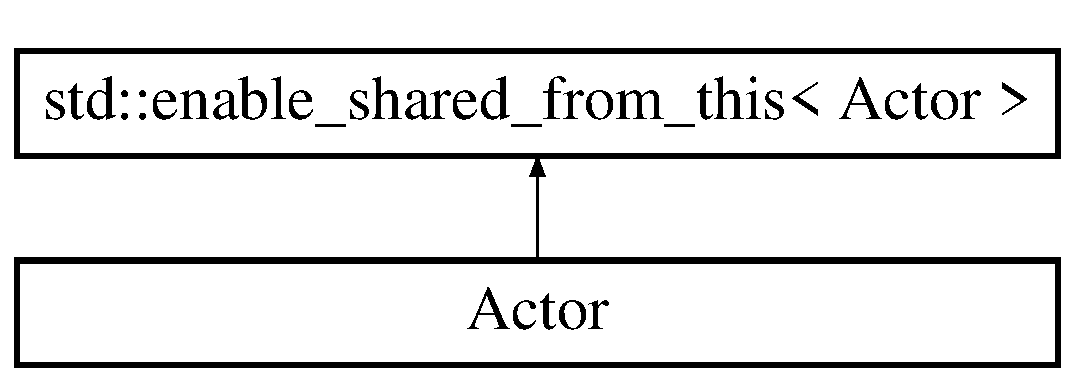
\includegraphics[height=2.000000cm]{class_actor}
\end{center}
\end{figure}
\subsection*{Public Member Functions}
\begin{DoxyCompactItemize}
\item 
\hyperlink{class_actor_a2a0ff4335a1ee9096df90f288c026c8b}{Actor} ()
\item 
\hyperlink{class_actor_ae4d47c1596ba6c1a872780864b7a57d6}{Actor} (string \hyperlink{class_actor_adc0a0fe742f4bd972168f8ef7ad55e8f}{name})
\item 
\hyperlink{class_actor_ad2f5e5c51e030e2297b1f934420e1cf8}{Actor} (\hyperlink{class_actor}{Actor} \&\&)=delete
\item 
virtual \hyperlink{class_actor_ad807fe8f85e72ab263a0c05e3231cb39}{$\sim$\+Actor} ()
\item 
\hypertarget{class_actor_a015e66865b31e58e6b6250a3fda088d6}{}shared\+\_\+ptr$<$ \hyperlink{class_actor}{Actor} $>$ {\bfseries clone} ()\label{class_actor_a015e66865b31e58e6b6250a3fda088d6}

\item 
void \hyperlink{class_actor_a56c0c99205523bf3c4dfd2e53180f375}{awake} ()
\item 
void \hyperlink{class_actor_a2ad907a434d65b64cc707813b4fdfa58}{tick} (float delta\+Seconds)
\item 
void \hyperlink{class_actor_afc18e8c46f392d2f8e73438a7bdef217}{trigger\+Physx\+Collision} (\hyperlink{class_actor}{Actor} $\ast$actor)
\item 
void \hyperlink{class_actor_adac69a3dfa2e0b449a28ecb064eab08f}{trigger\+Physx\+Trigger} (\hyperlink{class_actor}{Actor} $\ast$actor)
\item 
shared\+\_\+ptr$<$ \hyperlink{class_actor}{Actor} $>$ \hyperlink{class_actor_afa78edc729309614a051ac0114e8863e}{get\+Parent} ()
\item 
void \hyperlink{class_actor_a3efc64aa73b4b69dc3bc5b37154eadcc}{set\+Parent} (shared\+\_\+ptr$<$ \hyperlink{class_actor}{Actor} $>$ \hyperlink{class_actor_abb76f1796e97a76079f4d181f7fd1088}{parent})
\item 
void \hyperlink{class_actor_acb295666d6ec675b1a50ddb337954a4f}{add\+Children} (shared\+\_\+ptr$<$ \hyperlink{class_actor}{Actor} $>$ \hyperlink{class_actor_a572508685fe6f0387c5342d285c92b7f}{children})
\item 
void \hyperlink{class_actor_aec859bd1effede68867cfd6d5543249f}{set\+Active} (bool is\+Active)
\item 
bool \hyperlink{class_actor_a171bd8310af9bbaeed9ae45b74f3a1cf}{get\+Is\+Active} ()
\item 
void \hyperlink{class_actor_aeb08c0442fc1527d5e68e6f9d6cc9838}{set\+Editor\+Flag} (bool is\+Editor)
\item 
bool \hyperlink{class_actor_a89683da9b3aa1bd99ceec334c90e1a7b}{get\+Editor\+Flag} ()
\item 
void \hyperlink{class_actor_a12abcd53c7d35e55cb7eb43de049f1e5}{init\+Components} ()
\item 
void \hyperlink{class_actor_a7420eb679c14e07b90f3a777403cdad0}{add\+Component} (shared\+\_\+ptr$<$ \hyperlink{class_component}{Component} $>$ component)
\item 
\hypertarget{class_actor_a40a74338fb5a54d6ad2ee834d98d0643}{}void {\bfseries destroy\+Components} ()\label{class_actor_a40a74338fb5a54d6ad2ee834d98d0643}

\item 
{\footnotesize template$<$typename T $>$ }\\shared\+\_\+ptr$<$ T $>$ \hyperlink{class_actor_a3756af4dbe3b2ed513fe47afb081239d}{Add\+Component} ()
\item 
{\footnotesize template$<$typename T $>$ }\\shared\+\_\+ptr$<$ T $>$ \hyperlink{class_actor_ab8d69cb3d4fc68daf7120d9c207923f6}{Get\+Component} ()
\end{DoxyCompactItemize}
\subsection*{Public Attributes}
\begin{DoxyCompactItemize}
\item 
string \hyperlink{class_actor_adc0a0fe742f4bd972168f8ef7ad55e8f}{name}
\item 
shared\+\_\+ptr$<$ \hyperlink{class_transform}{Transform} $>$ \hyperlink{class_actor_a9b100f35016ff90eb2ff60ae39566a26}{transform}
\item 
vector$<$ shared\+\_\+ptr$<$ \hyperlink{class_component}{Component} $>$ $>$ \hyperlink{class_actor_afb92b26e5696d81dd5b512c2e41c00ea}{components}
\item 
weak\+\_\+ptr$<$ \hyperlink{class_actor}{Actor} $>$ \hyperlink{class_actor_abb76f1796e97a76079f4d181f7fd1088}{parent}
\item 
vector$<$ weak\+\_\+ptr$<$ \hyperlink{class_actor}{Actor} $>$ $>$ \hyperlink{class_actor_a572508685fe6f0387c5342d285c92b7f}{children}
\end{DoxyCompactItemize}


\subsection{Detailed Description}
\hyperlink{class_actor}{Actor}

\hyperlink{class_actor}{Actor} is the base \hyperlink{class_game}{Game} Object. Since G\+U\+Inity is a component-\/based engine, the idea is N\+O\+T to inherit from \hyperlink{class_actor}{Actor} to create new behaviours. On the contrary, every game object in the world should be an \hyperlink{class_actor}{Actor} and their behaviour should come from different components. 

\subsection{Constructor \& Destructor Documentation}
\hypertarget{class_actor_a2a0ff4335a1ee9096df90f288c026c8b}{}\index{Actor@{Actor}!Actor@{Actor}}
\index{Actor@{Actor}!Actor@{Actor}}
\subsubsection[{Actor()}]{\setlength{\rightskip}{0pt plus 5cm}Actor\+::\+Actor (
\begin{DoxyParamCaption}
{}
\end{DoxyParamCaption}
)\hspace{0.3cm}{\ttfamily [inline]}}\label{class_actor_a2a0ff4335a1ee9096df90f288c026c8b}
Default Constructor \hypertarget{class_actor_ae4d47c1596ba6c1a872780864b7a57d6}{}\index{Actor@{Actor}!Actor@{Actor}}
\index{Actor@{Actor}!Actor@{Actor}}
\subsubsection[{Actor(string name)}]{\setlength{\rightskip}{0pt plus 5cm}Actor\+::\+Actor (
\begin{DoxyParamCaption}
\item[{string}]{name}
\end{DoxyParamCaption}
)}\label{class_actor_ae4d47c1596ba6c1a872780864b7a57d6}
Constructor with actor name \hypertarget{class_actor_ad2f5e5c51e030e2297b1f934420e1cf8}{}\index{Actor@{Actor}!Actor@{Actor}}
\index{Actor@{Actor}!Actor@{Actor}}
\subsubsection[{Actor(\+Actor \&\&)=delete}]{\setlength{\rightskip}{0pt plus 5cm}Actor\+::\+Actor (
\begin{DoxyParamCaption}
\item[{{\bf Actor} \&\&}]{}
\end{DoxyParamCaption}
)\hspace{0.3cm}{\ttfamily [delete]}}\label{class_actor_ad2f5e5c51e030e2297b1f934420e1cf8}
Prevent move constructor \hypertarget{class_actor_ad807fe8f85e72ab263a0c05e3231cb39}{}\index{Actor@{Actor}!````~Actor@{$\sim$\+Actor}}
\index{````~Actor@{$\sim$\+Actor}!Actor@{Actor}}
\subsubsection[{$\sim$\+Actor()}]{\setlength{\rightskip}{0pt plus 5cm}Actor\+::$\sim$\+Actor (
\begin{DoxyParamCaption}
{}
\end{DoxyParamCaption}
)\hspace{0.3cm}{\ttfamily [virtual]}}\label{class_actor_ad807fe8f85e72ab263a0c05e3231cb39}
Default Destructor 

\subsection{Member Function Documentation}
\hypertarget{class_actor_acb295666d6ec675b1a50ddb337954a4f}{}\index{Actor@{Actor}!add\+Children@{add\+Children}}
\index{add\+Children@{add\+Children}!Actor@{Actor}}
\subsubsection[{add\+Children(shared\+\_\+ptr$<$ Actor $>$ children)}]{\setlength{\rightskip}{0pt plus 5cm}void Actor\+::add\+Children (
\begin{DoxyParamCaption}
\item[{shared\+\_\+ptr$<$ {\bf Actor} $>$}]{children}
\end{DoxyParamCaption}
)}\label{class_actor_acb295666d6ec675b1a50ddb337954a4f}
Add children to list \hypertarget{class_actor_a7420eb679c14e07b90f3a777403cdad0}{}\index{Actor@{Actor}!add\+Component@{add\+Component}}
\index{add\+Component@{add\+Component}!Actor@{Actor}}
\subsubsection[{add\+Component(shared\+\_\+ptr$<$ Component $>$ component)}]{\setlength{\rightskip}{0pt plus 5cm}void Actor\+::add\+Component (
\begin{DoxyParamCaption}
\item[{shared\+\_\+ptr$<$ {\bf Component} $>$}]{component}
\end{DoxyParamCaption}
)}\label{class_actor_a7420eb679c14e07b90f3a777403cdad0}
add\+Component. Attaches an existing component to the actor. This function is used for deserialization of Actors \hypertarget{class_actor_a3756af4dbe3b2ed513fe47afb081239d}{}\index{Actor@{Actor}!Add\+Component@{Add\+Component}}
\index{Add\+Component@{Add\+Component}!Actor@{Actor}}
\subsubsection[{Add\+Component()}]{\setlength{\rightskip}{0pt plus 5cm}template$<$typename T $>$ shared\+\_\+ptr$<$T$>$ Actor\+::\+Add\+Component (
\begin{DoxyParamCaption}
{}
\end{DoxyParamCaption}
)\hspace{0.3cm}{\ttfamily [inline]}}\label{class_actor_a3756af4dbe3b2ed513fe47afb081239d}
Generic Add\+Component. This function creates a smart pointer to the desired component and returns it \hypertarget{class_actor_a56c0c99205523bf3c4dfd2e53180f375}{}\index{Actor@{Actor}!awake@{awake}}
\index{awake@{awake}!Actor@{Actor}}
\subsubsection[{awake()}]{\setlength{\rightskip}{0pt plus 5cm}void Actor\+::awake (
\begin{DoxyParamCaption}
{}
\end{DoxyParamCaption}
)}\label{class_actor_a56c0c99205523bf3c4dfd2e53180f375}
Awake. This function is called to Awake all the components attached to the actor \hypertarget{class_actor_ab8d69cb3d4fc68daf7120d9c207923f6}{}\index{Actor@{Actor}!Get\+Component@{Get\+Component}}
\index{Get\+Component@{Get\+Component}!Actor@{Actor}}
\subsubsection[{Get\+Component()}]{\setlength{\rightskip}{0pt plus 5cm}template$<$typename T $>$ shared\+\_\+ptr$<$T$>$ Actor\+::\+Get\+Component (
\begin{DoxyParamCaption}
{}
\end{DoxyParamCaption}
)\hspace{0.3cm}{\ttfamily [inline]}}\label{class_actor_ab8d69cb3d4fc68daf7120d9c207923f6}
Generic Get\+Component. This function looks for a component of the desired type from the components list and returns the first it finds \hypertarget{class_actor_a89683da9b3aa1bd99ceec334c90e1a7b}{}\index{Actor@{Actor}!get\+Editor\+Flag@{get\+Editor\+Flag}}
\index{get\+Editor\+Flag@{get\+Editor\+Flag}!Actor@{Actor}}
\subsubsection[{get\+Editor\+Flag()}]{\setlength{\rightskip}{0pt plus 5cm}bool Actor\+::get\+Editor\+Flag (
\begin{DoxyParamCaption}
{}
\end{DoxyParamCaption}
)}\label{class_actor_a89683da9b3aa1bd99ceec334c90e1a7b}
editor\+Flat getter

editor\+Flag setter \hypertarget{class_actor_a171bd8310af9bbaeed9ae45b74f3a1cf}{}\index{Actor@{Actor}!get\+Is\+Active@{get\+Is\+Active}}
\index{get\+Is\+Active@{get\+Is\+Active}!Actor@{Actor}}
\subsubsection[{get\+Is\+Active()}]{\setlength{\rightskip}{0pt plus 5cm}bool Actor\+::get\+Is\+Active (
\begin{DoxyParamCaption}
{}
\end{DoxyParamCaption}
)}\label{class_actor_a171bd8310af9bbaeed9ae45b74f3a1cf}
is\+Active getter \hypertarget{class_actor_afa78edc729309614a051ac0114e8863e}{}\index{Actor@{Actor}!get\+Parent@{get\+Parent}}
\index{get\+Parent@{get\+Parent}!Actor@{Actor}}
\subsubsection[{get\+Parent()}]{\setlength{\rightskip}{0pt plus 5cm}shared\+\_\+ptr$<$ {\bf Actor} $>$ Actor\+::get\+Parent (
\begin{DoxyParamCaption}
{}
\end{DoxyParamCaption}
)}\label{class_actor_afa78edc729309614a051ac0114e8863e}
Parent getter \hypertarget{class_actor_a12abcd53c7d35e55cb7eb43de049f1e5}{}\index{Actor@{Actor}!init\+Components@{init\+Components}}
\index{init\+Components@{init\+Components}!Actor@{Actor}}
\subsubsection[{init\+Components()}]{\setlength{\rightskip}{0pt plus 5cm}void Actor\+::init\+Components (
\begin{DoxyParamCaption}
{}
\end{DoxyParamCaption}
)}\label{class_actor_a12abcd53c7d35e55cb7eb43de049f1e5}
init\+Components. This function is called to Initialize all the components attached to the actor \hypertarget{class_actor_aec859bd1effede68867cfd6d5543249f}{}\index{Actor@{Actor}!set\+Active@{set\+Active}}
\index{set\+Active@{set\+Active}!Actor@{Actor}}
\subsubsection[{set\+Active(bool is\+Active)}]{\setlength{\rightskip}{0pt plus 5cm}void Actor\+::set\+Active (
\begin{DoxyParamCaption}
\item[{bool}]{is\+Active}
\end{DoxyParamCaption}
)}\label{class_actor_aec859bd1effede68867cfd6d5543249f}
is\+Active setter \hypertarget{class_actor_aeb08c0442fc1527d5e68e6f9d6cc9838}{}\index{Actor@{Actor}!set\+Editor\+Flag@{set\+Editor\+Flag}}
\index{set\+Editor\+Flag@{set\+Editor\+Flag}!Actor@{Actor}}
\subsubsection[{set\+Editor\+Flag(bool is\+Editor)}]{\setlength{\rightskip}{0pt plus 5cm}void Actor\+::set\+Editor\+Flag (
\begin{DoxyParamCaption}
\item[{bool}]{is\+Editor}
\end{DoxyParamCaption}
)}\label{class_actor_aeb08c0442fc1527d5e68e6f9d6cc9838}
editor\+Flat setter

editor\+Flag setter \hypertarget{class_actor_a3efc64aa73b4b69dc3bc5b37154eadcc}{}\index{Actor@{Actor}!set\+Parent@{set\+Parent}}
\index{set\+Parent@{set\+Parent}!Actor@{Actor}}
\subsubsection[{set\+Parent(shared\+\_\+ptr$<$ Actor $>$ parent)}]{\setlength{\rightskip}{0pt plus 5cm}void Actor\+::set\+Parent (
\begin{DoxyParamCaption}
\item[{shared\+\_\+ptr$<$ {\bf Actor} $>$}]{parent}
\end{DoxyParamCaption}
)}\label{class_actor_a3efc64aa73b4b69dc3bc5b37154eadcc}
Parent setter \hypertarget{class_actor_a2ad907a434d65b64cc707813b4fdfa58}{}\index{Actor@{Actor}!tick@{tick}}
\index{tick@{tick}!Actor@{Actor}}
\subsubsection[{tick(float delta\+Seconds)}]{\setlength{\rightskip}{0pt plus 5cm}void Actor\+::tick (
\begin{DoxyParamCaption}
\item[{float}]{delta\+Seconds}
\end{DoxyParamCaption}
)}\label{class_actor_a2ad907a434d65b64cc707813b4fdfa58}
Tick. Function called every frame. This function is responsible for calling the Tick for each \hyperlink{class_component}{Component} attached to the actor \hypertarget{class_actor_afc18e8c46f392d2f8e73438a7bdef217}{}\index{Actor@{Actor}!trigger\+Physx\+Collision@{trigger\+Physx\+Collision}}
\index{trigger\+Physx\+Collision@{trigger\+Physx\+Collision}!Actor@{Actor}}
\subsubsection[{trigger\+Physx\+Collision(\+Actor $\ast$actor)}]{\setlength{\rightskip}{0pt plus 5cm}void Actor\+::trigger\+Physx\+Collision (
\begin{DoxyParamCaption}
\item[{{\bf Actor} $\ast$}]{actor}
\end{DoxyParamCaption}
)}\label{class_actor_afc18e8c46f392d2f8e73438a7bdef217}
Function that receives Collision from Phys\+X  -\/ Other actor that collided with this

Function that receives Collision from Phys\+X  -\/ Other actor that collided with this

Delegates the collision to all Script\+Components. Trying to emulate Unity, where every script can contain code to handle Collision \hypertarget{class_actor_adac69a3dfa2e0b449a28ecb064eab08f}{}\index{Actor@{Actor}!trigger\+Physx\+Trigger@{trigger\+Physx\+Trigger}}
\index{trigger\+Physx\+Trigger@{trigger\+Physx\+Trigger}!Actor@{Actor}}
\subsubsection[{trigger\+Physx\+Trigger(\+Actor $\ast$actor)}]{\setlength{\rightskip}{0pt plus 5cm}void Actor\+::trigger\+Physx\+Trigger (
\begin{DoxyParamCaption}
\item[{{\bf Actor} $\ast$}]{actor}
\end{DoxyParamCaption}
)}\label{class_actor_adac69a3dfa2e0b449a28ecb064eab08f}
Function that receives Trigger Collision from Phys\+X  -\/ Other actor that collided with this

Function that receives Trigger Collision from Phys\+X  -\/ Other actor that collided with this

Delegates the collision to all Script\+Components. Trying to emulate Unity, where every script can contain code to handle Collision 

\subsection{Member Data Documentation}
\hypertarget{class_actor_a572508685fe6f0387c5342d285c92b7f}{}\index{Actor@{Actor}!children@{children}}
\index{children@{children}!Actor@{Actor}}
\subsubsection[{children}]{\setlength{\rightskip}{0pt plus 5cm}vector$<$weak\+\_\+ptr$<${\bf Actor}$>$ $>$ Actor\+::children}\label{class_actor_a572508685fe6f0387c5342d285c92b7f}
Children. All the Actors that are children of this. Weak\+\_\+ptr because we don\textquotesingle{}t want this object to prevent an \hyperlink{class_actor}{Actor} to be destroyed \hypertarget{class_actor_afb92b26e5696d81dd5b512c2e41c00ea}{}\index{Actor@{Actor}!components@{components}}
\index{components@{components}!Actor@{Actor}}
\subsubsection[{components}]{\setlength{\rightskip}{0pt plus 5cm}vector$<$shared\+\_\+ptr$<${\bf Component}$>$ $>$ Actor\+::components}\label{class_actor_afb92b26e5696d81dd5b512c2e41c00ea}
The components of the \hyperlink{class_actor}{Actor}, may vary from \hyperlink{class_collider}{Collider} to Script \hypertarget{class_actor_adc0a0fe742f4bd972168f8ef7ad55e8f}{}\index{Actor@{Actor}!name@{name}}
\index{name@{name}!Actor@{Actor}}
\subsubsection[{name}]{\setlength{\rightskip}{0pt plus 5cm}string Actor\+::name}\label{class_actor_adc0a0fe742f4bd972168f8ef7ad55e8f}
Name of the \hyperlink{class_actor}{Actor} \hypertarget{class_actor_abb76f1796e97a76079f4d181f7fd1088}{}\index{Actor@{Actor}!parent@{parent}}
\index{parent@{parent}!Actor@{Actor}}
\subsubsection[{parent}]{\setlength{\rightskip}{0pt plus 5cm}weak\+\_\+ptr$<${\bf Actor}$>$ Actor\+::parent}\label{class_actor_abb76f1796e97a76079f4d181f7fd1088}
Parent. Actors can have parent to create hierarchy. Hierarchy is important to group several Actors into one Weak\+\_\+ptr because we don\textquotesingle{}t want this object to prevent an \hyperlink{class_actor}{Actor} to be destroyed \hypertarget{class_actor_a9b100f35016ff90eb2ff60ae39566a26}{}\index{Actor@{Actor}!transform@{transform}}
\index{transform@{transform}!Actor@{Actor}}
\subsubsection[{transform}]{\setlength{\rightskip}{0pt plus 5cm}shared\+\_\+ptr$<${\bf Transform}$>$ Actor\+::transform}\label{class_actor_a9b100f35016ff90eb2ff60ae39566a26}
\hyperlink{class_transform}{Transform} of the \hyperlink{class_actor}{Actor}. By default every \hyperlink{class_actor}{Actor} has a transform. For further improvements, it could be considered to treat \hyperlink{class_transform}{Transform} as any other component 

The documentation for this class was generated from the following files\+:\begin{DoxyCompactItemize}
\item 
/\+Users/guilherme\+\_\+cunha/\+Dev/\+G\+I\+T\+H\+U\+B/\+G\+U\+Inity/\+Source/Actor.\+hpp\item 
/\+Users/guilherme\+\_\+cunha/\+Dev/\+G\+I\+T\+H\+U\+B/\+G\+U\+Inity/\+Source/Actor.\+cpp\end{DoxyCompactItemize}

\hypertarget{struct_actor_description}{}\section{Actor\+Description Struct Reference}
\label{struct_actor_description}\index{Actor\+Description@{Actor\+Description}}
\subsection*{Public Attributes}
\begin{DoxyCompactItemize}
\item 
\hypertarget{struct_actor_description_ae5a739a425bed5c2bb5ec29453e50951}{}string {\bfseries name}\label{struct_actor_description_ae5a739a425bed5c2bb5ec29453e50951}

\item 
\hypertarget{struct_actor_description_afa78d4071f58976818b990e11d34b5ba}{}bool {\bfseries is\+Active}\label{struct_actor_description_afa78d4071f58976818b990e11d34b5ba}

\item 
\hypertarget{struct_actor_description_a05fceac8009484292a14b70ed1cfd12a}{}bool {\bfseries editor\+Flag}\label{struct_actor_description_a05fceac8009484292a14b70ed1cfd12a}

\item 
\hypertarget{struct_actor_description_a8aed8b63b24be0d28b73b7d00feac4f5}{}\hyperlink{struct_transform_description}{Transform\+Description} {\bfseries transform}\label{struct_actor_description_a8aed8b63b24be0d28b73b7d00feac4f5}

\end{DoxyCompactItemize}


The documentation for this struct was generated from the following file\+:\begin{DoxyCompactItemize}
\item 
/\+Users/guilherme\+\_\+cunha/\+Dev/\+G\+I\+T\+H\+U\+B/\+G\+U\+Inity/\+Source/Serialization\+Structs.\+hpp\end{DoxyCompactItemize}

\hypertarget{class_add_force_script}{}\section{Add\+Force\+Script Class Reference}
\label{class_add_force_script}\index{Add\+Force\+Script@{Add\+Force\+Script}}
Inheritance diagram for Add\+Force\+Script\+:\begin{figure}[H]
\begin{center}
\leavevmode
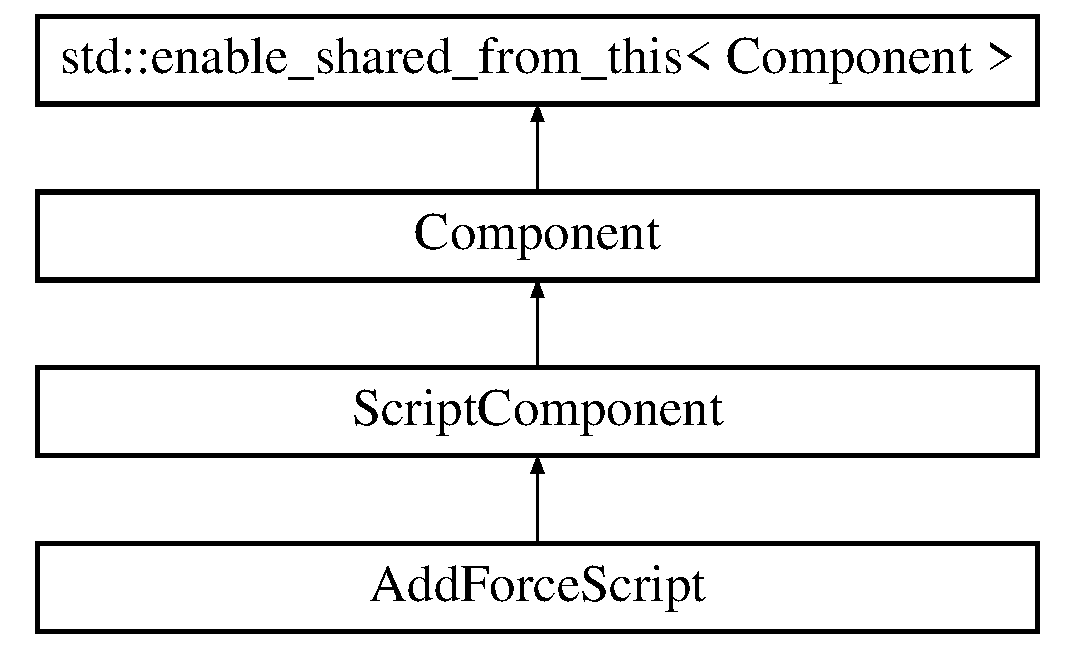
\includegraphics[height=4.000000cm]{class_add_force_script}
\end{center}
\end{figure}
\subsection*{Public Member Functions}
\begin{DoxyCompactItemize}
\item 
void \hyperlink{class_add_force_script_a8ad91eeecbfae666a28c44345d59251d}{tick} (float delta\+Seconds) override
\end{DoxyCompactItemize}
\subsection*{Additional Inherited Members}


\subsection{Member Function Documentation}
\hypertarget{class_add_force_script_a8ad91eeecbfae666a28c44345d59251d}{}\index{Add\+Force\+Script@{Add\+Force\+Script}!tick@{tick}}
\index{tick@{tick}!Add\+Force\+Script@{Add\+Force\+Script}}
\subsubsection[{tick(float delta\+Seconds) override}]{\setlength{\rightskip}{0pt plus 5cm}void Add\+Force\+Script\+::tick (
\begin{DoxyParamCaption}
\item[{float}]{delta\+Secods}
\end{DoxyParamCaption}
)\hspace{0.3cm}{\ttfamily [override]}, {\ttfamily [virtual]}}\label{class_add_force_script_a8ad91eeecbfae666a28c44345d59251d}
\hyperlink{class_component}{Component} tick override 
\begin{DoxyParams}[1]{Parameters}
\mbox{\tt in}  & {\em delta\+Seconds} & last frame durations \\
\hline
\end{DoxyParams}


Reimplemented from \hyperlink{class_script_component_aa765fa62a343a8d83eb168d369b93a51}{Script\+Component}.



The documentation for this class was generated from the following files\+:\begin{DoxyCompactItemize}
\item 
/\+Users/guilherme\+\_\+cunha/\+Dev/\+G\+I\+T\+H\+U\+B/\+G\+U\+Inity/\+Source/Add\+Force\+Script.\+hpp\item 
/\+Users/guilherme\+\_\+cunha/\+Dev/\+G\+I\+T\+H\+U\+B/\+G\+U\+Inity/\+Source/Add\+Force\+Script.\+cpp\end{DoxyCompactItemize}

\hypertarget{classany__type}{}\section{any\+\_\+type Class Reference}
\label{classany__type}\index{any\+\_\+type@{any\+\_\+type}}
Inheritance diagram for any\+\_\+type\+:\begin{figure}[H]
\begin{center}
\leavevmode
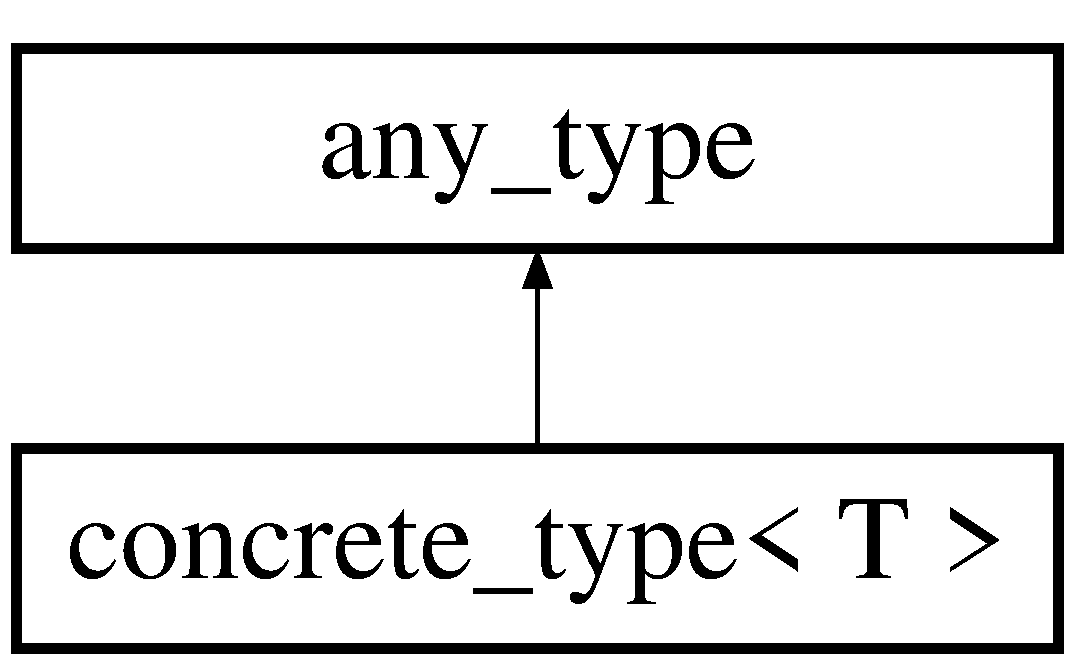
\includegraphics[height=2.000000cm]{classany__type}
\end{center}
\end{figure}
\subsection*{Public Member Functions}
\begin{DoxyCompactItemize}
\item 
\hypertarget{classany__type_aa0c205b7997b79173ba337fd90be4922}{}virtual void {\bfseries print} ()=0\label{classany__type_aa0c205b7997b79173ba337fd90be4922}

\end{DoxyCompactItemize}


The documentation for this class was generated from the following file\+:\begin{DoxyCompactItemize}
\item 
/\+Users/guilherme\+\_\+cunha/\+Dev/\+G\+I\+T\+H\+U\+B/\+G\+U\+Inity/\+Source/Any\+Class.\+hpp\end{DoxyCompactItemize}

\hypertarget{class_asset}{}\section{Asset Class Reference}
\label{class_asset}\index{Asset@{Asset}}


{\ttfamily \#include $<$Asset.\+hpp$>$}

Inheritance diagram for Asset\+:\begin{figure}[H]
\begin{center}
\leavevmode
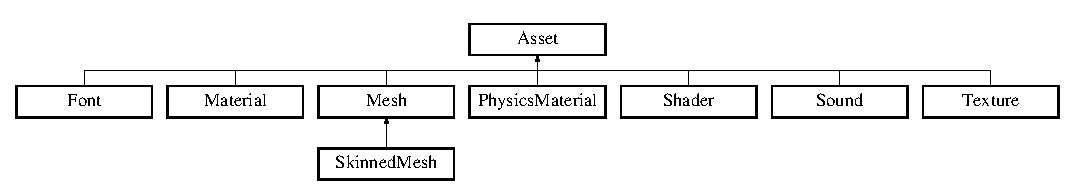
\includegraphics[height=2.181818cm]{class_asset}
\end{center}
\end{figure}
\subsection*{Public Member Functions}
\begin{DoxyCompactItemize}
\item 
\hyperlink{class_asset_aae5517f0d77f2fbadaebef7a6988ec25}{Asset} ()
\item 
virtual \hyperlink{class_asset_a2cdb921599e4fdf8fc2e0ce5dd9266ee}{$\sim$\+Asset} ()
\item 
void \hyperlink{class_asset_a920b3238cad8063ca1482dfaedd95a5c}{set\+Asset\+I\+D} (unsigned int new\+Asset\+I\+D)
\item 
unsigned int \hyperlink{class_asset_ac5bf03127f4aa3f192efa7e0bbc80d6c}{get\+Asset\+I\+D} () const 
\item 
string \hyperlink{class_asset_afab04bc636b88dc6fb8735a959611cec}{get\+Path} ()
\item 
void \hyperlink{class_asset_a9d565be1462466aa491a2dfaeeed9c5b}{set\+Path} (string new\+Path)
\item 
void \hyperlink{class_asset_aa9591848b238fa4a43e2f7f8118a8fae}{set\+Name} (string name)
\item 
string \hyperlink{class_asset_aa550074b9d3da8e65ff3164f0cadfd4f}{get\+Name} ()
\item 
void \hyperlink{class_asset_a77fe2f2a76ea9c3c8ee11567079956e0}{set\+C\+R\+C} (int crc)
\item 
int \hyperlink{class_asset_a3accd92508b7b3df783c5eb67b88adfb}{set\+C\+R\+C} ()
\end{DoxyCompactItemize}


\subsection{Detailed Description}
Class \hyperlink{class_asset}{Asset}. This class represents assets in game. This can vary from textures to meshes and audio files. Virtually, everything that can be serialized to a file is an \hyperlink{class_asset}{Asset}. Currently, these are the assets\+: -\/\+Texture -\/\+Font -\/\+Audio -\/\+Mesh

The idea is to simulate the Assets folder in Unity. Therefore, assets place in a folder should be loaded automatically. Each \hyperlink{class_asset}{Asset} has a C\+R\+C (checksum) to check if the file has changed or not. 

\subsection{Constructor \& Destructor Documentation}
\hypertarget{class_asset_aae5517f0d77f2fbadaebef7a6988ec25}{}\index{Asset@{Asset}!Asset@{Asset}}
\index{Asset@{Asset}!Asset@{Asset}}
\subsubsection[{Asset()}]{\setlength{\rightskip}{0pt plus 5cm}Asset\+::\+Asset (
\begin{DoxyParamCaption}
{}
\end{DoxyParamCaption}
)\hspace{0.3cm}{\ttfamily [inline]}}\label{class_asset_aae5517f0d77f2fbadaebef7a6988ec25}
Default Constructor \hypertarget{class_asset_a2cdb921599e4fdf8fc2e0ce5dd9266ee}{}\index{Asset@{Asset}!````~Asset@{$\sim$\+Asset}}
\index{````~Asset@{$\sim$\+Asset}!Asset@{Asset}}
\subsubsection[{$\sim$\+Asset()}]{\setlength{\rightskip}{0pt plus 5cm}virtual Asset\+::$\sim$\+Asset (
\begin{DoxyParamCaption}
{}
\end{DoxyParamCaption}
)\hspace{0.3cm}{\ttfamily [inline]}, {\ttfamily [virtual]}}\label{class_asset_a2cdb921599e4fdf8fc2e0ce5dd9266ee}
Default Destructor -\/ Virtual because it\textquotesingle{}s a parent class 

\subsection{Member Function Documentation}
\hypertarget{class_asset_ac5bf03127f4aa3f192efa7e0bbc80d6c}{}\index{Asset@{Asset}!get\+Asset\+I\+D@{get\+Asset\+I\+D}}
\index{get\+Asset\+I\+D@{get\+Asset\+I\+D}!Asset@{Asset}}
\subsubsection[{get\+Asset\+I\+D() const }]{\setlength{\rightskip}{0pt plus 5cm}unsigned int Asset\+::get\+Asset\+I\+D (
\begin{DoxyParamCaption}
{}
\end{DoxyParamCaption}
) const\hspace{0.3cm}{\ttfamily [inline]}}\label{class_asset_ac5bf03127f4aa3f192efa7e0bbc80d6c}
asset\+I\+D getter \hypertarget{class_asset_aa550074b9d3da8e65ff3164f0cadfd4f}{}\index{Asset@{Asset}!get\+Name@{get\+Name}}
\index{get\+Name@{get\+Name}!Asset@{Asset}}
\subsubsection[{get\+Name()}]{\setlength{\rightskip}{0pt plus 5cm}string Asset\+::get\+Name (
\begin{DoxyParamCaption}
{}
\end{DoxyParamCaption}
)\hspace{0.3cm}{\ttfamily [inline]}}\label{class_asset_aa550074b9d3da8e65ff3164f0cadfd4f}
name getter \hypertarget{class_asset_afab04bc636b88dc6fb8735a959611cec}{}\index{Asset@{Asset}!get\+Path@{get\+Path}}
\index{get\+Path@{get\+Path}!Asset@{Asset}}
\subsubsection[{get\+Path()}]{\setlength{\rightskip}{0pt plus 5cm}string Asset\+::get\+Path (
\begin{DoxyParamCaption}
{}
\end{DoxyParamCaption}
)\hspace{0.3cm}{\ttfamily [inline]}}\label{class_asset_afab04bc636b88dc6fb8735a959611cec}
Full path getter \hypertarget{class_asset_a920b3238cad8063ca1482dfaedd95a5c}{}\index{Asset@{Asset}!set\+Asset\+I\+D@{set\+Asset\+I\+D}}
\index{set\+Asset\+I\+D@{set\+Asset\+I\+D}!Asset@{Asset}}
\subsubsection[{set\+Asset\+I\+D(unsigned int new\+Asset\+I\+D)}]{\setlength{\rightskip}{0pt plus 5cm}void Asset\+::set\+Asset\+I\+D (
\begin{DoxyParamCaption}
\item[{unsigned int}]{new\+Asset\+I\+D}
\end{DoxyParamCaption}
)\hspace{0.3cm}{\ttfamily [inline]}}\label{class_asset_a920b3238cad8063ca1482dfaedd95a5c}
asset\+I\+D setter \hypertarget{class_asset_a77fe2f2a76ea9c3c8ee11567079956e0}{}\index{Asset@{Asset}!set\+C\+R\+C@{set\+C\+R\+C}}
\index{set\+C\+R\+C@{set\+C\+R\+C}!Asset@{Asset}}
\subsubsection[{set\+C\+R\+C(int crc)}]{\setlength{\rightskip}{0pt plus 5cm}void Asset\+::set\+C\+R\+C (
\begin{DoxyParamCaption}
\item[{int}]{crc}
\end{DoxyParamCaption}
)\hspace{0.3cm}{\ttfamily [inline]}}\label{class_asset_a77fe2f2a76ea9c3c8ee11567079956e0}
C\+R\+C setter \hypertarget{class_asset_a3accd92508b7b3df783c5eb67b88adfb}{}\index{Asset@{Asset}!set\+C\+R\+C@{set\+C\+R\+C}}
\index{set\+C\+R\+C@{set\+C\+R\+C}!Asset@{Asset}}
\subsubsection[{set\+C\+R\+C()}]{\setlength{\rightskip}{0pt plus 5cm}int Asset\+::set\+C\+R\+C (
\begin{DoxyParamCaption}
{}
\end{DoxyParamCaption}
)\hspace{0.3cm}{\ttfamily [inline]}}\label{class_asset_a3accd92508b7b3df783c5eb67b88adfb}
C\+R\+C getter \hypertarget{class_asset_aa9591848b238fa4a43e2f7f8118a8fae}{}\index{Asset@{Asset}!set\+Name@{set\+Name}}
\index{set\+Name@{set\+Name}!Asset@{Asset}}
\subsubsection[{set\+Name(string name)}]{\setlength{\rightskip}{0pt plus 5cm}void Asset\+::set\+Name (
\begin{DoxyParamCaption}
\item[{string}]{name}
\end{DoxyParamCaption}
)\hspace{0.3cm}{\ttfamily [inline]}}\label{class_asset_aa9591848b238fa4a43e2f7f8118a8fae}
name setter \hypertarget{class_asset_a9d565be1462466aa491a2dfaeeed9c5b}{}\index{Asset@{Asset}!set\+Path@{set\+Path}}
\index{set\+Path@{set\+Path}!Asset@{Asset}}
\subsubsection[{set\+Path(string new\+Path)}]{\setlength{\rightskip}{0pt plus 5cm}void Asset\+::set\+Path (
\begin{DoxyParamCaption}
\item[{string}]{new\+Path}
\end{DoxyParamCaption}
)\hspace{0.3cm}{\ttfamily [inline]}}\label{class_asset_a9d565be1462466aa491a2dfaeeed9c5b}
Full path setter 

The documentation for this class was generated from the following file\+:\begin{DoxyCompactItemize}
\item 
/\+Users/guilherme\+\_\+cunha/\+Dev/\+G\+I\+T\+H\+U\+B/\+G\+U\+Inity/\+Source/Asset.\+hpp\end{DoxyCompactItemize}

\hypertarget{class_asset_database}{}\section{Asset\+Database Class Reference}
\label{class_asset_database}\index{Asset\+Database@{Asset\+Database}}


{\ttfamily \#include $<$Asset\+Database.\+hpp$>$}

\subsection*{Static Public Member Functions}
\begin{DoxyCompactItemize}
\item 
static void \hyperlink{class_asset_database_ae7102ec2e1c01fff217946fe03b4b8a4}{init} ()
\item 
static void \hyperlink{class_asset_database_a61392880e1fff5ec7b1c4cd31812efd1}{shutdown} ()
\item 
static void \hyperlink{class_asset_database_af81f7154e7e779974b776e76a4650277}{read\+Serialiation\+File} (string full\+Path)
\item 
static void \hyperlink{class_asset_database_a0277280f887d471a7f9a14102d6ea4a5}{create\+Serialization\+File} (shared\+\_\+ptr$<$ \hyperlink{class_asset}{Asset} $>$ asset, string filename)
\item 
static void \hyperlink{class_asset_database_a6929177caebd34d42dec699f19838fe1}{load\+All\+Meta\+Files} ()
\item 
{\footnotesize template$<$class T $>$ }\\static shared\+\_\+ptr$<$ T $>$ \hyperlink{class_asset_database_a9168af02cf1d567a8eb92184b69a0994}{get\+Asset} (string name)
\item 
static shared\+\_\+ptr$<$ \hyperlink{class_asset}{Asset} $>$ \hyperlink{class_asset_database_a03fc428514f43aad4c098261a5ee64d9}{get\+Asset} (unsigned int asset\+I\+D)
\item 
{\footnotesize template$<$typename T $>$ }\\static void \hyperlink{class_asset_database_ad6746e08dba5a75e8ed9869cdddd5652}{assign\+Current\+I\+D} (T asset, string name)
\item 
{\footnotesize template$<$typename T $>$ }\\static void \hyperlink{class_asset_database_a4a5dafe295b51eb6f779d7bae90c86c8}{assign\+Current\+I\+D} (T asset)
\item 
static shared\+\_\+ptr$<$ \hyperlink{class_asset}{Asset} $>$ \hyperlink{class_asset_database_a327f2cbdf751c34ee9cfa3f17631d6bc}{try\+Load\+Asset} (string file, string extension)
\item 
static shared\+\_\+ptr$<$ \hyperlink{class_shader}{Shader} $>$ \hyperlink{class_asset_database_a472ae1d457b43252efd740299f515fa5}{create\+Shader} (string name, string vs\+Filename, string fs\+Filename)
\item 
static shared\+\_\+ptr$<$ \hyperlink{class_material}{Material} $>$ \hyperlink{class_asset_database_a21fb8c80540611ed1a8fb32b273c8177}{create\+Material} (string name, shared\+\_\+ptr$<$ \hyperlink{class_shader}{Shader} $>$ shader)
\item 
static shared\+\_\+ptr$<$ \hyperlink{class_physics_material}{Physics\+Material} $>$ \hyperlink{class_asset_database_ad724e4ceb50db68af5a6d13b1359b112}{create\+Physics\+Material} (string name, float friction, float dynamic\+Friction, float restitution)
\item 
static shared\+\_\+ptr$<$ \hyperlink{class_mesh}{Mesh} $>$ \hyperlink{class_asset_database_ab5793b0cd769426e4fb31626cc863850}{create\+Mesh\+From\+F\+B\+X} (string filename)
\item 
static shared\+\_\+ptr$<$ \hyperlink{class_mesh}{Mesh} $>$ \hyperlink{class_asset_database_adb9836fa33d82c3b58a2133cc072e2d2}{create\+Mesh\+From\+O\+B\+J} (string filename)
\item 
static shared\+\_\+ptr$<$ \hyperlink{class_mesh}{Mesh} $>$ \hyperlink{class_asset_database_a5228eaa4dbb587dd1d4c7ae4e69402da}{create\+Mesh} (vector$<$ \hyperlink{struct_mesh_vertex}{Mesh\+Vertex} $>$ vertex, vector$<$ unsigned short $>$ triangles)
\item 
static shared\+\_\+ptr$<$ \hyperlink{class_sound}{Sound} $>$ \hyperlink{class_asset_database_aab4df6c6999d752fce7a222c1f79f224}{create\+Sound} (string filename)
\item 
static shared\+\_\+ptr$<$ \hyperlink{class_texture}{Texture} $>$ \hyperlink{class_asset_database_a85240fb09c76bf851d4bb10bd0cfc77a}{create\+Texture} (string filename)
\item 
static shared\+\_\+ptr$<$ \hyperlink{class_font}{Font} $>$ \hyperlink{class_asset_database_ae558252480890d40daefc38b7e8d3d7a}{create\+Font} (string filename, int font\+Size)
\end{DoxyCompactItemize}


\subsection{Detailed Description}
\hyperlink{class_asset_database}{Asset\+Database} is a static class that creates and holds all user Assets (exceptions are the assets used by the system). The idea is to simulate Unity\textquotesingle{}s \hyperlink{class_asset}{Asset} folder, making sure that whenever a file is added, it\textquotesingle{}s automatically loaded. 

\subsection{Member Function Documentation}
\hypertarget{class_asset_database_ad6746e08dba5a75e8ed9869cdddd5652}{}\index{Asset\+Database@{Asset\+Database}!assign\+Current\+I\+D@{assign\+Current\+I\+D}}
\index{assign\+Current\+I\+D@{assign\+Current\+I\+D}!Asset\+Database@{Asset\+Database}}
\subsubsection[{assign\+Current\+I\+D(\+T asset, string name)}]{\setlength{\rightskip}{0pt plus 5cm}template$<$typename T $>$ void Asset\+Database\+::assign\+Current\+I\+D (
\begin{DoxyParamCaption}
\item[{T}]{asset, }
\item[{string}]{name}
\end{DoxyParamCaption}
)\hspace{0.3cm}{\ttfamily [static]}}\label{class_asset_database_ad6746e08dba5a75e8ed9869cdddd5652}
assign\+Current\+I\+D. Increments the primary key and add the \hyperlink{class_asset}{Asset} to the maps with the proper name. \hypertarget{class_asset_database_a4a5dafe295b51eb6f779d7bae90c86c8}{}\index{Asset\+Database@{Asset\+Database}!assign\+Current\+I\+D@{assign\+Current\+I\+D}}
\index{assign\+Current\+I\+D@{assign\+Current\+I\+D}!Asset\+Database@{Asset\+Database}}
\subsubsection[{assign\+Current\+I\+D(\+T asset)}]{\setlength{\rightskip}{0pt plus 5cm}template$<$typename T $>$ void Asset\+Database\+::assign\+Current\+I\+D (
\begin{DoxyParamCaption}
\item[{T}]{asset}
\end{DoxyParamCaption}
)\hspace{0.3cm}{\ttfamily [static]}}\label{class_asset_database_a4a5dafe295b51eb6f779d7bae90c86c8}
assign\+Current\+I\+D. Increments the primary key and add the \hyperlink{class_asset}{Asset} to the maps. Uses the asset\+I\+D as the name \hypertarget{class_asset_database_ae558252480890d40daefc38b7e8d3d7a}{}\index{Asset\+Database@{Asset\+Database}!create\+Font@{create\+Font}}
\index{create\+Font@{create\+Font}!Asset\+Database@{Asset\+Database}}
\subsubsection[{create\+Font(string filename, int font\+Size)}]{\setlength{\rightskip}{0pt plus 5cm}shared\+\_\+ptr$<$ {\bf Font} $>$ Asset\+Database\+::create\+Font (
\begin{DoxyParamCaption}
\item[{string}]{filename, }
\item[{int}]{font\+Size}
\end{DoxyParamCaption}
)\hspace{0.3cm}{\ttfamily [static]}}\label{class_asset_database_ae558252480890d40daefc38b7e8d3d7a}
Create \hyperlink{class_font}{Font} from .ttf file. \hypertarget{class_asset_database_a21fb8c80540611ed1a8fb32b273c8177}{}\index{Asset\+Database@{Asset\+Database}!create\+Material@{create\+Material}}
\index{create\+Material@{create\+Material}!Asset\+Database@{Asset\+Database}}
\subsubsection[{create\+Material(string name, shared\+\_\+ptr$<$ Shader $>$ shader)}]{\setlength{\rightskip}{0pt plus 5cm}shared\+\_\+ptr$<$ {\bf Material} $>$ Asset\+Database\+::create\+Material (
\begin{DoxyParamCaption}
\item[{string}]{filename, }
\item[{shared\+\_\+ptr$<$ {\bf Shader} $>$}]{shader}
\end{DoxyParamCaption}
)\hspace{0.3cm}{\ttfamily [static]}}\label{class_asset_database_a21fb8c80540611ed1a8fb32b273c8177}
Create material from a shader. Several materials can have the same shader but different properties, such as textures and colors. \hypertarget{class_asset_database_a5228eaa4dbb587dd1d4c7ae4e69402da}{}\index{Asset\+Database@{Asset\+Database}!create\+Mesh@{create\+Mesh}}
\index{create\+Mesh@{create\+Mesh}!Asset\+Database@{Asset\+Database}}
\subsubsection[{create\+Mesh(vector$<$ Mesh\+Vertex $>$ vertex, vector$<$ unsigned short $>$ triangles)}]{\setlength{\rightskip}{0pt plus 5cm}shared\+\_\+ptr$<$ {\bf Mesh} $>$ Asset\+Database\+::create\+Mesh (
\begin{DoxyParamCaption}
\item[{vector$<$ {\bf Mesh\+Vertex} $>$}]{vertex, }
\item[{vector$<$ unsigned short $>$}]{triangles}
\end{DoxyParamCaption}
)\hspace{0.3cm}{\ttfamily [static]}}\label{class_asset_database_a5228eaa4dbb587dd1d4c7ae4e69402da}
Create mesh from list of vertice data and triangles \hypertarget{class_asset_database_ab5793b0cd769426e4fb31626cc863850}{}\index{Asset\+Database@{Asset\+Database}!create\+Mesh\+From\+F\+B\+X@{create\+Mesh\+From\+F\+B\+X}}
\index{create\+Mesh\+From\+F\+B\+X@{create\+Mesh\+From\+F\+B\+X}!Asset\+Database@{Asset\+Database}}
\subsubsection[{create\+Mesh\+From\+F\+B\+X(string filename)}]{\setlength{\rightskip}{0pt plus 5cm}shared\+\_\+ptr$<$ {\bf Mesh} $>$ Asset\+Database\+::create\+Mesh\+From\+F\+B\+X (
\begin{DoxyParamCaption}
\item[{string}]{filename}
\end{DoxyParamCaption}
)\hspace{0.3cm}{\ttfamily [static]}}\label{class_asset_database_ab5793b0cd769426e4fb31626cc863850}
Create mesh from .fbx files \hypertarget{class_asset_database_adb9836fa33d82c3b58a2133cc072e2d2}{}\index{Asset\+Database@{Asset\+Database}!create\+Mesh\+From\+O\+B\+J@{create\+Mesh\+From\+O\+B\+J}}
\index{create\+Mesh\+From\+O\+B\+J@{create\+Mesh\+From\+O\+B\+J}!Asset\+Database@{Asset\+Database}}
\subsubsection[{create\+Mesh\+From\+O\+B\+J(string filename)}]{\setlength{\rightskip}{0pt plus 5cm}shared\+\_\+ptr$<$ {\bf Mesh} $>$ Asset\+Database\+::create\+Mesh\+From\+O\+B\+J (
\begin{DoxyParamCaption}
\item[{string}]{filename}
\end{DoxyParamCaption}
)\hspace{0.3cm}{\ttfamily [static]}}\label{class_asset_database_adb9836fa33d82c3b58a2133cc072e2d2}
Create mesh from .obj files \hypertarget{class_asset_database_ad724e4ceb50db68af5a6d13b1359b112}{}\index{Asset\+Database@{Asset\+Database}!create\+Physics\+Material@{create\+Physics\+Material}}
\index{create\+Physics\+Material@{create\+Physics\+Material}!Asset\+Database@{Asset\+Database}}
\subsubsection[{create\+Physics\+Material(string name, float friction, float dynamic\+Friction, float restitution)}]{\setlength{\rightskip}{0pt plus 5cm}shared\+\_\+ptr$<$ {\bf Physics\+Material} $>$ Asset\+Database\+::create\+Physics\+Material (
\begin{DoxyParamCaption}
\item[{string}]{name, }
\item[{float}]{friction, }
\item[{float}]{dynamic\+Friction, }
\item[{float}]{restitution}
\end{DoxyParamCaption}
)\hspace{0.3cm}{\ttfamily [static]}}\label{class_asset_database_ad724e4ceb50db68af5a6d13b1359b112}
Create a physics material that can be used to specify behaviour of shapes in the physics scene \hypertarget{class_asset_database_a0277280f887d471a7f9a14102d6ea4a5}{}\index{Asset\+Database@{Asset\+Database}!create\+Serialization\+File@{create\+Serialization\+File}}
\index{create\+Serialization\+File@{create\+Serialization\+File}!Asset\+Database@{Asset\+Database}}
\subsubsection[{create\+Serialization\+File(shared\+\_\+ptr$<$ Asset $>$ asset, string filename)}]{\setlength{\rightskip}{0pt plus 5cm}void Asset\+Database\+::create\+Serialization\+File (
\begin{DoxyParamCaption}
\item[{shared\+\_\+ptr$<$ {\bf Asset} $>$}]{asset, }
\item[{string}]{filename}
\end{DoxyParamCaption}
)\hspace{0.3cm}{\ttfamily [static]}}\label{class_asset_database_a0277280f887d471a7f9a14102d6ea4a5}
create\+Serialization\+File. Create a meta-\/file for an asset (Serialize an asset) \hypertarget{class_asset_database_a472ae1d457b43252efd740299f515fa5}{}\index{Asset\+Database@{Asset\+Database}!create\+Shader@{create\+Shader}}
\index{create\+Shader@{create\+Shader}!Asset\+Database@{Asset\+Database}}
\subsubsection[{create\+Shader(string name, string vs\+Filename, string fs\+Filename)}]{\setlength{\rightskip}{0pt plus 5cm}shared\+\_\+ptr$<$ {\bf Shader} $>$ Asset\+Database\+::create\+Shader (
\begin{DoxyParamCaption}
\item[{string}]{filename, }
\item[{string}]{vs\+Filename, }
\item[{string}]{fs\+Filename}
\end{DoxyParamCaption}
)\hspace{0.3cm}{\ttfamily [static]}}\label{class_asset_database_a472ae1d457b43252efd740299f515fa5}
Create shader from a vertex shader and a fragment shader. Name is the name of the newly created shader \hypertarget{class_asset_database_aab4df6c6999d752fce7a222c1f79f224}{}\index{Asset\+Database@{Asset\+Database}!create\+Sound@{create\+Sound}}
\index{create\+Sound@{create\+Sound}!Asset\+Database@{Asset\+Database}}
\subsubsection[{create\+Sound(string filename)}]{\setlength{\rightskip}{0pt plus 5cm}shared\+\_\+ptr$<$ {\bf Sound} $>$ Asset\+Database\+::create\+Sound (
\begin{DoxyParamCaption}
\item[{string}]{filename}
\end{DoxyParamCaption}
)\hspace{0.3cm}{\ttfamily [static]}}\label{class_asset_database_aab4df6c6999d752fce7a222c1f79f224}
Create empty mesh. Used for Font\+Meshes that dynamicaly create the mesh Create \hyperlink{class_sound}{Sound} asset from file.

Create \hyperlink{class_sound}{Sound} asset from file. \hypertarget{class_asset_database_a85240fb09c76bf851d4bb10bd0cfc77a}{}\index{Asset\+Database@{Asset\+Database}!create\+Texture@{create\+Texture}}
\index{create\+Texture@{create\+Texture}!Asset\+Database@{Asset\+Database}}
\subsubsection[{create\+Texture(string filename)}]{\setlength{\rightskip}{0pt plus 5cm}shared\+\_\+ptr$<$ {\bf Texture} $>$ Asset\+Database\+::create\+Texture (
\begin{DoxyParamCaption}
\item[{string}]{filename}
\end{DoxyParamCaption}
)\hspace{0.3cm}{\ttfamily [static]}}\label{class_asset_database_a85240fb09c76bf851d4bb10bd0cfc77a}
Create \hyperlink{class_texture}{Texture} from file. Only supported file is .png in the moment. \hypertarget{class_asset_database_a9168af02cf1d567a8eb92184b69a0994}{}\index{Asset\+Database@{Asset\+Database}!get\+Asset@{get\+Asset}}
\index{get\+Asset@{get\+Asset}!Asset\+Database@{Asset\+Database}}
\subsubsection[{get\+Asset(string name)}]{\setlength{\rightskip}{0pt plus 5cm}template$<$class T $>$ static shared\+\_\+ptr$<$T$>$ Asset\+Database\+::get\+Asset (
\begin{DoxyParamCaption}
\item[{string}]{name}
\end{DoxyParamCaption}
)\hspace{0.3cm}{\ttfamily [inline]}, {\ttfamily [static]}}\label{class_asset_database_a9168af02cf1d567a8eb92184b69a0994}
Search on the database for the asset with name==filename. \hypertarget{class_asset_database_a03fc428514f43aad4c098261a5ee64d9}{}\index{Asset\+Database@{Asset\+Database}!get\+Asset@{get\+Asset}}
\index{get\+Asset@{get\+Asset}!Asset\+Database@{Asset\+Database}}
\subsubsection[{get\+Asset(unsigned int asset\+I\+D)}]{\setlength{\rightskip}{0pt plus 5cm}shared\+\_\+ptr$<$ {\bf Asset} $>$ Asset\+Database\+::get\+Asset (
\begin{DoxyParamCaption}
\item[{unsigned int}]{asset\+I\+D}
\end{DoxyParamCaption}
)\hspace{0.3cm}{\ttfamily [static]}}\label{class_asset_database_a03fc428514f43aad4c098261a5ee64d9}
Search on the database for the asset with asset\+I\+D==asset\+I\+D.

Search on the database for the asset with asset\+I\+D==Asset.\+asset\+I\+D. \hypertarget{class_asset_database_ae7102ec2e1c01fff217946fe03b4b8a4}{}\index{Asset\+Database@{Asset\+Database}!init@{init}}
\index{init@{init}!Asset\+Database@{Asset\+Database}}
\subsubsection[{init()}]{\setlength{\rightskip}{0pt plus 5cm}void Asset\+Database\+::init (
\begin{DoxyParamCaption}
{}
\end{DoxyParamCaption}
)\hspace{0.3cm}{\ttfamily [static]}}\label{class_asset_database_ae7102ec2e1c01fff217946fe03b4b8a4}
init. Function that initializes the class. Initialize the \hyperlink{class_mesh}{Mesh} Importer \hypertarget{class_asset_database_a6929177caebd34d42dec699f19838fe1}{}\index{Asset\+Database@{Asset\+Database}!load\+All\+Meta\+Files@{load\+All\+Meta\+Files}}
\index{load\+All\+Meta\+Files@{load\+All\+Meta\+Files}!Asset\+Database@{Asset\+Database}}
\subsubsection[{load\+All\+Meta\+Files()}]{\setlength{\rightskip}{0pt plus 5cm}void Asset\+Database\+::load\+All\+Meta\+Files (
\begin{DoxyParamCaption}
{}
\end{DoxyParamCaption}
)\hspace{0.3cm}{\ttfamily [static]}}\label{class_asset_database_a6929177caebd34d42dec699f19838fe1}
Once serialization is done and working, the \hyperlink{class_asset_database}{Asset\+Database} should not reload all files everytime. It should load only the \hyperlink{class_asset}{Asset} Description (.meta$<$-\/$>$.desc) file and check if it\textquotesingle{}s up to date

Once serialization is done and working, the \hyperlink{class_asset_database}{Asset\+Database} should not reload all files everytime. It should load only the \hyperlink{class_asset}{Asset} Description (.meta//.desc) file and check if it\textquotesingle{}s up to date. This function loads all the meta-\/files existing in the Common\+Data folder \hypertarget{class_asset_database_af81f7154e7e779974b776e76a4650277}{}\index{Asset\+Database@{Asset\+Database}!read\+Serialiation\+File@{read\+Serialiation\+File}}
\index{read\+Serialiation\+File@{read\+Serialiation\+File}!Asset\+Database@{Asset\+Database}}
\subsubsection[{read\+Serialiation\+File(string full\+Path)}]{\setlength{\rightskip}{0pt plus 5cm}void Asset\+Database\+::read\+Serialiation\+File (
\begin{DoxyParamCaption}
\item[{string}]{full\+Path}
\end{DoxyParamCaption}
)\hspace{0.3cm}{\ttfamily [static]}}\label{class_asset_database_af81f7154e7e779974b776e76a4650277}
read\+Serialiation\+File. Loads an asset from a description file (Deserialize an asset)

read\+Serialiation\+File. Loads an asset from a description file. \hypertarget{class_asset_database_a61392880e1fff5ec7b1c4cd31812efd1}{}\index{Asset\+Database@{Asset\+Database}!shutdown@{shutdown}}
\index{shutdown@{shutdown}!Asset\+Database@{Asset\+Database}}
\subsubsection[{shutdown()}]{\setlength{\rightskip}{0pt plus 5cm}void Asset\+Database\+::shutdown (
\begin{DoxyParamCaption}
{}
\end{DoxyParamCaption}
)\hspace{0.3cm}{\ttfamily [static]}}\label{class_asset_database_a61392880e1fff5ec7b1c4cd31812efd1}
shutdown. Releases allocated memmory Shutdown the \hyperlink{class_mesh}{Mesh} Importer \hypertarget{class_asset_database_a327f2cbdf751c34ee9cfa3f17631d6bc}{}\index{Asset\+Database@{Asset\+Database}!try\+Load\+Asset@{try\+Load\+Asset}}
\index{try\+Load\+Asset@{try\+Load\+Asset}!Asset\+Database@{Asset\+Database}}
\subsubsection[{try\+Load\+Asset(string file, string extension)}]{\setlength{\rightskip}{0pt plus 5cm}shared\+\_\+ptr$<$ {\bf Asset} $>$ Asset\+Database\+::try\+Load\+Asset (
\begin{DoxyParamCaption}
\item[{string}]{file, }
\item[{string}]{extension}
\end{DoxyParamCaption}
)\hspace{0.3cm}{\ttfamily [static]}}\label{class_asset_database_a327f2cbdf751c34ee9cfa3f17631d6bc}
try\+Load\+Asset. Delegates the file to the appropriate loader. 

The documentation for this class was generated from the following files\+:\begin{DoxyCompactItemize}
\item 
/\+Users/guilherme\+\_\+cunha/\+Dev/\+G\+I\+T\+H\+U\+B/\+G\+U\+Inity/\+Source/Asset\+Database.\+hpp\item 
/\+Users/guilherme\+\_\+cunha/\+Dev/\+G\+I\+T\+H\+U\+B/\+G\+U\+Inity/\+Source/Asset\+Database.\+cpp\end{DoxyCompactItemize}

\hypertarget{class_box_collider}{}\section{Box\+Collider Class Reference}
\label{class_box_collider}\index{Box\+Collider@{Box\+Collider}}


{\ttfamily \#include $<$Box\+Collider.\+hpp$>$}

Inheritance diagram for Box\+Collider\+:\begin{figure}[H]
\begin{center}
\leavevmode
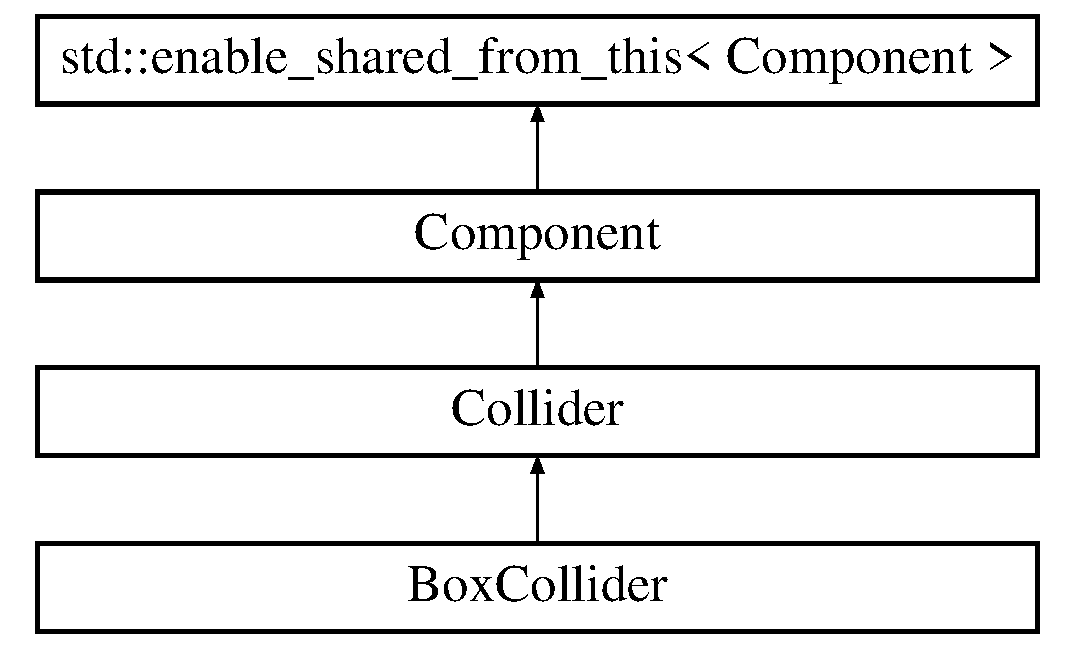
\includegraphics[height=4.000000cm]{class_box_collider}
\end{center}
\end{figure}
\subsection*{Public Member Functions}
\begin{DoxyCompactItemize}
\item 
\hyperlink{class_box_collider_aa8358aaf4f5fae5446ebdf0b303ccce3}{Box\+Collider} ()
\item 
\hyperlink{class_box_collider_a13f840ee628a62add163a77aea76224b}{Box\+Collider} (Px\+Vec3 half\+Extent, Px\+Vec3 \hyperlink{class_collider_a42b57aa35ab665daf89ae844e479c560}{center}=Px\+Vec3(0, 0, 0))
\item 
virtual \hyperlink{class_box_collider_a8c33dbb4325d76d441de38b7c4ae43af}{$\sim$\+Box\+Collider} ()
\item 
virtual void \hyperlink{class_box_collider_ad98ff62ff6b5c48dc8f18b1a2d2429e4}{init} ()
\item 
virtual shared\+\_\+ptr$<$ \hyperlink{class_component}{Component} $>$ \hyperlink{class_box_collider_ab9154438078b0fb9d33f2f8958e3a71e}{clone} () override
\item 
virtual shared\+\_\+ptr$<$ \hyperlink{class_component_description}{Component\+Description} $>$ \hyperlink{group__serialization__functions_gad0cea24e9390a50ce68178944128cfab}{get\+Component\+Description} () override
\item 
virtual void \hyperlink{group__serialization__functions_ga495b07647b7b0c2a843be54180dab9e4}{deserialize} (shared\+\_\+ptr$<$ \hyperlink{class_component_description}{Component\+Description} $>$ desc) override
\end{DoxyCompactItemize}
\subsection*{Additional Inherited Members}


\subsection{Detailed Description}
\hyperlink{class_box_collider}{Box\+Collider} is an A\+A\+B\+B collider \hyperlink{class_component}{Component}. Can either be real physics simulated or trigger only. 

\subsection{Constructor \& Destructor Documentation}
\hypertarget{class_box_collider_aa8358aaf4f5fae5446ebdf0b303ccce3}{}\index{Box\+Collider@{Box\+Collider}!Box\+Collider@{Box\+Collider}}
\index{Box\+Collider@{Box\+Collider}!Box\+Collider@{Box\+Collider}}
\subsubsection[{Box\+Collider()}]{\setlength{\rightskip}{0pt plus 5cm}Box\+Collider\+::\+Box\+Collider (
\begin{DoxyParamCaption}
{}
\end{DoxyParamCaption}
)}\label{class_box_collider_aa8358aaf4f5fae5446ebdf0b303ccce3}
Default Constructor \hypertarget{class_box_collider_a13f840ee628a62add163a77aea76224b}{}\index{Box\+Collider@{Box\+Collider}!Box\+Collider@{Box\+Collider}}
\index{Box\+Collider@{Box\+Collider}!Box\+Collider@{Box\+Collider}}
\subsubsection[{Box\+Collider(\+Px\+Vec3 half\+Extent, Px\+Vec3 center=\+Px\+Vec3(0, 0, 0))}]{\setlength{\rightskip}{0pt plus 5cm}Box\+Collider\+::\+Box\+Collider (
\begin{DoxyParamCaption}
\item[{Px\+Vec3}]{half\+Extent, }
\item[{Px\+Vec3}]{center = {\ttfamily PxVec3(0,0,0)}}
\end{DoxyParamCaption}
)}\label{class_box_collider_a13f840ee628a62add163a77aea76224b}
Deserialization Constructor \hypertarget{class_box_collider_a8c33dbb4325d76d441de38b7c4ae43af}{}\index{Box\+Collider@{Box\+Collider}!````~Box\+Collider@{$\sim$\+Box\+Collider}}
\index{````~Box\+Collider@{$\sim$\+Box\+Collider}!Box\+Collider@{Box\+Collider}}
\subsubsection[{$\sim$\+Box\+Collider()}]{\setlength{\rightskip}{0pt plus 5cm}Box\+Collider\+::$\sim$\+Box\+Collider (
\begin{DoxyParamCaption}
{}
\end{DoxyParamCaption}
)\hspace{0.3cm}{\ttfamily [virtual]}}\label{class_box_collider_a8c33dbb4325d76d441de38b7c4ae43af}
Default Destructor 

\subsection{Member Function Documentation}
\hypertarget{class_box_collider_ab9154438078b0fb9d33f2f8958e3a71e}{}\index{Box\+Collider@{Box\+Collider}!clone@{clone}}
\index{clone@{clone}!Box\+Collider@{Box\+Collider}}
\subsubsection[{clone() override}]{\setlength{\rightskip}{0pt plus 5cm}shared\+\_\+ptr$<$ {\bf Component} $>$ Box\+Collider\+::clone (
\begin{DoxyParamCaption}
{}
\end{DoxyParamCaption}
)\hspace{0.3cm}{\ttfamily [override]}, {\ttfamily [virtual]}}\label{class_box_collider_ab9154438078b0fb9d33f2f8958e3a71e}
Clones current component (Prototype Design Pattern) \begin{DoxyReturn}{Returns}
shared\+\_\+ptr to cloned \hyperlink{class_box_collider}{Box\+Collider} \hyperlink{class_component}{Component} 
\end{DoxyReturn}


Implements \hyperlink{class_collider_a28d0829db9804b27590afc9979e61a1c}{Collider}.

\hypertarget{class_box_collider_ad98ff62ff6b5c48dc8f18b1a2d2429e4}{}\index{Box\+Collider@{Box\+Collider}!init@{init}}
\index{init@{init}!Box\+Collider@{Box\+Collider}}
\subsubsection[{init()}]{\setlength{\rightskip}{0pt plus 5cm}void Box\+Collider\+::init (
\begin{DoxyParamCaption}
{}
\end{DoxyParamCaption}
)\hspace{0.3cm}{\ttfamily [virtual]}}\label{class_box_collider_ad98ff62ff6b5c48dc8f18b1a2d2429e4}
Init component override. Create a new Box Shape in the Phys\+X scene. 

Reimplemented from \hyperlink{class_collider_aed04ad82be15bcba1d3dc6a09f76dae6}{Collider}.



The documentation for this class was generated from the following files\+:\begin{DoxyCompactItemize}
\item 
/\+Users/guilherme\+\_\+cunha/\+Dev/\+G\+I\+T\+H\+U\+B/\+G\+U\+Inity/\+Source/Box\+Collider.\+hpp\item 
/\+Users/guilherme\+\_\+cunha/\+Dev/\+G\+I\+T\+H\+U\+B/\+G\+U\+Inity/\+Source/Box\+Collider.\+cpp\end{DoxyCompactItemize}

\hypertarget{class_box_collider_description}{}\section{Box\+Collider\+Description Class Reference}
\label{class_box_collider_description}\index{Box\+Collider\+Description@{Box\+Collider\+Description}}
Inheritance diagram for Box\+Collider\+Description\+:\begin{figure}[H]
\begin{center}
\leavevmode
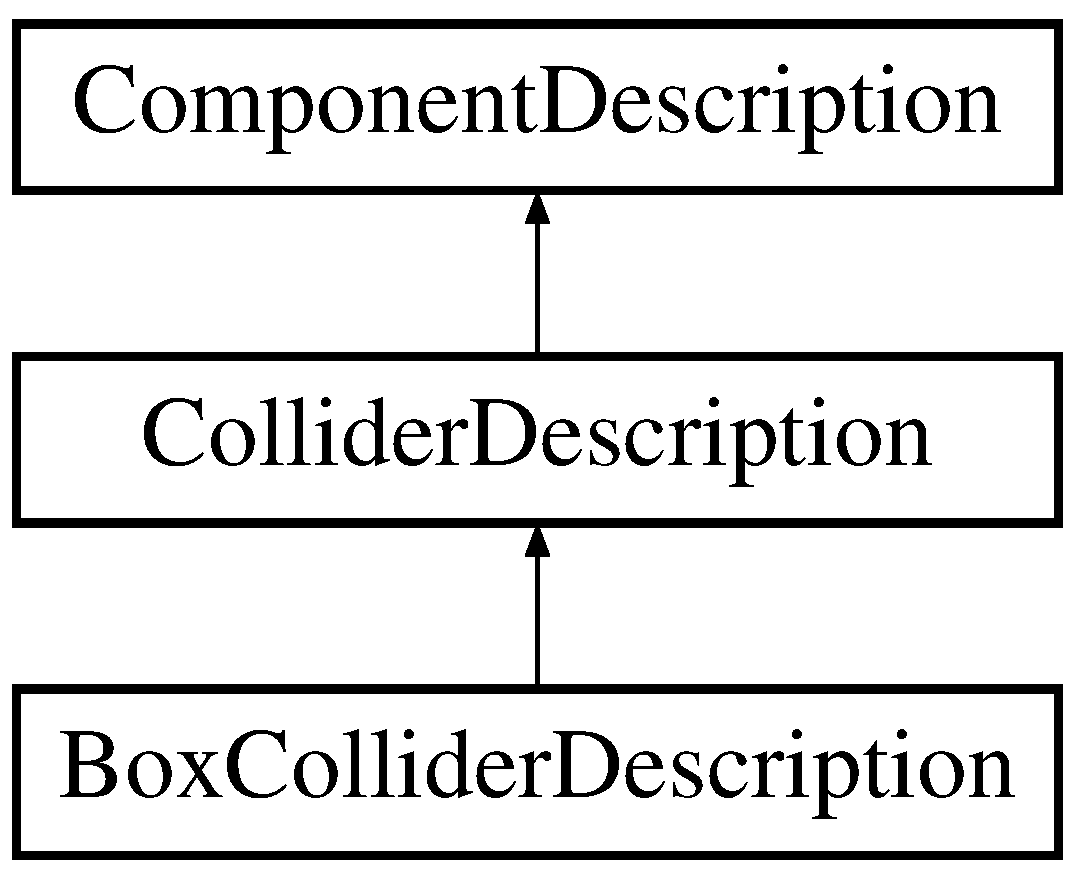
\includegraphics[height=3.000000cm]{class_box_collider_description}
\end{center}
\end{figure}
\subsection*{Public Member Functions}
\begin{DoxyCompactItemize}
\item 
\hypertarget{class_box_collider_description_aeb4b0b95f200e50eedb2b48fcdb09b80}{}{\bfseries Box\+Collider\+Description} (Px\+Vec3 half\+Ext)\label{class_box_collider_description_aeb4b0b95f200e50eedb2b48fcdb09b80}

\end{DoxyCompactItemize}
\subsection*{Public Attributes}
\begin{DoxyCompactItemize}
\item 
\hypertarget{class_box_collider_description_ac15affc1552dc9505b787ef6d6a05571}{}Px\+Vec3 {\bfseries half\+Extent}\label{class_box_collider_description_ac15affc1552dc9505b787ef6d6a05571}

\end{DoxyCompactItemize}


The documentation for this class was generated from the following file\+:\begin{DoxyCompactItemize}
\item 
/\+Users/guilherme\+\_\+cunha/\+Dev/\+G\+I\+T\+H\+U\+B/\+G\+U\+Inity/\+Source/Serialization\+Structs.\+hpp\end{DoxyCompactItemize}

\hypertarget{class_camera}{}\section{Camera Class Reference}
\label{class_camera}\index{Camera@{Camera}}


{\ttfamily \#include $<$Camera.\+hpp$>$}

Inheritance diagram for Camera\+:\begin{figure}[H]
\begin{center}
\leavevmode
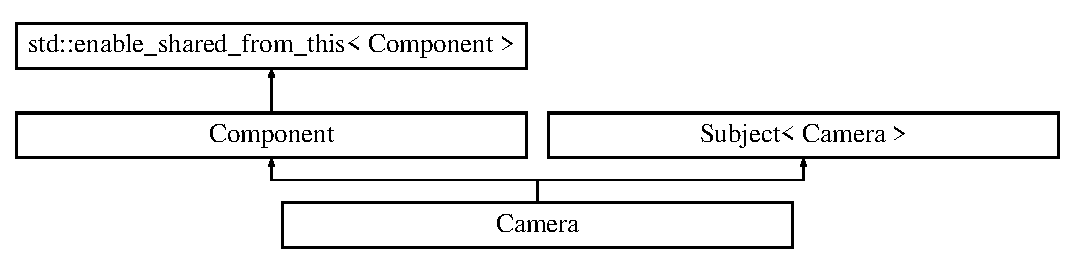
\includegraphics[height=3.000000cm]{class_camera}
\end{center}
\end{figure}
\subsection*{Public Member Functions}
\begin{DoxyCompactItemize}
\item 
\hyperlink{class_camera_a01f94c3543f56ede7af49dc778f19331}{Camera} ()
\item 
\hyperlink{class_camera_a80beb3602cfdb96013c7acb71de1510b}{Camera} (float near\+Clip\+Plane, float far\+Clip\+Plane, float fov, float ratio)
\item 
virtual \hyperlink{class_camera_ad1897942d0ccf91052386388a497349f}{$\sim$\+Camera} ()
\item 
void \hyperlink{class_camera_aba99909b33d24822c337c09aaabea242}{compute\+Model\+View\+Matrix} ()
\item 
glm\+::mat4 \hyperlink{class_camera_a295d9433395f9dc8ef664614b8024e13}{get\+Model\+Matrix} ()
\item 
glm\+::mat4 \hyperlink{class_camera_a218f84bd3fedb1635241844c95112fa4}{get\+M\+V\+P\+Matrix} ()
\item 
glm\+::mat4 \hyperlink{class_camera_adf09522521723786b9f405c99d6594c7}{get\+Projection\+Matrix} ()
\item 
glm\+::mat4 \hyperlink{class_camera_a5569ca5967e01d3344fbf6aba36d9820}{get\+View\+Matrix} ()
\item 
float \hyperlink{class_camera_a5db47defc06bb2e0b2f5e6297ccb6344}{get\+Near\+Clip} ()
\item 
float \hyperlink{class_camera_a1a5b0c8c2bc2af5c8c6ae47a53010add}{get\+Far\+Clip} ()
\item 
float \hyperlink{class_camera_a5ec1871e6f296d8528e64157c6371c09}{get\+F\+O\+V} ()
\item 
float \hyperlink{class_camera_aef9d5b443588a64ae649ef0d063f72f7}{get\+Screen\+Ratio} ()
\item 
glm\+::vec3 \hyperlink{class_camera_aca6735f228da3a95703a93b732f0eae3}{screen\+Point\+To\+World} (glm\+::vec2 pos)
\item 
\hyperlink{class_ray}{Ray} \hyperlink{class_camera_aed1084771ca34b01476779f024bd6af0}{screen\+Point\+To\+Ray} (glm\+::vec2 pos)
\item 
\hyperlink{class_ray}{Ray} \hyperlink{class_camera_a1cdd077539fbff108015287660570662}{screen\+Point\+To\+Ray2} (glm\+::vec2 pos)
\item 
virtual void \hyperlink{class_camera_aa575c1bbde6ae31425e233f0204af38c}{init} () override
\item 
virtual void \hyperlink{class_camera_a994622d61d20af75b2e86f5e39b01299}{destroy} () override
\item 
virtual void \hyperlink{class_camera_adec93b934ee03e786a949fbc2b9d169e}{awake} () override
\item 
virtual void \hyperlink{class_camera_a8a9acaa6d1b9b5265fa714d0e24e9aee}{tick} (float delta\+Secods) override
\item 
virtual shared\+\_\+ptr$<$ \hyperlink{class_component}{Component} $>$ \hyperlink{class_camera_a0d6043b74adb8fc9d8f8aaa66ea19aa3}{clone} () override
\item 
virtual shared\+\_\+ptr$<$ \hyperlink{class_component_description}{Component\+Description} $>$ \hyperlink{group__serialization__functions_gaf6a6ed08cfe3a456a1c38650c30a7231}{get\+Component\+Description} () override
\item 
virtual void \hyperlink{group__serialization__functions_gad2a03326aa3e8101471160c36058bd6c}{deserialize} (shared\+\_\+ptr$<$ \hyperlink{class_component_description}{Component\+Description} $>$ desc) override
\end{DoxyCompactItemize}
\subsection*{Additional Inherited Members}


\subsection{Detailed Description}
\hyperlink{class_camera}{Camera} \hyperlink{class_component}{Component}. This component simulates a camera in a 3\+D environment. It\textquotesingle{}s the point of view used for rendering the Actors of the \hyperlink{class_world}{World} 

\subsection{Constructor \& Destructor Documentation}
\hypertarget{class_camera_a01f94c3543f56ede7af49dc778f19331}{}\index{Camera@{Camera}!Camera@{Camera}}
\index{Camera@{Camera}!Camera@{Camera}}
\subsubsection[{Camera()}]{\setlength{\rightskip}{0pt plus 5cm}Camera\+::\+Camera (
\begin{DoxyParamCaption}
{}
\end{DoxyParamCaption}
)}\label{class_camera_a01f94c3543f56ede7af49dc778f19331}
Default Constructor \hypertarget{class_camera_a80beb3602cfdb96013c7acb71de1510b}{}\index{Camera@{Camera}!Camera@{Camera}}
\index{Camera@{Camera}!Camera@{Camera}}
\subsubsection[{Camera(float near\+Clip\+Plane, float far\+Clip\+Plane, float fov, float ratio)}]{\setlength{\rightskip}{0pt plus 5cm}Camera\+::\+Camera (
\begin{DoxyParamCaption}
\item[{float}]{near\+Clip\+Plane, }
\item[{float}]{far\+Clip\+Plane, }
\item[{float}]{fov, }
\item[{float}]{ratio}
\end{DoxyParamCaption}
)}\label{class_camera_a80beb3602cfdb96013c7acb71de1510b}
Constructor with custom parameters near clip plane, far clip plane, field of vision and screen ratio. \hypertarget{class_camera_ad1897942d0ccf91052386388a497349f}{}\index{Camera@{Camera}!````~Camera@{$\sim$\+Camera}}
\index{````~Camera@{$\sim$\+Camera}!Camera@{Camera}}
\subsubsection[{$\sim$\+Camera()}]{\setlength{\rightskip}{0pt plus 5cm}Camera\+::$\sim$\+Camera (
\begin{DoxyParamCaption}
{}
\end{DoxyParamCaption}
)\hspace{0.3cm}{\ttfamily [virtual]}}\label{class_camera_ad1897942d0ccf91052386388a497349f}
Default Destructor. Virtual because inherits \hyperlink{class_component}{Component} 

\subsection{Member Function Documentation}
\hypertarget{class_camera_adec93b934ee03e786a949fbc2b9d169e}{}\index{Camera@{Camera}!awake@{awake}}
\index{awake@{awake}!Camera@{Camera}}
\subsubsection[{awake() override}]{\setlength{\rightskip}{0pt plus 5cm}void Camera\+::awake (
\begin{DoxyParamCaption}
{}
\end{DoxyParamCaption}
)\hspace{0.3cm}{\ttfamily [override]}, {\ttfamily [virtual]}}\label{class_camera_adec93b934ee03e786a949fbc2b9d169e}
\hyperlink{class_component}{Component} awake override. Computes M\+V\+P\+Matrix 

Reimplemented from \hyperlink{class_component_ae413974ecdbc8f65c6ff707b84278b0e}{Component}.

\hypertarget{class_camera_a0d6043b74adb8fc9d8f8aaa66ea19aa3}{}\index{Camera@{Camera}!clone@{clone}}
\index{clone@{clone}!Camera@{Camera}}
\subsubsection[{clone() override}]{\setlength{\rightskip}{0pt plus 5cm}shared\+\_\+ptr$<$ {\bf Component} $>$ Camera\+::clone (
\begin{DoxyParamCaption}
{}
\end{DoxyParamCaption}
)\hspace{0.3cm}{\ttfamily [override]}, {\ttfamily [virtual]}}\label{class_camera_a0d6043b74adb8fc9d8f8aaa66ea19aa3}
Clones current component (Prototype Design Pattern) \begin{DoxyReturn}{Returns}
shared\+\_\+ptr to cloned \hyperlink{class_camera}{Camera} \hyperlink{class_component}{Component} 
\end{DoxyReturn}


Implements \hyperlink{class_component_a74c984bd819bbef16fd4f306a90d34fe}{Component}.

\hypertarget{class_camera_aba99909b33d24822c337c09aaabea242}{}\index{Camera@{Camera}!compute\+Model\+View\+Matrix@{compute\+Model\+View\+Matrix}}
\index{compute\+Model\+View\+Matrix@{compute\+Model\+View\+Matrix}!Camera@{Camera}}
\subsubsection[{compute\+Model\+View\+Matrix()}]{\setlength{\rightskip}{0pt plus 5cm}void Camera\+::compute\+Model\+View\+Matrix (
\begin{DoxyParamCaption}
{}
\end{DoxyParamCaption}
)}\label{class_camera_aba99909b33d24822c337c09aaabea242}
Computes the current Model View Matrix and puts it into M\+V\+P\+Matrix

Computes the current Model View Matrix \hypertarget{class_camera_a994622d61d20af75b2e86f5e39b01299}{}\index{Camera@{Camera}!destroy@{destroy}}
\index{destroy@{destroy}!Camera@{Camera}}
\subsubsection[{destroy() override}]{\setlength{\rightskip}{0pt plus 5cm}void Camera\+::destroy (
\begin{DoxyParamCaption}
{}
\end{DoxyParamCaption}
)\hspace{0.3cm}{\ttfamily [override]}, {\ttfamily [virtual]}}\label{class_camera_a994622d61d20af75b2e86f5e39b01299}
\hyperlink{class_component}{Component} destroy override. Notifies that the camera has been destroyed 

Reimplemented from \hyperlink{class_component_a77b8fff56ddce5dd0b4a9dabb0b5202b}{Component}.

\hypertarget{class_camera_a1a5b0c8c2bc2af5c8c6ae47a53010add}{}\index{Camera@{Camera}!get\+Far\+Clip@{get\+Far\+Clip}}
\index{get\+Far\+Clip@{get\+Far\+Clip}!Camera@{Camera}}
\subsubsection[{get\+Far\+Clip()}]{\setlength{\rightskip}{0pt plus 5cm}float Camera\+::get\+Far\+Clip (
\begin{DoxyParamCaption}
{}
\end{DoxyParamCaption}
)}\label{class_camera_a1a5b0c8c2bc2af5c8c6ae47a53010add}
far clip Getter \hypertarget{class_camera_a5ec1871e6f296d8528e64157c6371c09}{}\index{Camera@{Camera}!get\+F\+O\+V@{get\+F\+O\+V}}
\index{get\+F\+O\+V@{get\+F\+O\+V}!Camera@{Camera}}
\subsubsection[{get\+F\+O\+V()}]{\setlength{\rightskip}{0pt plus 5cm}float Camera\+::get\+F\+O\+V (
\begin{DoxyParamCaption}
{}
\end{DoxyParamCaption}
)}\label{class_camera_a5ec1871e6f296d8528e64157c6371c09}
fov Getter \hypertarget{class_camera_a295d9433395f9dc8ef664614b8024e13}{}\index{Camera@{Camera}!get\+Model\+Matrix@{get\+Model\+Matrix}}
\index{get\+Model\+Matrix@{get\+Model\+Matrix}!Camera@{Camera}}
\subsubsection[{get\+Model\+Matrix()}]{\setlength{\rightskip}{0pt plus 5cm}glm\+::mat4 Camera\+::get\+Model\+Matrix (
\begin{DoxyParamCaption}
{}
\end{DoxyParamCaption}
)}\label{class_camera_a295d9433395f9dc8ef664614b8024e13}
Returns Model Matrix without the scale factor \hypertarget{class_camera_a218f84bd3fedb1635241844c95112fa4}{}\index{Camera@{Camera}!get\+M\+V\+P\+Matrix@{get\+M\+V\+P\+Matrix}}
\index{get\+M\+V\+P\+Matrix@{get\+M\+V\+P\+Matrix}!Camera@{Camera}}
\subsubsection[{get\+M\+V\+P\+Matrix()}]{\setlength{\rightskip}{0pt plus 5cm}glm\+::mat4 Camera\+::get\+M\+V\+P\+Matrix (
\begin{DoxyParamCaption}
{}
\end{DoxyParamCaption}
)}\label{class_camera_a218f84bd3fedb1635241844c95112fa4}
M\+V\+P\+Matrix Getter \hypertarget{class_camera_a5db47defc06bb2e0b2f5e6297ccb6344}{}\index{Camera@{Camera}!get\+Near\+Clip@{get\+Near\+Clip}}
\index{get\+Near\+Clip@{get\+Near\+Clip}!Camera@{Camera}}
\subsubsection[{get\+Near\+Clip()}]{\setlength{\rightskip}{0pt plus 5cm}float Camera\+::get\+Near\+Clip (
\begin{DoxyParamCaption}
{}
\end{DoxyParamCaption}
)}\label{class_camera_a5db47defc06bb2e0b2f5e6297ccb6344}
near clip Getter \hypertarget{class_camera_adf09522521723786b9f405c99d6594c7}{}\index{Camera@{Camera}!get\+Projection\+Matrix@{get\+Projection\+Matrix}}
\index{get\+Projection\+Matrix@{get\+Projection\+Matrix}!Camera@{Camera}}
\subsubsection[{get\+Projection\+Matrix()}]{\setlength{\rightskip}{0pt plus 5cm}glm\+::mat4 Camera\+::get\+Projection\+Matrix (
\begin{DoxyParamCaption}
{}
\end{DoxyParamCaption}
)}\label{class_camera_adf09522521723786b9f405c99d6594c7}
projection Matrix Getter \hypertarget{class_camera_aef9d5b443588a64ae649ef0d063f72f7}{}\index{Camera@{Camera}!get\+Screen\+Ratio@{get\+Screen\+Ratio}}
\index{get\+Screen\+Ratio@{get\+Screen\+Ratio}!Camera@{Camera}}
\subsubsection[{get\+Screen\+Ratio()}]{\setlength{\rightskip}{0pt plus 5cm}float Camera\+::get\+Screen\+Ratio (
\begin{DoxyParamCaption}
{}
\end{DoxyParamCaption}
)}\label{class_camera_aef9d5b443588a64ae649ef0d063f72f7}
screen ratio Getter \hypertarget{class_camera_a5569ca5967e01d3344fbf6aba36d9820}{}\index{Camera@{Camera}!get\+View\+Matrix@{get\+View\+Matrix}}
\index{get\+View\+Matrix@{get\+View\+Matrix}!Camera@{Camera}}
\subsubsection[{get\+View\+Matrix()}]{\setlength{\rightskip}{0pt plus 5cm}glm\+::mat4 Camera\+::get\+View\+Matrix (
\begin{DoxyParamCaption}
{}
\end{DoxyParamCaption}
)}\label{class_camera_a5569ca5967e01d3344fbf6aba36d9820}
view Matrix Getter \hypertarget{class_camera_aa575c1bbde6ae31425e233f0204af38c}{}\index{Camera@{Camera}!init@{init}}
\index{init@{init}!Camera@{Camera}}
\subsubsection[{init() override}]{\setlength{\rightskip}{0pt plus 5cm}void Camera\+::init (
\begin{DoxyParamCaption}
{}
\end{DoxyParamCaption}
)\hspace{0.3cm}{\ttfamily [override]}, {\ttfamily [virtual]}}\label{class_camera_aa575c1bbde6ae31425e233f0204af38c}
\hyperlink{class_component}{Component} init override. Notifies that a new camera has been created 

Reimplemented from \hyperlink{class_component_a162f8cdc070537a71f2ad0b5e763b86f}{Component}.

\hypertarget{class_camera_aed1084771ca34b01476779f024bd6af0}{}\index{Camera@{Camera}!screen\+Point\+To\+Ray@{screen\+Point\+To\+Ray}}
\index{screen\+Point\+To\+Ray@{screen\+Point\+To\+Ray}!Camera@{Camera}}
\subsubsection[{screen\+Point\+To\+Ray(glm\+::vec2 pos)}]{\setlength{\rightskip}{0pt plus 5cm}{\bf Ray} Camera\+::screen\+Point\+To\+Ray (
\begin{DoxyParamCaption}
\item[{glm\+::vec2}]{pos}
\end{DoxyParamCaption}
)}\label{class_camera_aed1084771ca34b01476779f024bd6af0}
Transforms a screen point to \hyperlink{class_ray}{Ray}. Commonly used for transforming mouse position into a \hyperlink{class_ray}{Ray} \hypertarget{class_camera_a1cdd077539fbff108015287660570662}{}\index{Camera@{Camera}!screen\+Point\+To\+Ray2@{screen\+Point\+To\+Ray2}}
\index{screen\+Point\+To\+Ray2@{screen\+Point\+To\+Ray2}!Camera@{Camera}}
\subsubsection[{screen\+Point\+To\+Ray2(glm\+::vec2 pos)}]{\setlength{\rightskip}{0pt plus 5cm}{\bf Ray} Camera\+::screen\+Point\+To\+Ray2 (
\begin{DoxyParamCaption}
\item[{glm\+::vec2}]{pos}
\end{DoxyParamCaption}
)}\label{class_camera_a1cdd077539fbff108015287660570662}
Transforms a screen point to \hyperlink{class_ray}{Ray}. Commonly used for transforming mouse position into a \hyperlink{class_ray}{Ray} \hypertarget{class_camera_aca6735f228da3a95703a93b732f0eae3}{}\index{Camera@{Camera}!screen\+Point\+To\+World@{screen\+Point\+To\+World}}
\index{screen\+Point\+To\+World@{screen\+Point\+To\+World}!Camera@{Camera}}
\subsubsection[{screen\+Point\+To\+World(glm\+::vec2 pos)}]{\setlength{\rightskip}{0pt plus 5cm}glm\+::vec3 Camera\+::screen\+Point\+To\+World (
\begin{DoxyParamCaption}
\item[{glm\+::vec2}]{pos}
\end{DoxyParamCaption}
)}\label{class_camera_aca6735f228da3a95703a93b732f0eae3}
Transforms a screen point to a world point. Commonly used for transforming mouse position into world points \hypertarget{class_camera_a8a9acaa6d1b9b5265fa714d0e24e9aee}{}\index{Camera@{Camera}!tick@{tick}}
\index{tick@{tick}!Camera@{Camera}}
\subsubsection[{tick(float delta\+Secods) override}]{\setlength{\rightskip}{0pt plus 5cm}void Camera\+::tick (
\begin{DoxyParamCaption}
\item[{float}]{delta\+Secods}
\end{DoxyParamCaption}
)\hspace{0.3cm}{\ttfamily [override]}, {\ttfamily [virtual]}}\label{class_camera_a8a9acaa6d1b9b5265fa714d0e24e9aee}
\hyperlink{class_component}{Component} tick override. Computes M\+V\+P\+Matrix 

Reimplemented from \hyperlink{class_component_a72d67b02e6733c1a6fb73cbaaf8ebff4}{Component}.



The documentation for this class was generated from the following files\+:\begin{DoxyCompactItemize}
\item 
/\+Users/guilherme\+\_\+cunha/\+Dev/\+G\+I\+T\+H\+U\+B/\+G\+U\+Inity/\+Source/Camera.\+hpp\item 
/\+Users/guilherme\+\_\+cunha/\+Dev/\+G\+I\+T\+H\+U\+B/\+G\+U\+Inity/\+Source/Camera.\+cpp\end{DoxyCompactItemize}

\hypertarget{class_camera_description}{}\section{Camera\+Description Class Reference}
\label{class_camera_description}\index{Camera\+Description@{Camera\+Description}}
Inheritance diagram for Camera\+Description\+:\begin{figure}[H]
\begin{center}
\leavevmode
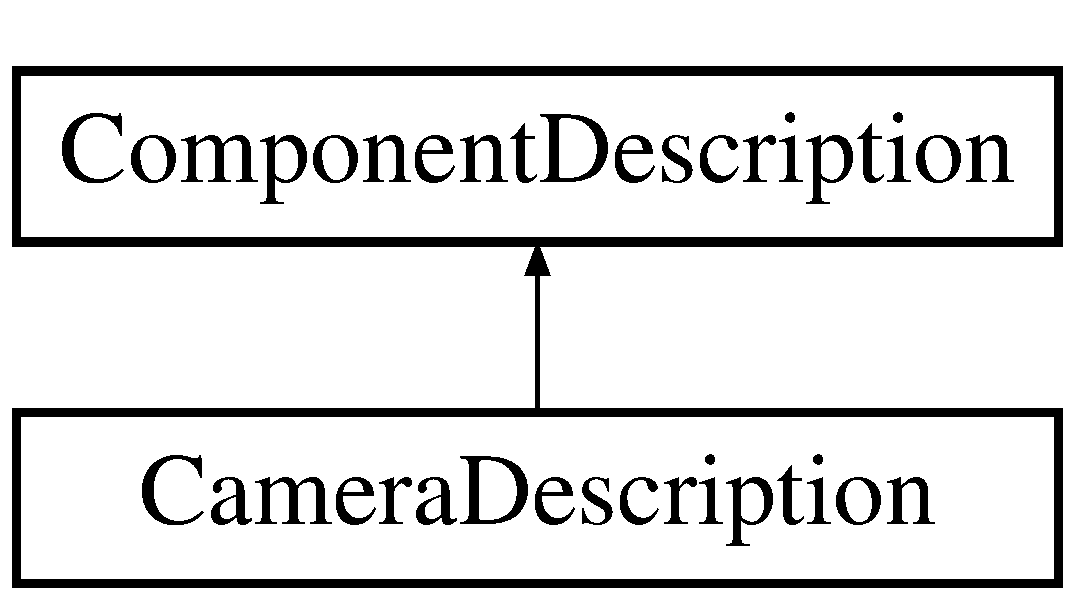
\includegraphics[height=2.000000cm]{class_camera_description}
\end{center}
\end{figure}
\subsection*{Public Member Functions}
\begin{DoxyCompactItemize}
\item 
\hypertarget{class_camera_description_a01634958c1db404fada946b45c96a71a}{}{\bfseries Camera\+Description} (float near, float far, float f, float r)\label{class_camera_description_a01634958c1db404fada946b45c96a71a}

\end{DoxyCompactItemize}
\subsection*{Public Attributes}
\begin{DoxyCompactItemize}
\item 
\hypertarget{class_camera_description_a3ac937ab778dd2826ee7321f14609070}{}float {\bfseries near\+Clip\+Plane}\label{class_camera_description_a3ac937ab778dd2826ee7321f14609070}

\item 
\hypertarget{class_camera_description_a8bc1d4022d6e3e5bbb8aa1f0081683b3}{}float {\bfseries far\+Clip\+Plane}\label{class_camera_description_a8bc1d4022d6e3e5bbb8aa1f0081683b3}

\item 
\hypertarget{class_camera_description_aed2916c3a9162b8727adb21633cdbe9b}{}float {\bfseries fov}\label{class_camera_description_aed2916c3a9162b8727adb21633cdbe9b}

\item 
\hypertarget{class_camera_description_a6e3da4e7ae4c3aa74ad6140061ea52e8}{}float {\bfseries ratio}\label{class_camera_description_a6e3da4e7ae4c3aa74ad6140061ea52e8}

\end{DoxyCompactItemize}


The documentation for this class was generated from the following file\+:\begin{DoxyCompactItemize}
\item 
/\+Users/guilherme\+\_\+cunha/\+Dev/\+G\+I\+T\+H\+U\+B/\+G\+U\+Inity/\+Source/Serialization\+Structs.\+hpp\end{DoxyCompactItemize}

\hypertarget{class_capsule_collider}{}\section{Capsule\+Collider Class Reference}
\label{class_capsule_collider}\index{Capsule\+Collider@{Capsule\+Collider}}


{\ttfamily \#include $<$Capsule\+Collider.\+hpp$>$}

Inheritance diagram for Capsule\+Collider\+:\begin{figure}[H]
\begin{center}
\leavevmode
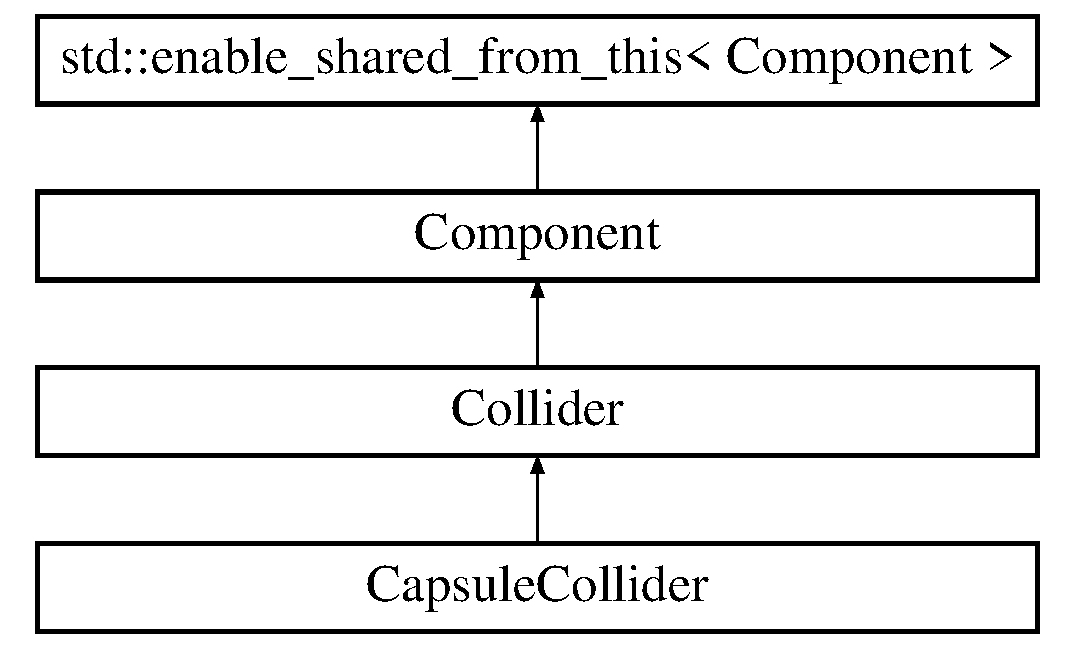
\includegraphics[height=4.000000cm]{class_capsule_collider}
\end{center}
\end{figure}
\subsection*{Public Member Functions}
\begin{DoxyCompactItemize}
\item 
\hyperlink{class_capsule_collider_a2f3f343173ed386673b045f8963246b0}{Capsule\+Collider} ()
\item 
\hyperlink{class_capsule_collider_a4d63d957812a224d7c476c75e76fd16f}{Capsule\+Collider} (Rotate\+Axis orientation, float half\+Height, float radius, Px\+Vec3 \hyperlink{class_collider_a42b57aa35ab665daf89ae844e479c560}{center})
\item 
\hyperlink{class_capsule_collider_ad0ea124fada29b0f3390cddb66b828a8}{$\sim$\+Capsule\+Collider} ()
\item 
void \hyperlink{class_capsule_collider_afeedbe30ba1eb78d1b8b1f0162f684d7}{set\+Orientation} (Rotate\+Axis orientation)
\item 
Rotate\+Axis \hyperlink{class_capsule_collider_a0c5a68adf4fab424ab878778dd6e4f9b}{get\+Orientation} ()
\item 
void \hyperlink{class_capsule_collider_a6304f7dea81fbb45a518e5052381d511}{set\+Height} (float height)
\item 
float \hyperlink{class_capsule_collider_a406bcbd57d22e9f6ad1626d2f4264a65}{get\+Height} ()
\item 
void \hyperlink{class_capsule_collider_aef1729d1b992406ab5daedfc7d03be9a}{set\+Radius} (float radius)
\item 
float \hyperlink{class_capsule_collider_a9e9013e8280c361033bf774dfea6d4e9}{get\+Radius} ()
\item 
virtual void \hyperlink{class_capsule_collider_a725516c53e2ac8eeee318107dc888163}{init} ()
\item 
virtual shared\+\_\+ptr$<$ \hyperlink{class_component}{Component} $>$ \hyperlink{class_capsule_collider_a6ee91020e9118a97f9d5960b088b7db7}{clone} () override
\item 
virtual shared\+\_\+ptr$<$ \hyperlink{class_component_description}{Component\+Description} $>$ \hyperlink{group__serialization__functions_ga9dc5198cfc2de557ac56210cce1dce82}{get\+Component\+Description} () override
\item 
virtual void \hyperlink{group__serialization__functions_ga6bd7fb4ea4628b29528aaf28d78ff325}{deserialize} (shared\+\_\+ptr$<$ \hyperlink{class_component_description}{Component\+Description} $>$ desc) override
\end{DoxyCompactItemize}
\subsection*{Additional Inherited Members}


\subsection{Detailed Description}
\hyperlink{class_capsule_collider}{Capsule\+Collider} is a volume collider with radius, height and orientation. Can either be real physics simulated or trigger only. 

\subsection{Constructor \& Destructor Documentation}
\hypertarget{class_capsule_collider_a2f3f343173ed386673b045f8963246b0}{}\index{Capsule\+Collider@{Capsule\+Collider}!Capsule\+Collider@{Capsule\+Collider}}
\index{Capsule\+Collider@{Capsule\+Collider}!Capsule\+Collider@{Capsule\+Collider}}
\subsubsection[{Capsule\+Collider()}]{\setlength{\rightskip}{0pt plus 5cm}Capsule\+Collider\+::\+Capsule\+Collider (
\begin{DoxyParamCaption}
{}
\end{DoxyParamCaption}
)}\label{class_capsule_collider_a2f3f343173ed386673b045f8963246b0}
Default Constructor \hypertarget{class_capsule_collider_a4d63d957812a224d7c476c75e76fd16f}{}\index{Capsule\+Collider@{Capsule\+Collider}!Capsule\+Collider@{Capsule\+Collider}}
\index{Capsule\+Collider@{Capsule\+Collider}!Capsule\+Collider@{Capsule\+Collider}}
\subsubsection[{Capsule\+Collider(\+Rotate\+Axis orientation, float half\+Height, float radius, Px\+Vec3 center)}]{\setlength{\rightskip}{0pt plus 5cm}Capsule\+Collider\+::\+Capsule\+Collider (
\begin{DoxyParamCaption}
\item[{Rotate\+Axis}]{orientation, }
\item[{float}]{half\+Height, }
\item[{float}]{radius, }
\item[{Px\+Vec3}]{center = {\ttfamily PxVec3(0,0,0)}}
\end{DoxyParamCaption}
)}\label{class_capsule_collider_a4d63d957812a224d7c476c75e76fd16f}
Deserialization Constructor \hypertarget{class_capsule_collider_ad0ea124fada29b0f3390cddb66b828a8}{}\index{Capsule\+Collider@{Capsule\+Collider}!````~Capsule\+Collider@{$\sim$\+Capsule\+Collider}}
\index{````~Capsule\+Collider@{$\sim$\+Capsule\+Collider}!Capsule\+Collider@{Capsule\+Collider}}
\subsubsection[{$\sim$\+Capsule\+Collider()}]{\setlength{\rightskip}{0pt plus 5cm}Capsule\+Collider\+::$\sim$\+Capsule\+Collider (
\begin{DoxyParamCaption}
{}
\end{DoxyParamCaption}
)}\label{class_capsule_collider_ad0ea124fada29b0f3390cddb66b828a8}
Default Destructor 

\subsection{Member Function Documentation}
\hypertarget{class_capsule_collider_a6ee91020e9118a97f9d5960b088b7db7}{}\index{Capsule\+Collider@{Capsule\+Collider}!clone@{clone}}
\index{clone@{clone}!Capsule\+Collider@{Capsule\+Collider}}
\subsubsection[{clone() override}]{\setlength{\rightskip}{0pt plus 5cm}shared\+\_\+ptr$<$ {\bf Component} $>$ Capsule\+Collider\+::clone (
\begin{DoxyParamCaption}
{}
\end{DoxyParamCaption}
)\hspace{0.3cm}{\ttfamily [override]}, {\ttfamily [virtual]}}\label{class_capsule_collider_a6ee91020e9118a97f9d5960b088b7db7}
Clones current component (Prototype Design Pattern) \begin{DoxyReturn}{Returns}
shared\+\_\+ptr to cloned \hyperlink{class_capsule_collider}{Capsule\+Collider} \hyperlink{class_component}{Component} 
\end{DoxyReturn}


Implements \hyperlink{class_collider_a28d0829db9804b27590afc9979e61a1c}{Collider}.

\hypertarget{class_capsule_collider_a406bcbd57d22e9f6ad1626d2f4264a65}{}\index{Capsule\+Collider@{Capsule\+Collider}!get\+Height@{get\+Height}}
\index{get\+Height@{get\+Height}!Capsule\+Collider@{Capsule\+Collider}}
\subsubsection[{get\+Height()}]{\setlength{\rightskip}{0pt plus 5cm}float Capsule\+Collider\+::get\+Height (
\begin{DoxyParamCaption}
{}
\end{DoxyParamCaption}
)}\label{class_capsule_collider_a406bcbd57d22e9f6ad1626d2f4264a65}
height Getter \hypertarget{class_capsule_collider_a0c5a68adf4fab424ab878778dd6e4f9b}{}\index{Capsule\+Collider@{Capsule\+Collider}!get\+Orientation@{get\+Orientation}}
\index{get\+Orientation@{get\+Orientation}!Capsule\+Collider@{Capsule\+Collider}}
\subsubsection[{get\+Orientation()}]{\setlength{\rightskip}{0pt plus 5cm}Rotate\+Axis Capsule\+Collider\+::get\+Orientation (
\begin{DoxyParamCaption}
{}
\end{DoxyParamCaption}
)}\label{class_capsule_collider_a0c5a68adf4fab424ab878778dd6e4f9b}
orientation Getter \hypertarget{class_capsule_collider_a9e9013e8280c361033bf774dfea6d4e9}{}\index{Capsule\+Collider@{Capsule\+Collider}!get\+Radius@{get\+Radius}}
\index{get\+Radius@{get\+Radius}!Capsule\+Collider@{Capsule\+Collider}}
\subsubsection[{get\+Radius()}]{\setlength{\rightskip}{0pt plus 5cm}float Capsule\+Collider\+::get\+Radius (
\begin{DoxyParamCaption}
{}
\end{DoxyParamCaption}
)}\label{class_capsule_collider_a9e9013e8280c361033bf774dfea6d4e9}
radius Getter \hypertarget{class_capsule_collider_a725516c53e2ac8eeee318107dc888163}{}\index{Capsule\+Collider@{Capsule\+Collider}!init@{init}}
\index{init@{init}!Capsule\+Collider@{Capsule\+Collider}}
\subsubsection[{init()}]{\setlength{\rightskip}{0pt plus 5cm}void Capsule\+Collider\+::init (
\begin{DoxyParamCaption}
{}
\end{DoxyParamCaption}
)\hspace{0.3cm}{\ttfamily [virtual]}}\label{class_capsule_collider_a725516c53e2ac8eeee318107dc888163}
\hyperlink{class_component}{Component} init override. Create a new Capsule Shape in the Phys\+X scene.

Init component override. Create a new Capsule Shape in the Phys\+X scene. 

Reimplemented from \hyperlink{class_collider_aed04ad82be15bcba1d3dc6a09f76dae6}{Collider}.

\hypertarget{class_capsule_collider_a6304f7dea81fbb45a518e5052381d511}{}\index{Capsule\+Collider@{Capsule\+Collider}!set\+Height@{set\+Height}}
\index{set\+Height@{set\+Height}!Capsule\+Collider@{Capsule\+Collider}}
\subsubsection[{set\+Height(float height)}]{\setlength{\rightskip}{0pt plus 5cm}void Capsule\+Collider\+::set\+Height (
\begin{DoxyParamCaption}
\item[{float}]{height}
\end{DoxyParamCaption}
)}\label{class_capsule_collider_a6304f7dea81fbb45a518e5052381d511}
height Setter \hypertarget{class_capsule_collider_afeedbe30ba1eb78d1b8b1f0162f684d7}{}\index{Capsule\+Collider@{Capsule\+Collider}!set\+Orientation@{set\+Orientation}}
\index{set\+Orientation@{set\+Orientation}!Capsule\+Collider@{Capsule\+Collider}}
\subsubsection[{set\+Orientation(\+Rotate\+Axis orientation)}]{\setlength{\rightskip}{0pt plus 5cm}void Capsule\+Collider\+::set\+Orientation (
\begin{DoxyParamCaption}
\item[{Rotate\+Axis}]{orientation}
\end{DoxyParamCaption}
)}\label{class_capsule_collider_afeedbe30ba1eb78d1b8b1f0162f684d7}
orientation Setter \hypertarget{class_capsule_collider_aef1729d1b992406ab5daedfc7d03be9a}{}\index{Capsule\+Collider@{Capsule\+Collider}!set\+Radius@{set\+Radius}}
\index{set\+Radius@{set\+Radius}!Capsule\+Collider@{Capsule\+Collider}}
\subsubsection[{set\+Radius(float radius)}]{\setlength{\rightskip}{0pt plus 5cm}void Capsule\+Collider\+::set\+Radius (
\begin{DoxyParamCaption}
\item[{float}]{radius}
\end{DoxyParamCaption}
)}\label{class_capsule_collider_aef1729d1b992406ab5daedfc7d03be9a}
radius Setter 

The documentation for this class was generated from the following files\+:\begin{DoxyCompactItemize}
\item 
/\+Users/guilherme\+\_\+cunha/\+Dev/\+G\+I\+T\+H\+U\+B/\+G\+U\+Inity/\+Source/Capsule\+Collider.\+hpp\item 
/\+Users/guilherme\+\_\+cunha/\+Dev/\+G\+I\+T\+H\+U\+B/\+G\+U\+Inity/\+Source/Capsule\+Collider.\+cpp\end{DoxyCompactItemize}

\hypertarget{class_capsule_collider_description}{}\section{Capsule\+Collider\+Description Class Reference}
\label{class_capsule_collider_description}\index{Capsule\+Collider\+Description@{Capsule\+Collider\+Description}}
Inheritance diagram for Capsule\+Collider\+Description\+:\begin{figure}[H]
\begin{center}
\leavevmode
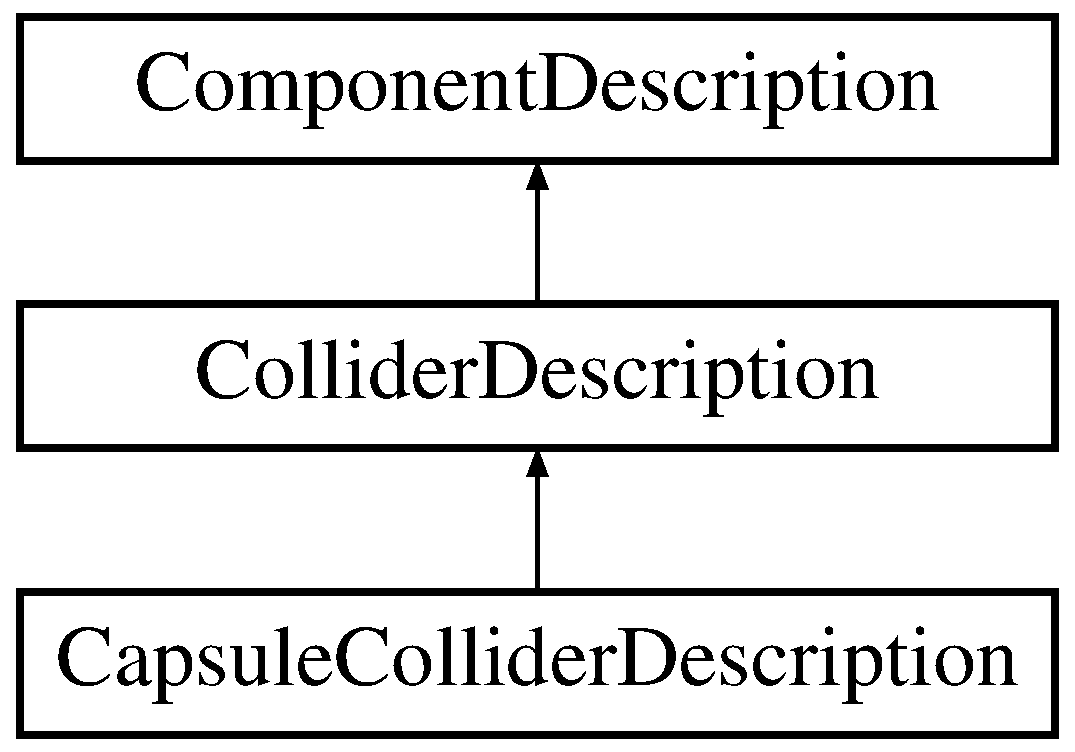
\includegraphics[height=3.000000cm]{class_capsule_collider_description}
\end{center}
\end{figure}
\subsection*{Public Member Functions}
\begin{DoxyCompactItemize}
\item 
\hypertarget{class_capsule_collider_description_a6f82452c0bf8074baf06ee2111e25e34}{}{\bfseries Capsule\+Collider\+Description} (float half\+H, float r, Rotate\+Axis o)\label{class_capsule_collider_description_a6f82452c0bf8074baf06ee2111e25e34}

\end{DoxyCompactItemize}
\subsection*{Public Attributes}
\begin{DoxyCompactItemize}
\item 
\hypertarget{class_capsule_collider_description_af13d45def5b1df197f2c86f32aad1e42}{}float {\bfseries radius}\label{class_capsule_collider_description_af13d45def5b1df197f2c86f32aad1e42}

\item 
\hypertarget{class_capsule_collider_description_a77ea825d23223c4b213a71bee6734622}{}float {\bfseries half\+Height}\label{class_capsule_collider_description_a77ea825d23223c4b213a71bee6734622}

\item 
\hypertarget{class_capsule_collider_description_af0de44deca178f669648f9de7dd271c7}{}Rotate\+Axis {\bfseries orientation}\label{class_capsule_collider_description_af0de44deca178f669648f9de7dd271c7}

\end{DoxyCompactItemize}


The documentation for this class was generated from the following file\+:\begin{DoxyCompactItemize}
\item 
/\+Users/guilherme\+\_\+cunha/\+Dev/\+G\+I\+T\+H\+U\+B/\+G\+U\+Inity/\+Source/Serialization\+Structs.\+hpp\end{DoxyCompactItemize}

\hypertarget{class_collider}{}\section{Collider Class Reference}
\label{class_collider}\index{Collider@{Collider}}


{\ttfamily \#include $<$Collider.\+hpp$>$}

Inheritance diagram for Collider\+:\begin{figure}[H]
\begin{center}
\leavevmode
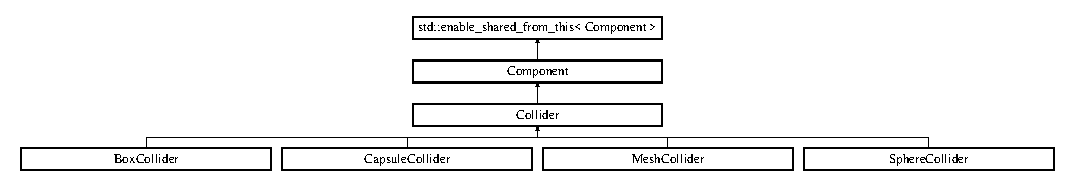
\includegraphics[height=2.066421cm]{class_collider}
\end{center}
\end{figure}
\subsection*{Public Member Functions}
\begin{DoxyCompactItemize}
\item 
\hyperlink{class_collider_aa7186870221f868bbc74c3ae8609fa66}{Collider} ()
\item 
virtual \hyperlink{class_collider_abf1ce43b287c870fd72918b023217a33}{$\sim$\+Collider} ()
\item 
void \hyperlink{class_collider_af96b9fde921e93d3072e49e0bfc1d942}{set\+Trigger} (bool \hyperlink{class_collider_a3068bd0bbdb66fc93a3ef3063ac556fa}{is\+Trigger})
\item 
bool \hyperlink{class_collider_ab5f78af93e01ca53d7a74820ff6c1537}{get\+Is\+Trigger} ()
\item 
void \hyperlink{class_collider_af023309d25aa50c66771bd0d804b1dea}{set\+Query\+Only} (bool \hyperlink{class_collider_a7a04883dc178bfc1b0bbf7750eb9f4d1}{is\+Query\+Only})
\item 
bool \hyperlink{class_collider_ac4bfad43c99e8e8897e55d28f7f84c3a}{get\+Query\+Only} ()
\item 
virtual void \hyperlink{class_collider_aed04ad82be15bcba1d3dc6a09f76dae6}{init} () override
\item 
virtual void \hyperlink{class_collider_a018ec33674acec77cbd18e4df9d8ad5b}{destroy} () override
\item 
virtual void \hyperlink{class_collider_ae29d151525174adbb950c15eafbf518e}{awake} () override
\item 
virtual void \hyperlink{class_collider_ade3d0403ff4c5429310adfbe41d889ee}{set\+Active} (bool \hyperlink{class_component_a6dad4f819c0814eee8219e9b391cf583}{is\+Active}) override
\item 
void \hyperlink{class_collider_a7ac3dc7291adfb3ea35c104fdebdf67a}{set\+Physics\+Material} (const shared\+\_\+ptr$<$ \hyperlink{class_physics_material}{Physics\+Material} $>$ phys\+Material)
\item 
shared\+\_\+ptr$<$ \hyperlink{class_physics_material}{Physics\+Material} $>$ \hyperlink{class_collider_adb62c0a8938b922c2b093511dcc12751}{get\+Physics\+Material} ()
\item 
virtual shared\+\_\+ptr$<$ \hyperlink{class_component}{Component} $>$ \hyperlink{class_collider_a28d0829db9804b27590afc9979e61a1c}{clone} () override=0
\item 
virtual shared\+\_\+ptr$<$ \hyperlink{class_component_description}{Component\+Description} $>$ \hyperlink{group__serialization__functions_ga9bee953be54c842bd37244d1f3126745}{get\+Component\+Description} () override=0
\item 
virtual void \hyperlink{group__serialization__functions_gaa82ff0f6d5986bf4128bc50ec9932a04}{deserialize} (shared\+\_\+ptr$<$ \hyperlink{class_component_description}{Component\+Description} $>$ desc) override=0
\end{DoxyCompactItemize}
\subsection*{Protected Attributes}
\begin{DoxyCompactItemize}
\item 
Px\+Vec3 \hyperlink{class_collider_a42b57aa35ab665daf89ae844e479c560}{center}
\item 
Px\+Shape $\ast$ \hyperlink{class_collider_a0eabd23889c23a5cb622547b1fc484d8}{shape}
\item 
shared\+\_\+ptr$<$ \hyperlink{class_physics_material}{Physics\+Material} $>$ \hyperlink{class_collider_a7cf889cd7bc213bcac3e0c6f5f42f150}{physics\+Material}
\item 
bool \hyperlink{class_collider_a3068bd0bbdb66fc93a3ef3063ac556fa}{is\+Trigger}
\item 
bool \hyperlink{class_collider_a7a04883dc178bfc1b0bbf7750eb9f4d1}{is\+Query\+Only}
\end{DoxyCompactItemize}
\subsection*{Additional Inherited Members}


\subsection{Detailed Description}
\hyperlink{class_collider}{Collider} is a component that adds either simulates real physics for an \hyperlink{class_actor}{Actor} or allows it to behave like a volume trigger. \hyperlink{class_collider}{Collider} is an abstract parent class for all the \hyperlink{class_collider}{Collider} types (\hyperlink{class_sphere_collider}{Sphere\+Collider}, \hyperlink{class_box_collider}{Box\+Collider}, \hyperlink{class_capsule_collider}{Capsule\+Collider} and \hyperlink{class_mesh_collider}{Mesh\+Collider}) 

\subsection{Constructor \& Destructor Documentation}
\hypertarget{class_collider_aa7186870221f868bbc74c3ae8609fa66}{}\index{Collider@{Collider}!Collider@{Collider}}
\index{Collider@{Collider}!Collider@{Collider}}
\subsubsection[{Collider()}]{\setlength{\rightskip}{0pt plus 5cm}Collider\+::\+Collider (
\begin{DoxyParamCaption}
{}
\end{DoxyParamCaption}
)\hspace{0.3cm}{\ttfamily [inline]}}\label{class_collider_aa7186870221f868bbc74c3ae8609fa66}
Default Constructor \hypertarget{class_collider_abf1ce43b287c870fd72918b023217a33}{}\index{Collider@{Collider}!````~Collider@{$\sim$\+Collider}}
\index{````~Collider@{$\sim$\+Collider}!Collider@{Collider}}
\subsubsection[{$\sim$\+Collider()}]{\setlength{\rightskip}{0pt plus 5cm}virtual Collider\+::$\sim$\+Collider (
\begin{DoxyParamCaption}
{}
\end{DoxyParamCaption}
)\hspace{0.3cm}{\ttfamily [inline]}, {\ttfamily [virtual]}}\label{class_collider_abf1ce43b287c870fd72918b023217a33}
Default Destructor. Virtual because it\textquotesingle{}s parent class 

\subsection{Member Function Documentation}
\hypertarget{class_collider_ae29d151525174adbb950c15eafbf518e}{}\index{Collider@{Collider}!awake@{awake}}
\index{awake@{awake}!Collider@{Collider}}
\subsubsection[{awake() override}]{\setlength{\rightskip}{0pt plus 5cm}virtual void Collider\+::awake (
\begin{DoxyParamCaption}
{}
\end{DoxyParamCaption}
)\hspace{0.3cm}{\ttfamily [inline]}, {\ttfamily [override]}, {\ttfamily [virtual]}}\label{class_collider_ae29d151525174adbb950c15eafbf518e}
\hyperlink{class_component}{Component} awake override 

Reimplemented from \hyperlink{class_component_ae413974ecdbc8f65c6ff707b84278b0e}{Component}.

\hypertarget{class_collider_a28d0829db9804b27590afc9979e61a1c}{}\index{Collider@{Collider}!clone@{clone}}
\index{clone@{clone}!Collider@{Collider}}
\subsubsection[{clone() override=0}]{\setlength{\rightskip}{0pt plus 5cm}virtual shared\+\_\+ptr$<${\bf Component}$>$ Collider\+::clone (
\begin{DoxyParamCaption}
{}
\end{DoxyParamCaption}
)\hspace{0.3cm}{\ttfamily [override]}, {\ttfamily [pure virtual]}}\label{class_collider_a28d0829db9804b27590afc9979e61a1c}
Pure virtual function. Clones current component (Prototype Design Pattern) \begin{DoxyReturn}{Returns}
shared\+\_\+ptr to cloned \hyperlink{class_collider}{Collider} \hyperlink{class_component}{Component} 
\end{DoxyReturn}


Implements \hyperlink{class_component_a74c984bd819bbef16fd4f306a90d34fe}{Component}.



Implemented in \hyperlink{class_capsule_collider_a6ee91020e9118a97f9d5960b088b7db7}{Capsule\+Collider}, \hyperlink{class_sphere_collider_a68cd4eaf4ee2b13ac48efc38a760ff36}{Sphere\+Collider}, \hyperlink{class_box_collider_ab9154438078b0fb9d33f2f8958e3a71e}{Box\+Collider}, and \hyperlink{class_mesh_collider_a9965a490a1e945858dd9f1601b239878}{Mesh\+Collider}.

\hypertarget{class_collider_a018ec33674acec77cbd18e4df9d8ad5b}{}\index{Collider@{Collider}!destroy@{destroy}}
\index{destroy@{destroy}!Collider@{Collider}}
\subsubsection[{destroy() override}]{\setlength{\rightskip}{0pt plus 5cm}void Collider\+::destroy (
\begin{DoxyParamCaption}
{}
\end{DoxyParamCaption}
)\hspace{0.3cm}{\ttfamily [override]}, {\ttfamily [virtual]}}\label{class_collider_a018ec33674acec77cbd18e4df9d8ad5b}
\hyperlink{class_component}{Component} destroy override 

Reimplemented from \hyperlink{class_component_a77b8fff56ddce5dd0b4a9dabb0b5202b}{Component}.

\hypertarget{class_collider_ab5f78af93e01ca53d7a74820ff6c1537}{}\index{Collider@{Collider}!get\+Is\+Trigger@{get\+Is\+Trigger}}
\index{get\+Is\+Trigger@{get\+Is\+Trigger}!Collider@{Collider}}
\subsubsection[{get\+Is\+Trigger()}]{\setlength{\rightskip}{0pt plus 5cm}bool Collider\+::get\+Is\+Trigger (
\begin{DoxyParamCaption}
{}
\end{DoxyParamCaption}
)}\label{class_collider_ab5f78af93e01ca53d7a74820ff6c1537}
is\+Trigger getter \begin{DoxyReturn}{Returns}
true if it\textquotesingle{}s just a trigger, false if it physics simulated 
\end{DoxyReturn}
\hypertarget{class_collider_adb62c0a8938b922c2b093511dcc12751}{}\index{Collider@{Collider}!get\+Physics\+Material@{get\+Physics\+Material}}
\index{get\+Physics\+Material@{get\+Physics\+Material}!Collider@{Collider}}
\subsubsection[{get\+Physics\+Material()}]{\setlength{\rightskip}{0pt plus 5cm}shared\+\_\+ptr$<$ {\bf Physics\+Material} $>$ Collider\+::get\+Physics\+Material (
\begin{DoxyParamCaption}
{}
\end{DoxyParamCaption}
)}\label{class_collider_adb62c0a8938b922c2b093511dcc12751}
physics\+Material getter \begin{DoxyReturn}{Returns}
referente to \hyperlink{class_physics_material}{Physics\+Material} 
\end{DoxyReturn}
\hypertarget{class_collider_ac4bfad43c99e8e8897e55d28f7f84c3a}{}\index{Collider@{Collider}!get\+Query\+Only@{get\+Query\+Only}}
\index{get\+Query\+Only@{get\+Query\+Only}!Collider@{Collider}}
\subsubsection[{get\+Query\+Only()}]{\setlength{\rightskip}{0pt plus 5cm}bool Collider\+::get\+Query\+Only (
\begin{DoxyParamCaption}
{}
\end{DoxyParamCaption}
)}\label{class_collider_ac4bfad43c99e8e8897e55d28f7f84c3a}
is\+Query\+Only getter \begin{DoxyReturn}{Returns}
true if this object is only used in queries, false otherwise
\end{DoxyReturn}
is\+Query\+Only getter 
\begin{DoxyParams}[1]{Parameters}
\mbox{\tt in}  & {\em query\+Only} & true if this object is only used in queries, false otherwise \\
\hline
\end{DoxyParams}
\hypertarget{class_collider_aed04ad82be15bcba1d3dc6a09f76dae6}{}\index{Collider@{Collider}!init@{init}}
\index{init@{init}!Collider@{Collider}}
\subsubsection[{init() override}]{\setlength{\rightskip}{0pt plus 5cm}void Collider\+::init (
\begin{DoxyParamCaption}
{}
\end{DoxyParamCaption}
)\hspace{0.3cm}{\ttfamily [override]}, {\ttfamily [virtual]}}\label{class_collider_aed04ad82be15bcba1d3dc6a09f76dae6}
\hyperlink{class_component}{Component} init override

\hyperlink{class_component}{Component} Init override 

Reimplemented from \hyperlink{class_component_a162f8cdc070537a71f2ad0b5e763b86f}{Component}.



Reimplemented in \hyperlink{class_capsule_collider_a725516c53e2ac8eeee318107dc888163}{Capsule\+Collider}, \hyperlink{class_sphere_collider_aa51773fa54349bec5730b3ae528c4179}{Sphere\+Collider}, \hyperlink{class_box_collider_ad98ff62ff6b5c48dc8f18b1a2d2429e4}{Box\+Collider}, and \hyperlink{class_mesh_collider_ac906075dfa0f6ea801d82738c4b09231}{Mesh\+Collider}.

\hypertarget{class_collider_ade3d0403ff4c5429310adfbe41d889ee}{}\index{Collider@{Collider}!set\+Active@{set\+Active}}
\index{set\+Active@{set\+Active}!Collider@{Collider}}
\subsubsection[{set\+Active(bool is\+Active) override}]{\setlength{\rightskip}{0pt plus 5cm}void Collider\+::set\+Active (
\begin{DoxyParamCaption}
\item[{bool}]{is\+Active}
\end{DoxyParamCaption}
)\hspace{0.3cm}{\ttfamily [override]}, {\ttfamily [virtual]}}\label{class_collider_ade3d0403ff4c5429310adfbe41d889ee}
\hyperlink{class_component}{Component} set\+Active override. Changes Phys\+X settings

\hyperlink{class_component}{Component} set\+Active override 

Reimplemented from \hyperlink{class_component}{Component}.

\hypertarget{class_collider_a7ac3dc7291adfb3ea35c104fdebdf67a}{}\index{Collider@{Collider}!set\+Physics\+Material@{set\+Physics\+Material}}
\index{set\+Physics\+Material@{set\+Physics\+Material}!Collider@{Collider}}
\subsubsection[{set\+Physics\+Material(const shared\+\_\+ptr$<$ Physics\+Material $>$ phys\+Material)}]{\setlength{\rightskip}{0pt plus 5cm}void Collider\+::set\+Physics\+Material (
\begin{DoxyParamCaption}
\item[{const shared\+\_\+ptr$<$ {\bf Physics\+Material} $>$}]{phys\+Material}
\end{DoxyParamCaption}
)}\label{class_collider_a7ac3dc7291adfb3ea35c104fdebdf67a}
physics\+Material getter 
\begin{DoxyParams}[1]{Parameters}
\mbox{\tt in}  & {\em reference} & to \hyperlink{class_physics_material}{Physics\+Material} \\
\hline
\end{DoxyParams}
\hypertarget{class_collider_af023309d25aa50c66771bd0d804b1dea}{}\index{Collider@{Collider}!set\+Query\+Only@{set\+Query\+Only}}
\index{set\+Query\+Only@{set\+Query\+Only}!Collider@{Collider}}
\subsubsection[{set\+Query\+Only(bool is\+Query\+Only)}]{\setlength{\rightskip}{0pt plus 5cm}void Collider\+::set\+Query\+Only (
\begin{DoxyParamCaption}
\item[{bool}]{is\+Query\+Only}
\end{DoxyParamCaption}
)}\label{class_collider_af023309d25aa50c66771bd0d804b1dea}
is\+Query\+Only getter 
\begin{DoxyParams}[1]{Parameters}
\mbox{\tt in}  & {\em query\+Only} & true if this object is only used in queries, false otherwise\\
\hline
\end{DoxyParams}
is\+Query\+Only getter \begin{DoxyReturn}{Returns}
true if this object is only used in queries, false otherwise 
\end{DoxyReturn}
\hypertarget{class_collider_af96b9fde921e93d3072e49e0bfc1d942}{}\index{Collider@{Collider}!set\+Trigger@{set\+Trigger}}
\index{set\+Trigger@{set\+Trigger}!Collider@{Collider}}
\subsubsection[{set\+Trigger(bool is\+Trigger)}]{\setlength{\rightskip}{0pt plus 5cm}void Collider\+::set\+Trigger (
\begin{DoxyParamCaption}
\item[{bool}]{is\+Trigger}
\end{DoxyParamCaption}
)}\label{class_collider_af96b9fde921e93d3072e49e0bfc1d942}
is\+Trigger setter 
\begin{DoxyParams}[1]{Parameters}
\mbox{\tt in}  & {\em is\+Trigger} & -\/ true if it\textquotesingle{}s just a trigger, false if it physics simulated \\
\hline
\end{DoxyParams}


\subsection{Member Data Documentation}
\hypertarget{class_collider_a42b57aa35ab665daf89ae844e479c560}{}\index{Collider@{Collider}!center@{center}}
\index{center@{center}!Collider@{Collider}}
\subsubsection[{center}]{\setlength{\rightskip}{0pt plus 5cm}Px\+Vec3 Collider\+::center\hspace{0.3cm}{\ttfamily [protected]}}\label{class_collider_a42b57aa35ab665daf89ae844e479c560}
The center of the collider \hypertarget{class_collider_a7a04883dc178bfc1b0bbf7750eb9f4d1}{}\index{Collider@{Collider}!is\+Query\+Only@{is\+Query\+Only}}
\index{is\+Query\+Only@{is\+Query\+Only}!Collider@{Collider}}
\subsubsection[{is\+Query\+Only}]{\setlength{\rightskip}{0pt plus 5cm}bool Collider\+::is\+Query\+Only\hspace{0.3cm}{\ttfamily [protected]}}\label{class_collider_a7a04883dc178bfc1b0bbf7750eb9f4d1}
Is this collider used for queries only? \hypertarget{class_collider_a3068bd0bbdb66fc93a3ef3063ac556fa}{}\index{Collider@{Collider}!is\+Trigger@{is\+Trigger}}
\index{is\+Trigger@{is\+Trigger}!Collider@{Collider}}
\subsubsection[{is\+Trigger}]{\setlength{\rightskip}{0pt plus 5cm}bool Collider\+::is\+Trigger\hspace{0.3cm}{\ttfamily [protected]}}\label{class_collider_a3068bd0bbdb66fc93a3ef3063ac556fa}
Is this collider a trigger or should it simulate real world physics? \hypertarget{class_collider_a7cf889cd7bc213bcac3e0c6f5f42f150}{}\index{Collider@{Collider}!physics\+Material@{physics\+Material}}
\index{physics\+Material@{physics\+Material}!Collider@{Collider}}
\subsubsection[{physics\+Material}]{\setlength{\rightskip}{0pt plus 5cm}shared\+\_\+ptr$<${\bf Physics\+Material}$>$ Collider\+::physics\+Material\hspace{0.3cm}{\ttfamily [protected]}}\label{class_collider_a7cf889cd7bc213bcac3e0c6f5f42f150}
The physics material that determines the behaviour of the physics shape \hypertarget{class_collider_a0eabd23889c23a5cb622547b1fc484d8}{}\index{Collider@{Collider}!shape@{shape}}
\index{shape@{shape}!Collider@{Collider}}
\subsubsection[{shape}]{\setlength{\rightskip}{0pt plus 5cm}Px\+Shape$\ast$ Collider\+::shape\hspace{0.3cm}{\ttfamily [protected]}}\label{class_collider_a0eabd23889c23a5cb622547b1fc484d8}
The Phys\+X Shape of the collider 

The documentation for this class was generated from the following files\+:\begin{DoxyCompactItemize}
\item 
/\+Users/guilherme\+\_\+cunha/\+Dev/\+G\+I\+T\+H\+U\+B/\+G\+U\+Inity/\+Source/Collider.\+hpp\item 
/\+Users/guilherme\+\_\+cunha/\+Dev/\+G\+I\+T\+H\+U\+B/\+G\+U\+Inity/\+Source/Collider.\+cpp\end{DoxyCompactItemize}

\hypertarget{class_collider_description}{}\section{Collider\+Description Class Reference}
\label{class_collider_description}\index{Collider\+Description@{Collider\+Description}}
Inheritance diagram for Collider\+Description\+:\begin{figure}[H]
\begin{center}
\leavevmode
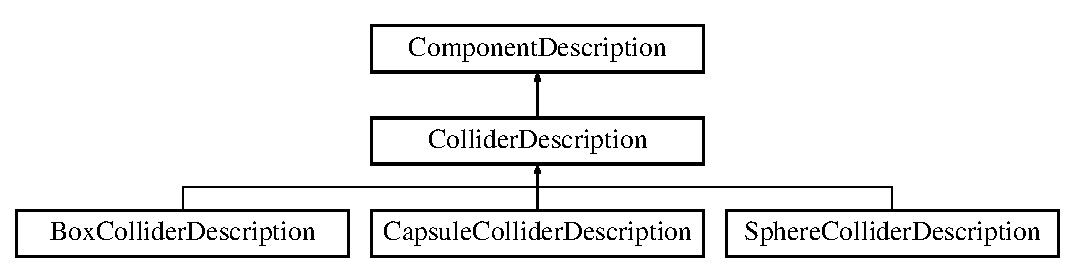
\includegraphics[height=3.000000cm]{class_collider_description}
\end{center}
\end{figure}
\subsection*{Public Attributes}
\begin{DoxyCompactItemize}
\item 
\hypertarget{class_collider_description_a424117a32221edd34084671567d8a0e4}{}Px\+Vec3 {\bfseries center}\label{class_collider_description_a424117a32221edd34084671567d8a0e4}

\end{DoxyCompactItemize}


The documentation for this class was generated from the following file\+:\begin{DoxyCompactItemize}
\item 
/\+Users/guilherme\+\_\+cunha/\+Dev/\+G\+I\+T\+H\+U\+B/\+G\+U\+Inity/\+Source/Serialization\+Structs.\+hpp\end{DoxyCompactItemize}

\hypertarget{class_component}{}\section{Component Class Reference}
\label{class_component}\index{Component@{Component}}


{\ttfamily \#include $<$Component.\+hpp$>$}

Inheritance diagram for Component\+:\begin{figure}[H]
\begin{center}
\leavevmode
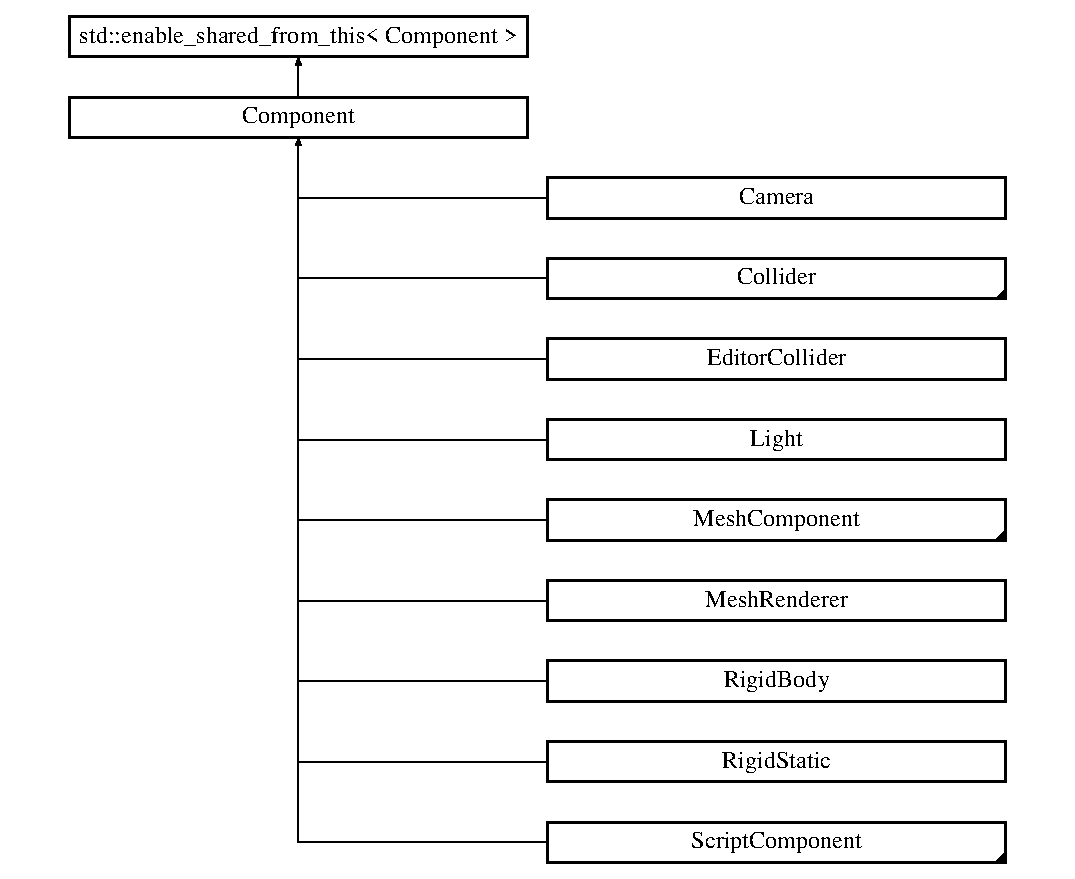
\includegraphics[height=11.000000cm]{class_component}
\end{center}
\end{figure}
\subsection*{Public Member Functions}
\begin{DoxyCompactItemize}
\item 
\hyperlink{class_component_a8775db6d1a2c1afc2e77cd3c8f39da6f}{Component} ()
\item 
virtual \hyperlink{class_component_ab8378fa275af98e568a7e91d33d867af}{$\sim$\+Component} ()
\item 
virtual void \hyperlink{class_component_a162f8cdc070537a71f2ad0b5e763b86f}{init} ()
\item 
virtual void \hyperlink{class_component_a77b8fff56ddce5dd0b4a9dabb0b5202b}{destroy} ()
\item 
\hypertarget{class_component_a8dcaa1d0ec8d0fbceca41cad03905ff2}{}virtual void {\bfseries set\+Active} (bool \hyperlink{class_component_a6dad4f819c0814eee8219e9b391cf583}{is\+Active})\label{class_component_a8dcaa1d0ec8d0fbceca41cad03905ff2}

\item 
virtual void \hyperlink{class_component_ae413974ecdbc8f65c6ff707b84278b0e}{awake} ()
\item 
virtual void \hyperlink{class_component_a72d67b02e6733c1a6fb73cbaaf8ebff4}{tick} (float delta\+Secods)
\item 
shared\+\_\+ptr$<$ \hyperlink{class_actor}{Actor} $>$ \hyperlink{class_component_a1c8bf7d2a699782d46fef1c1860ef23e}{get\+Actor} ()
\item 
void \hyperlink{class_component_a2115d06bfdbe42793fb750b5c4659ac3}{set\+Actor} (weak\+\_\+ptr$<$ \hyperlink{class_actor}{Actor} $>$ actor)
\item 
virtual shared\+\_\+ptr$<$ \hyperlink{class_component}{Component} $>$ \hyperlink{class_component_a74c984bd819bbef16fd4f306a90d34fe}{clone} ()=0
\item 
virtual shared\+\_\+ptr$<$ \hyperlink{class_component_description}{Component\+Description} $>$ \hyperlink{group__serialization__functions_gad6dca56c78283c5a036496ce8d386523}{get\+Component\+Description} ()=0
\item 
virtual void \hyperlink{group__serialization__functions_ga86158de289c38ea2b518043e1bb63f53}{deserialize} (shared\+\_\+ptr$<$ \hyperlink{class_component_description}{Component\+Description} $>$ desc)=0
\end{DoxyCompactItemize}
\subsection*{Protected Member Functions}
\begin{DoxyCompactItemize}
\item 
void \hyperlink{class_component_a1751659f91953e2452f2b45f034b3dea}{set\+Copy\+Mode} (bool \hyperlink{class_component_aab9de8ee5f46e5cc42607bb9243ccd6d}{init\+With\+Data})
\end{DoxyCompactItemize}
\subsection*{Protected Attributes}
\begin{DoxyCompactItemize}
\item 
bool \hyperlink{class_component_aab9de8ee5f46e5cc42607bb9243ccd6d}{init\+With\+Data}
\item 
bool \hyperlink{class_component_a6dad4f819c0814eee8219e9b391cf583}{is\+Active}
\end{DoxyCompactItemize}


\subsection{Detailed Description}
\hyperlink{class_component}{Component} is the very basis of the engine. All the actor behaviour should come from a component Component-\/based game engines allow for small, modular classes that are reused very often. \hyperlink{class_component}{Component} behaviour can vary from custom \hyperlink{class_script_component}{Script\+Component} (custom behaviour) to \hyperlink{class_rigid_body}{Rigid\+Body} physics and \hyperlink{class_mesh_renderer}{Mesh\+Renderer}. A \hyperlink{class_component}{Component} can only exist in conjunction with an actor. \hyperlink{class_component}{Component} is an abstract class and is the parent of all Components. 

\subsection{Constructor \& Destructor Documentation}
\hypertarget{class_component_a8775db6d1a2c1afc2e77cd3c8f39da6f}{}\index{Component@{Component}!Component@{Component}}
\index{Component@{Component}!Component@{Component}}
\subsubsection[{Component()}]{\setlength{\rightskip}{0pt plus 5cm}Component\+::\+Component (
\begin{DoxyParamCaption}
{}
\end{DoxyParamCaption}
)}\label{class_component_a8775db6d1a2c1afc2e77cd3c8f39da6f}
Default Constructor \hypertarget{class_component_ab8378fa275af98e568a7e91d33d867af}{}\index{Component@{Component}!````~Component@{$\sim$\+Component}}
\index{````~Component@{$\sim$\+Component}!Component@{Component}}
\subsubsection[{$\sim$\+Component()}]{\setlength{\rightskip}{0pt plus 5cm}Component\+::$\sim$\+Component (
\begin{DoxyParamCaption}
{}
\end{DoxyParamCaption}
)\hspace{0.3cm}{\ttfamily [virtual]}}\label{class_component_ab8378fa275af98e568a7e91d33d867af}
Default Destructor. Virtual because is parent class 

\subsection{Member Function Documentation}
\hypertarget{class_component_ae413974ecdbc8f65c6ff707b84278b0e}{}\index{Component@{Component}!awake@{awake}}
\index{awake@{awake}!Component@{Component}}
\subsubsection[{awake()}]{\setlength{\rightskip}{0pt plus 5cm}virtual void Component\+::awake (
\begin{DoxyParamCaption}
{}
\end{DoxyParamCaption}
)\hspace{0.3cm}{\ttfamily [inline]}, {\ttfamily [virtual]}}\label{class_component_ae413974ecdbc8f65c6ff707b84278b0e}
Called by \hyperlink{class_actor}{Actor} owner when it\textquotesingle{}s first awaken 

Reimplemented in \hyperlink{class_camera_adec93b934ee03e786a949fbc2b9d169e}{Camera}, \hyperlink{class_collider_ae29d151525174adbb950c15eafbf518e}{Collider}, \hyperlink{class_script_component_a4667b8a3712e18b25cd6f49f12c5677d}{Script\+Component}, \hyperlink{class_scale_tool_abd0df3bb4452336ac89b914968b91f39}{Scale\+Tool}, \hyperlink{class_player_script_acb623eb7cdcfc49b7848bf7d60809cb7}{Player\+Script}, \hyperlink{class_move_tool_ac53066bdb36f2e01234fa58a20cc1f0d}{Move\+Tool}, \hyperlink{class_rotate_handle_a93caa7dd2992d5dc3fcef9cbc4278bed}{Rotate\+Handle}, \hyperlink{class_rotate_tool_af476de7866d44808efd35fe431710049}{Rotate\+Tool}, and \hyperlink{class_increase_collider_script_a2a3291f10ec9cd908a0c45992847d7fe}{Increase\+Collider\+Script}.

\hypertarget{class_component_a74c984bd819bbef16fd4f306a90d34fe}{}\index{Component@{Component}!clone@{clone}}
\index{clone@{clone}!Component@{Component}}
\subsubsection[{clone()=0}]{\setlength{\rightskip}{0pt plus 5cm}virtual shared\+\_\+ptr$<${\bf Component}$>$ Component\+::clone (
\begin{DoxyParamCaption}
{}
\end{DoxyParamCaption}
)\hspace{0.3cm}{\ttfamily [pure virtual]}}\label{class_component_a74c984bd819bbef16fd4f306a90d34fe}
Pure virtual function. Clones current component (Prototype Design Pattern) \begin{DoxyReturn}{Returns}
shared\+\_\+ptr to cloned \hyperlink{class_component}{Component} 
\end{DoxyReturn}


Implemented in \hyperlink{class_camera_a0d6043b74adb8fc9d8f8aaa66ea19aa3}{Camera}, \hyperlink{class_rigid_body_a7acbed507a6deb5d83d381251ba224a8}{Rigid\+Body}, \hyperlink{class_collider_a28d0829db9804b27590afc9979e61a1c}{Collider}, \hyperlink{class_mesh_renderer_a78a5a5b66bb12c2b50f5356292afd93a}{Mesh\+Renderer}, \hyperlink{class_capsule_collider_a6ee91020e9118a97f9d5960b088b7db7}{Capsule\+Collider}, \hyperlink{class_font_mesh_a4dd3900fcbb33aca326d1cd1871e7b92}{Font\+Mesh}, \hyperlink{class_script_component_adebdf5187e8f41f68f445ff7555d5036}{Script\+Component}, \hyperlink{class_editor_collider_abfee383f62b5bc06afffe5beedb729e3}{Editor\+Collider}, \hyperlink{class_light_ae8747116c592100394c89f76035725e5}{Light}, \hyperlink{class_mesh_component_ace2f1acdce65f1c37b56a5b3ef507e8d}{Mesh\+Component}, \hyperlink{class_player_script_a75a83f06a2acb93ce1a629dcf2dabf5c}{Player\+Script}, \hyperlink{class_rigid_static_a5fef27a8ca3f6e969fb4c8312c1bba0a}{Rigid\+Static}, \hyperlink{class_sphere_collider_a68cd4eaf4ee2b13ac48efc38a760ff36}{Sphere\+Collider}, \hyperlink{class_box_collider_ab9154438078b0fb9d33f2f8958e3a71e}{Box\+Collider}, \hyperlink{class_mesh_filter_a6645cf7989fad04e40096955296b96a2}{Mesh\+Filter}, and \hyperlink{class_mesh_collider_a9965a490a1e945858dd9f1601b239878}{Mesh\+Collider}.

\hypertarget{class_component_a77b8fff56ddce5dd0b4a9dabb0b5202b}{}\index{Component@{Component}!destroy@{destroy}}
\index{destroy@{destroy}!Component@{Component}}
\subsubsection[{destroy()}]{\setlength{\rightskip}{0pt plus 5cm}virtual void Component\+::destroy (
\begin{DoxyParamCaption}
{}
\end{DoxyParamCaption}
)\hspace{0.3cm}{\ttfamily [inline]}, {\ttfamily [virtual]}}\label{class_component_a77b8fff56ddce5dd0b4a9dabb0b5202b}
Destroys \hyperlink{class_component}{Component} and release any component-\/specific members 

Reimplemented in \hyperlink{class_camera_a994622d61d20af75b2e86f5e39b01299}{Camera}, \hyperlink{class_collider_a018ec33674acec77cbd18e4df9d8ad5b}{Collider}, \hyperlink{class_mesh_renderer_acb0c4dc40c30d70157adb51612e08013}{Mesh\+Renderer}, \hyperlink{class_rigid_body_a5ceba4a769ea558e5c7efd472e822248}{Rigid\+Body}, \hyperlink{class_light_a5068d4a5fa02cd63a693030dc4a359fe}{Light}, \hyperlink{class_script_component_a3e7c2770a1ee8bcc1fd8d39fdb65cc44}{Script\+Component}, and \hyperlink{class_rigid_static_abd99e84cc884043d5afde1b95fb0d3b3}{Rigid\+Static}.

\hypertarget{class_component_a1c8bf7d2a699782d46fef1c1860ef23e}{}\index{Component@{Component}!get\+Actor@{get\+Actor}}
\index{get\+Actor@{get\+Actor}!Component@{Component}}
\subsubsection[{get\+Actor()}]{\setlength{\rightskip}{0pt plus 5cm}shared\+\_\+ptr$<$ {\bf Actor} $>$ Component\+::get\+Actor (
\begin{DoxyParamCaption}
{}
\end{DoxyParamCaption}
)}\label{class_component_a1c8bf7d2a699782d46fef1c1860ef23e}
Getter for owner \hyperlink{class_actor}{Actor} \begin{DoxyReturn}{Returns}
shared\+\_\+ptr for the owner 
\end{DoxyReturn}
\hypertarget{class_component_a162f8cdc070537a71f2ad0b5e763b86f}{}\index{Component@{Component}!init@{init}}
\index{init@{init}!Component@{Component}}
\subsubsection[{init()}]{\setlength{\rightskip}{0pt plus 5cm}virtual void Component\+::init (
\begin{DoxyParamCaption}
{}
\end{DoxyParamCaption}
)\hspace{0.3cm}{\ttfamily [inline]}, {\ttfamily [virtual]}}\label{class_component_a162f8cdc070537a71f2ad0b5e763b86f}
Initializes the component. Initialization should not be done in constructor due to enable\+\_\+shared\+\_\+from\+\_\+this$<$\+T$>$ inheritance. 

Reimplemented in \hyperlink{class_camera_aa575c1bbde6ae31425e233f0204af38c}{Camera}, \hyperlink{class_collider_aed04ad82be15bcba1d3dc6a09f76dae6}{Collider}, \hyperlink{class_capsule_collider_a725516c53e2ac8eeee318107dc888163}{Capsule\+Collider}, \hyperlink{class_mesh_renderer_ae77ac8e3b28e1890771860d5726fe043}{Mesh\+Renderer}, \hyperlink{class_rigid_body_aa419718573cb8042c3c7cbe671d69c4c}{Rigid\+Body}, \hyperlink{class_light_a2c59296fb881070f1e7064ec3ccd4d3d}{Light}, \hyperlink{class_sphere_collider_aa51773fa54349bec5730b3ae528c4179}{Sphere\+Collider}, \hyperlink{class_editor_collider_a6581dd66dd2881b0faafe6975b4a188c}{Editor\+Collider}, \hyperlink{class_script_component_a6fb8a859ed628b7b97801a2b3fb4f8ea}{Script\+Component}, \hyperlink{class_rigid_static_a2844109f1ef8fe36a25ce065934d703c}{Rigid\+Static}, \hyperlink{class_box_collider_ad98ff62ff6b5c48dc8f18b1a2d2429e4}{Box\+Collider}, \hyperlink{class_mesh_collider_ac906075dfa0f6ea801d82738c4b09231}{Mesh\+Collider}, and \hyperlink{class_editor_camera_control_af672d52ea342e6762f9f104898959181}{Editor\+Camera\+Control}.

\hypertarget{class_component_a2115d06bfdbe42793fb750b5c4659ac3}{}\index{Component@{Component}!set\+Actor@{set\+Actor}}
\index{set\+Actor@{set\+Actor}!Component@{Component}}
\subsubsection[{set\+Actor(weak\+\_\+ptr$<$ Actor $>$ actor)}]{\setlength{\rightskip}{0pt plus 5cm}void Component\+::set\+Actor (
\begin{DoxyParamCaption}
\item[{weak\+\_\+ptr$<$ {\bf Actor} $>$}]{actor}
\end{DoxyParamCaption}
)}\label{class_component_a2115d06bfdbe42793fb750b5c4659ac3}
Setter for owner \hyperlink{class_actor}{Actor} 
\begin{DoxyParams}{Parameters}
{\em owner} & \hyperlink{class_actor}{Actor} \\
\hline
\end{DoxyParams}
\hypertarget{class_component_a1751659f91953e2452f2b45f034b3dea}{}\index{Component@{Component}!set\+Copy\+Mode@{set\+Copy\+Mode}}
\index{set\+Copy\+Mode@{set\+Copy\+Mode}!Component@{Component}}
\subsubsection[{set\+Copy\+Mode(bool init\+With\+Data)}]{\setlength{\rightskip}{0pt plus 5cm}void Component\+::set\+Copy\+Mode (
\begin{DoxyParamCaption}
\item[{bool}]{init\+With\+Data}
\end{DoxyParamCaption}
)\hspace{0.3cm}{\ttfamily [protected]}}\label{class_component_a1751659f91953e2452f2b45f034b3dea}
Used when been deserialized or cloned 
\begin{DoxyParams}[1]{Parameters}
\mbox{\tt in}  & {\em init\+With\+Data} & true if this component data will come from clone of deserialization, false if it\textquotesingle{}s a new component being creates \\
\hline
\end{DoxyParams}
\hypertarget{class_component_a72d67b02e6733c1a6fb73cbaaf8ebff4}{}\index{Component@{Component}!tick@{tick}}
\index{tick@{tick}!Component@{Component}}
\subsubsection[{tick(float delta\+Secods)}]{\setlength{\rightskip}{0pt plus 5cm}virtual void Component\+::tick (
\begin{DoxyParamCaption}
\item[{float}]{delta\+Secods}
\end{DoxyParamCaption}
)\hspace{0.3cm}{\ttfamily [inline]}, {\ttfamily [virtual]}}\label{class_component_a72d67b02e6733c1a6fb73cbaaf8ebff4}
Called by actor every frame 
\begin{DoxyParams}[1]{Parameters}
\mbox{\tt in}  & {\em delta\+Seconds} & -\/ last frame duration \\
\hline
\end{DoxyParams}


Reimplemented in \hyperlink{class_camera_a8a9acaa6d1b9b5265fa714d0e24e9aee}{Camera}, \hyperlink{class_rigid_body_abf6a416e8bf2c2335bb2db145237ed4a}{Rigid\+Body}, \hyperlink{class_script_component_aa765fa62a343a8d83eb168d369b93a51}{Script\+Component}, \hyperlink{class_editor_collider_a0ffb1252a656a1ec84d3492052bf3cee}{Editor\+Collider}, \hyperlink{class_scale_handle_a524669abeef7f0f13edf8e3fd041d44d}{Scale\+Handle}, \hyperlink{class_rigid_static_a3eef6474e9396db05dc714e41154e793}{Rigid\+Static}, \hyperlink{class_scale_tool_a7ffc744426c942638ff24331de593496}{Scale\+Tool}, \hyperlink{class_player_script_a5cd8853a54348831521f0455df5b508c}{Player\+Script}, \hyperlink{class_mesh_collider_a3d68ab01f24a654638319600ac720d57}{Mesh\+Collider}, \hyperlink{class_move_handle_a39cb33cbbf841fee4d07c8a8cc380128}{Move\+Handle}, \hyperlink{class_rotate_over_time_a57f0412df19fefd4ab4dd11839c483e1}{Rotate\+Over\+Time}, \hyperlink{class_add_force_script_a8ad91eeecbfae666a28c44345d59251d}{Add\+Force\+Script}, \hyperlink{class_move_tool_ad38e6fcb03e6d7b2f0ef241ec0eb5271}{Move\+Tool}, \hyperlink{class_rotate_handle_a58b0a9ebbcd28378aed805628107eef4}{Rotate\+Handle}, \hyperlink{class_editor_camera_control_a829966c94f5f99911a20534692dcc78f}{Editor\+Camera\+Control}, \hyperlink{class_rotate_tool_a59f02b0a16d0fa6c48a8cf6d2e1fcd70}{Rotate\+Tool}, and \hyperlink{class_increase_collider_script_a7be665f5544316bfd2ad39c32e66b11f}{Increase\+Collider\+Script}.



\subsection{Member Data Documentation}
\hypertarget{class_component_aab9de8ee5f46e5cc42607bb9243ccd6d}{}\index{Component@{Component}!init\+With\+Data@{init\+With\+Data}}
\index{init\+With\+Data@{init\+With\+Data}!Component@{Component}}
\subsubsection[{init\+With\+Data}]{\setlength{\rightskip}{0pt plus 5cm}bool Component\+::init\+With\+Data\hspace{0.3cm}{\ttfamily [protected]}}\label{class_component_aab9de8ee5f46e5cc42607bb9243ccd6d}
Used when been deserialized or cloned \hypertarget{class_component_a6dad4f819c0814eee8219e9b391cf583}{}\index{Component@{Component}!is\+Active@{is\+Active}}
\index{is\+Active@{is\+Active}!Component@{Component}}
\subsubsection[{is\+Active}]{\setlength{\rightskip}{0pt plus 5cm}bool Component\+::is\+Active\hspace{0.3cm}{\ttfamily [protected]}}\label{class_component_a6dad4f819c0814eee8219e9b391cf583}
Is component active 

The documentation for this class was generated from the following files\+:\begin{DoxyCompactItemize}
\item 
/\+Users/guilherme\+\_\+cunha/\+Dev/\+G\+I\+T\+H\+U\+B/\+G\+U\+Inity/\+Source/Component.\+hpp\item 
/\+Users/guilherme\+\_\+cunha/\+Dev/\+G\+I\+T\+H\+U\+B/\+G\+U\+Inity/\+Source/Component.\+cpp\end{DoxyCompactItemize}

\hypertarget{class_component_description}{}\section{Component\+Description Class Reference}
\label{class_component_description}\index{Component\+Description@{Component\+Description}}
Inheritance diagram for Component\+Description\+:\begin{figure}[H]
\begin{center}
\leavevmode
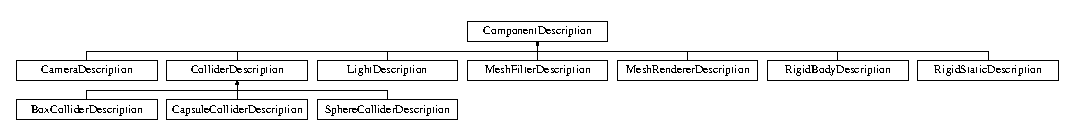
\includegraphics[height=1.379310cm]{class_component_description}
\end{center}
\end{figure}
\subsection*{Public Attributes}
\begin{DoxyCompactItemize}
\item 
\hypertarget{class_component_description_a44f422a98827af2805af6f58124aa23f}{}Component\+Type {\bfseries type}\label{class_component_description_a44f422a98827af2805af6f58124aa23f}

\end{DoxyCompactItemize}


The documentation for this class was generated from the following file\+:\begin{DoxyCompactItemize}
\item 
/\+Users/guilherme\+\_\+cunha/\+Dev/\+G\+I\+T\+H\+U\+B/\+G\+U\+Inity/\+Source/Serialization\+Structs.\+hpp\end{DoxyCompactItemize}

\hypertarget{classconcrete__type}{}\section{concrete\+\_\+type$<$ T $>$ Class Template Reference}
\label{classconcrete__type}\index{concrete\+\_\+type$<$ T $>$@{concrete\+\_\+type$<$ T $>$}}
Inheritance diagram for concrete\+\_\+type$<$ T $>$\+:\begin{figure}[H]
\begin{center}
\leavevmode
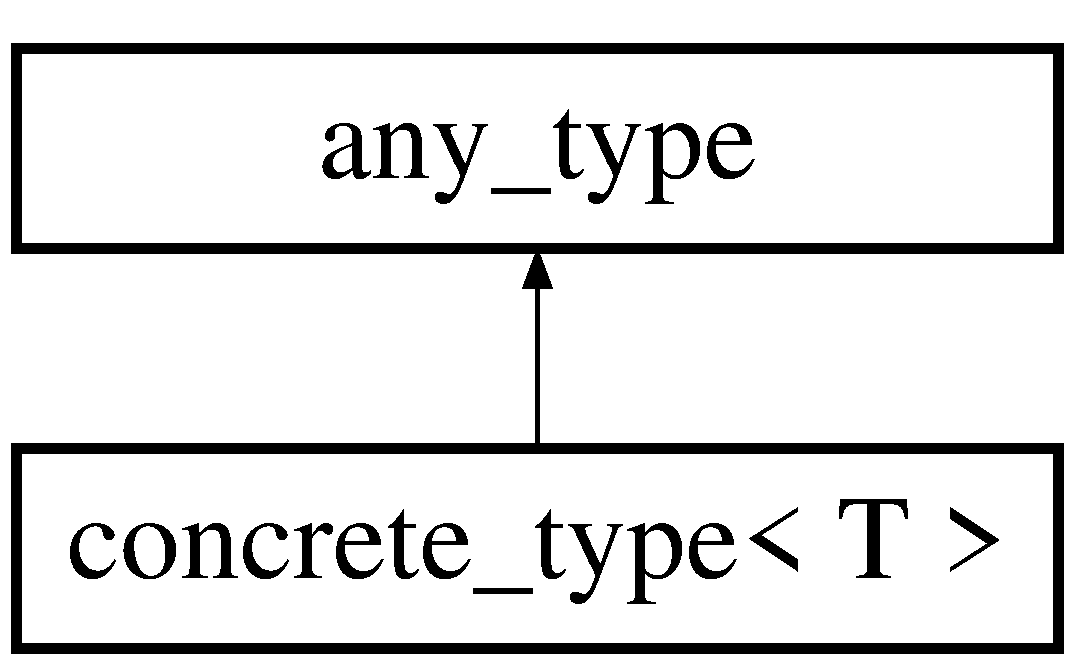
\includegraphics[height=2.000000cm]{classconcrete__type}
\end{center}
\end{figure}
\subsection*{Public Member Functions}
\begin{DoxyCompactItemize}
\item 
\hypertarget{classconcrete__type_ad0e185e3b1a29e1cb3e25c3db6993846}{}{\bfseries concrete\+\_\+type} (const T \&value)\label{classconcrete__type_ad0e185e3b1a29e1cb3e25c3db6993846}

\item 
\hypertarget{classconcrete__type_aa7da74fe0fea3d295f555ac3df96b937}{}virtual void {\bfseries print} ()\label{classconcrete__type_aa7da74fe0fea3d295f555ac3df96b937}

\end{DoxyCompactItemize}


The documentation for this class was generated from the following file\+:\begin{DoxyCompactItemize}
\item 
/\+Users/guilherme\+\_\+cunha/\+Dev/\+G\+I\+T\+H\+U\+B/\+G\+U\+Inity/\+Source/Any\+Class.\+hpp\end{DoxyCompactItemize}

\hypertarget{class_editor}{}\section{Editor Class Reference}
\label{class_editor}\index{Editor@{Editor}}
Inheritance diagram for Editor\+:\begin{figure}[H]
\begin{center}
\leavevmode
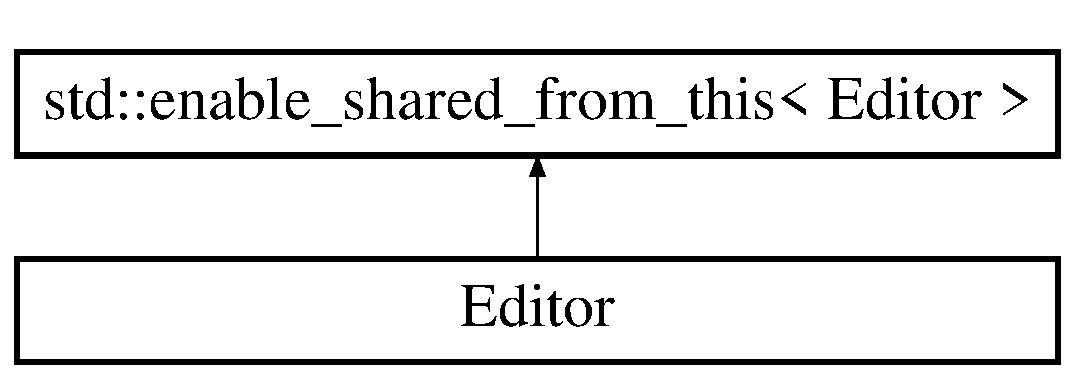
\includegraphics[height=2.000000cm]{class_editor}
\end{center}
\end{figure}
\subsection*{Static Public Member Functions}
\begin{DoxyCompactItemize}
\item 
\hypertarget{class_editor_a7cb836a93ceab82c32f159dcfe2b21e4}{}static void {\bfseries init} ()\label{class_editor_a7cb836a93ceab82c32f159dcfe2b21e4}

\item 
\hypertarget{class_editor_a5c88c86f921600ca0d2fc28fcc12bf95}{}static void {\bfseries shutdown} ()\label{class_editor_a5c88c86f921600ca0d2fc28fcc12bf95}

\item 
\hypertarget{class_editor_a4b2a1fd5918cd45445c727db802d9067}{}static void {\bfseries update} (float delta\+Seconds, shared\+\_\+ptr$<$ \hyperlink{class_world}{World} $>$ game\+World)\label{class_editor_a4b2a1fd5918cd45445c727db802d9067}

\end{DoxyCompactItemize}
\subsection*{Static Public Attributes}
\begin{DoxyCompactItemize}
\item 
\hypertarget{class_editor_a9987cc7ae7fb52189734079b80eab220}{}static shared\+\_\+ptr$<$ \hyperlink{class_actor}{Actor} $>$ {\bfseries camera\+Actor}\label{class_editor_a9987cc7ae7fb52189734079b80eab220}

\item 
\hypertarget{class_editor_a7b66261f82c8365732054171784725cc}{}static shared\+\_\+ptr$<$ \hyperlink{class_camera}{Camera} $>$ {\bfseries camera\+Component}\label{class_editor_a7b66261f82c8365732054171784725cc}

\item 
\hypertarget{class_editor_af478b09e584532e9de994255394a7ba6}{}static shared\+\_\+ptr$<$ \hyperlink{class_world}{World} $>$ {\bfseries world}\label{class_editor_af478b09e584532e9de994255394a7ba6}

\item 
\hypertarget{class_editor_a11095b5f6f42d73b6572e59225d616ed}{}static shared\+\_\+ptr$<$ \hyperlink{class_actor}{Actor} $>$ {\bfseries current\+Selected\+Actor}\label{class_editor_a11095b5f6f42d73b6572e59225d616ed}

\item 
\hypertarget{class_editor_a2bb668ff0442c826055eea8996afec0e}{}static shared\+\_\+ptr$<$ \hyperlink{class_actor}{Actor} $>$ {\bfseries move\+Handles}\label{class_editor_a2bb668ff0442c826055eea8996afec0e}

\item 
\hypertarget{class_editor_a08dcbe3de2ae85741f28748ed92335e5}{}static shared\+\_\+ptr$<$ \hyperlink{class_actor}{Actor} $>$ {\bfseries rotate\+Handles}\label{class_editor_a08dcbe3de2ae85741f28748ed92335e5}

\item 
\hypertarget{class_editor_a6ae097c81fc7631122e2be5a5c3d7ae5}{}static shared\+\_\+ptr$<$ \hyperlink{class_actor}{Actor} $>$ {\bfseries scale\+Handles}\label{class_editor_a6ae097c81fc7631122e2be5a5c3d7ae5}

\item 
\hypertarget{class_editor_a9169638c34360328cbbb6f731bb1b3ea}{}static shared\+\_\+ptr$<$ U\+I\+Widget $>$ {\bfseries ui\+Widget\+Test}\label{class_editor_a9169638c34360328cbbb6f731bb1b3ea}

\item 
\hypertarget{class_editor_a5d3ea528bdefe9cd342bccc6a6ab3af3}{}static Transform\+Mode {\bfseries transform\+Mode}\label{class_editor_a5d3ea528bdefe9cd342bccc6a6ab3af3}

\end{DoxyCompactItemize}


The documentation for this class was generated from the following files\+:\begin{DoxyCompactItemize}
\item 
/\+Users/guilherme\+\_\+cunha/\+Dev/\+G\+I\+T\+H\+U\+B/\+G\+U\+Inity/\+Source/Editor.\+hpp\item 
/\+Users/guilherme\+\_\+cunha/\+Dev/\+G\+I\+T\+H\+U\+B/\+G\+U\+Inity/\+Source/Editor.\+cpp\end{DoxyCompactItemize}

\hypertarget{class_editor_camera_control}{}\section{Editor\+Camera\+Control Class Reference}
\label{class_editor_camera_control}\index{Editor\+Camera\+Control@{Editor\+Camera\+Control}}
Inheritance diagram for Editor\+Camera\+Control\+:\begin{figure}[H]
\begin{center}
\leavevmode
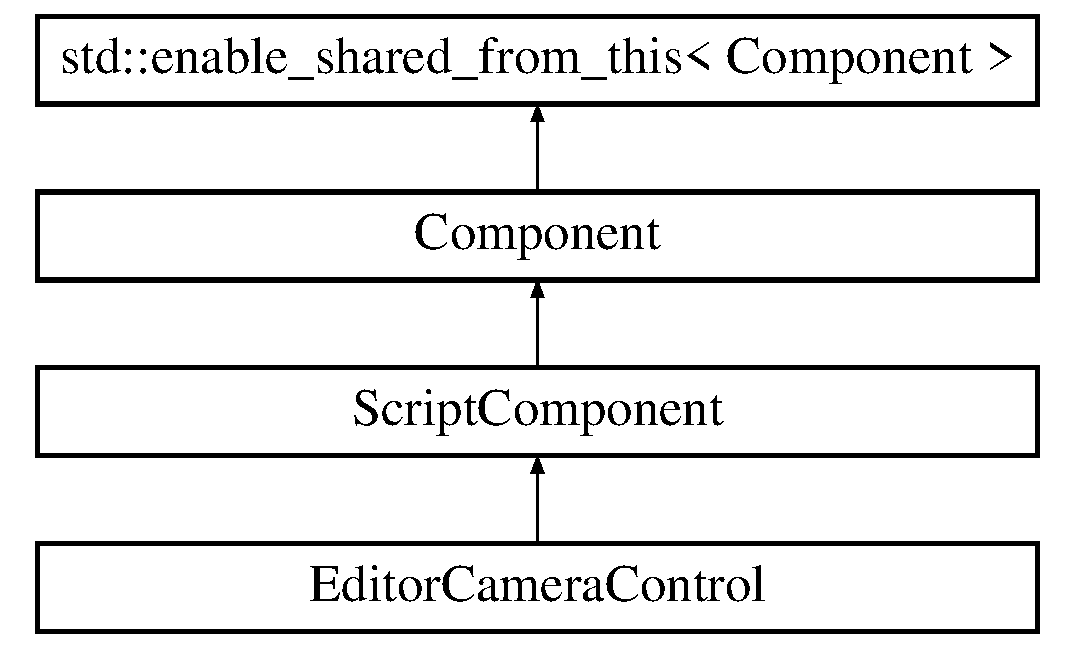
\includegraphics[height=4.000000cm]{class_editor_camera_control}
\end{center}
\end{figure}
\subsection*{Public Member Functions}
\begin{DoxyCompactItemize}
\item 
virtual void \hyperlink{class_editor_camera_control_af672d52ea342e6762f9f104898959181}{init} ()
\item 
virtual void \hyperlink{class_editor_camera_control_a829966c94f5f99911a20534692dcc78f}{tick} (float delta\+Seconds)
\end{DoxyCompactItemize}
\subsection*{Public Attributes}
\begin{DoxyCompactItemize}
\item 
\hypertarget{class_editor_camera_control_a5297aa27db37eabd8ba5c6927e7635ab}{}float {\bfseries move\+Speed}\label{class_editor_camera_control_a5297aa27db37eabd8ba5c6927e7635ab}

\item 
\hypertarget{class_editor_camera_control_a2c9b2cd83d46061b6f7f2afc26e708b3}{}float {\bfseries rotation\+Speed}\label{class_editor_camera_control_a2c9b2cd83d46061b6f7f2afc26e708b3}

\end{DoxyCompactItemize}
\subsection*{Additional Inherited Members}


\subsection{Member Function Documentation}
\hypertarget{class_editor_camera_control_af672d52ea342e6762f9f104898959181}{}\index{Editor\+Camera\+Control@{Editor\+Camera\+Control}!init@{init}}
\index{init@{init}!Editor\+Camera\+Control@{Editor\+Camera\+Control}}
\subsubsection[{init()}]{\setlength{\rightskip}{0pt plus 5cm}void Editor\+Camera\+Control\+::init (
\begin{DoxyParamCaption}
{}
\end{DoxyParamCaption}
)\hspace{0.3cm}{\ttfamily [virtual]}}\label{class_editor_camera_control_af672d52ea342e6762f9f104898959181}
\hyperlink{class_component}{Component} init override 

Reimplemented from \hyperlink{class_script_component_a6fb8a859ed628b7b97801a2b3fb4f8ea}{Script\+Component}.

\hypertarget{class_editor_camera_control_a829966c94f5f99911a20534692dcc78f}{}\index{Editor\+Camera\+Control@{Editor\+Camera\+Control}!tick@{tick}}
\index{tick@{tick}!Editor\+Camera\+Control@{Editor\+Camera\+Control}}
\subsubsection[{tick(float delta\+Seconds)}]{\setlength{\rightskip}{0pt plus 5cm}void Editor\+Camera\+Control\+::tick (
\begin{DoxyParamCaption}
\item[{float}]{delta\+Secods}
\end{DoxyParamCaption}
)\hspace{0.3cm}{\ttfamily [virtual]}}\label{class_editor_camera_control_a829966c94f5f99911a20534692dcc78f}
\hyperlink{class_component}{Component} tick override 
\begin{DoxyParams}[1]{Parameters}
\mbox{\tt in}  & {\em delta\+Seconds} & last frame durations \\
\hline
\end{DoxyParams}


Reimplemented from \hyperlink{class_script_component_aa765fa62a343a8d83eb168d369b93a51}{Script\+Component}.



The documentation for this class was generated from the following files\+:\begin{DoxyCompactItemize}
\item 
/\+Users/guilherme\+\_\+cunha/\+Dev/\+G\+I\+T\+H\+U\+B/\+G\+U\+Inity/\+Source/Editor\+Camera\+Control.\+hpp\item 
/\+Users/guilherme\+\_\+cunha/\+Dev/\+G\+I\+T\+H\+U\+B/\+G\+U\+Inity/\+Source/Editor\+Camera\+Control.\+cpp\end{DoxyCompactItemize}

\hypertarget{class_editor_collider}{}\section{Editor\+Collider Class Reference}
\label{class_editor_collider}\index{Editor\+Collider@{Editor\+Collider}}


{\ttfamily \#include $<$Editor\+Collider.\+hpp$>$}

Inheritance diagram for Editor\+Collider\+:\begin{figure}[H]
\begin{center}
\leavevmode
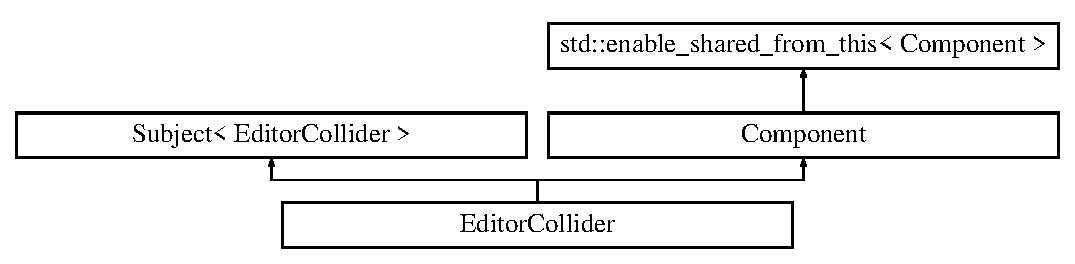
\includegraphics[height=3.000000cm]{class_editor_collider}
\end{center}
\end{figure}
\subsection*{Public Member Functions}
\begin{DoxyCompactItemize}
\item 
\hyperlink{class_editor_collider_a2f042fd2b14c9e45aa7227568d795424}{Editor\+Collider} ()
\item 
virtual \hyperlink{class_editor_collider_a2dbee537bb0ce1f9b57d78b1c60431d5}{$\sim$\+Editor\+Collider} ()
\item 
virtual void \hyperlink{class_editor_collider_a6581dd66dd2881b0faafe6975b4a188c}{init} () override
\item 
virtual void \hyperlink{class_editor_collider_a0ffb1252a656a1ec84d3492052bf3cee}{tick} (float delta\+Seconds) override
\item 
void \hyperlink{class_editor_collider_ad93e80e2f9faf19633976f1694740bc2}{set\+Game\+Actor} (shared\+\_\+ptr$<$ \hyperlink{class_actor}{Actor} $>$ game\+Actor)
\item 
shared\+\_\+ptr$<$ \hyperlink{class_actor}{Actor} $>$ \hyperlink{class_editor_collider_ac2feb06d18c27ca29f06d5a70e48f9a1}{get\+Game\+Actor} ()
\item 
Px\+Rigid\+Dynamic $\ast$ \hyperlink{class_editor_collider_a0f422a9ae779f98053e18a1bec4a200a}{get\+Rigid\+Static} ()
\item 
virtual shared\+\_\+ptr$<$ \hyperlink{class_component}{Component} $>$ \hyperlink{class_editor_collider_abfee383f62b5bc06afffe5beedb729e3}{clone} () override
\item 
virtual shared\+\_\+ptr$<$ \hyperlink{class_component_description}{Component\+Description} $>$ \hyperlink{group__serialization__functions_gac3df1d451d142f9ec123c0439cd503eb}{get\+Component\+Description} () override
\item 
virtual void \hyperlink{group__serialization__functions_ga9b02f2f116742850f196d8fc84e50af8}{deserialize} (shared\+\_\+ptr$<$ \hyperlink{class_component_description}{Component\+Description} $>$ desc) override
\end{DoxyCompactItemize}
\subsection*{Additional Inherited Members}


\subsection{Detailed Description}
\hyperlink{class_editor_collider}{Editor\+Collider} is a component used only by editor actors. They\textquotesingle{}re used for queries only, so that when the user clicks on whatever \hyperlink{class_actor}{Actor} in the scene, we can find it using Phys\+X queries. The basic difference between the \hyperlink{class_editor_collider}{Editor\+Collider} and the regular \hyperlink{class_collider}{Collider} is that this one has a reference to the real \hyperlink{class_game}{Game} \hyperlink{class_actor}{Actor}. 

\subsection{Constructor \& Destructor Documentation}
\hypertarget{class_editor_collider_a2f042fd2b14c9e45aa7227568d795424}{}\index{Editor\+Collider@{Editor\+Collider}!Editor\+Collider@{Editor\+Collider}}
\index{Editor\+Collider@{Editor\+Collider}!Editor\+Collider@{Editor\+Collider}}
\subsubsection[{Editor\+Collider()}]{\setlength{\rightskip}{0pt plus 5cm}Editor\+Collider\+::\+Editor\+Collider (
\begin{DoxyParamCaption}
{}
\end{DoxyParamCaption}
)\hspace{0.3cm}{\ttfamily [inline]}}\label{class_editor_collider_a2f042fd2b14c9e45aa7227568d795424}
Default Constructor \hypertarget{class_editor_collider_a2dbee537bb0ce1f9b57d78b1c60431d5}{}\index{Editor\+Collider@{Editor\+Collider}!````~Editor\+Collider@{$\sim$\+Editor\+Collider}}
\index{````~Editor\+Collider@{$\sim$\+Editor\+Collider}!Editor\+Collider@{Editor\+Collider}}
\subsubsection[{$\sim$\+Editor\+Collider()}]{\setlength{\rightskip}{0pt plus 5cm}virtual Editor\+Collider\+::$\sim$\+Editor\+Collider (
\begin{DoxyParamCaption}
{}
\end{DoxyParamCaption}
)\hspace{0.3cm}{\ttfamily [inline]}, {\ttfamily [virtual]}}\label{class_editor_collider_a2dbee537bb0ce1f9b57d78b1c60431d5}
Default Destructor. Virtual because inherits from \hyperlink{class_component}{Component} 

\subsection{Member Function Documentation}
\hypertarget{class_editor_collider_abfee383f62b5bc06afffe5beedb729e3}{}\index{Editor\+Collider@{Editor\+Collider}!clone@{clone}}
\index{clone@{clone}!Editor\+Collider@{Editor\+Collider}}
\subsubsection[{clone() override}]{\setlength{\rightskip}{0pt plus 5cm}shared\+\_\+ptr$<$ {\bf Component} $>$ Editor\+Collider\+::clone (
\begin{DoxyParamCaption}
{}
\end{DoxyParamCaption}
)\hspace{0.3cm}{\ttfamily [override]}, {\ttfamily [virtual]}}\label{class_editor_collider_abfee383f62b5bc06afffe5beedb729e3}
Clones current component (Prototype Design Pattern) \begin{DoxyReturn}{Returns}
nullptr, Editor\+Colliders are not supposed to be cloned 
\end{DoxyReturn}


Implements \hyperlink{class_component_a74c984bd819bbef16fd4f306a90d34fe}{Component}.

\hypertarget{class_editor_collider_ac2feb06d18c27ca29f06d5a70e48f9a1}{}\index{Editor\+Collider@{Editor\+Collider}!get\+Game\+Actor@{get\+Game\+Actor}}
\index{get\+Game\+Actor@{get\+Game\+Actor}!Editor\+Collider@{Editor\+Collider}}
\subsubsection[{get\+Game\+Actor()}]{\setlength{\rightskip}{0pt plus 5cm}shared\+\_\+ptr$<$ {\bf Actor} $>$ Editor\+Collider\+::get\+Game\+Actor (
\begin{DoxyParamCaption}
{}
\end{DoxyParamCaption}
)}\label{class_editor_collider_ac2feb06d18c27ca29f06d5a70e48f9a1}
game\+Actor getter \hypertarget{class_editor_collider_a0f422a9ae779f98053e18a1bec4a200a}{}\index{Editor\+Collider@{Editor\+Collider}!get\+Rigid\+Static@{get\+Rigid\+Static}}
\index{get\+Rigid\+Static@{get\+Rigid\+Static}!Editor\+Collider@{Editor\+Collider}}
\subsubsection[{get\+Rigid\+Static()}]{\setlength{\rightskip}{0pt plus 5cm}Px\+Rigid\+Dynamic $\ast$ Editor\+Collider\+::get\+Rigid\+Static (
\begin{DoxyParamCaption}
{}
\end{DoxyParamCaption}
)}\label{class_editor_collider_a0f422a9ae779f98053e18a1bec4a200a}
physx\+Rigid\+Static getter \hypertarget{class_editor_collider_a6581dd66dd2881b0faafe6975b4a188c}{}\index{Editor\+Collider@{Editor\+Collider}!init@{init}}
\index{init@{init}!Editor\+Collider@{Editor\+Collider}}
\subsubsection[{init() override}]{\setlength{\rightskip}{0pt plus 5cm}void Editor\+Collider\+::init (
\begin{DoxyParamCaption}
{}
\end{DoxyParamCaption}
)\hspace{0.3cm}{\ttfamily [override]}, {\ttfamily [virtual]}}\label{class_editor_collider_a6581dd66dd2881b0faafe6975b4a188c}
\hyperlink{class_component}{Component} init override. Initializes the rigid body in the Phys\+X scene.

\hyperlink{class_component}{Component} tick override. Updates the fake collider position and rotation to match the real \hyperlink{class_game}{Game} \hyperlink{class_actor}{Actor} 

Reimplemented from \hyperlink{class_component_a162f8cdc070537a71f2ad0b5e763b86f}{Component}.

\hypertarget{class_editor_collider_ad93e80e2f9faf19633976f1694740bc2}{}\index{Editor\+Collider@{Editor\+Collider}!set\+Game\+Actor@{set\+Game\+Actor}}
\index{set\+Game\+Actor@{set\+Game\+Actor}!Editor\+Collider@{Editor\+Collider}}
\subsubsection[{set\+Game\+Actor(shared\+\_\+ptr$<$ Actor $>$ game\+Actor)}]{\setlength{\rightskip}{0pt plus 5cm}void Editor\+Collider\+::set\+Game\+Actor (
\begin{DoxyParamCaption}
\item[{shared\+\_\+ptr$<$ {\bf Actor} $>$}]{game\+Actor}
\end{DoxyParamCaption}
)}\label{class_editor_collider_ad93e80e2f9faf19633976f1694740bc2}
game\+Actor setter \hypertarget{class_editor_collider_a0ffb1252a656a1ec84d3492052bf3cee}{}\index{Editor\+Collider@{Editor\+Collider}!tick@{tick}}
\index{tick@{tick}!Editor\+Collider@{Editor\+Collider}}
\subsubsection[{tick(float delta\+Seconds) override}]{\setlength{\rightskip}{0pt plus 5cm}void Editor\+Collider\+::tick (
\begin{DoxyParamCaption}
\item[{float}]{delta\+Seconds}
\end{DoxyParamCaption}
)\hspace{0.3cm}{\ttfamily [override]}, {\ttfamily [virtual]}}\label{class_editor_collider_a0ffb1252a656a1ec84d3492052bf3cee}
\hyperlink{class_component}{Component} tick override. Updates the fake collider position and rotation to match the real \hyperlink{class_game}{Game} \hyperlink{class_actor}{Actor}

\hyperlink{class_component}{Component} init override. Initializes the rigid body in the Phys\+X scene. 

Reimplemented from \hyperlink{class_component_a72d67b02e6733c1a6fb73cbaaf8ebff4}{Component}.



The documentation for this class was generated from the following files\+:\begin{DoxyCompactItemize}
\item 
/\+Users/guilherme\+\_\+cunha/\+Dev/\+G\+I\+T\+H\+U\+B/\+G\+U\+Inity/\+Source/Editor\+Collider.\+hpp\item 
/\+Users/guilherme\+\_\+cunha/\+Dev/\+G\+I\+T\+H\+U\+B/\+G\+U\+Inity/\+Source/Editor\+Collider.\+cpp\end{DoxyCompactItemize}

\hypertarget{class_factory}{}\section{Factory Class Reference}
\label{class_factory}\index{Factory@{Factory}}


{\ttfamily \#include $<$Factory.\+hpp$>$}

Inheritance diagram for Factory\+:\begin{figure}[H]
\begin{center}
\leavevmode
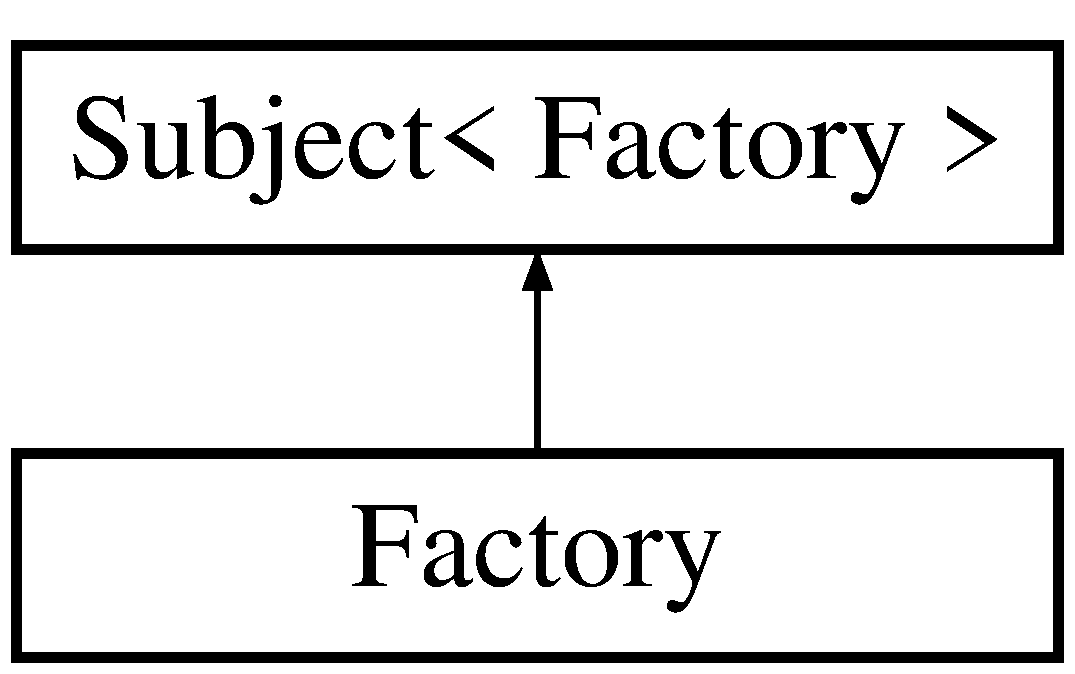
\includegraphics[height=2.000000cm]{class_factory}
\end{center}
\end{figure}
\subsection*{Public Member Functions}
\begin{DoxyCompactItemize}
\item 
\hyperlink{class_factory_ac792bf88cfb7b6804b479529da5308cc}{Factory} ()
\item 
\hyperlink{class_factory_a8f71456f48e4df402c778a44191ff40e}{$\sim$\+Factory} ()
\end{DoxyCompactItemize}
\subsection*{Static Public Member Functions}
\begin{DoxyCompactItemize}
\item 
static shared\+\_\+ptr$<$ \hyperlink{class_actor}{Actor} $>$ \hyperlink{class_factory_a4d1f778e641569328fda27d6faf7b795}{Create\+Actor} (string name)
\item 
static void \hyperlink{class_factory_ac6f0a190052296cc9986fb6b5c7e0d60}{Destroy\+Actor} (weak\+\_\+ptr$<$ \hyperlink{class_actor}{Actor} $>$ actor)
\item 
static void \hyperlink{class_factory_a8ff3b9e48200289837a92865aae6c6aa}{Create\+Reference\+Actor} (shared\+\_\+ptr$<$ \hyperlink{class_actor}{Actor} $>$ real\+Actor)
\item 
static shared\+\_\+ptr$<$ \hyperlink{class_actor}{Actor} $>$ \hyperlink{class_factory_a793822c87c9d0c0c8519527ea5b294a9}{Create\+Editor\+Actor} (string name)
\item 
static void \hyperlink{class_factory_a7f56d55416496af6a2c75c62277d4f9c}{Deserialize\+Components} (shared\+\_\+ptr$<$ \hyperlink{class_actor}{Actor} $>$ actor, vector$<$ shared\+\_\+ptr$<$ \hyperlink{class_component_description}{Component\+Description} $>$$>$ comp\+Descs)
\item 
static shared\+\_\+ptr$<$ \hyperlink{class_actor}{Actor} $>$ \hyperlink{class_factory_a017c0ac2bad4a9517443e8ef51601d1c}{Deserialize\+Actor} (\hyperlink{struct_actor_description}{Actor\+Description} \&desc)
\end{DoxyCompactItemize}
\subsection*{Additional Inherited Members}


\subsection{Detailed Description}
\hyperlink{class_actor}{Actor} \hyperlink{class_factory}{Factory}

This class is responsible for creating new actors. Actors should not be created by hand, but using the \hyperlink{class_factory}{Factory} instead. This class also holds the model of each \hyperlink{class_component}{Component} for the Prototype Design Pattern. 

\subsection{Constructor \& Destructor Documentation}
\hypertarget{class_factory_ac792bf88cfb7b6804b479529da5308cc}{}\index{Factory@{Factory}!Factory@{Factory}}
\index{Factory@{Factory}!Factory@{Factory}}
\subsubsection[{Factory()}]{\setlength{\rightskip}{0pt plus 5cm}Factory\+::\+Factory (
\begin{DoxyParamCaption}
{}
\end{DoxyParamCaption}
)\hspace{0.3cm}{\ttfamily [inline]}}\label{class_factory_ac792bf88cfb7b6804b479529da5308cc}
Default Constructor \hypertarget{class_factory_a8f71456f48e4df402c778a44191ff40e}{}\index{Factory@{Factory}!````~Factory@{$\sim$\+Factory}}
\index{````~Factory@{$\sim$\+Factory}!Factory@{Factory}}
\subsubsection[{$\sim$\+Factory()}]{\setlength{\rightskip}{0pt plus 5cm}Factory\+::$\sim$\+Factory (
\begin{DoxyParamCaption}
{}
\end{DoxyParamCaption}
)\hspace{0.3cm}{\ttfamily [inline]}}\label{class_factory_a8f71456f48e4df402c778a44191ff40e}
Default Destructory 

\subsection{Member Function Documentation}
\hypertarget{class_factory_a4d1f778e641569328fda27d6faf7b795}{}\index{Factory@{Factory}!Create\+Actor@{Create\+Actor}}
\index{Create\+Actor@{Create\+Actor}!Factory@{Factory}}
\subsubsection[{Create\+Actor(string name)}]{\setlength{\rightskip}{0pt plus 5cm}shared\+\_\+ptr$<$ {\bf Actor} $>$ Factory\+::\+Create\+Actor (
\begin{DoxyParamCaption}
\item[{string}]{name}
\end{DoxyParamCaption}
)\hspace{0.3cm}{\ttfamily [static]}}\label{class_factory_a4d1f778e641569328fda27d6faf7b795}
Create a new \hyperlink{class_actor}{Actor} \hypertarget{class_factory_a793822c87c9d0c0c8519527ea5b294a9}{}\index{Factory@{Factory}!Create\+Editor\+Actor@{Create\+Editor\+Actor}}
\index{Create\+Editor\+Actor@{Create\+Editor\+Actor}!Factory@{Factory}}
\subsubsection[{Create\+Editor\+Actor(string name)}]{\setlength{\rightskip}{0pt plus 5cm}shared\+\_\+ptr$<$ {\bf Actor} $>$ Factory\+::\+Create\+Editor\+Actor (
\begin{DoxyParamCaption}
\item[{string}]{name}
\end{DoxyParamCaption}
)\hspace{0.3cm}{\ttfamily [static]}}\label{class_factory_a793822c87c9d0c0c8519527ea5b294a9}
Create a new \hyperlink{class_editor}{Editor} \hyperlink{class_actor}{Actor}, one that lives only in the \hyperlink{class_editor}{Editor} \hyperlink{class_world}{World} \hypertarget{class_factory_a8ff3b9e48200289837a92865aae6c6aa}{}\index{Factory@{Factory}!Create\+Reference\+Actor@{Create\+Reference\+Actor}}
\index{Create\+Reference\+Actor@{Create\+Reference\+Actor}!Factory@{Factory}}
\subsubsection[{Create\+Reference\+Actor(shared\+\_\+ptr$<$ Actor $>$ real\+Actor)}]{\setlength{\rightskip}{0pt plus 5cm}void Factory\+::\+Create\+Reference\+Actor (
\begin{DoxyParamCaption}
\item[{shared\+\_\+ptr$<$ {\bf Actor} $>$}]{real\+Actor}
\end{DoxyParamCaption}
)\hspace{0.3cm}{\ttfamily [static]}}\label{class_factory_a8ff3b9e48200289837a92865aae6c6aa}
Create reference actor. Every \hyperlink{class_actor}{Actor} in the \hyperlink{class_game}{Game} \hyperlink{class_world}{World} has a Reference \hyperlink{class_actor}{Actor} in the \hyperlink{class_editor}{Editor} \hyperlink{class_world}{World} to allow them to be manipulated \hypertarget{class_factory_a017c0ac2bad4a9517443e8ef51601d1c}{}\index{Factory@{Factory}!Deserialize\+Actor@{Deserialize\+Actor}}
\index{Deserialize\+Actor@{Deserialize\+Actor}!Factory@{Factory}}
\subsubsection[{Deserialize\+Actor(\+Actor\+Description \&desc)}]{\setlength{\rightskip}{0pt plus 5cm}shared\+\_\+ptr$<$ {\bf Actor} $>$ Factory\+::\+Deserialize\+Actor (
\begin{DoxyParamCaption}
\item[{{\bf Actor\+Description} \&}]{desc}
\end{DoxyParamCaption}
)\hspace{0.3cm}{\ttfamily [static]}}\label{class_factory_a017c0ac2bad4a9517443e8ef51601d1c}
Deserialize an \hyperlink{class_actor}{Actor} \hypertarget{class_factory_a7f56d55416496af6a2c75c62277d4f9c}{}\index{Factory@{Factory}!Deserialize\+Components@{Deserialize\+Components}}
\index{Deserialize\+Components@{Deserialize\+Components}!Factory@{Factory}}
\subsubsection[{Deserialize\+Components(shared\+\_\+ptr$<$ Actor $>$ actor, vector$<$ shared\+\_\+ptr$<$ Component\+Description $>$$>$ comp\+Descs)}]{\setlength{\rightskip}{0pt plus 5cm}void Factory\+::\+Deserialize\+Components (
\begin{DoxyParamCaption}
\item[{shared\+\_\+ptr$<$ {\bf Actor} $>$}]{actor, }
\item[{vector$<$ shared\+\_\+ptr$<$ {\bf Component\+Description} $>$$>$}]{comp\+Descs}
\end{DoxyParamCaption}
)\hspace{0.3cm}{\ttfamily [static]}}\label{class_factory_a7f56d55416496af6a2c75c62277d4f9c}
Deserialize a list of Components and attaches them to an \hyperlink{class_actor}{Actor} \hypertarget{class_factory_ac6f0a190052296cc9986fb6b5c7e0d60}{}\index{Factory@{Factory}!Destroy\+Actor@{Destroy\+Actor}}
\index{Destroy\+Actor@{Destroy\+Actor}!Factory@{Factory}}
\subsubsection[{Destroy\+Actor(weak\+\_\+ptr$<$ Actor $>$ actor)}]{\setlength{\rightskip}{0pt plus 5cm}void Factory\+::\+Destroy\+Actor (
\begin{DoxyParamCaption}
\item[{weak\+\_\+ptr$<$ {\bf Actor} $>$}]{actor}
\end{DoxyParamCaption}
)\hspace{0.3cm}{\ttfamily [static]}}\label{class_factory_ac6f0a190052296cc9986fb6b5c7e0d60}
Destroys an \hyperlink{class_actor}{Actor}

Create a new \hyperlink{class_actor}{Actor} 

The documentation for this class was generated from the following files\+:\begin{DoxyCompactItemize}
\item 
/\+Users/guilherme\+\_\+cunha/\+Dev/\+G\+I\+T\+H\+U\+B/\+G\+U\+Inity/\+Source/Factory.\+hpp\item 
/\+Users/guilherme\+\_\+cunha/\+Dev/\+G\+I\+T\+H\+U\+B/\+G\+U\+Inity/\+Source/Factory.\+cpp\end{DoxyCompactItemize}

\hypertarget{class_font}{}\section{Font Class Reference}
\label{class_font}\index{Font@{Font}}


{\ttfamily \#include $<$Font.\+hpp$>$}

Inheritance diagram for Font\+:\begin{figure}[H]
\begin{center}
\leavevmode
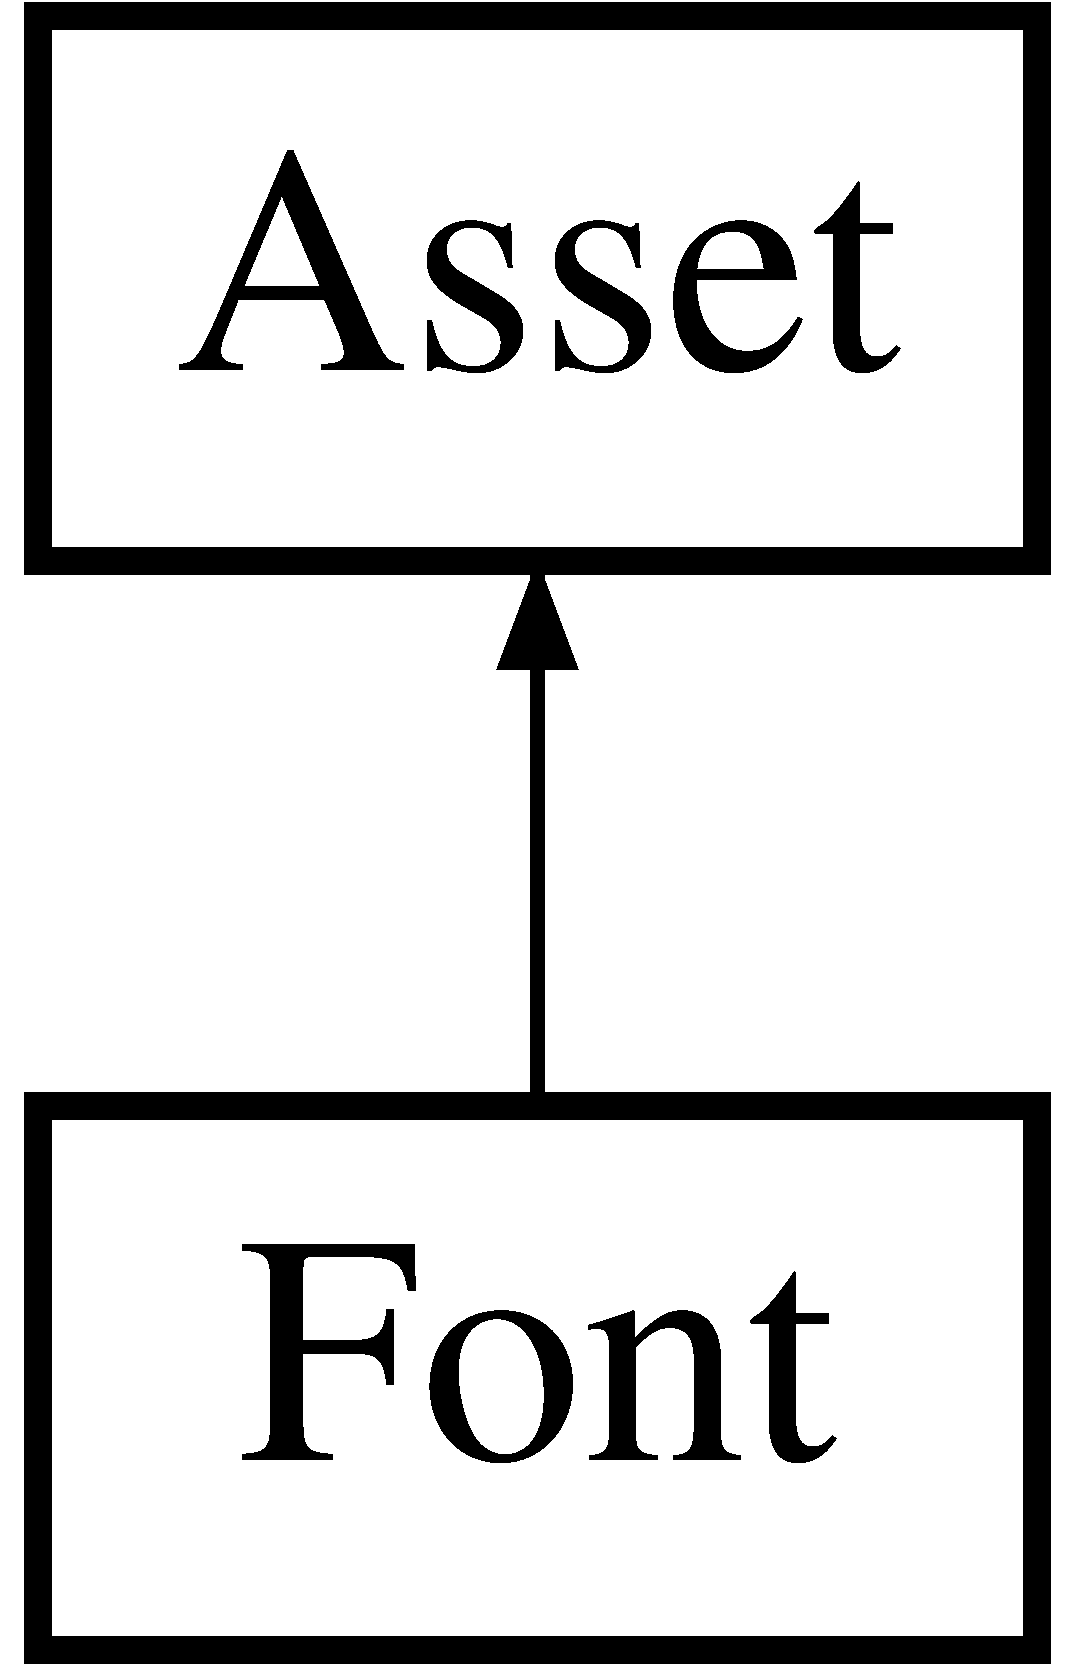
\includegraphics[height=2.000000cm]{class_font}
\end{center}
\end{figure}
\subsection*{Public Member Functions}
\begin{DoxyCompactItemize}
\item 
\hyperlink{class_font_ab17ce6ae9fe536a4b8cf3ecf2b8d4913}{Font} (shared\+\_\+ptr$<$ \hyperlink{class_texture}{Texture} $>$ font\+Texture, map$<$ char, \hyperlink{struct_letter_font_u_v}{Letter\+Font\+U\+V} $>$ char\+U\+V\+Map, int font\+Size)
\item 
virtual \hyperlink{class_font_afcb2c2e708187a600a6129e2719bcd81}{$\sim$\+Font} ()
\item 
shared\+\_\+ptr$<$ \hyperlink{class_texture}{Texture} $>$ \hyperlink{class_font_a4aeb5630943d4b9d65030c108291c874}{get\+Font\+Texture} ()
\item 
int \hyperlink{class_font_a3f4d697a2464f49dcdb92e7735e096a2}{get\+Font\+Size} ()
\item 
map$<$ char, \hyperlink{struct_letter_font_u_v}{Letter\+Font\+U\+V} $>$ \hyperlink{class_font_a880e278802c289b129600856d297d8ff}{get\+Char\+U\+V\+Map} ()
\item 
\hyperlink{struct_letter_font_u_v}{Letter\+Font\+U\+V} \hyperlink{class_font_a9a3127bceaad861d759a2f52e9b479e4}{get\+Char\+Desc} (char c)
\end{DoxyCompactItemize}


\subsection{Detailed Description}
\hyperlink{class_font}{Font} is an \hyperlink{class_asset}{Asset}. It holds the information of the font size, the available characters and their U\+V mapping to the corresponding \hyperlink{class_texture}{Texture} 

\subsection{Constructor \& Destructor Documentation}
\hypertarget{class_font_ab17ce6ae9fe536a4b8cf3ecf2b8d4913}{}\index{Font@{Font}!Font@{Font}}
\index{Font@{Font}!Font@{Font}}
\subsubsection[{Font(shared\+\_\+ptr$<$ Texture $>$ font\+Texture, map$<$ char, Letter\+Font\+U\+V $>$ char\+U\+V\+Map, int font\+Size)}]{\setlength{\rightskip}{0pt plus 5cm}Font\+::\+Font (
\begin{DoxyParamCaption}
\item[{shared\+\_\+ptr$<$ {\bf Texture} $>$}]{font\+Texture, }
\item[{map$<$ char, {\bf Letter\+Font\+U\+V} $>$}]{char\+U\+V\+Map, }
\item[{int}]{font\+Size}
\end{DoxyParamCaption}
)}\label{class_font_ab17ce6ae9fe536a4b8cf3ecf2b8d4913}
Constructor from a \hyperlink{class_texture}{Texture}, a map of available chars and their U\+V\+Mapping and the font size. \hypertarget{class_font_afcb2c2e708187a600a6129e2719bcd81}{}\index{Font@{Font}!````~Font@{$\sim$\+Font}}
\index{````~Font@{$\sim$\+Font}!Font@{Font}}
\subsubsection[{$\sim$\+Font()}]{\setlength{\rightskip}{0pt plus 5cm}virtual Font\+::$\sim$\+Font (
\begin{DoxyParamCaption}
{}
\end{DoxyParamCaption}
)\hspace{0.3cm}{\ttfamily [inline]}, {\ttfamily [virtual]}}\label{class_font_afcb2c2e708187a600a6129e2719bcd81}
Default Destructor. Virtual cause it\textquotesingle{}s children class 

\subsection{Member Function Documentation}
\hypertarget{class_font_a9a3127bceaad861d759a2f52e9b479e4}{}\index{Font@{Font}!get\+Char\+Desc@{get\+Char\+Desc}}
\index{get\+Char\+Desc@{get\+Char\+Desc}!Font@{Font}}
\subsubsection[{get\+Char\+Desc(char c)}]{\setlength{\rightskip}{0pt plus 5cm}{\bf Letter\+Font\+U\+V} Font\+::get\+Char\+Desc (
\begin{DoxyParamCaption}
\item[{char}]{c}
\end{DoxyParamCaption}
)}\label{class_font_a9a3127bceaad861d759a2f52e9b479e4}
Returns the \hyperlink{struct_letter_font_u_v}{Letter\+Font\+U\+V} of a char in this font \hypertarget{class_font_a880e278802c289b129600856d297d8ff}{}\index{Font@{Font}!get\+Char\+U\+V\+Map@{get\+Char\+U\+V\+Map}}
\index{get\+Char\+U\+V\+Map@{get\+Char\+U\+V\+Map}!Font@{Font}}
\subsubsection[{get\+Char\+U\+V\+Map()}]{\setlength{\rightskip}{0pt plus 5cm}map$<$ char, {\bf Letter\+Font\+U\+V} $>$ Font\+::get\+Char\+U\+V\+Map (
\begin{DoxyParamCaption}
{}
\end{DoxyParamCaption}
)}\label{class_font_a880e278802c289b129600856d297d8ff}
char\+U\+V\+Map getter \hypertarget{class_font_a3f4d697a2464f49dcdb92e7735e096a2}{}\index{Font@{Font}!get\+Font\+Size@{get\+Font\+Size}}
\index{get\+Font\+Size@{get\+Font\+Size}!Font@{Font}}
\subsubsection[{get\+Font\+Size()}]{\setlength{\rightskip}{0pt plus 5cm}int Font\+::get\+Font\+Size (
\begin{DoxyParamCaption}
{}
\end{DoxyParamCaption}
)}\label{class_font_a3f4d697a2464f49dcdb92e7735e096a2}
font\+Size getter \hypertarget{class_font_a4aeb5630943d4b9d65030c108291c874}{}\index{Font@{Font}!get\+Font\+Texture@{get\+Font\+Texture}}
\index{get\+Font\+Texture@{get\+Font\+Texture}!Font@{Font}}
\subsubsection[{get\+Font\+Texture()}]{\setlength{\rightskip}{0pt plus 5cm}shared\+\_\+ptr$<$ {\bf Texture} $>$ Font\+::get\+Font\+Texture (
\begin{DoxyParamCaption}
{}
\end{DoxyParamCaption}
)}\label{class_font_a4aeb5630943d4b9d65030c108291c874}
font\+Texture getter 

The documentation for this class was generated from the following files\+:\begin{DoxyCompactItemize}
\item 
/\+Users/guilherme\+\_\+cunha/\+Dev/\+G\+I\+T\+H\+U\+B/\+G\+U\+Inity/\+Source/Font.\+hpp\item 
/\+Users/guilherme\+\_\+cunha/\+Dev/\+G\+I\+T\+H\+U\+B/\+G\+U\+Inity/\+Source/Font.\+cpp\end{DoxyCompactItemize}

\hypertarget{class_font_mesh}{}\section{Font\+Mesh Class Reference}
\label{class_font_mesh}\index{Font\+Mesh@{Font\+Mesh}}


{\ttfamily \#include $<$Font\+Mesh.\+hpp$>$}

Inheritance diagram for Font\+Mesh\+:\begin{figure}[H]
\begin{center}
\leavevmode
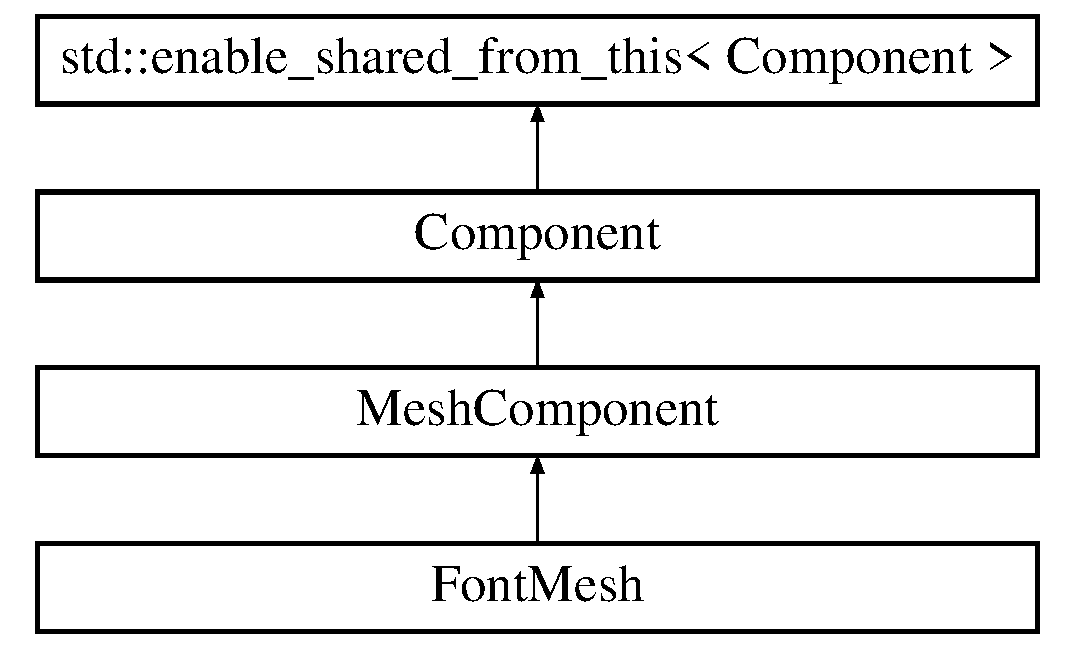
\includegraphics[height=4.000000cm]{class_font_mesh}
\end{center}
\end{figure}
\subsection*{Public Member Functions}
\begin{DoxyCompactItemize}
\item 
\hyperlink{class_font_mesh_aedfa6f6af9efdbe4c1fe400c128d74f8}{Font\+Mesh} ()
\item 
virtual \hyperlink{class_font_mesh_aa72cdbc114c4bd907cd3c80a0516eaa1}{$\sim$\+Font\+Mesh} ()
\item 
void \hyperlink{class_font_mesh_a9c8c08a909a3f1f8fe49427b714f49ea}{set\+Font} (shared\+\_\+ptr$<$ \hyperlink{class_font}{Font} $>$ font)
\item 
shared\+\_\+ptr$<$ \hyperlink{class_font}{Font} $>$ \hyperlink{class_font_mesh_a8ecf4127c1b8903e2d88e4010e5456c7}{get\+Font} ()
\item 
void \hyperlink{class_font_mesh_ab7b118065bcbaba9dad67fc472eb747d}{set\+Text} (string text)
\item 
string \hyperlink{class_font_mesh_a8be85c214ce53ce1c706a555c9c0c047}{get\+Text} ()
\item 
void \hyperlink{class_font_mesh_a604facf912301eb3443e5532a6f389d3}{create\+Mesh} ()
\item 
virtual shared\+\_\+ptr$<$ \hyperlink{class_component}{Component} $>$ \hyperlink{class_font_mesh_a4dd3900fcbb33aca326d1cd1871e7b92}{clone} () override
\item 
virtual shared\+\_\+ptr$<$ \hyperlink{class_component_description}{Component\+Description} $>$ \hyperlink{group__serialization__functions_gab58270595083da13e7c384f00318291b}{get\+Component\+Description} () override
\item 
virtual void \hyperlink{group__serialization__functions_ga76f4b78e5fd2adece4557f2a676f2c1b}{deserialize} (shared\+\_\+ptr$<$ \hyperlink{class_component_description}{Component\+Description} $>$ desc) override
\end{DoxyCompactItemize}
\subsection*{Additional Inherited Members}


\subsection{Detailed Description}
\hyperlink{class_font_mesh}{Font\+Mesh} is a \hyperlink{class_mesh_component}{Mesh\+Component}, meaning that it holds reference to a \hyperlink{class_mesh}{Mesh}. Unlike \hyperlink{class_mesh_filter}{Mesh\+Filter}, that makes reference to a \char`\"{}static\char`\"{} mesh, a file mesh, the \hyperlink{class_font_mesh}{Font\+Mesh} makes reference to a dynamic mesh, created according to the text it\textquotesingle{}s going to display. 

\subsection{Constructor \& Destructor Documentation}
\hypertarget{class_font_mesh_aedfa6f6af9efdbe4c1fe400c128d74f8}{}\index{Font\+Mesh@{Font\+Mesh}!Font\+Mesh@{Font\+Mesh}}
\index{Font\+Mesh@{Font\+Mesh}!Font\+Mesh@{Font\+Mesh}}
\subsubsection[{Font\+Mesh()}]{\setlength{\rightskip}{0pt plus 5cm}Font\+Mesh\+::\+Font\+Mesh (
\begin{DoxyParamCaption}
{}
\end{DoxyParamCaption}
)}\label{class_font_mesh_aedfa6f6af9efdbe4c1fe400c128d74f8}
Default Constructor \hypertarget{class_font_mesh_aa72cdbc114c4bd907cd3c80a0516eaa1}{}\index{Font\+Mesh@{Font\+Mesh}!````~Font\+Mesh@{$\sim$\+Font\+Mesh}}
\index{````~Font\+Mesh@{$\sim$\+Font\+Mesh}!Font\+Mesh@{Font\+Mesh}}
\subsubsection[{$\sim$\+Font\+Mesh()}]{\setlength{\rightskip}{0pt plus 5cm}Font\+Mesh\+::$\sim$\+Font\+Mesh (
\begin{DoxyParamCaption}
{}
\end{DoxyParamCaption}
)\hspace{0.3cm}{\ttfamily [virtual]}}\label{class_font_mesh_aa72cdbc114c4bd907cd3c80a0516eaa1}
Default Destructor. Virtual because it\textquotesingle{}s children class. 

\subsection{Member Function Documentation}
\hypertarget{class_font_mesh_a4dd3900fcbb33aca326d1cd1871e7b92}{}\index{Font\+Mesh@{Font\+Mesh}!clone@{clone}}
\index{clone@{clone}!Font\+Mesh@{Font\+Mesh}}
\subsubsection[{clone() override}]{\setlength{\rightskip}{0pt plus 5cm}shared\+\_\+ptr$<$ {\bf Component} $>$ Font\+Mesh\+::clone (
\begin{DoxyParamCaption}
{}
\end{DoxyParamCaption}
)\hspace{0.3cm}{\ttfamily [override]}, {\ttfamily [virtual]}}\label{class_font_mesh_a4dd3900fcbb33aca326d1cd1871e7b92}
Clones current component (Prototype Design Pattern) \begin{DoxyReturn}{Returns}
shared\+\_\+ptr to cloned \hyperlink{class_font_mesh}{Font\+Mesh} \hyperlink{class_component}{Component} 
\end{DoxyReturn}


Implements \hyperlink{class_mesh_component_ace2f1acdce65f1c37b56a5b3ef507e8d}{Mesh\+Component}.

\hypertarget{class_font_mesh_a604facf912301eb3443e5532a6f389d3}{}\index{Font\+Mesh@{Font\+Mesh}!create\+Mesh@{create\+Mesh}}
\index{create\+Mesh@{create\+Mesh}!Font\+Mesh@{Font\+Mesh}}
\subsubsection[{create\+Mesh()}]{\setlength{\rightskip}{0pt plus 5cm}void Font\+Mesh\+::create\+Mesh (
\begin{DoxyParamCaption}
{}
\end{DoxyParamCaption}
)}\label{class_font_mesh_a604facf912301eb3443e5532a6f389d3}
create the mesh according to the font and text \hypertarget{class_font_mesh_a8ecf4127c1b8903e2d88e4010e5456c7}{}\index{Font\+Mesh@{Font\+Mesh}!get\+Font@{get\+Font}}
\index{get\+Font@{get\+Font}!Font\+Mesh@{Font\+Mesh}}
\subsubsection[{get\+Font()}]{\setlength{\rightskip}{0pt plus 5cm}shared\+\_\+ptr$<$ {\bf Font} $>$ Font\+Mesh\+::get\+Font (
\begin{DoxyParamCaption}
{}
\end{DoxyParamCaption}
)}\label{class_font_mesh_a8ecf4127c1b8903e2d88e4010e5456c7}
font getter \hypertarget{class_font_mesh_a8be85c214ce53ce1c706a555c9c0c047}{}\index{Font\+Mesh@{Font\+Mesh}!get\+Text@{get\+Text}}
\index{get\+Text@{get\+Text}!Font\+Mesh@{Font\+Mesh}}
\subsubsection[{get\+Text()}]{\setlength{\rightskip}{0pt plus 5cm}string Font\+Mesh\+::get\+Text (
\begin{DoxyParamCaption}
{}
\end{DoxyParamCaption}
)}\label{class_font_mesh_a8be85c214ce53ce1c706a555c9c0c047}
text getter \hypertarget{class_font_mesh_a9c8c08a909a3f1f8fe49427b714f49ea}{}\index{Font\+Mesh@{Font\+Mesh}!set\+Font@{set\+Font}}
\index{set\+Font@{set\+Font}!Font\+Mesh@{Font\+Mesh}}
\subsubsection[{set\+Font(shared\+\_\+ptr$<$ Font $>$ font)}]{\setlength{\rightskip}{0pt plus 5cm}void Font\+Mesh\+::set\+Font (
\begin{DoxyParamCaption}
\item[{shared\+\_\+ptr$<$ {\bf Font} $>$}]{font}
\end{DoxyParamCaption}
)}\label{class_font_mesh_a9c8c08a909a3f1f8fe49427b714f49ea}
font setter \hypertarget{class_font_mesh_ab7b118065bcbaba9dad67fc472eb747d}{}\index{Font\+Mesh@{Font\+Mesh}!set\+Text@{set\+Text}}
\index{set\+Text@{set\+Text}!Font\+Mesh@{Font\+Mesh}}
\subsubsection[{set\+Text(string text)}]{\setlength{\rightskip}{0pt plus 5cm}void Font\+Mesh\+::set\+Text (
\begin{DoxyParamCaption}
\item[{string}]{text}
\end{DoxyParamCaption}
)}\label{class_font_mesh_ab7b118065bcbaba9dad67fc472eb747d}
text setter 

The documentation for this class was generated from the following files\+:\begin{DoxyCompactItemize}
\item 
/\+Users/guilherme\+\_\+cunha/\+Dev/\+G\+I\+T\+H\+U\+B/\+G\+U\+Inity/\+Source/Font\+Mesh.\+hpp\item 
/\+Users/guilherme\+\_\+cunha/\+Dev/\+G\+I\+T\+H\+U\+B/\+G\+U\+Inity/\+Source/Font\+Mesh.\+cpp\end{DoxyCompactItemize}

\hypertarget{class_game}{}\section{Game Class Reference}
\label{class_game}\index{Game@{Game}}
Inheritance diagram for Game\+:\begin{figure}[H]
\begin{center}
\leavevmode
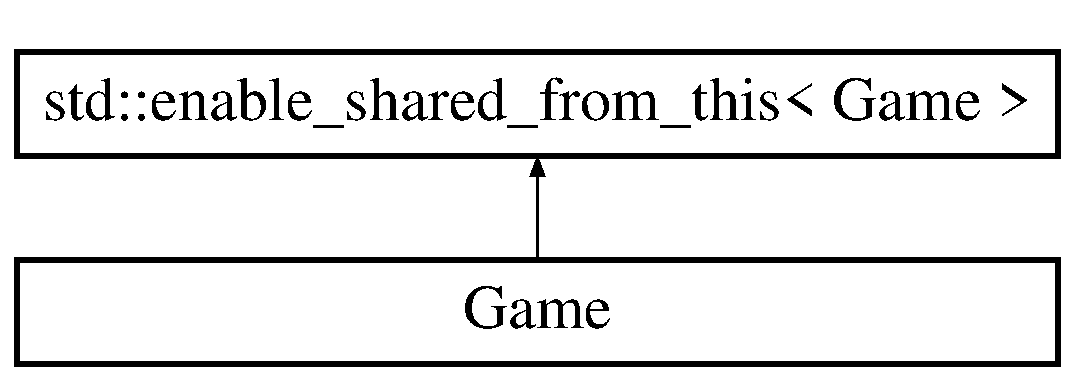
\includegraphics[height=2.000000cm]{class_game}
\end{center}
\end{figure}
\subsection*{Public Member Functions}
\begin{DoxyCompactItemize}
\item 
\hypertarget{class_game_ad63cb8a7a3091b9542186e4c1128a59b}{}void {\bfseries update} (float delta\+Seconds)\label{class_game_ad63cb8a7a3091b9542186e4c1128a59b}

\item 
\hypertarget{class_game_a6f3a33940524b6ba9d83f627ccb14bbf}{}void {\bfseries init} ()\label{class_game_a6f3a33940524b6ba9d83f627ccb14bbf}

\item 
\hypertarget{class_game_aee1b95e6fd0cb0f441c3b7cef73b1abe}{}void {\bfseries shutdown} ()\label{class_game_aee1b95e6fd0cb0f441c3b7cef73b1abe}

\end{DoxyCompactItemize}
\subsection*{Public Attributes}
\begin{DoxyCompactItemize}
\item 
\hypertarget{class_game_a550e03843cecc2678a6d42b3cc656d7b}{}Px\+Scene $\ast$ {\bfseries physics\+Scene}\label{class_game_a550e03843cecc2678a6d42b3cc656d7b}

\end{DoxyCompactItemize}
\subsection*{Static Public Attributes}
\begin{DoxyCompactItemize}
\item 
\hypertarget{class_game_aa4b3e2d2e9914ea12726c5f26ef7023a}{}static shared\+\_\+ptr$<$ \hyperlink{class_world}{World} $>$ {\bfseries world}\label{class_game_aa4b3e2d2e9914ea12726c5f26ef7023a}

\end{DoxyCompactItemize}


The documentation for this class was generated from the following files\+:\begin{DoxyCompactItemize}
\item 
/\+Users/guilherme\+\_\+cunha/\+Dev/\+G\+I\+T\+H\+U\+B/\+G\+U\+Inity/\+Source/Game.\+hpp\item 
/\+Users/guilherme\+\_\+cunha/\+Dev/\+G\+I\+T\+H\+U\+B/\+G\+U\+Inity/\+Source/Game.\+cpp\end{DoxyCompactItemize}

\hypertarget{class_g_l_f_w_graphics_system}{}\section{G\+L\+F\+W\+Graphics\+System Class Reference}
\label{class_g_l_f_w_graphics_system}\index{G\+L\+F\+W\+Graphics\+System@{G\+L\+F\+W\+Graphics\+System}}
Inheritance diagram for G\+L\+F\+W\+Graphics\+System\+:\begin{figure}[H]
\begin{center}
\leavevmode
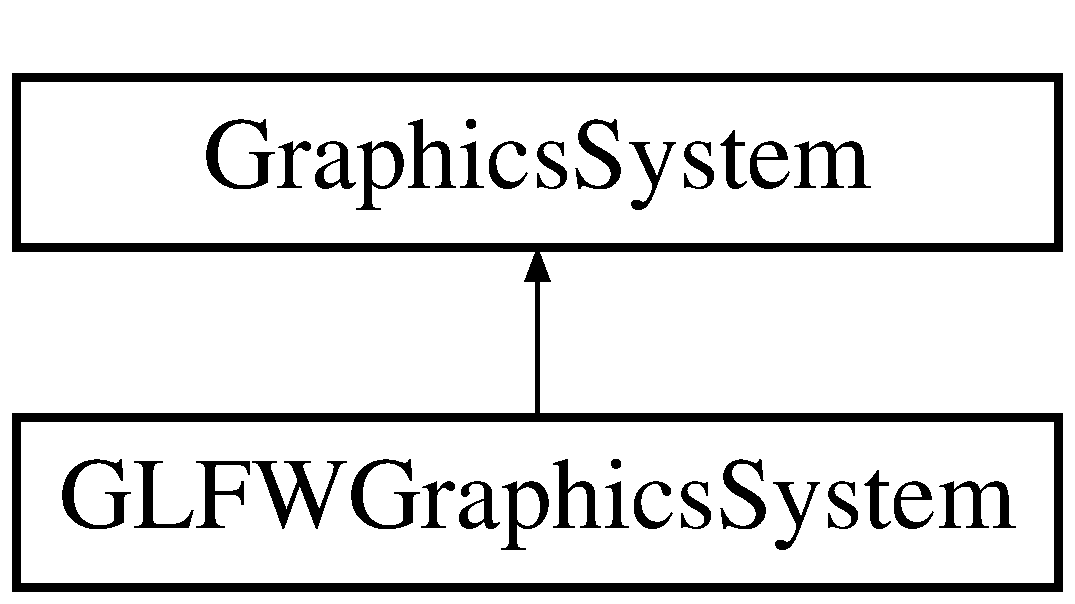
\includegraphics[height=2.000000cm]{class_g_l_f_w_graphics_system}
\end{center}
\end{figure}
\subsection*{Public Member Functions}
\begin{DoxyCompactItemize}
\item 
virtual \hyperlink{class_g_l_f_w_graphics_system_ad73c55b92fcbd41921d7929f7332e8af}{$\sim$\+G\+L\+F\+W\+Graphics\+System} ()
\item 
\hyperlink{class_g_l_f_w_graphics_system_a0cc238f56cef77f89e5b09b5a9b46cb6}{G\+L\+F\+W\+Graphics\+System} ()
\item 
virtual int \hyperlink{class_g_l_f_w_graphics_system_a4cba85b32cd751aab2f5a84c01199953}{init} (int width, int height) override
\item 
virtual void \hyperlink{class_g_l_f_w_graphics_system_ab12358c2a7034dcf75df074fbe4d86d4}{shutdown} () override
\item 
virtual void \hyperlink{class_g_l_f_w_graphics_system_a52ef8cd44b2b45828452626d9e0b54d6}{swap} () override
\item 
virtual void \hyperlink{class_g_l_f_w_graphics_system_a84767a0209a04f598b866048e04b2035}{clear} () override
\item 
virtual void \hyperlink{class_g_l_f_w_graphics_system_a446723c2cad999498d013f71ab8e570f}{create\+Debug\+Shader} () override
\item 
virtual int \hyperlink{class_g_l_f_w_graphics_system_a8c31a0ea165e6c9cbd0e0c656342a200}{get\+Screen\+Width} () override
\item 
virtual int \hyperlink{class_g_l_f_w_graphics_system_ab6b0c31d3d5fb238a19c645630b87543}{get\+Screen\+Height} () override
\item 
virtual void \hyperlink{class_g_l_f_w_graphics_system_a606c4e6e8e53084d3d23bc7bbcdfc228}{render} (shared\+\_\+ptr$<$ \hyperlink{class_camera}{Camera} $>$ camera, const physx\+::\+Px\+Render\+Buffer \&rb, const glm\+::vec4 \&color) override
\item 
virtual void \hyperlink{class_g_l_f_w_graphics_system_a2cde625e8606c2905d7728f2cadf7371}{render} (shared\+\_\+ptr$<$ \hyperlink{class_camera}{Camera} $>$ camera, vector$<$ shared\+\_\+ptr$<$ \hyperlink{class_mesh_renderer}{Mesh\+Renderer} $>$$>$ \&renderers, vector$<$ shared\+\_\+ptr$<$ \hyperlink{class_light}{Light} $>$$>$ \&lights) override
\item 
virtual void \hyperlink{class_g_l_f_w_graphics_system_a8ebfaa6c98ba4a92618835de8966e8b9}{render\+G\+U\+I} (vector$<$ shared\+\_\+ptr$<$ U\+I\+Widget $>$$>$ ui\+Widget\+Vector) override
\item 
virtual void \hyperlink{class_g_l_f_w_graphics_system_a6b40d73f5eea98cebe77e51f7cba8f6c}{generate\+Vertex\+Arrays} (const G\+Luint id, G\+Luint \&vao) override
\item 
virtual void \hyperlink{class_g_l_f_w_graphics_system_a22f72c31efab822c4d958a217f61340c}{generate\+Buffer} (const G\+Luint id, G\+Luint \&bo, G\+Lenum type, int size, void $\ast$data\+Pointer, G\+Lenum draw\+Type) override
\item 
virtual void \hyperlink{class_g_l_f_w_graphics_system_aa7d78cc01b84a7ab6d90343d5adf4432}{delete\+Buffer} (G\+Luint size, G\+Luint \&bo) override
\item 
virtual G\+Luint \hyperlink{class_g_l_f_w_graphics_system_a366ee287cdf55396fdd846e59235f2ea}{create\+Shader} (G\+Lenum shader\+Type) override
\item 
virtual void \hyperlink{class_g_l_f_w_graphics_system_a9a791ee2a7a5465cff955bc03451c998}{delete\+Shader} (G\+Luint shader\+I\+D) override
\item 
virtual void \hyperlink{class_g_l_f_w_graphics_system_a87e2461accc1340e6ebc568729a8019a}{compile\+Shader} (G\+Luint shader\+I\+D, G\+Luint size, const char $\ast$data\+Pointer) override
\item 
virtual void \hyperlink{class_g_l_f_w_graphics_system_a1b993a6ed176405ba676d2f5569d373e}{attach\+And\+Link\+Shader} (G\+Luint Program\+I\+D, G\+Luint Vertex\+Shader\+I\+D, G\+Luint Fragment\+Shader\+I\+D) override
\item 
virtual G\+Luint \hyperlink{class_g_l_f_w_graphics_system_ac188b290e2647010d1ad8c0a07d63cf0}{create\+Shader\+Program} () override
\item 
virtual G\+Lint \hyperlink{class_g_l_f_w_graphics_system_ad7f9cc29bfe40cf3d498962fd50ccc16}{get\+Uniform\+Location} (G\+Luint program\+I\+D, const char $\ast$name) override
\item 
virtual shared\+\_\+ptr$<$ \hyperlink{class_texture}{Texture} $>$ \hyperlink{class_g_l_f_w_graphics_system_ad5b712896c2c8819ff3ea88ab16cf8ce}{get\+Default\+Texture} () override
\item 
void \hyperlink{class_g_l_f_w_graphics_system_afae3be496cd9d8fdafc7bd0809f38039}{disable\+Non\+Used\+Textures} (int n\+Textures) const 
\item 
\hypertarget{class_g_l_f_w_graphics_system_aa695e9c03f212418751abd904cd36159}{}bool {\bfseries set\+Uniform4fv} (const G\+Luint \&shader\+Program, const G\+Lchar $\ast$uniform\+Name, int count, G\+Lfloat $\ast$value)\label{class_g_l_f_w_graphics_system_aa695e9c03f212418751abd904cd36159}

\item 
\hypertarget{class_g_l_f_w_graphics_system_af650ad61b843a8d8b58ff87adba07a7f}{}bool {\bfseries set\+Uniform3fv} (const G\+Luint \&shader\+Program, const G\+Lchar $\ast$uniform\+Name, int count, G\+Lfloat $\ast$value)\label{class_g_l_f_w_graphics_system_af650ad61b843a8d8b58ff87adba07a7f}

\item 
\hypertarget{class_g_l_f_w_graphics_system_a36eaf8614118693c0ceb299be56c119b}{}bool {\bfseries set\+Uniform1f} (const G\+Luint \&shader\+Program, const G\+Lchar $\ast$uniform\+Name, G\+Lfloat value)\label{class_g_l_f_w_graphics_system_a36eaf8614118693c0ceb299be56c119b}

\item 
\hypertarget{class_g_l_f_w_graphics_system_ad7b50419fe5eba7b389e94a673942130}{}bool {\bfseries set\+Uniform\+Matrix4fv} (const G\+Luint \&shader\+Program, const G\+Lchar $\ast$uniform\+Name, int count, G\+Lboolean transpose, G\+Lfloat $\ast$value)\label{class_g_l_f_w_graphics_system_ad7b50419fe5eba7b389e94a673942130}

\end{DoxyCompactItemize}
\subsection*{Additional Inherited Members}


\subsection{Constructor \& Destructor Documentation}
\hypertarget{class_g_l_f_w_graphics_system_ad73c55b92fcbd41921d7929f7332e8af}{}\index{G\+L\+F\+W\+Graphics\+System@{G\+L\+F\+W\+Graphics\+System}!````~G\+L\+F\+W\+Graphics\+System@{$\sim$\+G\+L\+F\+W\+Graphics\+System}}
\index{````~G\+L\+F\+W\+Graphics\+System@{$\sim$\+G\+L\+F\+W\+Graphics\+System}!G\+L\+F\+W\+Graphics\+System@{G\+L\+F\+W\+Graphics\+System}}
\subsubsection[{$\sim$\+G\+L\+F\+W\+Graphics\+System()}]{\setlength{\rightskip}{0pt plus 5cm}virtual G\+L\+F\+W\+Graphics\+System\+::$\sim$\+G\+L\+F\+W\+Graphics\+System (
\begin{DoxyParamCaption}
{}
\end{DoxyParamCaption}
)\hspace{0.3cm}{\ttfamily [inline]}, {\ttfamily [virtual]}}\label{class_g_l_f_w_graphics_system_ad73c55b92fcbd41921d7929f7332e8af}
Default Destructor \hypertarget{class_g_l_f_w_graphics_system_a0cc238f56cef77f89e5b09b5a9b46cb6}{}\index{G\+L\+F\+W\+Graphics\+System@{G\+L\+F\+W\+Graphics\+System}!G\+L\+F\+W\+Graphics\+System@{G\+L\+F\+W\+Graphics\+System}}
\index{G\+L\+F\+W\+Graphics\+System@{G\+L\+F\+W\+Graphics\+System}!G\+L\+F\+W\+Graphics\+System@{G\+L\+F\+W\+Graphics\+System}}
\subsubsection[{G\+L\+F\+W\+Graphics\+System()}]{\setlength{\rightskip}{0pt plus 5cm}G\+L\+F\+W\+Graphics\+System\+::\+G\+L\+F\+W\+Graphics\+System (
\begin{DoxyParamCaption}
{}
\end{DoxyParamCaption}
)\hspace{0.3cm}{\ttfamily [inline]}}\label{class_g_l_f_w_graphics_system_a0cc238f56cef77f89e5b09b5a9b46cb6}
Default Constructor. Virtual because it inherits from \hyperlink{class_graphics_system}{Graphics\+System} 

\subsection{Member Function Documentation}
\hypertarget{class_g_l_f_w_graphics_system_a1b993a6ed176405ba676d2f5569d373e}{}\index{G\+L\+F\+W\+Graphics\+System@{G\+L\+F\+W\+Graphics\+System}!attach\+And\+Link\+Shader@{attach\+And\+Link\+Shader}}
\index{attach\+And\+Link\+Shader@{attach\+And\+Link\+Shader}!G\+L\+F\+W\+Graphics\+System@{G\+L\+F\+W\+Graphics\+System}}
\subsubsection[{attach\+And\+Link\+Shader(\+G\+Luint Program\+I\+D, G\+Luint Vertex\+Shader\+I\+D, G\+Luint Fragment\+Shader\+I\+D) override}]{\setlength{\rightskip}{0pt plus 5cm}void G\+L\+F\+W\+Graphics\+System\+::attach\+And\+Link\+Shader (
\begin{DoxyParamCaption}
\item[{G\+Luint}]{Program\+I\+D, }
\item[{G\+Luint}]{Vertex\+Shader\+I\+D, }
\item[{G\+Luint}]{Fragment\+Shader\+I\+D}
\end{DoxyParamCaption}
)\hspace{0.3cm}{\ttfamily [override]}, {\ttfamily [virtual]}}\label{class_g_l_f_w_graphics_system_a1b993a6ed176405ba676d2f5569d373e}
Merge Vertex\+Shader and Fragment\+Shader to one 

Implements \hyperlink{class_graphics_system_aa166087f35ee2af8a9c9a45bd4a6103d}{Graphics\+System}.

\hypertarget{class_g_l_f_w_graphics_system_a84767a0209a04f598b866048e04b2035}{}\index{G\+L\+F\+W\+Graphics\+System@{G\+L\+F\+W\+Graphics\+System}!clear@{clear}}
\index{clear@{clear}!G\+L\+F\+W\+Graphics\+System@{G\+L\+F\+W\+Graphics\+System}}
\subsubsection[{clear() override}]{\setlength{\rightskip}{0pt plus 5cm}void G\+L\+F\+W\+Graphics\+System\+::clear (
\begin{DoxyParamCaption}
{}
\end{DoxyParamCaption}
)\hspace{0.3cm}{\ttfamily [override]}, {\ttfamily [virtual]}}\label{class_g_l_f_w_graphics_system_a84767a0209a04f598b866048e04b2035}
Clear buffers 

Implements \hyperlink{class_graphics_system_acb34692fa9eb3c03c8a80ddfb6ea1e3f}{Graphics\+System}.

\hypertarget{class_g_l_f_w_graphics_system_a87e2461accc1340e6ebc568729a8019a}{}\index{G\+L\+F\+W\+Graphics\+System@{G\+L\+F\+W\+Graphics\+System}!compile\+Shader@{compile\+Shader}}
\index{compile\+Shader@{compile\+Shader}!G\+L\+F\+W\+Graphics\+System@{G\+L\+F\+W\+Graphics\+System}}
\subsubsection[{compile\+Shader(\+G\+Luint shader\+I\+D, G\+Luint size, const char $\ast$data\+Pointer) override}]{\setlength{\rightskip}{0pt plus 5cm}void G\+L\+F\+W\+Graphics\+System\+::compile\+Shader (
\begin{DoxyParamCaption}
\item[{G\+Luint}]{shader\+I\+D, }
\item[{G\+Luint}]{size, }
\item[{const char $\ast$}]{data\+Pointer}
\end{DoxyParamCaption}
)\hspace{0.3cm}{\ttfamily [override]}, {\ttfamily [virtual]}}\label{class_g_l_f_w_graphics_system_a87e2461accc1340e6ebc568729a8019a}
Compile the shader 

Implements \hyperlink{class_graphics_system_ad287e692cbaab0fd5560df2f0cd98fc7}{Graphics\+System}.

\hypertarget{class_g_l_f_w_graphics_system_a446723c2cad999498d013f71ab8e570f}{}\index{G\+L\+F\+W\+Graphics\+System@{G\+L\+F\+W\+Graphics\+System}!create\+Debug\+Shader@{create\+Debug\+Shader}}
\index{create\+Debug\+Shader@{create\+Debug\+Shader}!G\+L\+F\+W\+Graphics\+System@{G\+L\+F\+W\+Graphics\+System}}
\subsubsection[{create\+Debug\+Shader() override}]{\setlength{\rightskip}{0pt plus 5cm}void G\+L\+F\+W\+Graphics\+System\+::create\+Debug\+Shader (
\begin{DoxyParamCaption}
{}
\end{DoxyParamCaption}
)\hspace{0.3cm}{\ttfamily [override]}, {\ttfamily [virtual]}}\label{class_g_l_f_w_graphics_system_a446723c2cad999498d013f71ab8e570f}
create debug shader to display \hyperlink{class_physics}{Physics} information on the screen 

Implements \hyperlink{class_graphics_system_a235c9266682e6521135003593409b92e}{Graphics\+System}.

\hypertarget{class_g_l_f_w_graphics_system_a366ee287cdf55396fdd846e59235f2ea}{}\index{G\+L\+F\+W\+Graphics\+System@{G\+L\+F\+W\+Graphics\+System}!create\+Shader@{create\+Shader}}
\index{create\+Shader@{create\+Shader}!G\+L\+F\+W\+Graphics\+System@{G\+L\+F\+W\+Graphics\+System}}
\subsubsection[{create\+Shader(\+G\+Lenum shader\+Type) override}]{\setlength{\rightskip}{0pt plus 5cm}G\+Luint G\+L\+F\+W\+Graphics\+System\+::create\+Shader (
\begin{DoxyParamCaption}
\item[{G\+Lenum}]{shader\+Type}
\end{DoxyParamCaption}
)\hspace{0.3cm}{\ttfamily [override]}, {\ttfamily [virtual]}}\label{class_g_l_f_w_graphics_system_a366ee287cdf55396fdd846e59235f2ea}
Creates a new shader 

Implements \hyperlink{class_graphics_system_a352afd81ae42f6415b4e28ff445e5d45}{Graphics\+System}.

\hypertarget{class_g_l_f_w_graphics_system_ac188b290e2647010d1ad8c0a07d63cf0}{}\index{G\+L\+F\+W\+Graphics\+System@{G\+L\+F\+W\+Graphics\+System}!create\+Shader\+Program@{create\+Shader\+Program}}
\index{create\+Shader\+Program@{create\+Shader\+Program}!G\+L\+F\+W\+Graphics\+System@{G\+L\+F\+W\+Graphics\+System}}
\subsubsection[{create\+Shader\+Program() override}]{\setlength{\rightskip}{0pt plus 5cm}G\+Luint G\+L\+F\+W\+Graphics\+System\+::create\+Shader\+Program (
\begin{DoxyParamCaption}
{}
\end{DoxyParamCaption}
)\hspace{0.3cm}{\ttfamily [override]}, {\ttfamily [virtual]}}\label{class_g_l_f_w_graphics_system_ac188b290e2647010d1ad8c0a07d63cf0}
Creates a new shader program

Merge Vertex\+Shader and Fragment\+Shader to one 

Implements \hyperlink{class_graphics_system_a6c8d55818a976c504faf291c78f51ca5}{Graphics\+System}.

\hypertarget{class_g_l_f_w_graphics_system_aa7d78cc01b84a7ab6d90343d5adf4432}{}\index{G\+L\+F\+W\+Graphics\+System@{G\+L\+F\+W\+Graphics\+System}!delete\+Buffer@{delete\+Buffer}}
\index{delete\+Buffer@{delete\+Buffer}!G\+L\+F\+W\+Graphics\+System@{G\+L\+F\+W\+Graphics\+System}}
\subsubsection[{delete\+Buffer(\+G\+Luint size, G\+Luint \&bo) override}]{\setlength{\rightskip}{0pt plus 5cm}void G\+L\+F\+W\+Graphics\+System\+::delete\+Buffer (
\begin{DoxyParamCaption}
\item[{G\+Luint}]{size, }
\item[{G\+Luint \&}]{bo}
\end{DoxyParamCaption}
)\hspace{0.3cm}{\ttfamily [override]}, {\ttfamily [virtual]}}\label{class_g_l_f_w_graphics_system_aa7d78cc01b84a7ab6d90343d5adf4432}
Release buffer 

Implements \hyperlink{class_graphics_system_a526e6b5fea898f4ac06ef0d0ab7b9d67}{Graphics\+System}.

\hypertarget{class_g_l_f_w_graphics_system_a9a791ee2a7a5465cff955bc03451c998}{}\index{G\+L\+F\+W\+Graphics\+System@{G\+L\+F\+W\+Graphics\+System}!delete\+Shader@{delete\+Shader}}
\index{delete\+Shader@{delete\+Shader}!G\+L\+F\+W\+Graphics\+System@{G\+L\+F\+W\+Graphics\+System}}
\subsubsection[{delete\+Shader(\+G\+Luint shader\+I\+D) override}]{\setlength{\rightskip}{0pt plus 5cm}void G\+L\+F\+W\+Graphics\+System\+::delete\+Shader (
\begin{DoxyParamCaption}
\item[{G\+Luint}]{shader\+I\+D}
\end{DoxyParamCaption}
)\hspace{0.3cm}{\ttfamily [override]}, {\ttfamily [virtual]}}\label{class_g_l_f_w_graphics_system_a9a791ee2a7a5465cff955bc03451c998}
Release shader 

Implements \hyperlink{class_graphics_system_ab56e3749349d38b97fdb5fecd5a184e8}{Graphics\+System}.

\hypertarget{class_g_l_f_w_graphics_system_afae3be496cd9d8fdafc7bd0809f38039}{}\index{G\+L\+F\+W\+Graphics\+System@{G\+L\+F\+W\+Graphics\+System}!disable\+Non\+Used\+Textures@{disable\+Non\+Used\+Textures}}
\index{disable\+Non\+Used\+Textures@{disable\+Non\+Used\+Textures}!G\+L\+F\+W\+Graphics\+System@{G\+L\+F\+W\+Graphics\+System}}
\subsubsection[{disable\+Non\+Used\+Textures(int n\+Textures) const }]{\setlength{\rightskip}{0pt plus 5cm}void G\+L\+F\+W\+Graphics\+System\+::disable\+Non\+Used\+Textures (
\begin{DoxyParamCaption}
\item[{int}]{n\+Textures}
\end{DoxyParamCaption}
) const}\label{class_g_l_f_w_graphics_system_afae3be496cd9d8fdafc7bd0809f38039}
Disable Textures that have are not needed for the current draw call

Disable Textures that are not needed for the current draw call \hypertarget{class_g_l_f_w_graphics_system_a22f72c31efab822c4d958a217f61340c}{}\index{G\+L\+F\+W\+Graphics\+System@{G\+L\+F\+W\+Graphics\+System}!generate\+Buffer@{generate\+Buffer}}
\index{generate\+Buffer@{generate\+Buffer}!G\+L\+F\+W\+Graphics\+System@{G\+L\+F\+W\+Graphics\+System}}
\subsubsection[{generate\+Buffer(const G\+Luint id, G\+Luint \&bo, G\+Lenum type, int size, void $\ast$data\+Pointer, G\+Lenum draw\+Type) override}]{\setlength{\rightskip}{0pt plus 5cm}void G\+L\+F\+W\+Graphics\+System\+::generate\+Buffer (
\begin{DoxyParamCaption}
\item[{const G\+Luint}]{size, }
\item[{G\+Luint \&}]{bo, }
\item[{G\+Lenum}]{type, }
\item[{int}]{data\+Size, }
\item[{void $\ast$}]{data\+Pointer, }
\item[{G\+Lenum}]{draw\+Type}
\end{DoxyParamCaption}
)\hspace{0.3cm}{\ttfamily [override]}, {\ttfamily [virtual]}}\label{class_g_l_f_w_graphics_system_a22f72c31efab822c4d958a217f61340c}
Generates a new Buffer Array 

Implements \hyperlink{class_graphics_system_a6ca91563b69a554462fccbcfff2d6a70}{Graphics\+System}.

\hypertarget{class_g_l_f_w_graphics_system_a6b40d73f5eea98cebe77e51f7cba8f6c}{}\index{G\+L\+F\+W\+Graphics\+System@{G\+L\+F\+W\+Graphics\+System}!generate\+Vertex\+Arrays@{generate\+Vertex\+Arrays}}
\index{generate\+Vertex\+Arrays@{generate\+Vertex\+Arrays}!G\+L\+F\+W\+Graphics\+System@{G\+L\+F\+W\+Graphics\+System}}
\subsubsection[{generate\+Vertex\+Arrays(const G\+Luint id, G\+Luint \&vao) override}]{\setlength{\rightskip}{0pt plus 5cm}void G\+L\+F\+W\+Graphics\+System\+::generate\+Vertex\+Arrays (
\begin{DoxyParamCaption}
\item[{const G\+Luint}]{id, }
\item[{G\+Luint \&}]{vao}
\end{DoxyParamCaption}
)\hspace{0.3cm}{\ttfamily [override]}, {\ttfamily [virtual]}}\label{class_g_l_f_w_graphics_system_a6b40d73f5eea98cebe77e51f7cba8f6c}
Generates a new Vertex Array -\/ Used for mesh vertice data 

Implements \hyperlink{class_graphics_system_a32ab75f493e9037c83b718f5ccb11500}{Graphics\+System}.

\hypertarget{class_g_l_f_w_graphics_system_ad5b712896c2c8819ff3ea88ab16cf8ce}{}\index{G\+L\+F\+W\+Graphics\+System@{G\+L\+F\+W\+Graphics\+System}!get\+Default\+Texture@{get\+Default\+Texture}}
\index{get\+Default\+Texture@{get\+Default\+Texture}!G\+L\+F\+W\+Graphics\+System@{G\+L\+F\+W\+Graphics\+System}}
\subsubsection[{get\+Default\+Texture() override}]{\setlength{\rightskip}{0pt plus 5cm}shared\+\_\+ptr$<$ {\bf Texture} $>$ G\+L\+F\+W\+Graphics\+System\+::get\+Default\+Texture (
\begin{DoxyParamCaption}
{}
\end{DoxyParamCaption}
)\hspace{0.3cm}{\ttfamily [override]}, {\ttfamily [virtual]}}\label{class_g_l_f_w_graphics_system_ad5b712896c2c8819ff3ea88ab16cf8ce}
Gets the uniform location for a string in a shader 

Implements \hyperlink{class_graphics_system}{Graphics\+System}.

\hypertarget{class_g_l_f_w_graphics_system_ab6b0c31d3d5fb238a19c645630b87543}{}\index{G\+L\+F\+W\+Graphics\+System@{G\+L\+F\+W\+Graphics\+System}!get\+Screen\+Height@{get\+Screen\+Height}}
\index{get\+Screen\+Height@{get\+Screen\+Height}!G\+L\+F\+W\+Graphics\+System@{G\+L\+F\+W\+Graphics\+System}}
\subsubsection[{get\+Screen\+Height() override}]{\setlength{\rightskip}{0pt plus 5cm}int G\+L\+F\+W\+Graphics\+System\+::get\+Screen\+Height (
\begin{DoxyParamCaption}
{}
\end{DoxyParamCaption}
)\hspace{0.3cm}{\ttfamily [override]}, {\ttfamily [virtual]}}\label{class_g_l_f_w_graphics_system_ab6b0c31d3d5fb238a19c645630b87543}
screen height Getter 

Implements \hyperlink{class_graphics_system_a056ee98bac2643fabd540f0541707cce}{Graphics\+System}.

\hypertarget{class_g_l_f_w_graphics_system_a8c31a0ea165e6c9cbd0e0c656342a200}{}\index{G\+L\+F\+W\+Graphics\+System@{G\+L\+F\+W\+Graphics\+System}!get\+Screen\+Width@{get\+Screen\+Width}}
\index{get\+Screen\+Width@{get\+Screen\+Width}!G\+L\+F\+W\+Graphics\+System@{G\+L\+F\+W\+Graphics\+System}}
\subsubsection[{get\+Screen\+Width() override}]{\setlength{\rightskip}{0pt plus 5cm}int G\+L\+F\+W\+Graphics\+System\+::get\+Screen\+Width (
\begin{DoxyParamCaption}
{}
\end{DoxyParamCaption}
)\hspace{0.3cm}{\ttfamily [override]}, {\ttfamily [virtual]}}\label{class_g_l_f_w_graphics_system_a8c31a0ea165e6c9cbd0e0c656342a200}
screen width Getter 

Implements \hyperlink{class_graphics_system_a9ebe243b7671cf0a4486bb9ae1f458f9}{Graphics\+System}.

\hypertarget{class_g_l_f_w_graphics_system_ad7f9cc29bfe40cf3d498962fd50ccc16}{}\index{G\+L\+F\+W\+Graphics\+System@{G\+L\+F\+W\+Graphics\+System}!get\+Uniform\+Location@{get\+Uniform\+Location}}
\index{get\+Uniform\+Location@{get\+Uniform\+Location}!G\+L\+F\+W\+Graphics\+System@{G\+L\+F\+W\+Graphics\+System}}
\subsubsection[{get\+Uniform\+Location(\+G\+Luint program\+I\+D, const char $\ast$name) override}]{\setlength{\rightskip}{0pt plus 5cm}G\+Lint G\+L\+F\+W\+Graphics\+System\+::get\+Uniform\+Location (
\begin{DoxyParamCaption}
\item[{G\+Luint}]{program\+I\+D, }
\item[{const char $\ast$}]{name}
\end{DoxyParamCaption}
)\hspace{0.3cm}{\ttfamily [override]}, {\ttfamily [virtual]}}\label{class_g_l_f_w_graphics_system_ad7f9cc29bfe40cf3d498962fd50ccc16}
Gets the uniform location for a string in a shader 

Implements \hyperlink{class_graphics_system_a32d2b6a92081eb59245849777f82f935}{Graphics\+System}.

\hypertarget{class_g_l_f_w_graphics_system_a4cba85b32cd751aab2f5a84c01199953}{}\index{G\+L\+F\+W\+Graphics\+System@{G\+L\+F\+W\+Graphics\+System}!init@{init}}
\index{init@{init}!G\+L\+F\+W\+Graphics\+System@{G\+L\+F\+W\+Graphics\+System}}
\subsubsection[{init(int width, int height) override}]{\setlength{\rightskip}{0pt plus 5cm}int G\+L\+F\+W\+Graphics\+System\+::init (
\begin{DoxyParamCaption}
\item[{int}]{width, }
\item[{int}]{height}
\end{DoxyParamCaption}
)\hspace{0.3cm}{\ttfamily [override]}, {\ttfamily [virtual]}}\label{class_g_l_f_w_graphics_system_a4cba85b32cd751aab2f5a84c01199953}
Initialize the system, create the window and such 

Implements \hyperlink{class_graphics_system_a7cdc16551f8da01c5271dfb64f807726}{Graphics\+System}.

\hypertarget{class_g_l_f_w_graphics_system_a606c4e6e8e53084d3d23bc7bbcdfc228}{}\index{G\+L\+F\+W\+Graphics\+System@{G\+L\+F\+W\+Graphics\+System}!render@{render}}
\index{render@{render}!G\+L\+F\+W\+Graphics\+System@{G\+L\+F\+W\+Graphics\+System}}
\subsubsection[{render(shared\+\_\+ptr$<$ Camera $>$ camera, const physx\+::\+Px\+Render\+Buffer \&rb, const glm\+::vec4 \&color) override}]{\setlength{\rightskip}{0pt plus 5cm}void G\+L\+F\+W\+Graphics\+System\+::render (
\begin{DoxyParamCaption}
\item[{shared\+\_\+ptr$<$ {\bf Camera} $>$}]{camera, }
\item[{const physx\+::\+Px\+Render\+Buffer \&}]{rb, }
\item[{const glm\+::vec4 \&}]{color}
\end{DoxyParamCaption}
)\hspace{0.3cm}{\ttfamily [override]}, {\ttfamily [virtual]}}\label{class_g_l_f_w_graphics_system_a606c4e6e8e53084d3d23bc7bbcdfc228}
Renders \hyperlink{class_physics}{Physics} information on screen from the camera point of view 

Implements \hyperlink{class_graphics_system_a60e5c663c8b19a5fee37e40ef347e86e}{Graphics\+System}.

\hypertarget{class_g_l_f_w_graphics_system_a2cde625e8606c2905d7728f2cadf7371}{}\index{G\+L\+F\+W\+Graphics\+System@{G\+L\+F\+W\+Graphics\+System}!render@{render}}
\index{render@{render}!G\+L\+F\+W\+Graphics\+System@{G\+L\+F\+W\+Graphics\+System}}
\subsubsection[{render(shared\+\_\+ptr$<$ Camera $>$ camera, vector$<$ shared\+\_\+ptr$<$ Mesh\+Renderer $>$$>$ \&renderers, vector$<$ shared\+\_\+ptr$<$ Light $>$$>$ \&lights) override}]{\setlength{\rightskip}{0pt plus 5cm}void G\+L\+F\+W\+Graphics\+System\+::render (
\begin{DoxyParamCaption}
\item[{shared\+\_\+ptr$<$ {\bf Camera} $>$}]{camera, }
\item[{vector$<$ shared\+\_\+ptr$<$ {\bf Mesh\+Renderer} $>$$>$ \&}]{renderers, }
\item[{vector$<$ shared\+\_\+ptr$<$ {\bf Light} $>$$>$ \&}]{lights}
\end{DoxyParamCaption}
)\hspace{0.3cm}{\ttfamily [override]}, {\ttfamily [virtual]}}\label{class_g_l_f_w_graphics_system_a2cde625e8606c2905d7728f2cadf7371}
Renders meshes on the screen from the camera point of view 

Implements \hyperlink{class_graphics_system_a7fdefc85d986133bc43885f863cc9c7c}{Graphics\+System}.

\hypertarget{class_g_l_f_w_graphics_system_a8ebfaa6c98ba4a92618835de8966e8b9}{}\index{G\+L\+F\+W\+Graphics\+System@{G\+L\+F\+W\+Graphics\+System}!render\+G\+U\+I@{render\+G\+U\+I}}
\index{render\+G\+U\+I@{render\+G\+U\+I}!G\+L\+F\+W\+Graphics\+System@{G\+L\+F\+W\+Graphics\+System}}
\subsubsection[{render\+G\+U\+I(vector$<$ shared\+\_\+ptr$<$ U\+I\+Widget $>$$>$ ui\+Widget\+Vector) override}]{\setlength{\rightskip}{0pt plus 5cm}void G\+L\+F\+W\+Graphics\+System\+::render\+G\+U\+I (
\begin{DoxyParamCaption}
\item[{vector$<$ shared\+\_\+ptr$<$ U\+I\+Widget $>$$>$}]{ui\+Widget\+Vector}
\end{DoxyParamCaption}
)\hspace{0.3cm}{\ttfamily [override]}, {\ttfamily [virtual]}}\label{class_g_l_f_w_graphics_system_a8ebfaa6c98ba4a92618835de8966e8b9}
Render Widgets on screen 

Implements \hyperlink{class_graphics_system_ac20abca82bc8163895b3f143eb53f113}{Graphics\+System}.

\hypertarget{class_g_l_f_w_graphics_system_ab12358c2a7034dcf75df074fbe4d86d4}{}\index{G\+L\+F\+W\+Graphics\+System@{G\+L\+F\+W\+Graphics\+System}!shutdown@{shutdown}}
\index{shutdown@{shutdown}!G\+L\+F\+W\+Graphics\+System@{G\+L\+F\+W\+Graphics\+System}}
\subsubsection[{shutdown() override}]{\setlength{\rightskip}{0pt plus 5cm}void G\+L\+F\+W\+Graphics\+System\+::shutdown (
\begin{DoxyParamCaption}
{}
\end{DoxyParamCaption}
)\hspace{0.3cm}{\ttfamily [override]}, {\ttfamily [virtual]}}\label{class_g_l_f_w_graphics_system_ab12358c2a7034dcf75df074fbe4d86d4}
Shutdown the system, destroy window and release any allocated memory 

Implements \hyperlink{class_graphics_system_a00275fa0e3cc3b9274739b21d4ae9821}{Graphics\+System}.

\hypertarget{class_g_l_f_w_graphics_system_a52ef8cd44b2b45828452626d9e0b54d6}{}\index{G\+L\+F\+W\+Graphics\+System@{G\+L\+F\+W\+Graphics\+System}!swap@{swap}}
\index{swap@{swap}!G\+L\+F\+W\+Graphics\+System@{G\+L\+F\+W\+Graphics\+System}}
\subsubsection[{swap() override}]{\setlength{\rightskip}{0pt plus 5cm}void G\+L\+F\+W\+Graphics\+System\+::swap (
\begin{DoxyParamCaption}
{}
\end{DoxyParamCaption}
)\hspace{0.3cm}{\ttfamily [override]}, {\ttfamily [virtual]}}\label{class_g_l_f_w_graphics_system_a52ef8cd44b2b45828452626d9e0b54d6}
Swap buffers 

Implements \hyperlink{class_graphics_system_a24a513387448dac9db6510a01acfcaa6}{Graphics\+System}.



The documentation for this class was generated from the following files\+:\begin{DoxyCompactItemize}
\item 
/\+Users/guilherme\+\_\+cunha/\+Dev/\+G\+I\+T\+H\+U\+B/\+G\+U\+Inity/\+Source/G\+L\+F\+W\+Graphics\+System.\+hpp\item 
/\+Users/guilherme\+\_\+cunha/\+Dev/\+G\+I\+T\+H\+U\+B/\+G\+U\+Inity/\+Source/G\+L\+F\+W\+Graphics\+System.\+cpp\end{DoxyCompactItemize}

\hypertarget{class_graphics_system}{}\section{Graphics\+System Class Reference}
\label{class_graphics_system}\index{Graphics\+System@{Graphics\+System}}


{\ttfamily \#include $<$Graphics\+System.\+hpp$>$}

Inheritance diagram for Graphics\+System\+:\begin{figure}[H]
\begin{center}
\leavevmode
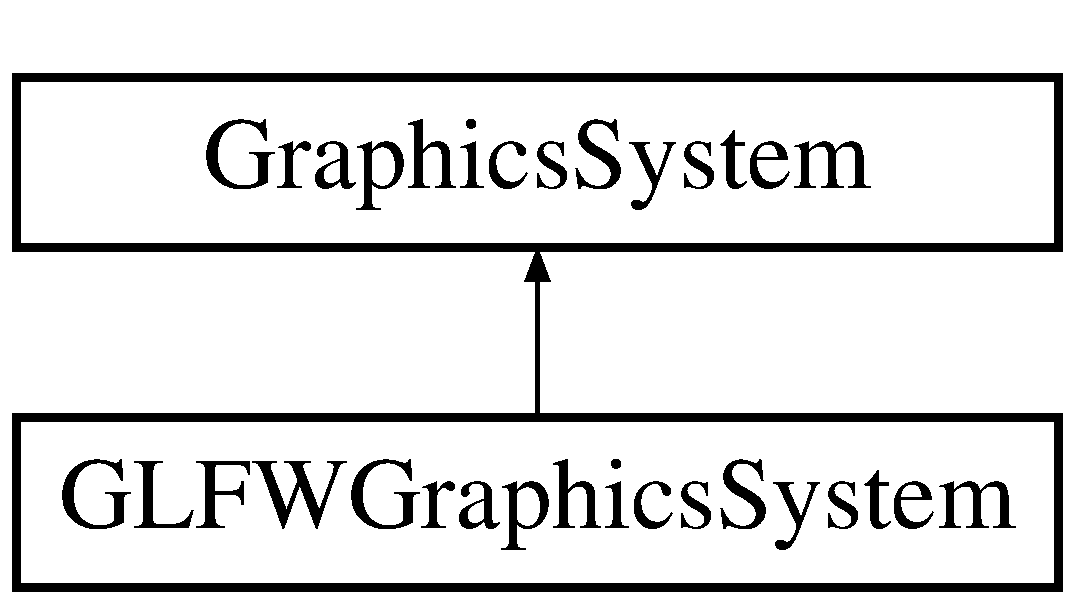
\includegraphics[height=2.000000cm]{class_graphics_system}
\end{center}
\end{figure}
\subsection*{Public Member Functions}
\begin{DoxyCompactItemize}
\item 
\hypertarget{class_graphics_system_a06c79c8ebe88092f8feff538f4082bd9}{}{\bfseries Graphics\+System} (\hyperlink{class_graphics_system}{Graphics\+System} const \&)\label{class_graphics_system_a06c79c8ebe88092f8feff538f4082bd9}

\item 
\hypertarget{class_graphics_system_a38d30a6bde4bf27c06ca814ed760e25b}{}void {\bfseries operator=} (\hyperlink{class_graphics_system}{Graphics\+System} const \&)\label{class_graphics_system_a38d30a6bde4bf27c06ca814ed760e25b}

\item 
virtual int \hyperlink{class_graphics_system_a7cdc16551f8da01c5271dfb64f807726}{init} (int width, int height)=0
\item 
virtual void \hyperlink{class_graphics_system_a00275fa0e3cc3b9274739b21d4ae9821}{shutdown} ()=0
\item 
virtual void \hyperlink{class_graphics_system_a24a513387448dac9db6510a01acfcaa6}{swap} ()=0
\item 
virtual void \hyperlink{class_graphics_system_acb34692fa9eb3c03c8a80ddfb6ea1e3f}{clear} ()=0
\item 
virtual void \hyperlink{class_graphics_system_a235c9266682e6521135003593409b92e}{create\+Debug\+Shader} ()=0
\item 
virtual int \hyperlink{class_graphics_system_a9ebe243b7671cf0a4486bb9ae1f458f9}{get\+Screen\+Width} ()=0
\item 
virtual int \hyperlink{class_graphics_system_a056ee98bac2643fabd540f0541707cce}{get\+Screen\+Height} ()=0
\item 
virtual void \hyperlink{class_graphics_system_a60e5c663c8b19a5fee37e40ef347e86e}{render} (shared\+\_\+ptr$<$ \hyperlink{class_camera}{Camera} $>$ camera, const physx\+::\+Px\+Render\+Buffer \&rb, const glm\+::vec4 \&color)=0
\item 
virtual void \hyperlink{class_graphics_system_a7fdefc85d986133bc43885f863cc9c7c}{render} (shared\+\_\+ptr$<$ \hyperlink{class_camera}{Camera} $>$ camera, vector$<$ shared\+\_\+ptr$<$ \hyperlink{class_mesh_renderer}{Mesh\+Renderer} $>$$>$ \&renderers, vector$<$ shared\+\_\+ptr$<$ \hyperlink{class_light}{Light} $>$$>$ \&lights)=0
\item 
virtual void \hyperlink{class_graphics_system_ac20abca82bc8163895b3f143eb53f113}{render\+G\+U\+I} (vector$<$ shared\+\_\+ptr$<$ U\+I\+Widget $>$$>$ ui\+Widget\+Vector)=0
\item 
virtual void \hyperlink{class_graphics_system_a32ab75f493e9037c83b718f5ccb11500}{generate\+Vertex\+Arrays} (const G\+Luint size, G\+Luint \&vao)=0
\item 
virtual void \hyperlink{class_graphics_system_a6ca91563b69a554462fccbcfff2d6a70}{generate\+Buffer} (const G\+Luint size, G\+Luint \&bo, G\+Lenum type, int data\+Size, void $\ast$data\+Pointer, G\+Lenum draw\+Type)=0
\item 
virtual void \hyperlink{class_graphics_system_a526e6b5fea898f4ac06ef0d0ab7b9d67}{delete\+Buffer} (G\+Luint size, G\+Luint \&bo)=0
\item 
virtual G\+Luint \hyperlink{class_graphics_system_a352afd81ae42f6415b4e28ff445e5d45}{create\+Shader} (G\+Lenum shader\+Type)=0
\item 
virtual void \hyperlink{class_graphics_system_ad287e692cbaab0fd5560df2f0cd98fc7}{compile\+Shader} (G\+Luint shader\+I\+D, G\+Luint size, const char $\ast$data\+Pointer)=0
\item 
virtual G\+Luint \hyperlink{class_graphics_system_a6c8d55818a976c504faf291c78f51ca5}{create\+Shader\+Program} ()=0
\item 
virtual void \hyperlink{class_graphics_system_aa166087f35ee2af8a9c9a45bd4a6103d}{attach\+And\+Link\+Shader} (G\+Luint Program\+I\+D, G\+Luint Vertex\+Shader\+I\+D, G\+Luint Fragment\+Shader\+I\+D)=0
\item 
virtual void \hyperlink{class_graphics_system_ab56e3749349d38b97fdb5fecd5a184e8}{delete\+Shader} (G\+Luint shader\+I\+D)=0
\item 
virtual G\+Lint \hyperlink{class_graphics_system_a32d2b6a92081eb59245849777f82f935}{get\+Uniform\+Location} (G\+Luint program\+I\+D, const char $\ast$name)=0
\item 
\hypertarget{class_graphics_system_a875158c6666076c397bd9406cfee079f}{}virtual shared\+\_\+ptr$<$ \hyperlink{class_texture}{Texture} $>$ {\bfseries get\+Default\+Texture} ()=0\label{class_graphics_system_a875158c6666076c397bd9406cfee079f}

\item 
virtual shared\+\_\+ptr$<$ G\+L\+F\+Wwindow $>$ \hyperlink{class_graphics_system_a0aeb3c0874bf9ca6ebc5ae5cb95bf859}{get\+Window} ()
\end{DoxyCompactItemize}
\subsection*{Static Public Member Functions}
\begin{DoxyCompactItemize}
\item 
\hypertarget{class_graphics_system_aa312ed8e67a459472cc90bf0e2c24b6d}{}static \hyperlink{class_graphics_system}{Graphics\+System} $\ast$ {\bfseries get\+Instance} ()\label{class_graphics_system_aa312ed8e67a459472cc90bf0e2c24b6d}

\end{DoxyCompactItemize}
\subsection*{Protected Attributes}
\begin{DoxyCompactItemize}
\item 
shared\+\_\+ptr$<$ G\+L\+F\+Wwindow $>$ \hyperlink{class_graphics_system_af64c8566c04ec068df5c50755b46e034}{window}
\item 
shared\+\_\+ptr$<$ \hyperlink{class_shader}{Shader} $>$ \hyperlink{class_graphics_system_a4598a940b017484e0c05f8b8d29eada0}{debug\+Shader}
\item 
shared\+\_\+ptr$<$ \hyperlink{class_material}{Material} $>$ \hyperlink{class_graphics_system_a0cc4e68c988b0181b4a72fe38931d4a1}{debug\+Material}
\item 
shared\+\_\+ptr$<$ \hyperlink{class_shader}{Shader} $>$ \hyperlink{class_graphics_system_aba28cabec543d87fa086bf64c41a7d1e}{gui\+Shader}
\item 
shared\+\_\+ptr$<$ \hyperlink{class_material}{Material} $>$ \hyperlink{class_graphics_system_afec79bbb5e358ea7f02ad7110017f333}{gui\+Material}
\item 
\hypertarget{class_graphics_system_ab3c54be1466226ad1fa45d8a68337f59}{}glm\+::mat4 {\bfseries G\+U\+I\+Matrix}\label{class_graphics_system_ab3c54be1466226ad1fa45d8a68337f59}

\end{DoxyCompactItemize}


\subsection{Detailed Description}
\hyperlink{class_graphics_system}{Graphics\+System} handles the Graphics of the Engine.

The idea behind creating an abstract class would be to allow for different Graphic A\+P\+I\textquotesingle{}s to handle how images are drawn. For example, change from Open\+G\+L to Direct\+X easily.

This is the class that knows how to draw images on the screen. 

\subsection{Member Function Documentation}
\hypertarget{class_graphics_system_aa166087f35ee2af8a9c9a45bd4a6103d}{}\index{Graphics\+System@{Graphics\+System}!attach\+And\+Link\+Shader@{attach\+And\+Link\+Shader}}
\index{attach\+And\+Link\+Shader@{attach\+And\+Link\+Shader}!Graphics\+System@{Graphics\+System}}
\subsubsection[{attach\+And\+Link\+Shader(\+G\+Luint Program\+I\+D, G\+Luint Vertex\+Shader\+I\+D, G\+Luint Fragment\+Shader\+I\+D)=0}]{\setlength{\rightskip}{0pt plus 5cm}virtual void Graphics\+System\+::attach\+And\+Link\+Shader (
\begin{DoxyParamCaption}
\item[{G\+Luint}]{Program\+I\+D, }
\item[{G\+Luint}]{Vertex\+Shader\+I\+D, }
\item[{G\+Luint}]{Fragment\+Shader\+I\+D}
\end{DoxyParamCaption}
)\hspace{0.3cm}{\ttfamily [pure virtual]}}\label{class_graphics_system_aa166087f35ee2af8a9c9a45bd4a6103d}
Merge Vertex\+Shader and Fragment\+Shader to one 

Implemented in \hyperlink{class_g_l_f_w_graphics_system_a1b993a6ed176405ba676d2f5569d373e}{G\+L\+F\+W\+Graphics\+System}.

\hypertarget{class_graphics_system_acb34692fa9eb3c03c8a80ddfb6ea1e3f}{}\index{Graphics\+System@{Graphics\+System}!clear@{clear}}
\index{clear@{clear}!Graphics\+System@{Graphics\+System}}
\subsubsection[{clear()=0}]{\setlength{\rightskip}{0pt plus 5cm}virtual void Graphics\+System\+::clear (
\begin{DoxyParamCaption}
{}
\end{DoxyParamCaption}
)\hspace{0.3cm}{\ttfamily [pure virtual]}}\label{class_graphics_system_acb34692fa9eb3c03c8a80ddfb6ea1e3f}
Clear buffers 

Implemented in \hyperlink{class_g_l_f_w_graphics_system_a84767a0209a04f598b866048e04b2035}{G\+L\+F\+W\+Graphics\+System}.

\hypertarget{class_graphics_system_ad287e692cbaab0fd5560df2f0cd98fc7}{}\index{Graphics\+System@{Graphics\+System}!compile\+Shader@{compile\+Shader}}
\index{compile\+Shader@{compile\+Shader}!Graphics\+System@{Graphics\+System}}
\subsubsection[{compile\+Shader(\+G\+Luint shader\+I\+D, G\+Luint size, const char $\ast$data\+Pointer)=0}]{\setlength{\rightskip}{0pt plus 5cm}virtual void Graphics\+System\+::compile\+Shader (
\begin{DoxyParamCaption}
\item[{G\+Luint}]{shader\+I\+D, }
\item[{G\+Luint}]{size, }
\item[{const char $\ast$}]{data\+Pointer}
\end{DoxyParamCaption}
)\hspace{0.3cm}{\ttfamily [pure virtual]}}\label{class_graphics_system_ad287e692cbaab0fd5560df2f0cd98fc7}
Compile the shader 

Implemented in \hyperlink{class_g_l_f_w_graphics_system_a87e2461accc1340e6ebc568729a8019a}{G\+L\+F\+W\+Graphics\+System}.

\hypertarget{class_graphics_system_a235c9266682e6521135003593409b92e}{}\index{Graphics\+System@{Graphics\+System}!create\+Debug\+Shader@{create\+Debug\+Shader}}
\index{create\+Debug\+Shader@{create\+Debug\+Shader}!Graphics\+System@{Graphics\+System}}
\subsubsection[{create\+Debug\+Shader()=0}]{\setlength{\rightskip}{0pt plus 5cm}virtual void Graphics\+System\+::create\+Debug\+Shader (
\begin{DoxyParamCaption}
{}
\end{DoxyParamCaption}
)\hspace{0.3cm}{\ttfamily [pure virtual]}}\label{class_graphics_system_a235c9266682e6521135003593409b92e}
create debug shader to display \hyperlink{class_physics}{Physics} information on the screen 

Implemented in \hyperlink{class_g_l_f_w_graphics_system_a446723c2cad999498d013f71ab8e570f}{G\+L\+F\+W\+Graphics\+System}.

\hypertarget{class_graphics_system_a352afd81ae42f6415b4e28ff445e5d45}{}\index{Graphics\+System@{Graphics\+System}!create\+Shader@{create\+Shader}}
\index{create\+Shader@{create\+Shader}!Graphics\+System@{Graphics\+System}}
\subsubsection[{create\+Shader(\+G\+Lenum shader\+Type)=0}]{\setlength{\rightskip}{0pt plus 5cm}virtual G\+Luint Graphics\+System\+::create\+Shader (
\begin{DoxyParamCaption}
\item[{G\+Lenum}]{shader\+Type}
\end{DoxyParamCaption}
)\hspace{0.3cm}{\ttfamily [pure virtual]}}\label{class_graphics_system_a352afd81ae42f6415b4e28ff445e5d45}
Creates a new shader 

Implemented in \hyperlink{class_g_l_f_w_graphics_system_a366ee287cdf55396fdd846e59235f2ea}{G\+L\+F\+W\+Graphics\+System}.

\hypertarget{class_graphics_system_a6c8d55818a976c504faf291c78f51ca5}{}\index{Graphics\+System@{Graphics\+System}!create\+Shader\+Program@{create\+Shader\+Program}}
\index{create\+Shader\+Program@{create\+Shader\+Program}!Graphics\+System@{Graphics\+System}}
\subsubsection[{create\+Shader\+Program()=0}]{\setlength{\rightskip}{0pt plus 5cm}virtual G\+Luint Graphics\+System\+::create\+Shader\+Program (
\begin{DoxyParamCaption}
{}
\end{DoxyParamCaption}
)\hspace{0.3cm}{\ttfamily [pure virtual]}}\label{class_graphics_system_a6c8d55818a976c504faf291c78f51ca5}
Creates a new shader program 

Implemented in \hyperlink{class_g_l_f_w_graphics_system_ac188b290e2647010d1ad8c0a07d63cf0}{G\+L\+F\+W\+Graphics\+System}.

\hypertarget{class_graphics_system_a526e6b5fea898f4ac06ef0d0ab7b9d67}{}\index{Graphics\+System@{Graphics\+System}!delete\+Buffer@{delete\+Buffer}}
\index{delete\+Buffer@{delete\+Buffer}!Graphics\+System@{Graphics\+System}}
\subsubsection[{delete\+Buffer(\+G\+Luint size, G\+Luint \&bo)=0}]{\setlength{\rightskip}{0pt plus 5cm}virtual void Graphics\+System\+::delete\+Buffer (
\begin{DoxyParamCaption}
\item[{G\+Luint}]{size, }
\item[{G\+Luint \&}]{bo}
\end{DoxyParamCaption}
)\hspace{0.3cm}{\ttfamily [pure virtual]}}\label{class_graphics_system_a526e6b5fea898f4ac06ef0d0ab7b9d67}
Release buffer 

Implemented in \hyperlink{class_g_l_f_w_graphics_system_aa7d78cc01b84a7ab6d90343d5adf4432}{G\+L\+F\+W\+Graphics\+System}.

\hypertarget{class_graphics_system_ab56e3749349d38b97fdb5fecd5a184e8}{}\index{Graphics\+System@{Graphics\+System}!delete\+Shader@{delete\+Shader}}
\index{delete\+Shader@{delete\+Shader}!Graphics\+System@{Graphics\+System}}
\subsubsection[{delete\+Shader(\+G\+Luint shader\+I\+D)=0}]{\setlength{\rightskip}{0pt plus 5cm}virtual void Graphics\+System\+::delete\+Shader (
\begin{DoxyParamCaption}
\item[{G\+Luint}]{shader\+I\+D}
\end{DoxyParamCaption}
)\hspace{0.3cm}{\ttfamily [pure virtual]}}\label{class_graphics_system_ab56e3749349d38b97fdb5fecd5a184e8}
Release shader 

Implemented in \hyperlink{class_g_l_f_w_graphics_system_a9a791ee2a7a5465cff955bc03451c998}{G\+L\+F\+W\+Graphics\+System}.

\hypertarget{class_graphics_system_a6ca91563b69a554462fccbcfff2d6a70}{}\index{Graphics\+System@{Graphics\+System}!generate\+Buffer@{generate\+Buffer}}
\index{generate\+Buffer@{generate\+Buffer}!Graphics\+System@{Graphics\+System}}
\subsubsection[{generate\+Buffer(const G\+Luint size, G\+Luint \&bo, G\+Lenum type, int data\+Size, void $\ast$data\+Pointer, G\+Lenum draw\+Type)=0}]{\setlength{\rightskip}{0pt plus 5cm}virtual void Graphics\+System\+::generate\+Buffer (
\begin{DoxyParamCaption}
\item[{const G\+Luint}]{size, }
\item[{G\+Luint \&}]{bo, }
\item[{G\+Lenum}]{type, }
\item[{int}]{data\+Size, }
\item[{void $\ast$}]{data\+Pointer, }
\item[{G\+Lenum}]{draw\+Type}
\end{DoxyParamCaption}
)\hspace{0.3cm}{\ttfamily [pure virtual]}}\label{class_graphics_system_a6ca91563b69a554462fccbcfff2d6a70}
Generates a new Buffer Array 

Implemented in \hyperlink{class_g_l_f_w_graphics_system_a22f72c31efab822c4d958a217f61340c}{G\+L\+F\+W\+Graphics\+System}.

\hypertarget{class_graphics_system_a32ab75f493e9037c83b718f5ccb11500}{}\index{Graphics\+System@{Graphics\+System}!generate\+Vertex\+Arrays@{generate\+Vertex\+Arrays}}
\index{generate\+Vertex\+Arrays@{generate\+Vertex\+Arrays}!Graphics\+System@{Graphics\+System}}
\subsubsection[{generate\+Vertex\+Arrays(const G\+Luint size, G\+Luint \&vao)=0}]{\setlength{\rightskip}{0pt plus 5cm}virtual void Graphics\+System\+::generate\+Vertex\+Arrays (
\begin{DoxyParamCaption}
\item[{const G\+Luint}]{size, }
\item[{G\+Luint \&}]{vao}
\end{DoxyParamCaption}
)\hspace{0.3cm}{\ttfamily [pure virtual]}}\label{class_graphics_system_a32ab75f493e9037c83b718f5ccb11500}
Generates a new Vertex Array -\/ Used for mesh vertice data 

Implemented in \hyperlink{class_g_l_f_w_graphics_system_a6b40d73f5eea98cebe77e51f7cba8f6c}{G\+L\+F\+W\+Graphics\+System}.

\hypertarget{class_graphics_system_a056ee98bac2643fabd540f0541707cce}{}\index{Graphics\+System@{Graphics\+System}!get\+Screen\+Height@{get\+Screen\+Height}}
\index{get\+Screen\+Height@{get\+Screen\+Height}!Graphics\+System@{Graphics\+System}}
\subsubsection[{get\+Screen\+Height()=0}]{\setlength{\rightskip}{0pt plus 5cm}virtual int Graphics\+System\+::get\+Screen\+Height (
\begin{DoxyParamCaption}
{}
\end{DoxyParamCaption}
)\hspace{0.3cm}{\ttfamily [pure virtual]}}\label{class_graphics_system_a056ee98bac2643fabd540f0541707cce}
screen height Getter 

Implemented in \hyperlink{class_g_l_f_w_graphics_system_ab6b0c31d3d5fb238a19c645630b87543}{G\+L\+F\+W\+Graphics\+System}.

\hypertarget{class_graphics_system_a9ebe243b7671cf0a4486bb9ae1f458f9}{}\index{Graphics\+System@{Graphics\+System}!get\+Screen\+Width@{get\+Screen\+Width}}
\index{get\+Screen\+Width@{get\+Screen\+Width}!Graphics\+System@{Graphics\+System}}
\subsubsection[{get\+Screen\+Width()=0}]{\setlength{\rightskip}{0pt plus 5cm}virtual int Graphics\+System\+::get\+Screen\+Width (
\begin{DoxyParamCaption}
{}
\end{DoxyParamCaption}
)\hspace{0.3cm}{\ttfamily [pure virtual]}}\label{class_graphics_system_a9ebe243b7671cf0a4486bb9ae1f458f9}
screen width Getter 

Implemented in \hyperlink{class_g_l_f_w_graphics_system_a8c31a0ea165e6c9cbd0e0c656342a200}{G\+L\+F\+W\+Graphics\+System}.

\hypertarget{class_graphics_system_a32d2b6a92081eb59245849777f82f935}{}\index{Graphics\+System@{Graphics\+System}!get\+Uniform\+Location@{get\+Uniform\+Location}}
\index{get\+Uniform\+Location@{get\+Uniform\+Location}!Graphics\+System@{Graphics\+System}}
\subsubsection[{get\+Uniform\+Location(\+G\+Luint program\+I\+D, const char $\ast$name)=0}]{\setlength{\rightskip}{0pt plus 5cm}virtual G\+Lint Graphics\+System\+::get\+Uniform\+Location (
\begin{DoxyParamCaption}
\item[{G\+Luint}]{program\+I\+D, }
\item[{const char $\ast$}]{name}
\end{DoxyParamCaption}
)\hspace{0.3cm}{\ttfamily [pure virtual]}}\label{class_graphics_system_a32d2b6a92081eb59245849777f82f935}
Gets the uniform location for a string in a shader 

Implemented in \hyperlink{class_g_l_f_w_graphics_system_ad7f9cc29bfe40cf3d498962fd50ccc16}{G\+L\+F\+W\+Graphics\+System}.

\hypertarget{class_graphics_system_a0aeb3c0874bf9ca6ebc5ae5cb95bf859}{}\index{Graphics\+System@{Graphics\+System}!get\+Window@{get\+Window}}
\index{get\+Window@{get\+Window}!Graphics\+System@{Graphics\+System}}
\subsubsection[{get\+Window()}]{\setlength{\rightskip}{0pt plus 5cm}virtual shared\+\_\+ptr$<$G\+L\+F\+Wwindow$>$ Graphics\+System\+::get\+Window (
\begin{DoxyParamCaption}
{}
\end{DoxyParamCaption}
)\hspace{0.3cm}{\ttfamily [inline]}, {\ttfamily [virtual]}}\label{class_graphics_system_a0aeb3c0874bf9ca6ebc5ae5cb95bf859}
window Getter \hypertarget{class_graphics_system_a7cdc16551f8da01c5271dfb64f807726}{}\index{Graphics\+System@{Graphics\+System}!init@{init}}
\index{init@{init}!Graphics\+System@{Graphics\+System}}
\subsubsection[{init(int width, int height)=0}]{\setlength{\rightskip}{0pt plus 5cm}virtual int Graphics\+System\+::init (
\begin{DoxyParamCaption}
\item[{int}]{width, }
\item[{int}]{height}
\end{DoxyParamCaption}
)\hspace{0.3cm}{\ttfamily [pure virtual]}}\label{class_graphics_system_a7cdc16551f8da01c5271dfb64f807726}
Initialize the system, create the window and such 

Implemented in \hyperlink{class_g_l_f_w_graphics_system_a4cba85b32cd751aab2f5a84c01199953}{G\+L\+F\+W\+Graphics\+System}.

\hypertarget{class_graphics_system_a60e5c663c8b19a5fee37e40ef347e86e}{}\index{Graphics\+System@{Graphics\+System}!render@{render}}
\index{render@{render}!Graphics\+System@{Graphics\+System}}
\subsubsection[{render(shared\+\_\+ptr$<$ Camera $>$ camera, const physx\+::\+Px\+Render\+Buffer \&rb, const glm\+::vec4 \&color)=0}]{\setlength{\rightskip}{0pt plus 5cm}virtual void Graphics\+System\+::render (
\begin{DoxyParamCaption}
\item[{shared\+\_\+ptr$<$ {\bf Camera} $>$}]{camera, }
\item[{const physx\+::\+Px\+Render\+Buffer \&}]{rb, }
\item[{const glm\+::vec4 \&}]{color}
\end{DoxyParamCaption}
)\hspace{0.3cm}{\ttfamily [pure virtual]}}\label{class_graphics_system_a60e5c663c8b19a5fee37e40ef347e86e}
Renders \hyperlink{class_physics}{Physics} information on screen from the camera point of view 

Implemented in \hyperlink{class_g_l_f_w_graphics_system_a606c4e6e8e53084d3d23bc7bbcdfc228}{G\+L\+F\+W\+Graphics\+System}.

\hypertarget{class_graphics_system_a7fdefc85d986133bc43885f863cc9c7c}{}\index{Graphics\+System@{Graphics\+System}!render@{render}}
\index{render@{render}!Graphics\+System@{Graphics\+System}}
\subsubsection[{render(shared\+\_\+ptr$<$ Camera $>$ camera, vector$<$ shared\+\_\+ptr$<$ Mesh\+Renderer $>$$>$ \&renderers, vector$<$ shared\+\_\+ptr$<$ Light $>$$>$ \&lights)=0}]{\setlength{\rightskip}{0pt plus 5cm}virtual void Graphics\+System\+::render (
\begin{DoxyParamCaption}
\item[{shared\+\_\+ptr$<$ {\bf Camera} $>$}]{camera, }
\item[{vector$<$ shared\+\_\+ptr$<$ {\bf Mesh\+Renderer} $>$$>$ \&}]{renderers, }
\item[{vector$<$ shared\+\_\+ptr$<$ {\bf Light} $>$$>$ \&}]{lights}
\end{DoxyParamCaption}
)\hspace{0.3cm}{\ttfamily [pure virtual]}}\label{class_graphics_system_a7fdefc85d986133bc43885f863cc9c7c}
Renders meshes on the screen from the camera point of view 

Implemented in \hyperlink{class_g_l_f_w_graphics_system_a2cde625e8606c2905d7728f2cadf7371}{G\+L\+F\+W\+Graphics\+System}.

\hypertarget{class_graphics_system_ac20abca82bc8163895b3f143eb53f113}{}\index{Graphics\+System@{Graphics\+System}!render\+G\+U\+I@{render\+G\+U\+I}}
\index{render\+G\+U\+I@{render\+G\+U\+I}!Graphics\+System@{Graphics\+System}}
\subsubsection[{render\+G\+U\+I(vector$<$ shared\+\_\+ptr$<$ U\+I\+Widget $>$$>$ ui\+Widget\+Vector)=0}]{\setlength{\rightskip}{0pt plus 5cm}virtual void Graphics\+System\+::render\+G\+U\+I (
\begin{DoxyParamCaption}
\item[{vector$<$ shared\+\_\+ptr$<$ U\+I\+Widget $>$$>$}]{ui\+Widget\+Vector}
\end{DoxyParamCaption}
)\hspace{0.3cm}{\ttfamily [pure virtual]}}\label{class_graphics_system_ac20abca82bc8163895b3f143eb53f113}
Render Widgets on screen 

Implemented in \hyperlink{class_g_l_f_w_graphics_system_a8ebfaa6c98ba4a92618835de8966e8b9}{G\+L\+F\+W\+Graphics\+System}.

\hypertarget{class_graphics_system_a00275fa0e3cc3b9274739b21d4ae9821}{}\index{Graphics\+System@{Graphics\+System}!shutdown@{shutdown}}
\index{shutdown@{shutdown}!Graphics\+System@{Graphics\+System}}
\subsubsection[{shutdown()=0}]{\setlength{\rightskip}{0pt plus 5cm}virtual void Graphics\+System\+::shutdown (
\begin{DoxyParamCaption}
{}
\end{DoxyParamCaption}
)\hspace{0.3cm}{\ttfamily [pure virtual]}}\label{class_graphics_system_a00275fa0e3cc3b9274739b21d4ae9821}
Shutdown the system, destroy window and release any allocated memory 

Implemented in \hyperlink{class_g_l_f_w_graphics_system_ab12358c2a7034dcf75df074fbe4d86d4}{G\+L\+F\+W\+Graphics\+System}.

\hypertarget{class_graphics_system_a24a513387448dac9db6510a01acfcaa6}{}\index{Graphics\+System@{Graphics\+System}!swap@{swap}}
\index{swap@{swap}!Graphics\+System@{Graphics\+System}}
\subsubsection[{swap()=0}]{\setlength{\rightskip}{0pt plus 5cm}virtual void Graphics\+System\+::swap (
\begin{DoxyParamCaption}
{}
\end{DoxyParamCaption}
)\hspace{0.3cm}{\ttfamily [pure virtual]}}\label{class_graphics_system_a24a513387448dac9db6510a01acfcaa6}
Swap buffers 

Implemented in \hyperlink{class_g_l_f_w_graphics_system_a52ef8cd44b2b45828452626d9e0b54d6}{G\+L\+F\+W\+Graphics\+System}.



\subsection{Member Data Documentation}
\hypertarget{class_graphics_system_a0cc4e68c988b0181b4a72fe38931d4a1}{}\index{Graphics\+System@{Graphics\+System}!debug\+Material@{debug\+Material}}
\index{debug\+Material@{debug\+Material}!Graphics\+System@{Graphics\+System}}
\subsubsection[{debug\+Material}]{\setlength{\rightskip}{0pt plus 5cm}shared\+\_\+ptr$<${\bf Material}$>$ Graphics\+System\+::debug\+Material\hspace{0.3cm}{\ttfamily [protected]}}\label{class_graphics_system_a0cc4e68c988b0181b4a72fe38931d4a1}
\hyperlink{class_material}{Material} used to debug \hyperlink{class_physics}{Physics} Information \hypertarget{class_graphics_system_a4598a940b017484e0c05f8b8d29eada0}{}\index{Graphics\+System@{Graphics\+System}!debug\+Shader@{debug\+Shader}}
\index{debug\+Shader@{debug\+Shader}!Graphics\+System@{Graphics\+System}}
\subsubsection[{debug\+Shader}]{\setlength{\rightskip}{0pt plus 5cm}shared\+\_\+ptr$<${\bf Shader}$>$ Graphics\+System\+::debug\+Shader\hspace{0.3cm}{\ttfamily [protected]}}\label{class_graphics_system_a4598a940b017484e0c05f8b8d29eada0}
\hyperlink{class_shader}{Shader} used to debug \hyperlink{class_physics}{Physics} Information \hypertarget{class_graphics_system_afec79bbb5e358ea7f02ad7110017f333}{}\index{Graphics\+System@{Graphics\+System}!gui\+Material@{gui\+Material}}
\index{gui\+Material@{gui\+Material}!Graphics\+System@{Graphics\+System}}
\subsubsection[{gui\+Material}]{\setlength{\rightskip}{0pt plus 5cm}shared\+\_\+ptr$<${\bf Material}$>$ Graphics\+System\+::gui\+Material\hspace{0.3cm}{\ttfamily [protected]}}\label{class_graphics_system_afec79bbb5e358ea7f02ad7110017f333}
\hyperlink{class_material}{Material} used to render G\+U\+I \hypertarget{class_graphics_system_aba28cabec543d87fa086bf64c41a7d1e}{}\index{Graphics\+System@{Graphics\+System}!gui\+Shader@{gui\+Shader}}
\index{gui\+Shader@{gui\+Shader}!Graphics\+System@{Graphics\+System}}
\subsubsection[{gui\+Shader}]{\setlength{\rightskip}{0pt plus 5cm}shared\+\_\+ptr$<${\bf Shader}$>$ Graphics\+System\+::gui\+Shader\hspace{0.3cm}{\ttfamily [protected]}}\label{class_graphics_system_aba28cabec543d87fa086bf64c41a7d1e}
\hyperlink{class_shader}{Shader} used to render G\+U\+I \hypertarget{class_graphics_system_af64c8566c04ec068df5c50755b46e034}{}\index{Graphics\+System@{Graphics\+System}!window@{window}}
\index{window@{window}!Graphics\+System@{Graphics\+System}}
\subsubsection[{window}]{\setlength{\rightskip}{0pt plus 5cm}shared\+\_\+ptr$<$G\+L\+F\+Wwindow$>$ Graphics\+System\+::window\hspace{0.3cm}{\ttfamily [protected]}}\label{class_graphics_system_af64c8566c04ec068df5c50755b46e034}
Handle to the window 

The documentation for this class was generated from the following files\+:\begin{DoxyCompactItemize}
\item 
/\+Users/guilherme\+\_\+cunha/\+Dev/\+G\+I\+T\+H\+U\+B/\+G\+U\+Inity/\+Source/Graphics\+System.\+hpp\item 
/\+Users/guilherme\+\_\+cunha/\+Dev/\+G\+I\+T\+H\+U\+B/\+G\+U\+Inity/\+Source/Graphics\+System.\+cpp\end{DoxyCompactItemize}

\hypertarget{class_holder}{}\section{Holder Class Reference}
\label{class_holder}\index{Holder@{Holder}}


{\ttfamily \#include $<$Holder.\+hpp$>$}

\subsection*{Public Member Functions}
\begin{DoxyCompactItemize}
\item 
\hyperlink{class_holder_ae1dbc8fe3c2767fc8151053f12d92153}{Holder} (Shader\+Param\+Type type, float val)
\item 
\hyperlink{class_holder_ac3b91f721b1215045a8844646475a6c6}{Holder} (Shader\+Param\+Type type, const glm\+::vec4 \&val)
\item 
\hyperlink{class_holder_a380c68c69ef301e3af33c0aca9a48e98}{Holder} (Shader\+Param\+Type type, shared\+\_\+ptr$<$ \hyperlink{class_texture}{Texture} $>$ val)
\item 
bool \hyperlink{class_holder_a2cd1439c60fb135001774ab4e655c43a}{is\+Float} () const 
\item 
bool \hyperlink{class_holder_a9d261d1a676d922c3b859e5fd67e8a22}{is\+Vec4} () const 
\item 
bool \hyperlink{class_holder_adec8ccaac7d8750aca659c7264ec32ac}{is\+Texture} () const 
\item 
float \hyperlink{class_holder_ad8c5e5b50c6a726f77343c339d5fd706}{get\+Float} () const 
\item 
glm\+::vec4 \hyperlink{class_holder_a66a04f0ba3f38c073afebc8154920d63}{get\+Vec4} () const 
\item 
shared\+\_\+ptr$<$ \hyperlink{class_texture}{Texture} $>$ \hyperlink{class_holder_a41425780f640866a40c069b298d3532d}{get\+Texture} () const 
\end{DoxyCompactItemize}


\subsection{Detailed Description}
\hyperlink{class_holder}{Holder} is a class that can hold multiple values. It\textquotesingle{}s used by Materials and Shaders because each shader can contain several input parameters such as float values and Textures. 

\subsection{Constructor \& Destructor Documentation}
\hypertarget{class_holder_ae1dbc8fe3c2767fc8151053f12d92153}{}\index{Holder@{Holder}!Holder@{Holder}}
\index{Holder@{Holder}!Holder@{Holder}}
\subsubsection[{Holder(\+Shader\+Param\+Type type, float val)}]{\setlength{\rightskip}{0pt plus 5cm}Holder\+::\+Holder (
\begin{DoxyParamCaption}
\item[{Shader\+Param\+Type}]{type, }
\item[{float}]{val}
\end{DoxyParamCaption}
)\hspace{0.3cm}{\ttfamily [explicit]}}\label{class_holder_ae1dbc8fe3c2767fc8151053f12d92153}
The explicit is very important here because we don\textquotesingle{}t want any implicit conversions among types Constructor for a float

Constructor for a float \hypertarget{class_holder_ac3b91f721b1215045a8844646475a6c6}{}\index{Holder@{Holder}!Holder@{Holder}}
\index{Holder@{Holder}!Holder@{Holder}}
\subsubsection[{Holder(\+Shader\+Param\+Type type, const glm\+::vec4 \&val)}]{\setlength{\rightskip}{0pt plus 5cm}Holder\+::\+Holder (
\begin{DoxyParamCaption}
\item[{Shader\+Param\+Type}]{type, }
\item[{const glm\+::vec4 \&}]{val}
\end{DoxyParamCaption}
)\hspace{0.3cm}{\ttfamily [explicit]}}\label{class_holder_ac3b91f721b1215045a8844646475a6c6}
Constructor for a vec4 \hypertarget{class_holder_a380c68c69ef301e3af33c0aca9a48e98}{}\index{Holder@{Holder}!Holder@{Holder}}
\index{Holder@{Holder}!Holder@{Holder}}
\subsubsection[{Holder(\+Shader\+Param\+Type type, shared\+\_\+ptr$<$ Texture $>$ val)}]{\setlength{\rightskip}{0pt plus 5cm}Holder\+::\+Holder (
\begin{DoxyParamCaption}
\item[{Shader\+Param\+Type}]{type, }
\item[{shared\+\_\+ptr$<$ {\bf Texture} $>$}]{val}
\end{DoxyParamCaption}
)\hspace{0.3cm}{\ttfamily [explicit]}}\label{class_holder_a380c68c69ef301e3af33c0aca9a48e98}
Constructor for a \hyperlink{class_texture}{Texture} 

\subsection{Member Function Documentation}
\hypertarget{class_holder_ad8c5e5b50c6a726f77343c339d5fd706}{}\index{Holder@{Holder}!get\+Float@{get\+Float}}
\index{get\+Float@{get\+Float}!Holder@{Holder}}
\subsubsection[{get\+Float() const }]{\setlength{\rightskip}{0pt plus 5cm}float Holder\+::get\+Float (
\begin{DoxyParamCaption}
{}
\end{DoxyParamCaption}
) const}\label{class_holder_ad8c5e5b50c6a726f77343c339d5fd706}
returns the float value \hypertarget{class_holder_a41425780f640866a40c069b298d3532d}{}\index{Holder@{Holder}!get\+Texture@{get\+Texture}}
\index{get\+Texture@{get\+Texture}!Holder@{Holder}}
\subsubsection[{get\+Texture() const }]{\setlength{\rightskip}{0pt plus 5cm}shared\+\_\+ptr$<$ {\bf Texture} $>$ Holder\+::get\+Texture (
\begin{DoxyParamCaption}
{}
\end{DoxyParamCaption}
) const}\label{class_holder_a41425780f640866a40c069b298d3532d}
returns the \hyperlink{class_texture}{Texture} value \hypertarget{class_holder_a66a04f0ba3f38c073afebc8154920d63}{}\index{Holder@{Holder}!get\+Vec4@{get\+Vec4}}
\index{get\+Vec4@{get\+Vec4}!Holder@{Holder}}
\subsubsection[{get\+Vec4() const }]{\setlength{\rightskip}{0pt plus 5cm}glm\+::vec4 Holder\+::get\+Vec4 (
\begin{DoxyParamCaption}
{}
\end{DoxyParamCaption}
) const}\label{class_holder_a66a04f0ba3f38c073afebc8154920d63}
returns the vec4 value

returns the vec3 value \hypertarget{class_holder_a2cd1439c60fb135001774ab4e655c43a}{}\index{Holder@{Holder}!is\+Float@{is\+Float}}
\index{is\+Float@{is\+Float}!Holder@{Holder}}
\subsubsection[{is\+Float() const }]{\setlength{\rightskip}{0pt plus 5cm}bool Holder\+::is\+Float (
\begin{DoxyParamCaption}
{}
\end{DoxyParamCaption}
) const}\label{class_holder_a2cd1439c60fb135001774ab4e655c43a}
returns true if it is a float value \hypertarget{class_holder_adec8ccaac7d8750aca659c7264ec32ac}{}\index{Holder@{Holder}!is\+Texture@{is\+Texture}}
\index{is\+Texture@{is\+Texture}!Holder@{Holder}}
\subsubsection[{is\+Texture() const }]{\setlength{\rightskip}{0pt plus 5cm}bool Holder\+::is\+Texture (
\begin{DoxyParamCaption}
{}
\end{DoxyParamCaption}
) const}\label{class_holder_adec8ccaac7d8750aca659c7264ec32ac}
returns true if it is a \hyperlink{class_texture}{Texture} value \hypertarget{class_holder_a9d261d1a676d922c3b859e5fd67e8a22}{}\index{Holder@{Holder}!is\+Vec4@{is\+Vec4}}
\index{is\+Vec4@{is\+Vec4}!Holder@{Holder}}
\subsubsection[{is\+Vec4() const }]{\setlength{\rightskip}{0pt plus 5cm}bool Holder\+::is\+Vec4 (
\begin{DoxyParamCaption}
{}
\end{DoxyParamCaption}
) const}\label{class_holder_a9d261d1a676d922c3b859e5fd67e8a22}
returns true if it is a vec4 value

returns true if it is a vec3 value 

The documentation for this class was generated from the following files\+:\begin{DoxyCompactItemize}
\item 
/\+Users/guilherme\+\_\+cunha/\+Dev/\+G\+I\+T\+H\+U\+B/\+G\+U\+Inity/\+Source/Holder.\+hpp\item 
/\+Users/guilherme\+\_\+cunha/\+Dev/\+G\+I\+T\+H\+U\+B/\+G\+U\+Inity/\+Source/Holder.\+cpp\end{DoxyCompactItemize}

\hypertarget{class_increase_collider_script}{}\section{Increase\+Collider\+Script Class Reference}
\label{class_increase_collider_script}\index{Increase\+Collider\+Script@{Increase\+Collider\+Script}}
Inheritance diagram for Increase\+Collider\+Script\+:\begin{figure}[H]
\begin{center}
\leavevmode
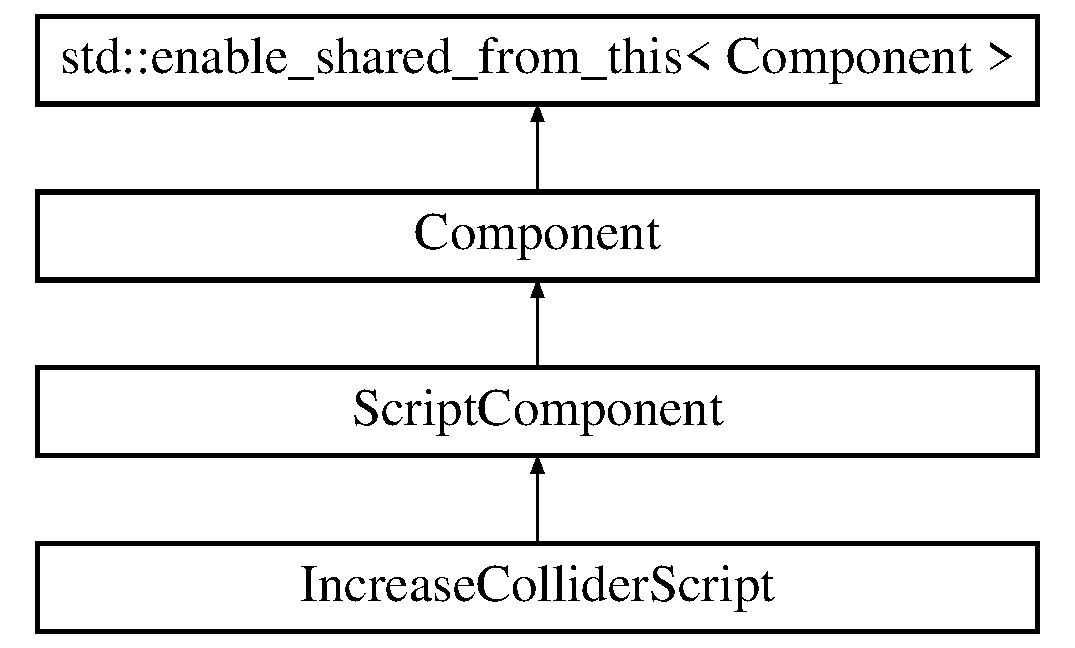
\includegraphics[height=4.000000cm]{class_increase_collider_script}
\end{center}
\end{figure}
\subsection*{Public Member Functions}
\begin{DoxyCompactItemize}
\item 
virtual void \hyperlink{class_increase_collider_script_a2a3291f10ec9cd908a0c45992847d7fe}{awake} () override
\item 
virtual void \hyperlink{class_increase_collider_script_a7be665f5544316bfd2ad39c32e66b11f}{tick} (float delta\+Secods) override
\end{DoxyCompactItemize}
\subsection*{Additional Inherited Members}


\subsection{Member Function Documentation}
\hypertarget{class_increase_collider_script_a2a3291f10ec9cd908a0c45992847d7fe}{}\index{Increase\+Collider\+Script@{Increase\+Collider\+Script}!awake@{awake}}
\index{awake@{awake}!Increase\+Collider\+Script@{Increase\+Collider\+Script}}
\subsubsection[{awake() override}]{\setlength{\rightskip}{0pt plus 5cm}void Increase\+Collider\+Script\+::awake (
\begin{DoxyParamCaption}
{}
\end{DoxyParamCaption}
)\hspace{0.3cm}{\ttfamily [override]}, {\ttfamily [virtual]}}\label{class_increase_collider_script_a2a3291f10ec9cd908a0c45992847d7fe}
\hyperlink{class_component}{Component} awake override 

Reimplemented from \hyperlink{class_script_component_a4667b8a3712e18b25cd6f49f12c5677d}{Script\+Component}.

\hypertarget{class_increase_collider_script_a7be665f5544316bfd2ad39c32e66b11f}{}\index{Increase\+Collider\+Script@{Increase\+Collider\+Script}!tick@{tick}}
\index{tick@{tick}!Increase\+Collider\+Script@{Increase\+Collider\+Script}}
\subsubsection[{tick(float delta\+Secods) override}]{\setlength{\rightskip}{0pt plus 5cm}void Increase\+Collider\+Script\+::tick (
\begin{DoxyParamCaption}
\item[{float}]{delta\+Secods}
\end{DoxyParamCaption}
)\hspace{0.3cm}{\ttfamily [override]}, {\ttfamily [virtual]}}\label{class_increase_collider_script_a7be665f5544316bfd2ad39c32e66b11f}
\hyperlink{class_component}{Component} tick override 
\begin{DoxyParams}[1]{Parameters}
\mbox{\tt in}  & {\em delta\+Seconds} & last frame durations \\
\hline
\end{DoxyParams}


Reimplemented from \hyperlink{class_script_component_aa765fa62a343a8d83eb168d369b93a51}{Script\+Component}.



The documentation for this class was generated from the following files\+:\begin{DoxyCompactItemize}
\item 
/\+Users/guilherme\+\_\+cunha/\+Dev/\+G\+I\+T\+H\+U\+B/\+G\+U\+Inity/\+Source/Increase\+Collider\+Script.\+hpp\item 
/\+Users/guilherme\+\_\+cunha/\+Dev/\+G\+I\+T\+H\+U\+B/\+G\+U\+Inity/\+Source/Increase\+Collider\+Script.\+cpp\end{DoxyCompactItemize}

\hypertarget{class_input}{}\section{Input Class Reference}
\label{class_input}\index{Input@{Input}}
\subsection*{Public Member Functions}
\begin{DoxyCompactItemize}
\item 
\hyperlink{class_input_a4bb10af47f86a631e374d4a5d01366b4}{Input} (shared\+\_\+ptr$<$ G\+L\+F\+Wwindow $>$ w)
\item 
\hyperlink{class_input_af2db35ba67c8a8ccd23bef6a482fc291}{$\sim$\+Input} ()
\end{DoxyCompactItemize}
\subsection*{Static Public Member Functions}
\begin{DoxyCompactItemize}
\item 
static bool \hyperlink{class_input_ab424be0c858611fbd1b36f7caf80f508}{get\+Key\+Pressed} (int key\+Code)
\item 
static bool \hyperlink{class_input_a4e14edb60b254707ca85b8d1b3f1e11c}{get\+Key\+Released} (int key\+Code)
\item 
static bool \hyperlink{class_input_a60956e1f7f561d18ac47bb192d669b67}{get\+Key} (int key\+Code)
\item 
static bool \hyperlink{class_input_aecdf0f7a65f5a57d55083673a437fce6}{get\+Mouse\+Button\+Pressed} (int key\+Code)
\item 
static bool \hyperlink{class_input_a00cede6f344f2c2594428fb51534f200}{get\+Mouse\+Button\+Released} (int key\+Code)
\item 
static bool \hyperlink{class_input_a18f4658d9875dd010fad6ba27c79e6db}{get\+Mouse\+Button} (int key\+Code)
\item 
static void \hyperlink{class_input_a7a7a5adb33a1570559f5cbe173eab4c2}{update\+Input\+State} ()
\item 
static shared\+\_\+ptr$<$ G\+L\+F\+Wwindow $>$ \hyperlink{class_input_ae778fda97d821417705d50d584c9a885}{get\+Window} ()
\item 
static void \hyperlink{class_input_a713c105c3e6479947f12c018d1dec7be}{set\+Window} (shared\+\_\+ptr$<$ G\+L\+F\+Wwindow $>$ window)
\end{DoxyCompactItemize}
\subsection*{Static Public Attributes}
\begin{DoxyCompactItemize}
\item 
static std\+::array$<$ int, n\+Keys $>$ \hyperlink{class_input_ad6f01906250d4f81f5d75ec3adfef210}{old\+Keyboard\+Input\+State} = \{ 0 \}
\item 
static std\+::array$<$ int, n\+Keys $>$ \hyperlink{class_input_a97eec171d280642b3a52c296503c2664}{keyboard\+Input\+State} = \{ 0 \}
\item 
static std\+::array$<$ int, n\+Mouse\+Buttons $>$ \hyperlink{class_input_a3b5a18a878d9c36cf3f27b30cfb1fce4}{old\+Mouse\+Input\+State} = \{ 0 \}
\item 
static std\+::array$<$ int, n\+Mouse\+Buttons $>$ \hyperlink{class_input_afd2b6ea6a62a21bb5af4d5d7688b9509}{mouse\+Input\+State} = \{ 0 \}
\item 
static glm\+::vec2 \hyperlink{class_input_a43c2217c224a48ff3af89ee9e284df69}{last\+Mouse\+Pos}
\item 
static glm\+::vec2 \hyperlink{class_input_a8a4e33aea3c586f5f327c51aed20e33e}{mouse\+Pos}
\item 
static glm\+::vec2 \hyperlink{class_input_ab86bb9716a4ac0ca353eade82c20cf7f}{mouse\+Delta}
\end{DoxyCompactItemize}


\subsection{Constructor \& Destructor Documentation}
\hypertarget{class_input_a4bb10af47f86a631e374d4a5d01366b4}{}\index{Input@{Input}!Input@{Input}}
\index{Input@{Input}!Input@{Input}}
\subsubsection[{Input(shared\+\_\+ptr$<$ G\+L\+F\+Wwindow $>$ w)}]{\setlength{\rightskip}{0pt plus 5cm}Input\+::\+Input (
\begin{DoxyParamCaption}
\item[{shared\+\_\+ptr$<$ G\+L\+F\+Wwindow $>$}]{w}
\end{DoxyParamCaption}
)}\label{class_input_a4bb10af47f86a631e374d4a5d01366b4}
Constructor for a window handle \hypertarget{class_input_af2db35ba67c8a8ccd23bef6a482fc291}{}\index{Input@{Input}!````~Input@{$\sim$\+Input}}
\index{````~Input@{$\sim$\+Input}!Input@{Input}}
\subsubsection[{$\sim$\+Input()}]{\setlength{\rightskip}{0pt plus 5cm}Input\+::$\sim$\+Input (
\begin{DoxyParamCaption}
{}
\end{DoxyParamCaption}
)\hspace{0.3cm}{\ttfamily [inline]}}\label{class_input_af2db35ba67c8a8ccd23bef6a482fc291}
Default destructor 

\subsection{Member Function Documentation}
\hypertarget{class_input_a60956e1f7f561d18ac47bb192d669b67}{}\index{Input@{Input}!get\+Key@{get\+Key}}
\index{get\+Key@{get\+Key}!Input@{Input}}
\subsubsection[{get\+Key(int key\+Code)}]{\setlength{\rightskip}{0pt plus 5cm}bool Input\+::get\+Key (
\begin{DoxyParamCaption}
\item[{int}]{key\+Code}
\end{DoxyParamCaption}
)\hspace{0.3cm}{\ttfamily [static]}}\label{class_input_a60956e1f7f561d18ac47bb192d669b67}
Returns true if the key I\+S pressed (every frame that the key is pressed) \hypertarget{class_input_ab424be0c858611fbd1b36f7caf80f508}{}\index{Input@{Input}!get\+Key\+Pressed@{get\+Key\+Pressed}}
\index{get\+Key\+Pressed@{get\+Key\+Pressed}!Input@{Input}}
\subsubsection[{get\+Key\+Pressed(int key\+Code)}]{\setlength{\rightskip}{0pt plus 5cm}bool Input\+::get\+Key\+Pressed (
\begin{DoxyParamCaption}
\item[{int}]{key\+Code}
\end{DoxyParamCaption}
)\hspace{0.3cm}{\ttfamily [static]}}\label{class_input_ab424be0c858611fbd1b36f7caf80f508}
Returns true if the key was pressed (1st frame only) \hypertarget{class_input_a4e14edb60b254707ca85b8d1b3f1e11c}{}\index{Input@{Input}!get\+Key\+Released@{get\+Key\+Released}}
\index{get\+Key\+Released@{get\+Key\+Released}!Input@{Input}}
\subsubsection[{get\+Key\+Released(int key\+Code)}]{\setlength{\rightskip}{0pt plus 5cm}bool Input\+::get\+Key\+Released (
\begin{DoxyParamCaption}
\item[{int}]{key\+Code}
\end{DoxyParamCaption}
)\hspace{0.3cm}{\ttfamily [static]}}\label{class_input_a4e14edb60b254707ca85b8d1b3f1e11c}
Returns true if the key was pressed (release frame only) \hypertarget{class_input_a18f4658d9875dd010fad6ba27c79e6db}{}\index{Input@{Input}!get\+Mouse\+Button@{get\+Mouse\+Button}}
\index{get\+Mouse\+Button@{get\+Mouse\+Button}!Input@{Input}}
\subsubsection[{get\+Mouse\+Button(int key\+Code)}]{\setlength{\rightskip}{0pt plus 5cm}bool Input\+::get\+Mouse\+Button (
\begin{DoxyParamCaption}
\item[{int}]{key\+Code}
\end{DoxyParamCaption}
)\hspace{0.3cm}{\ttfamily [static]}}\label{class_input_a18f4658d9875dd010fad6ba27c79e6db}
Returns true if the mouse button I\+S pressed (every frame that the mouse button is pressed) \hypertarget{class_input_aecdf0f7a65f5a57d55083673a437fce6}{}\index{Input@{Input}!get\+Mouse\+Button\+Pressed@{get\+Mouse\+Button\+Pressed}}
\index{get\+Mouse\+Button\+Pressed@{get\+Mouse\+Button\+Pressed}!Input@{Input}}
\subsubsection[{get\+Mouse\+Button\+Pressed(int key\+Code)}]{\setlength{\rightskip}{0pt plus 5cm}bool Input\+::get\+Mouse\+Button\+Pressed (
\begin{DoxyParamCaption}
\item[{int}]{key\+Code}
\end{DoxyParamCaption}
)\hspace{0.3cm}{\ttfamily [static]}}\label{class_input_aecdf0f7a65f5a57d55083673a437fce6}
Returns true if the mouse button was pressed (1st frame only) \hypertarget{class_input_a00cede6f344f2c2594428fb51534f200}{}\index{Input@{Input}!get\+Mouse\+Button\+Released@{get\+Mouse\+Button\+Released}}
\index{get\+Mouse\+Button\+Released@{get\+Mouse\+Button\+Released}!Input@{Input}}
\subsubsection[{get\+Mouse\+Button\+Released(int key\+Code)}]{\setlength{\rightskip}{0pt plus 5cm}bool Input\+::get\+Mouse\+Button\+Released (
\begin{DoxyParamCaption}
\item[{int}]{key\+Code}
\end{DoxyParamCaption}
)\hspace{0.3cm}{\ttfamily [static]}}\label{class_input_a00cede6f344f2c2594428fb51534f200}
Returns true if the mouse button was pressed (release frame only) \hypertarget{class_input_ae778fda97d821417705d50d584c9a885}{}\index{Input@{Input}!get\+Window@{get\+Window}}
\index{get\+Window@{get\+Window}!Input@{Input}}
\subsubsection[{get\+Window()}]{\setlength{\rightskip}{0pt plus 5cm}static shared\+\_\+ptr$<$G\+L\+F\+Wwindow$>$ Input\+::get\+Window (
\begin{DoxyParamCaption}
{}
\end{DoxyParamCaption}
)\hspace{0.3cm}{\ttfamily [static]}}\label{class_input_ae778fda97d821417705d50d584c9a885}
window getter \hypertarget{class_input_a713c105c3e6479947f12c018d1dec7be}{}\index{Input@{Input}!set\+Window@{set\+Window}}
\index{set\+Window@{set\+Window}!Input@{Input}}
\subsubsection[{set\+Window(shared\+\_\+ptr$<$ G\+L\+F\+Wwindow $>$ window)}]{\setlength{\rightskip}{0pt plus 5cm}static void Input\+::set\+Window (
\begin{DoxyParamCaption}
\item[{shared\+\_\+ptr$<$ G\+L\+F\+Wwindow $>$}]{window}
\end{DoxyParamCaption}
)\hspace{0.3cm}{\ttfamily [static]}}\label{class_input_a713c105c3e6479947f12c018d1dec7be}
window setter \hypertarget{class_input_a7a7a5adb33a1570559f5cbe173eab4c2}{}\index{Input@{Input}!update\+Input\+State@{update\+Input\+State}}
\index{update\+Input\+State@{update\+Input\+State}!Input@{Input}}
\subsubsection[{update\+Input\+State()}]{\setlength{\rightskip}{0pt plus 5cm}void Input\+::update\+Input\+State (
\begin{DoxyParamCaption}
{}
\end{DoxyParamCaption}
)\hspace{0.3cm}{\ttfamily [static]}}\label{class_input_a7a7a5adb33a1570559f5cbe173eab4c2}
Updates the state of input. Swaps the old/new and gets the new input state Uses move to prevend copying arrays

Get updated value from G\+L\+F\+W for keyboard state

Uses move to prevend copying arrays

Get updated value from G\+L\+F\+W for mouse state

Updates mouse position 

\subsection{Member Data Documentation}
\hypertarget{class_input_a97eec171d280642b3a52c296503c2664}{}\index{Input@{Input}!keyboard\+Input\+State@{keyboard\+Input\+State}}
\index{keyboard\+Input\+State@{keyboard\+Input\+State}!Input@{Input}}
\subsubsection[{keyboard\+Input\+State}]{\setlength{\rightskip}{0pt plus 5cm}std\+::array$<$ int, Input\+::n\+Keys $>$ Input\+::keyboard\+Input\+State = \{ 0 \}\hspace{0.3cm}{\ttfamily [static]}}\label{class_input_a97eec171d280642b3a52c296503c2664}
Keyboard state of all keyboard keys on current frame \hypertarget{class_input_a43c2217c224a48ff3af89ee9e284df69}{}\index{Input@{Input}!last\+Mouse\+Pos@{last\+Mouse\+Pos}}
\index{last\+Mouse\+Pos@{last\+Mouse\+Pos}!Input@{Input}}
\subsubsection[{last\+Mouse\+Pos}]{\setlength{\rightskip}{0pt plus 5cm}glm\+::vec2 Input\+::last\+Mouse\+Pos\hspace{0.3cm}{\ttfamily [static]}}\label{class_input_a43c2217c224a48ff3af89ee9e284df69}
Last mouse position x,y on screen \hypertarget{class_input_ab86bb9716a4ac0ca353eade82c20cf7f}{}\index{Input@{Input}!mouse\+Delta@{mouse\+Delta}}
\index{mouse\+Delta@{mouse\+Delta}!Input@{Input}}
\subsubsection[{mouse\+Delta}]{\setlength{\rightskip}{0pt plus 5cm}glm\+::vec2 Input\+::mouse\+Delta\hspace{0.3cm}{\ttfamily [static]}}\label{class_input_ab86bb9716a4ac0ca353eade82c20cf7f}
Mouse position delta, x,y on screen \hypertarget{class_input_afd2b6ea6a62a21bb5af4d5d7688b9509}{}\index{Input@{Input}!mouse\+Input\+State@{mouse\+Input\+State}}
\index{mouse\+Input\+State@{mouse\+Input\+State}!Input@{Input}}
\subsubsection[{mouse\+Input\+State}]{\setlength{\rightskip}{0pt plus 5cm}std\+::array$<$ int, Input\+::n\+Mouse\+Buttons $>$ Input\+::mouse\+Input\+State = \{ 0 \}\hspace{0.3cm}{\ttfamily [static]}}\label{class_input_afd2b6ea6a62a21bb5af4d5d7688b9509}
Keyboard state of all mouse buttons on current frame \hypertarget{class_input_a8a4e33aea3c586f5f327c51aed20e33e}{}\index{Input@{Input}!mouse\+Pos@{mouse\+Pos}}
\index{mouse\+Pos@{mouse\+Pos}!Input@{Input}}
\subsubsection[{mouse\+Pos}]{\setlength{\rightskip}{0pt plus 5cm}glm\+::vec2 Input\+::mouse\+Pos\hspace{0.3cm}{\ttfamily [static]}}\label{class_input_a8a4e33aea3c586f5f327c51aed20e33e}
Current mouse position x,y on screen \hypertarget{class_input_ad6f01906250d4f81f5d75ec3adfef210}{}\index{Input@{Input}!old\+Keyboard\+Input\+State@{old\+Keyboard\+Input\+State}}
\index{old\+Keyboard\+Input\+State@{old\+Keyboard\+Input\+State}!Input@{Input}}
\subsubsection[{old\+Keyboard\+Input\+State}]{\setlength{\rightskip}{0pt plus 5cm}std\+::array$<$ int, Input\+::n\+Keys $>$ Input\+::old\+Keyboard\+Input\+State = \{ 0 \}\hspace{0.3cm}{\ttfamily [static]}}\label{class_input_ad6f01906250d4f81f5d75ec3adfef210}
Keyboard state of all keyboard keys on last frame \hypertarget{class_input_a3b5a18a878d9c36cf3f27b30cfb1fce4}{}\index{Input@{Input}!old\+Mouse\+Input\+State@{old\+Mouse\+Input\+State}}
\index{old\+Mouse\+Input\+State@{old\+Mouse\+Input\+State}!Input@{Input}}
\subsubsection[{old\+Mouse\+Input\+State}]{\setlength{\rightskip}{0pt plus 5cm}std\+::array$<$ int, Input\+::n\+Mouse\+Buttons $>$ Input\+::old\+Mouse\+Input\+State = \{ 0 \}\hspace{0.3cm}{\ttfamily [static]}}\label{class_input_a3b5a18a878d9c36cf3f27b30cfb1fce4}
Keyboard state of all mouse buttons on last frame 

The documentation for this class was generated from the following files\+:\begin{DoxyCompactItemize}
\item 
/\+Users/guilherme\+\_\+cunha/\+Dev/\+G\+I\+T\+H\+U\+B/\+G\+U\+Inity/\+Source/Input.\+hpp\item 
/\+Users/guilherme\+\_\+cunha/\+Dev/\+G\+I\+T\+H\+U\+B/\+G\+U\+Inity/\+Source/Input.\+cpp\end{DoxyCompactItemize}

\hypertarget{struct_letter_font_u_v}{}\section{Letter\+Font\+U\+V Struct Reference}
\label{struct_letter_font_u_v}\index{Letter\+Font\+U\+V@{Letter\+Font\+U\+V}}
\subsection*{Public Member Functions}
\begin{DoxyCompactItemize}
\item 
\hypertarget{struct_letter_font_u_v_a924ff6131811751cc24d675c6c54a13b}{}{\bfseries Letter\+Font\+U\+V} (glm\+::vec2 bot\+Left, glm\+::vec2 top\+Right, float ratio)\label{struct_letter_font_u_v_a924ff6131811751cc24d675c6c54a13b}

\end{DoxyCompactItemize}
\subsection*{Public Attributes}
\begin{DoxyCompactItemize}
\item 
\hypertarget{struct_letter_font_u_v_aa4da6169fb2f600c42779a5edd347210}{}glm\+::vec2 {\bfseries bottom\+Left}\label{struct_letter_font_u_v_aa4da6169fb2f600c42779a5edd347210}

\item 
\hypertarget{struct_letter_font_u_v_a3f19ecd268cec717c3aa4590ff530434}{}glm\+::vec2 {\bfseries top\+Right}\label{struct_letter_font_u_v_a3f19ecd268cec717c3aa4590ff530434}

\item 
\hypertarget{struct_letter_font_u_v_afeebe5aa67d57fe1950e3f6b3decb357}{}float {\bfseries ratio}\label{struct_letter_font_u_v_afeebe5aa67d57fe1950e3f6b3decb357}

\end{DoxyCompactItemize}


The documentation for this struct was generated from the following file\+:\begin{DoxyCompactItemize}
\item 
/\+Users/guilherme\+\_\+cunha/\+Dev/\+G\+I\+T\+H\+U\+B/\+G\+U\+Inity/\+Source/Font.\+hpp\end{DoxyCompactItemize}

\hypertarget{class_light}{}\section{Light Class Reference}
\label{class_light}\index{Light@{Light}}


{\ttfamily \#include $<$Light.\+hpp$>$}

Inheritance diagram for Light\+:\begin{figure}[H]
\begin{center}
\leavevmode
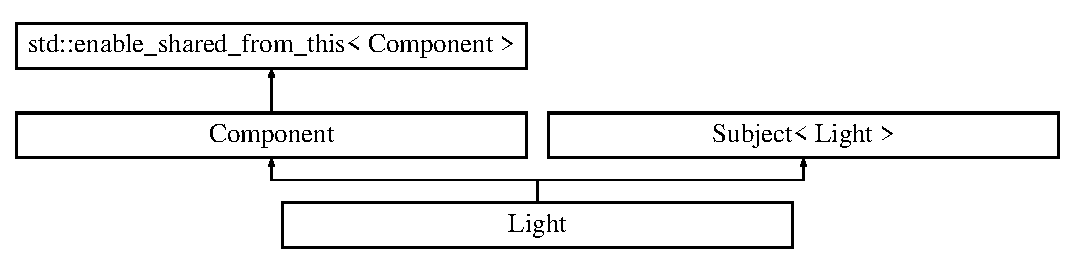
\includegraphics[height=3.000000cm]{class_light}
\end{center}
\end{figure}
\subsection*{Public Member Functions}
\begin{DoxyCompactItemize}
\item 
\hyperlink{class_light_aeb5df09a25a32f19fdffa761268ba24f}{Light} ()
\item 
\hyperlink{class_light_aed70489514bbca33c1c47be11ee5d016}{Light} (glm\+::vec3 color)
\item 
\hyperlink{class_light_ad0e59fad13bb6cfadc25b2c477e9ddc7}{$\sim$\+Light} ()
\item 
glm\+::vec3 \hyperlink{class_light_afcf6054826dc365ca58126c582b71b7a}{get\+Color} ()
\item 
void \hyperlink{class_light_a6dcff3d6e3d90d6d34f5a08e60567f31}{set\+Color} (glm\+::vec3)
\item 
virtual void \hyperlink{class_light_a2c59296fb881070f1e7064ec3ccd4d3d}{init} () override
\item 
virtual void \hyperlink{class_light_a5068d4a5fa02cd63a693030dc4a359fe}{destroy} () override
\item 
virtual shared\+\_\+ptr$<$ \hyperlink{class_component}{Component} $>$ \hyperlink{class_light_ae8747116c592100394c89f76035725e5}{clone} () override
\item 
virtual shared\+\_\+ptr$<$ \hyperlink{class_component_description}{Component\+Description} $>$ \hyperlink{group__serialization__functions_gab8f75c87a12c9eed1fbb3534b516799c}{get\+Component\+Description} () override
\item 
virtual void \hyperlink{group__serialization__functions_ga15349b8cfad97f209ae6ceb0d329bc34}{deserialize} (shared\+\_\+ptr$<$ \hyperlink{class_component_description}{Component\+Description} $>$ desc) override
\end{DoxyCompactItemize}
\subsection*{Additional Inherited Members}


\subsection{Detailed Description}
\hyperlink{class_light}{Light} \hyperlink{class_component}{Component}. This component adds \hyperlink{class_light}{Light} behaviour to a game actor. For now the \hyperlink{class_light}{Light} component behaves like point light and is very very basic There are no shadows currently. 

\subsection{Constructor \& Destructor Documentation}
\hypertarget{class_light_aeb5df09a25a32f19fdffa761268ba24f}{}\index{Light@{Light}!Light@{Light}}
\index{Light@{Light}!Light@{Light}}
\subsubsection[{Light()}]{\setlength{\rightskip}{0pt plus 5cm}Light\+::\+Light (
\begin{DoxyParamCaption}
{}
\end{DoxyParamCaption}
)}\label{class_light_aeb5df09a25a32f19fdffa761268ba24f}
Default Constructor. White \hyperlink{class_light}{Light} \hypertarget{class_light_aed70489514bbca33c1c47be11ee5d016}{}\index{Light@{Light}!Light@{Light}}
\index{Light@{Light}!Light@{Light}}
\subsubsection[{Light(glm\+::vec3 color)}]{\setlength{\rightskip}{0pt plus 5cm}Light\+::\+Light (
\begin{DoxyParamCaption}
\item[{glm\+::vec3}]{c}
\end{DoxyParamCaption}
)}\label{class_light_aed70489514bbca33c1c47be11ee5d016}
Default Constructor. Colored \hyperlink{class_light}{Light} \hypertarget{class_light_ad0e59fad13bb6cfadc25b2c477e9ddc7}{}\index{Light@{Light}!````~Light@{$\sim$\+Light}}
\index{````~Light@{$\sim$\+Light}!Light@{Light}}
\subsubsection[{$\sim$\+Light()}]{\setlength{\rightskip}{0pt plus 5cm}Light\+::$\sim$\+Light (
\begin{DoxyParamCaption}
{}
\end{DoxyParamCaption}
)}\label{class_light_ad0e59fad13bb6cfadc25b2c477e9ddc7}
Default Destructor 

\subsection{Member Function Documentation}
\hypertarget{class_light_ae8747116c592100394c89f76035725e5}{}\index{Light@{Light}!clone@{clone}}
\index{clone@{clone}!Light@{Light}}
\subsubsection[{clone() override}]{\setlength{\rightskip}{0pt plus 5cm}shared\+\_\+ptr$<$ {\bf Component} $>$ Light\+::clone (
\begin{DoxyParamCaption}
{}
\end{DoxyParamCaption}
)\hspace{0.3cm}{\ttfamily [override]}, {\ttfamily [virtual]}}\label{class_light_ae8747116c592100394c89f76035725e5}
Clones current component (Prototype Design Pattern) \begin{DoxyReturn}{Returns}
shared\+\_\+ptr to cloned \hyperlink{class_light}{Light} \hyperlink{class_component}{Component} 
\end{DoxyReturn}


Implements \hyperlink{class_component_a74c984bd819bbef16fd4f306a90d34fe}{Component}.

\hypertarget{class_light_a5068d4a5fa02cd63a693030dc4a359fe}{}\index{Light@{Light}!destroy@{destroy}}
\index{destroy@{destroy}!Light@{Light}}
\subsubsection[{destroy() override}]{\setlength{\rightskip}{0pt plus 5cm}void Light\+::destroy (
\begin{DoxyParamCaption}
{}
\end{DoxyParamCaption}
)\hspace{0.3cm}{\ttfamily [override]}, {\ttfamily [virtual]}}\label{class_light_a5068d4a5fa02cd63a693030dc4a359fe}
\hyperlink{class_component}{Component} destroy override. Notifies that this light has been destroyed 

Reimplemented from \hyperlink{class_component_a77b8fff56ddce5dd0b4a9dabb0b5202b}{Component}.

\hypertarget{class_light_afcf6054826dc365ca58126c582b71b7a}{}\index{Light@{Light}!get\+Color@{get\+Color}}
\index{get\+Color@{get\+Color}!Light@{Light}}
\subsubsection[{get\+Color()}]{\setlength{\rightskip}{0pt plus 5cm}glm\+::vec3 Light\+::get\+Color (
\begin{DoxyParamCaption}
{}
\end{DoxyParamCaption}
)}\label{class_light_afcf6054826dc365ca58126c582b71b7a}
color setter \hypertarget{class_light_a2c59296fb881070f1e7064ec3ccd4d3d}{}\index{Light@{Light}!init@{init}}
\index{init@{init}!Light@{Light}}
\subsubsection[{init() override}]{\setlength{\rightskip}{0pt plus 5cm}void Light\+::init (
\begin{DoxyParamCaption}
{}
\end{DoxyParamCaption}
)\hspace{0.3cm}{\ttfamily [override]}, {\ttfamily [virtual]}}\label{class_light_a2c59296fb881070f1e7064ec3ccd4d3d}
\hyperlink{class_component}{Component} init override. Notifies that a new light has been created 

Reimplemented from \hyperlink{class_component_a162f8cdc070537a71f2ad0b5e763b86f}{Component}.

\hypertarget{class_light_a6dcff3d6e3d90d6d34f5a08e60567f31}{}\index{Light@{Light}!set\+Color@{set\+Color}}
\index{set\+Color@{set\+Color}!Light@{Light}}
\subsubsection[{set\+Color(glm\+::vec3)}]{\setlength{\rightskip}{0pt plus 5cm}void Light\+::set\+Color (
\begin{DoxyParamCaption}
\item[{glm\+::vec3}]{color}
\end{DoxyParamCaption}
)}\label{class_light_a6dcff3d6e3d90d6d34f5a08e60567f31}
color setter 

The documentation for this class was generated from the following files\+:\begin{DoxyCompactItemize}
\item 
/\+Users/guilherme\+\_\+cunha/\+Dev/\+G\+I\+T\+H\+U\+B/\+G\+U\+Inity/\+Source/Light.\+hpp\item 
/\+Users/guilherme\+\_\+cunha/\+Dev/\+G\+I\+T\+H\+U\+B/\+G\+U\+Inity/\+Source/Light.\+cpp\end{DoxyCompactItemize}

\hypertarget{class_light_description}{}\section{Light\+Description Class Reference}
\label{class_light_description}\index{Light\+Description@{Light\+Description}}
Inheritance diagram for Light\+Description\+:\begin{figure}[H]
\begin{center}
\leavevmode
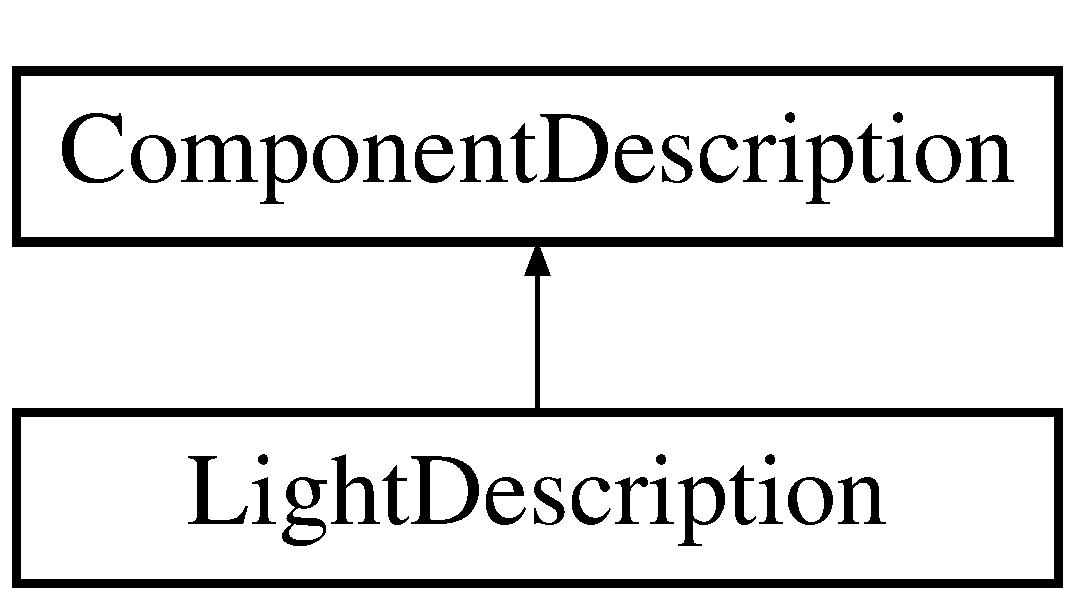
\includegraphics[height=2.000000cm]{class_light_description}
\end{center}
\end{figure}
\subsection*{Public Member Functions}
\begin{DoxyCompactItemize}
\item 
\hypertarget{class_light_description_a216ef61130302902263498c87e7f17f9}{}{\bfseries Light\+Description} (glm\+::vec3 c)\label{class_light_description_a216ef61130302902263498c87e7f17f9}

\end{DoxyCompactItemize}
\subsection*{Public Attributes}
\begin{DoxyCompactItemize}
\item 
\hypertarget{class_light_description_ae85428dbc4e27aca3038a8caaaf73d4e}{}glm\+::vec3 {\bfseries color}\label{class_light_description_ae85428dbc4e27aca3038a8caaaf73d4e}

\end{DoxyCompactItemize}


The documentation for this class was generated from the following file\+:\begin{DoxyCompactItemize}
\item 
/\+Users/guilherme\+\_\+cunha/\+Dev/\+G\+I\+T\+H\+U\+B/\+G\+U\+Inity/\+Source/Serialization\+Structs.\+hpp\end{DoxyCompactItemize}

\hypertarget{class_material}{}\section{Material Class Reference}
\label{class_material}\index{Material@{Material}}


{\ttfamily \#include $<$Material.\+hpp$>$}

Inheritance diagram for Material\+:\begin{figure}[H]
\begin{center}
\leavevmode
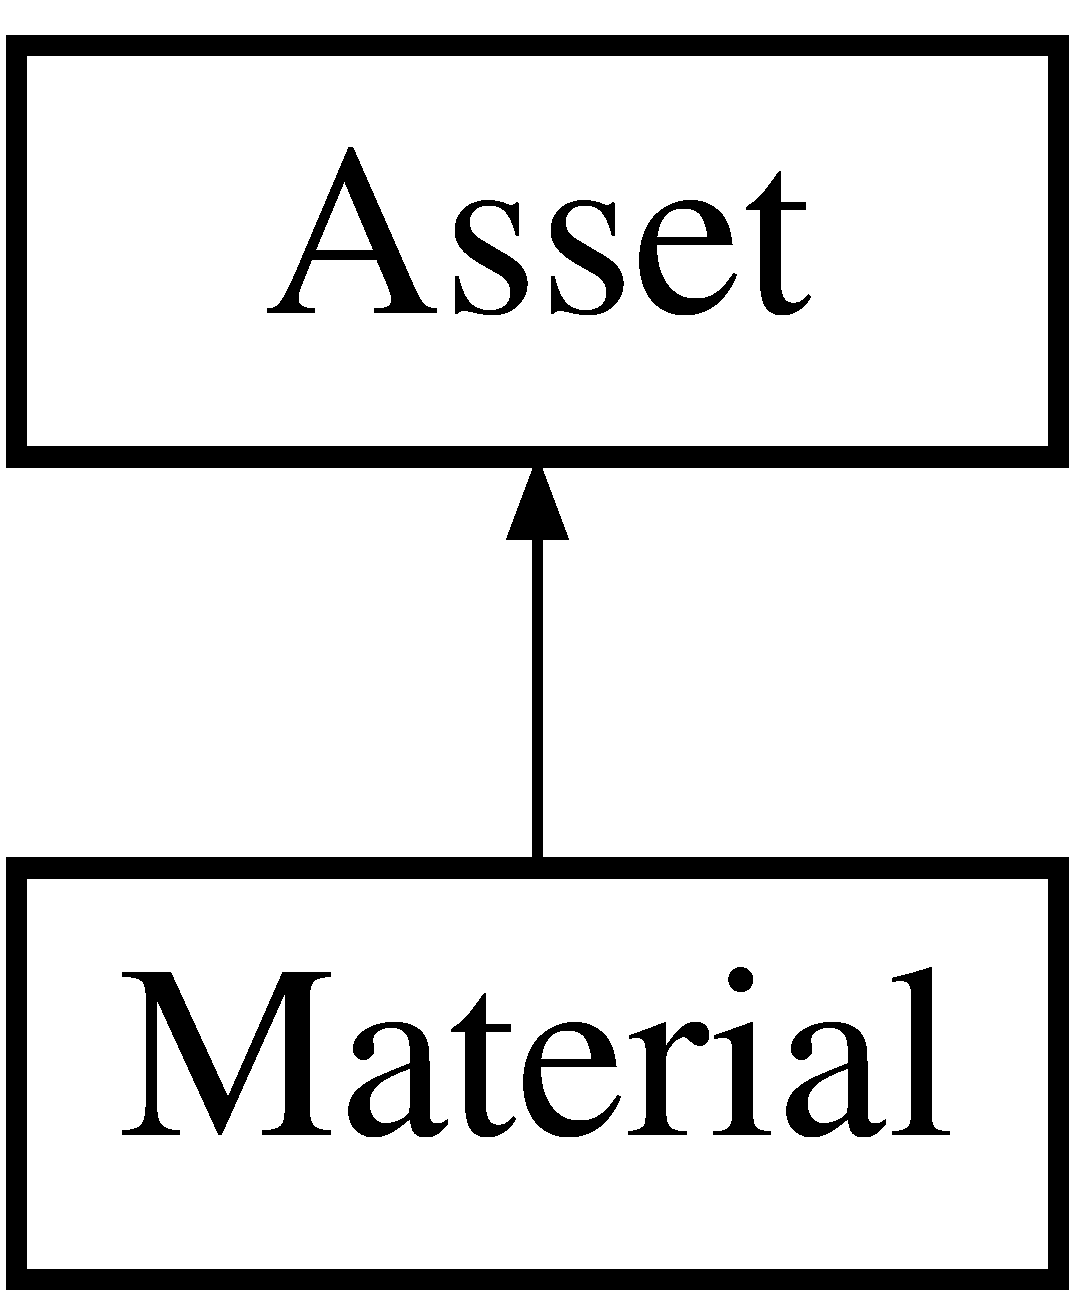
\includegraphics[height=2.000000cm]{class_material}
\end{center}
\end{figure}
\subsection*{Public Types}
\begin{DoxyCompactItemize}
\item 
\hypertarget{class_material_a3bfabbc4ad755103c699c24723a9b995}{}typedef pair$<$ string, shared\+\_\+ptr$<$ \hyperlink{class_texture}{Texture} $>$ $>$ {\bfseries String\+Tex\+Pair}\label{class_material_a3bfabbc4ad755103c699c24723a9b995}

\item 
\hypertarget{class_material_a1543230ce172cd78e40f09caf3ea316b}{}typedef pair$<$ string, glm\+::vec4 $>$ {\bfseries String\+Vec4\+Pair}\label{class_material_a1543230ce172cd78e40f09caf3ea316b}

\end{DoxyCompactItemize}
\subsection*{Public Member Functions}
\begin{DoxyCompactItemize}
\item 
\hyperlink{class_material_a137e987401b63eb7c6c27c3e38bc74b5}{Material} ()
\item 
\hyperlink{class_material_a848e92f90d11160cc3e1242364fbc90f}{Material} (shared\+\_\+ptr$<$ \hyperlink{class_shader}{Shader} $>$ s)
\item 
virtual \hyperlink{class_material_a2c19452d71f54075df8f5405b03129f4}{$\sim$\+Material} ()
\item 
void \hyperlink{class_material_aa9ae26fd244e24eefd45d3bb052cd389}{set\+Shader} (shared\+\_\+ptr$<$ \hyperlink{class_shader}{Shader} $>$ shader)
\item 
shared\+\_\+ptr$<$ \hyperlink{class_shader}{Shader} $>$ \hyperlink{class_material_a4e7dd43b73e383064711a6fbeaa2cc93}{get\+Shader} () const 
\item 
G\+Luint \hyperlink{class_material_ab219530974ad3b8af237ed6e49412bce}{get\+Shader\+Program} ()
\item 
bool \hyperlink{class_material_ac6c1b9f3aa377b9db847bc6d4b22e3e9}{param\+Exists} (string param\+Name)
\item 
void \hyperlink{class_material_a4580ed8224b233f97e5bf2c3ee50eff8}{set\+Param\+Vec4} (string param\+Name, const glm\+::vec4 \&param\+Value)
\item 
void \hyperlink{class_material_a1a6c5fa9ce43ed14f42e5e8bab8b5d61}{set\+Param\+Float} (string param\+Name, float param\+Value)
\item 
void \hyperlink{class_material_a8b9da6d00b1f1bac06f12bb4be8c22d8}{set\+Param\+Texture} (string param\+Name, shared\+\_\+ptr$<$ \hyperlink{class_texture}{Texture} $>$ param\+Value)
\item 
vector$<$ String\+Tex\+Pair $>$ \hyperlink{class_material_aeec2f485d8d0194f87aca6666017f314}{get\+All\+Texture\+Params} ()
\item 
vector$<$ String\+Vec4\+Pair $>$ \hyperlink{class_material_a1d90151378394843fd0c19e08365c4f1}{get\+All\+Vec4\+Params} ()
\end{DoxyCompactItemize}


\subsection{Detailed Description}
\hyperlink{class_material}{Material} is an \hyperlink{class_asset}{Asset} that allows the same shader to be used several times with different parameters. For example, a Textured Diffuse \hyperlink{class_shader}{Shader} could be use for both a crate and the floor, the only thing that changes is the \hyperlink{class_texture}{Texture}.

Currently, the only parameter supported by Shaders and therefore Materials is the \hyperlink{class_texture}{Texture} type. 

\subsection{Constructor \& Destructor Documentation}
\hypertarget{class_material_a137e987401b63eb7c6c27c3e38bc74b5}{}\index{Material@{Material}!Material@{Material}}
\index{Material@{Material}!Material@{Material}}
\subsubsection[{Material()}]{\setlength{\rightskip}{0pt plus 5cm}Material\+::\+Material (
\begin{DoxyParamCaption}
{}
\end{DoxyParamCaption}
)}\label{class_material_a137e987401b63eb7c6c27c3e38bc74b5}
Default Constructor \hypertarget{class_material_a848e92f90d11160cc3e1242364fbc90f}{}\index{Material@{Material}!Material@{Material}}
\index{Material@{Material}!Material@{Material}}
\subsubsection[{Material(shared\+\_\+ptr$<$ Shader $>$ s)}]{\setlength{\rightskip}{0pt plus 5cm}Material\+::\+Material (
\begin{DoxyParamCaption}
\item[{shared\+\_\+ptr$<$ {\bf Shader} $>$}]{shader}
\end{DoxyParamCaption}
)}\label{class_material_a848e92f90d11160cc3e1242364fbc90f}
Constructor for a \hyperlink{class_shader}{Shader} \hypertarget{class_material_a2c19452d71f54075df8f5405b03129f4}{}\index{Material@{Material}!````~Material@{$\sim$\+Material}}
\index{````~Material@{$\sim$\+Material}!Material@{Material}}
\subsubsection[{$\sim$\+Material()}]{\setlength{\rightskip}{0pt plus 5cm}Material\+::$\sim$\+Material (
\begin{DoxyParamCaption}
{}
\end{DoxyParamCaption}
)\hspace{0.3cm}{\ttfamily [virtual]}}\label{class_material_a2c19452d71f54075df8f5405b03129f4}
Default Destructor. Virtual because inherits from \hyperlink{class_asset}{Asset} 

\subsection{Member Function Documentation}
\hypertarget{class_material_aeec2f485d8d0194f87aca6666017f314}{}\index{Material@{Material}!get\+All\+Texture\+Params@{get\+All\+Texture\+Params}}
\index{get\+All\+Texture\+Params@{get\+All\+Texture\+Params}!Material@{Material}}
\subsubsection[{get\+All\+Texture\+Params()}]{\setlength{\rightskip}{0pt plus 5cm}vector$<$ Material\+::\+String\+Tex\+Pair $>$ Material\+::get\+All\+Texture\+Params (
\begin{DoxyParamCaption}
{}
\end{DoxyParamCaption}
)}\label{class_material_aeec2f485d8d0194f87aca6666017f314}
Gets all \hyperlink{class_texture}{Texture} params \hypertarget{class_material_a1d90151378394843fd0c19e08365c4f1}{}\index{Material@{Material}!get\+All\+Vec4\+Params@{get\+All\+Vec4\+Params}}
\index{get\+All\+Vec4\+Params@{get\+All\+Vec4\+Params}!Material@{Material}}
\subsubsection[{get\+All\+Vec4\+Params()}]{\setlength{\rightskip}{0pt plus 5cm}vector$<$ Material\+::\+String\+Vec4\+Pair $>$ Material\+::get\+All\+Vec4\+Params (
\begin{DoxyParamCaption}
{}
\end{DoxyParamCaption}
)}\label{class_material_a1d90151378394843fd0c19e08365c4f1}
Gets all Vec4 params

Gets all Vec3 params \hypertarget{class_material_a4e7dd43b73e383064711a6fbeaa2cc93}{}\index{Material@{Material}!get\+Shader@{get\+Shader}}
\index{get\+Shader@{get\+Shader}!Material@{Material}}
\subsubsection[{get\+Shader() const }]{\setlength{\rightskip}{0pt plus 5cm}shared\+\_\+ptr$<$ {\bf Shader} $>$ Material\+::get\+Shader (
\begin{DoxyParamCaption}
{}
\end{DoxyParamCaption}
) const}\label{class_material_a4e7dd43b73e383064711a6fbeaa2cc93}
shader Getter \hypertarget{class_material_ab219530974ad3b8af237ed6e49412bce}{}\index{Material@{Material}!get\+Shader\+Program@{get\+Shader\+Program}}
\index{get\+Shader\+Program@{get\+Shader\+Program}!Material@{Material}}
\subsubsection[{get\+Shader\+Program()}]{\setlength{\rightskip}{0pt plus 5cm}G\+Luint Material\+::get\+Shader\+Program (
\begin{DoxyParamCaption}
{}
\end{DoxyParamCaption}
)}\label{class_material_ab219530974ad3b8af237ed6e49412bce}
Get the shader program \hypertarget{class_material_ac6c1b9f3aa377b9db847bc6d4b22e3e9}{}\index{Material@{Material}!param\+Exists@{param\+Exists}}
\index{param\+Exists@{param\+Exists}!Material@{Material}}
\subsubsection[{param\+Exists(string param\+Name)}]{\setlength{\rightskip}{0pt plus 5cm}bool Material\+::param\+Exists (
\begin{DoxyParamCaption}
\item[{string}]{param\+Name}
\end{DoxyParamCaption}
)}\label{class_material_ac6c1b9f3aa377b9db847bc6d4b22e3e9}
Checks if param exists on params map \hypertarget{class_material_a1a6c5fa9ce43ed14f42e5e8bab8b5d61}{}\index{Material@{Material}!set\+Param\+Float@{set\+Param\+Float}}
\index{set\+Param\+Float@{set\+Param\+Float}!Material@{Material}}
\subsubsection[{set\+Param\+Float(string param\+Name, float param\+Value)}]{\setlength{\rightskip}{0pt plus 5cm}void Material\+::set\+Param\+Float (
\begin{DoxyParamCaption}
\item[{string}]{param\+Name, }
\item[{float}]{param\+Value}
\end{DoxyParamCaption}
)}\label{class_material_a1a6c5fa9ce43ed14f42e5e8bab8b5d61}
Set a float param that has name param\+Name \hypertarget{class_material_a8b9da6d00b1f1bac06f12bb4be8c22d8}{}\index{Material@{Material}!set\+Param\+Texture@{set\+Param\+Texture}}
\index{set\+Param\+Texture@{set\+Param\+Texture}!Material@{Material}}
\subsubsection[{set\+Param\+Texture(string param\+Name, shared\+\_\+ptr$<$ Texture $>$ param\+Value)}]{\setlength{\rightskip}{0pt plus 5cm}void Material\+::set\+Param\+Texture (
\begin{DoxyParamCaption}
\item[{string}]{param\+Name, }
\item[{shared\+\_\+ptr$<$ {\bf Texture} $>$}]{param\+Value}
\end{DoxyParamCaption}
)}\label{class_material_a8b9da6d00b1f1bac06f12bb4be8c22d8}
Set a \hyperlink{class_texture}{Texture} param that has name param\+Name \hypertarget{class_material_a4580ed8224b233f97e5bf2c3ee50eff8}{}\index{Material@{Material}!set\+Param\+Vec4@{set\+Param\+Vec4}}
\index{set\+Param\+Vec4@{set\+Param\+Vec4}!Material@{Material}}
\subsubsection[{set\+Param\+Vec4(string param\+Name, const glm\+::vec4 \&param\+Value)}]{\setlength{\rightskip}{0pt plus 5cm}void Material\+::set\+Param\+Vec4 (
\begin{DoxyParamCaption}
\item[{string}]{param\+Name, }
\item[{const glm\+::vec4 \&}]{param\+Value}
\end{DoxyParamCaption}
)}\label{class_material_a4580ed8224b233f97e5bf2c3ee50eff8}
Set a vec4 param that has name param\+Name \hypertarget{class_material_aa9ae26fd244e24eefd45d3bb052cd389}{}\index{Material@{Material}!set\+Shader@{set\+Shader}}
\index{set\+Shader@{set\+Shader}!Material@{Material}}
\subsubsection[{set\+Shader(shared\+\_\+ptr$<$ Shader $>$ shader)}]{\setlength{\rightskip}{0pt plus 5cm}void Material\+::set\+Shader (
\begin{DoxyParamCaption}
\item[{shared\+\_\+ptr$<$ {\bf Shader} $>$}]{shader}
\end{DoxyParamCaption}
)}\label{class_material_aa9ae26fd244e24eefd45d3bb052cd389}
shader Setter 

The documentation for this class was generated from the following files\+:\begin{DoxyCompactItemize}
\item 
/\+Users/guilherme\+\_\+cunha/\+Dev/\+G\+I\+T\+H\+U\+B/\+G\+U\+Inity/\+Source/Material.\+hpp\item 
/\+Users/guilherme\+\_\+cunha/\+Dev/\+G\+I\+T\+H\+U\+B/\+G\+U\+Inity/\+Source/Material.\+cpp\end{DoxyCompactItemize}

\hypertarget{struct_member_info}{}\section{Member\+Info Struct Reference}
\label{struct_member_info}\index{Member\+Info@{Member\+Info}}
\subsection*{Public Member Functions}
\begin{DoxyCompactItemize}
\item 
\hypertarget{struct_member_info_a3ed923c05fa1e724c9118bb98f1d6658}{}{\bfseries Member\+Info} (string type, string name)\label{struct_member_info_a3ed923c05fa1e724c9118bb98f1d6658}

\end{DoxyCompactItemize}
\subsection*{Public Attributes}
\begin{DoxyCompactItemize}
\item 
\hypertarget{struct_member_info_ac5de9c4eebf0a9b11b20138c366337c3}{}string {\bfseries name}\label{struct_member_info_ac5de9c4eebf0a9b11b20138c366337c3}

\item 
\hypertarget{struct_member_info_a7bf767382190d02cce54f319dd0e1f2e}{}string {\bfseries type}\label{struct_member_info_a7bf767382190d02cce54f319dd0e1f2e}

\end{DoxyCompactItemize}


The documentation for this struct was generated from the following file\+:\begin{DoxyCompactItemize}
\item 
/\+Users/guilherme\+\_\+cunha/\+Dev/\+G\+I\+T\+H\+U\+B/\+G\+U\+Inity/\+Source/Reflection\+Test.\+h\end{DoxyCompactItemize}

\hypertarget{class_mesh}{}\section{Mesh Class Reference}
\label{class_mesh}\index{Mesh@{Mesh}}


{\ttfamily \#include $<$Mesh.\+hpp$>$}

Inheritance diagram for Mesh\+:\begin{figure}[H]
\begin{center}
\leavevmode
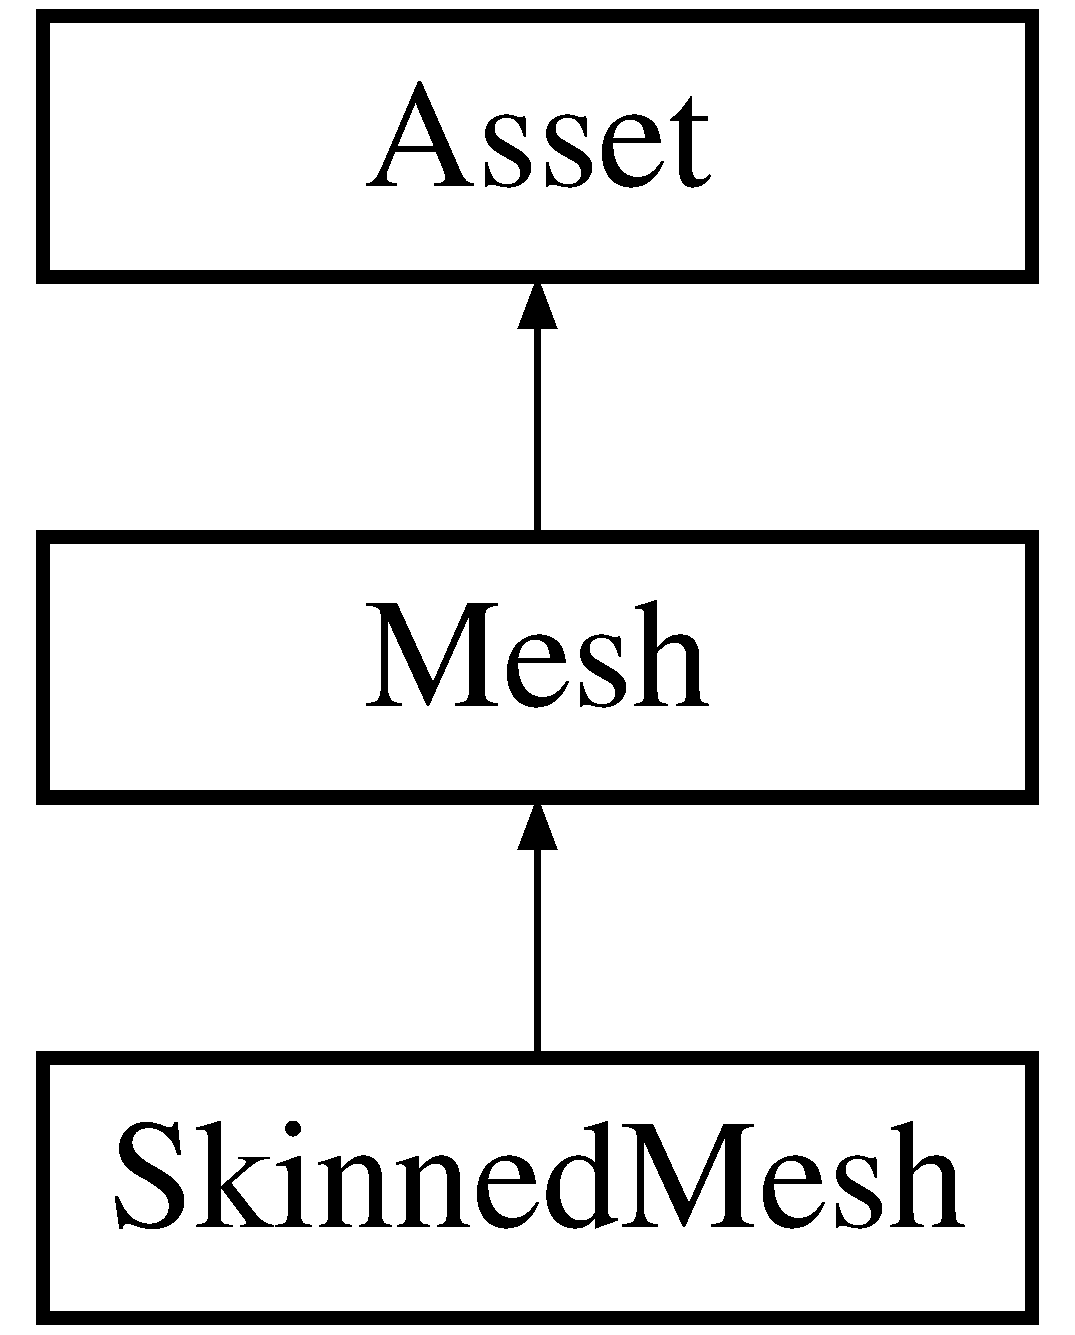
\includegraphics[height=3.000000cm]{class_mesh}
\end{center}
\end{figure}
\subsection*{Public Member Functions}
\begin{DoxyCompactItemize}
\item 
\hyperlink{class_mesh_a2af137f1571af89172b9c102302c416b}{Mesh} ()
\item 
\hyperlink{class_mesh_a6001afbb24255fe880ae5d609bfb7cd2}{Mesh} (float $\ast$indices, float $\ast$normal\+Points, float $\ast$uv, unsigned int $\ast$\hyperlink{class_mesh_ad41061e78a04735d509e548141d43a49}{triangles}, int n\+Points, int n\+Triangles)
\item 
\hyperlink{class_mesh_a8d847ce8604fd8f6e84f97acbf481503}{Mesh} (vector$<$ \hyperlink{struct_mesh_vertex}{Mesh\+Vertex} $>$ vertex, vector$<$ unsigned short $>$ \hyperlink{class_mesh_ad41061e78a04735d509e548141d43a49}{triangles})
\item 
\hyperlink{class_mesh_a6cc43f6b68cf3fd6881f17ba78ab089d}{Mesh} (vector$<$ glm\+::vec3 $>$ vertices, vector$<$ int $>$ used\+Index, vector$<$ int $>$ used\+Tris)
\item 
virtual \hyperlink{class_mesh_a5efe4da1a4c0971cfb037bd70304c303}{$\sim$\+Mesh} ()
\item 
void \hyperlink{class_mesh_a97cadeaf5ef95c8a35d5eb2ded9ca73c}{set\+Scale\+Factor} (float f)
\item 
float \hyperlink{class_mesh_a4d70792ba5142b0d663d39443917da58}{get\+Scale\+Factor} ()
\item 
glm\+::vec3 \hyperlink{class_mesh_a563db5002a111f742d2939f4a432d4ef}{get\+Bounds\+Min} ()
\item 
glm\+::vec3 \hyperlink{class_mesh_a47a810bcf709c90d36e453af2bbe11c0}{get\+Bounds\+Max} ()
\item 
glm\+::vec3 \hyperlink{class_mesh_aa93bf2f2ae299b9987d083e8549c4d20}{get\+Average\+Center} ()
\item 
float \hyperlink{class_mesh_a891595d8aa7ca667df30d03d14dae0f3}{get\+Vertex\+Array\+I\+D} ()
\item 
float \hyperlink{class_mesh_a170e6001bf96cc741afe7d9425b2f440}{get\+Vertex\+Buffer} ()
\item 
float \hyperlink{class_mesh_a111b94c34d164c15dbe391940e0202c1}{get\+Triangles\+Buffer} ()
\item 
int \hyperlink{class_mesh_ae3957c15ba7d62336640b822d2c41161}{get\+Triangles\+Count} ()
\item 
int \hyperlink{class_mesh_a1394a088d7e4bb7a82ca1799098fe025}{get\+Vertices\+Count} ()
\item 
void \hyperlink{class_mesh_a571745a25511f03dfb54bb9248ebe0e9}{add\+Vertex} (glm\+::vec3 position, glm\+::vec2 uv, glm\+::vec3 normal)
\item 
void \hyperlink{class_mesh_a317d2916ce9675ef1b4d1b70f9ef62a6}{add\+Triangle} (int vertex\+Index)
\item 
\hypertarget{class_mesh_a57dd31edc88c118fddc8d60c4fe08efd}{}void {\bfseries set\+Vertices} (vector$<$ \hyperlink{struct_mesh_vertex}{Mesh\+Vertex} $>$ \hyperlink{class_mesh_a91899b71cdc960ef485b07ffcd0c0cd6}{mesh\+Vertices})\label{class_mesh_a57dd31edc88c118fddc8d60c4fe08efd}

\item 
\hypertarget{class_mesh_a30ac5bc862b6c2f6c681c586a9d5ff34}{}void {\bfseries set\+Triangles} (vector$<$ unsigned short $>$ \hyperlink{class_mesh_ad41061e78a04735d509e548141d43a49}{triangles})\label{class_mesh_a30ac5bc862b6c2f6c681c586a9d5ff34}

\item 
void \hyperlink{class_mesh_a508c26a83f4a575f3cdbba07a2118809}{create\+Buffers} ()
\item 
void \hyperlink{class_mesh_a2337847905aa738a21c7b2c459b30bbc}{calculate\+Bounds} ()
\item 
vector$<$ glm\+::vec3 $>$ \hyperlink{class_mesh_abac6433b4de282c3477631e1f00552ee}{get\+Non\+Duplicate\+Mesh\+Vertex} ()
\end{DoxyCompactItemize}
\subsection*{Public Attributes}
\begin{DoxyCompactItemize}
\item 
vector$<$ \hyperlink{struct_mesh_vertex}{Mesh\+Vertex} $>$ \hyperlink{class_mesh_a91899b71cdc960ef485b07ffcd0c0cd6}{mesh\+Vertices}
\item 
vector$<$ unsigned short $>$ \hyperlink{class_mesh_ad41061e78a04735d509e548141d43a49}{triangles}
\item 
G\+Luint \hyperlink{class_mesh_a101a39d88bc5c8d33f0ebd6e77a60129}{vao}
\item 
G\+Luint \hyperlink{class_mesh_a8fb0190a2e74648537e452031c00fb8d}{ibo}
\item 
G\+Luint \hyperlink{class_mesh_ab24bc96d6c0f11d570a193fc133884a7}{mvbo}
\item 
float \hyperlink{class_mesh_a1fc2f16522570f5e3bbed514ac322d9a}{scale\+Factor}
\item 
glm\+::vec3 \hyperlink{class_mesh_a0cb39dfb46a4eb89e748b7966f20e08b}{bounds\+Min}
\item 
glm\+::vec3 \hyperlink{class_mesh_a430e466fef8de4297fb25aa8727b52e3}{bounds\+Max}
\item 
glm\+::vec3 \hyperlink{class_mesh_a666f0d7350993308b29826cf94a86978}{avg\+Center}
\end{DoxyCompactItemize}
\subsection*{Friends}
\begin{DoxyCompactItemize}
\item 
\hypertarget{class_mesh_ac98d07dd8f7b70e16ccb9a01abf56b9c}{}class {\bfseries boost\+::serialization\+::access}\label{class_mesh_ac98d07dd8f7b70e16ccb9a01abf56b9c}

\end{DoxyCompactItemize}


\subsection{Detailed Description}
\hyperlink{class_mesh}{Mesh} is an \hyperlink{class_asset}{Asset} that represents a 3\+D Model. The vertexes are indexed, meaning that they\textquotesingle{}re stored once only and can be referenced in several faces (triangles).

Currently supported features\+: -\/\+Vertex Position -\/\+Vertex U\+V -\/\+Vertex Normal

Animations are N\+O\+T currently supported. 

\subsection{Constructor \& Destructor Documentation}
\hypertarget{class_mesh_a2af137f1571af89172b9c102302c416b}{}\index{Mesh@{Mesh}!Mesh@{Mesh}}
\index{Mesh@{Mesh}!Mesh@{Mesh}}
\subsubsection[{Mesh()}]{\setlength{\rightskip}{0pt plus 5cm}Mesh\+::\+Mesh (
\begin{DoxyParamCaption}
{}
\end{DoxyParamCaption}
)}\label{class_mesh_a2af137f1571af89172b9c102302c416b}
Default Constructor \hypertarget{class_mesh_a6001afbb24255fe880ae5d609bfb7cd2}{}\index{Mesh@{Mesh}!Mesh@{Mesh}}
\index{Mesh@{Mesh}!Mesh@{Mesh}}
\subsubsection[{Mesh(float $\ast$indices, float $\ast$normal\+Points, float $\ast$uv, unsigned int $\ast$triangles, int n\+Points, int n\+Triangles)}]{\setlength{\rightskip}{0pt plus 5cm}Mesh\+::\+Mesh (
\begin{DoxyParamCaption}
\item[{float $\ast$}]{indices, }
\item[{float $\ast$}]{normal\+Points, }
\item[{float $\ast$}]{uv, }
\item[{unsigned int $\ast$}]{triangles, }
\item[{int}]{n\+Points, }
\item[{int}]{n\+Triangles}
\end{DoxyParamCaption}
)}\label{class_mesh_a6001afbb24255fe880ae5d609bfb7cd2}
Constructor from array of indices, normal points, uvs and triangles \hypertarget{class_mesh_a8d847ce8604fd8f6e84f97acbf481503}{}\index{Mesh@{Mesh}!Mesh@{Mesh}}
\index{Mesh@{Mesh}!Mesh@{Mesh}}
\subsubsection[{Mesh(vector$<$ Mesh\+Vertex $>$ vertex, vector$<$ unsigned short $>$ triangles)}]{\setlength{\rightskip}{0pt plus 5cm}Mesh\+::\+Mesh (
\begin{DoxyParamCaption}
\item[{vector$<$ {\bf Mesh\+Vertex} $>$}]{vertex, }
\item[{vector$<$ unsigned short $>$}]{triangles}
\end{DoxyParamCaption}
)}\label{class_mesh_a8d847ce8604fd8f6e84f97acbf481503}
Constructor from vector of \hyperlink{struct_mesh_vertex}{Mesh\+Vertex} and triangles \hypertarget{class_mesh_a6cc43f6b68cf3fd6881f17ba78ab089d}{}\index{Mesh@{Mesh}!Mesh@{Mesh}}
\index{Mesh@{Mesh}!Mesh@{Mesh}}
\subsubsection[{Mesh(vector$<$ glm\+::vec3 $>$ vertices, vector$<$ int $>$ used\+Index, vector$<$ int $>$ used\+Tris)}]{\setlength{\rightskip}{0pt plus 5cm}Mesh\+::\+Mesh (
\begin{DoxyParamCaption}
\item[{vector$<$ glm\+::vec3 $>$}]{vertices, }
\item[{vector$<$ int $>$}]{used\+Index, }
\item[{vector$<$ int $>$}]{used\+Tris}
\end{DoxyParamCaption}
)}\label{class_mesh_a6cc43f6b68cf3fd6881f17ba78ab089d}
Constructor from vector of \hyperlink{struct_mesh_vertex}{Mesh\+Vertex}, subset of used Indexes and triangles \hypertarget{class_mesh_a5efe4da1a4c0971cfb037bd70304c303}{}\index{Mesh@{Mesh}!````~Mesh@{$\sim$\+Mesh}}
\index{````~Mesh@{$\sim$\+Mesh}!Mesh@{Mesh}}
\subsubsection[{$\sim$\+Mesh()}]{\setlength{\rightskip}{0pt plus 5cm}Mesh\+::$\sim$\+Mesh (
\begin{DoxyParamCaption}
{}
\end{DoxyParamCaption}
)\hspace{0.3cm}{\ttfamily [virtual]}}\label{class_mesh_a5efe4da1a4c0971cfb037bd70304c303}
Default Destructor 

\subsection{Member Function Documentation}
\hypertarget{class_mesh_a317d2916ce9675ef1b4d1b70f9ef62a6}{}\index{Mesh@{Mesh}!add\+Triangle@{add\+Triangle}}
\index{add\+Triangle@{add\+Triangle}!Mesh@{Mesh}}
\subsubsection[{add\+Triangle(int vertex\+Index)}]{\setlength{\rightskip}{0pt plus 5cm}void Mesh\+::add\+Triangle (
\begin{DoxyParamCaption}
\item[{int}]{vertex\+Index}
\end{DoxyParamCaption}
)}\label{class_mesh_a317d2916ce9675ef1b4d1b70f9ef62a6}
Adds a new index to the triangles list \hypertarget{class_mesh_a571745a25511f03dfb54bb9248ebe0e9}{}\index{Mesh@{Mesh}!add\+Vertex@{add\+Vertex}}
\index{add\+Vertex@{add\+Vertex}!Mesh@{Mesh}}
\subsubsection[{add\+Vertex(glm\+::vec3 position, glm\+::vec2 uv, glm\+::vec3 normal)}]{\setlength{\rightskip}{0pt plus 5cm}void Mesh\+::add\+Vertex (
\begin{DoxyParamCaption}
\item[{glm\+::vec3}]{position, }
\item[{glm\+::vec2}]{uv, }
\item[{glm\+::vec3}]{normal}
\end{DoxyParamCaption}
)}\label{class_mesh_a571745a25511f03dfb54bb9248ebe0e9}
Adds a new vertex to the mesh \hypertarget{class_mesh_a2337847905aa738a21c7b2c459b30bbc}{}\index{Mesh@{Mesh}!calculate\+Bounds@{calculate\+Bounds}}
\index{calculate\+Bounds@{calculate\+Bounds}!Mesh@{Mesh}}
\subsubsection[{calculate\+Bounds()}]{\setlength{\rightskip}{0pt plus 5cm}void Mesh\+::calculate\+Bounds (
\begin{DoxyParamCaption}
{}
\end{DoxyParamCaption}
)}\label{class_mesh_a2337847905aa738a21c7b2c459b30bbc}
Calculate mesh bounds \hypertarget{class_mesh_a508c26a83f4a575f3cdbba07a2118809}{}\index{Mesh@{Mesh}!create\+Buffers@{create\+Buffers}}
\index{create\+Buffers@{create\+Buffers}!Mesh@{Mesh}}
\subsubsection[{create\+Buffers()}]{\setlength{\rightskip}{0pt plus 5cm}void Mesh\+::create\+Buffers (
\begin{DoxyParamCaption}
{}
\end{DoxyParamCaption}
)}\label{class_mesh_a508c26a83f4a575f3cdbba07a2118809}
Create Open\+G\+L buffers \hypertarget{class_mesh_aa93bf2f2ae299b9987d083e8549c4d20}{}\index{Mesh@{Mesh}!get\+Average\+Center@{get\+Average\+Center}}
\index{get\+Average\+Center@{get\+Average\+Center}!Mesh@{Mesh}}
\subsubsection[{get\+Average\+Center()}]{\setlength{\rightskip}{0pt plus 5cm}glm\+::vec3 Mesh\+::get\+Average\+Center (
\begin{DoxyParamCaption}
{}
\end{DoxyParamCaption}
)}\label{class_mesh_aa93bf2f2ae299b9987d083e8549c4d20}
avg\+Center Getter \hypertarget{class_mesh_a47a810bcf709c90d36e453af2bbe11c0}{}\index{Mesh@{Mesh}!get\+Bounds\+Max@{get\+Bounds\+Max}}
\index{get\+Bounds\+Max@{get\+Bounds\+Max}!Mesh@{Mesh}}
\subsubsection[{get\+Bounds\+Max()}]{\setlength{\rightskip}{0pt plus 5cm}glm\+::vec3 Mesh\+::get\+Bounds\+Max (
\begin{DoxyParamCaption}
{}
\end{DoxyParamCaption}
)}\label{class_mesh_a47a810bcf709c90d36e453af2bbe11c0}
bounds\+Max Getter \hypertarget{class_mesh_a563db5002a111f742d2939f4a432d4ef}{}\index{Mesh@{Mesh}!get\+Bounds\+Min@{get\+Bounds\+Min}}
\index{get\+Bounds\+Min@{get\+Bounds\+Min}!Mesh@{Mesh}}
\subsubsection[{get\+Bounds\+Min()}]{\setlength{\rightskip}{0pt plus 5cm}glm\+::vec3 Mesh\+::get\+Bounds\+Min (
\begin{DoxyParamCaption}
{}
\end{DoxyParamCaption}
)}\label{class_mesh_a563db5002a111f742d2939f4a432d4ef}
bounds\+Min Getter \hypertarget{class_mesh_abac6433b4de282c3477631e1f00552ee}{}\index{Mesh@{Mesh}!get\+Non\+Duplicate\+Mesh\+Vertex@{get\+Non\+Duplicate\+Mesh\+Vertex}}
\index{get\+Non\+Duplicate\+Mesh\+Vertex@{get\+Non\+Duplicate\+Mesh\+Vertex}!Mesh@{Mesh}}
\subsubsection[{get\+Non\+Duplicate\+Mesh\+Vertex()}]{\setlength{\rightskip}{0pt plus 5cm}vector$<$ glm\+::vec3 $>$ Mesh\+::get\+Non\+Duplicate\+Mesh\+Vertex (
\begin{DoxyParamCaption}
{}
\end{DoxyParamCaption}
)}\label{class_mesh_abac6433b4de282c3477631e1f00552ee}
Returns non duplicate mesh vertices based on position only. It does not take into consideration other parameters such as U\+V or normal. This function was used by the Convex\+Hull in \hyperlink{_math_8hpp_source}{Math.\+hpp} \hypertarget{class_mesh_a4d70792ba5142b0d663d39443917da58}{}\index{Mesh@{Mesh}!get\+Scale\+Factor@{get\+Scale\+Factor}}
\index{get\+Scale\+Factor@{get\+Scale\+Factor}!Mesh@{Mesh}}
\subsubsection[{get\+Scale\+Factor()}]{\setlength{\rightskip}{0pt plus 5cm}float Mesh\+::get\+Scale\+Factor (
\begin{DoxyParamCaption}
{}
\end{DoxyParamCaption}
)}\label{class_mesh_a4d70792ba5142b0d663d39443917da58}
scale\+Factor getter \hypertarget{class_mesh_a111b94c34d164c15dbe391940e0202c1}{}\index{Mesh@{Mesh}!get\+Triangles\+Buffer@{get\+Triangles\+Buffer}}
\index{get\+Triangles\+Buffer@{get\+Triangles\+Buffer}!Mesh@{Mesh}}
\subsubsection[{get\+Triangles\+Buffer()}]{\setlength{\rightskip}{0pt plus 5cm}float Mesh\+::get\+Triangles\+Buffer (
\begin{DoxyParamCaption}
{}
\end{DoxyParamCaption}
)}\label{class_mesh_a111b94c34d164c15dbe391940e0202c1}
ibo getter \hypertarget{class_mesh_ae3957c15ba7d62336640b822d2c41161}{}\index{Mesh@{Mesh}!get\+Triangles\+Count@{get\+Triangles\+Count}}
\index{get\+Triangles\+Count@{get\+Triangles\+Count}!Mesh@{Mesh}}
\subsubsection[{get\+Triangles\+Count()}]{\setlength{\rightskip}{0pt plus 5cm}int Mesh\+::get\+Triangles\+Count (
\begin{DoxyParamCaption}
{}
\end{DoxyParamCaption}
)}\label{class_mesh_ae3957c15ba7d62336640b822d2c41161}
Count of triangles list

Count of triangles list getter \hypertarget{class_mesh_a891595d8aa7ca667df30d03d14dae0f3}{}\index{Mesh@{Mesh}!get\+Vertex\+Array\+I\+D@{get\+Vertex\+Array\+I\+D}}
\index{get\+Vertex\+Array\+I\+D@{get\+Vertex\+Array\+I\+D}!Mesh@{Mesh}}
\subsubsection[{get\+Vertex\+Array\+I\+D()}]{\setlength{\rightskip}{0pt plus 5cm}float Mesh\+::get\+Vertex\+Array\+I\+D (
\begin{DoxyParamCaption}
{}
\end{DoxyParamCaption}
)}\label{class_mesh_a891595d8aa7ca667df30d03d14dae0f3}
vao getter \hypertarget{class_mesh_a170e6001bf96cc741afe7d9425b2f440}{}\index{Mesh@{Mesh}!get\+Vertex\+Buffer@{get\+Vertex\+Buffer}}
\index{get\+Vertex\+Buffer@{get\+Vertex\+Buffer}!Mesh@{Mesh}}
\subsubsection[{get\+Vertex\+Buffer()}]{\setlength{\rightskip}{0pt plus 5cm}float Mesh\+::get\+Vertex\+Buffer (
\begin{DoxyParamCaption}
{}
\end{DoxyParamCaption}
)}\label{class_mesh_a170e6001bf96cc741afe7d9425b2f440}
mvbo getter \hypertarget{class_mesh_a1394a088d7e4bb7a82ca1799098fe025}{}\index{Mesh@{Mesh}!get\+Vertices\+Count@{get\+Vertices\+Count}}
\index{get\+Vertices\+Count@{get\+Vertices\+Count}!Mesh@{Mesh}}
\subsubsection[{get\+Vertices\+Count()}]{\setlength{\rightskip}{0pt plus 5cm}int Mesh\+::get\+Vertices\+Count (
\begin{DoxyParamCaption}
{}
\end{DoxyParamCaption}
)}\label{class_mesh_a1394a088d7e4bb7a82ca1799098fe025}
Count of \hyperlink{class_mesh}{Mesh} Vertices \hypertarget{class_mesh_a97cadeaf5ef95c8a35d5eb2ded9ca73c}{}\index{Mesh@{Mesh}!set\+Scale\+Factor@{set\+Scale\+Factor}}
\index{set\+Scale\+Factor@{set\+Scale\+Factor}!Mesh@{Mesh}}
\subsubsection[{set\+Scale\+Factor(float f)}]{\setlength{\rightskip}{0pt plus 5cm}void Mesh\+::set\+Scale\+Factor (
\begin{DoxyParamCaption}
\item[{float}]{f}
\end{DoxyParamCaption}
)}\label{class_mesh_a97cadeaf5ef95c8a35d5eb2ded9ca73c}
scale\+Factor Setter 

\subsection{Member Data Documentation}
\hypertarget{class_mesh_a666f0d7350993308b29826cf94a86978}{}\index{Mesh@{Mesh}!avg\+Center@{avg\+Center}}
\index{avg\+Center@{avg\+Center}!Mesh@{Mesh}}
\subsubsection[{avg\+Center}]{\setlength{\rightskip}{0pt plus 5cm}glm\+::vec3 Mesh\+::avg\+Center}\label{class_mesh_a666f0d7350993308b29826cf94a86978}
Average center of the mesh \hypertarget{class_mesh_a430e466fef8de4297fb25aa8727b52e3}{}\index{Mesh@{Mesh}!bounds\+Max@{bounds\+Max}}
\index{bounds\+Max@{bounds\+Max}!Mesh@{Mesh}}
\subsubsection[{bounds\+Max}]{\setlength{\rightskip}{0pt plus 5cm}glm\+::vec3 Mesh\+::bounds\+Max}\label{class_mesh_a430e466fef8de4297fb25aa8727b52e3}
Max bounds of the mesh \hypertarget{class_mesh_a0cb39dfb46a4eb89e748b7966f20e08b}{}\index{Mesh@{Mesh}!bounds\+Min@{bounds\+Min}}
\index{bounds\+Min@{bounds\+Min}!Mesh@{Mesh}}
\subsubsection[{bounds\+Min}]{\setlength{\rightskip}{0pt plus 5cm}glm\+::vec3 Mesh\+::bounds\+Min}\label{class_mesh_a0cb39dfb46a4eb89e748b7966f20e08b}
Min bounds of the mesh \hypertarget{class_mesh_a8fb0190a2e74648537e452031c00fb8d}{}\index{Mesh@{Mesh}!ibo@{ibo}}
\index{ibo@{ibo}!Mesh@{Mesh}}
\subsubsection[{ibo}]{\setlength{\rightskip}{0pt plus 5cm}G\+Luint Mesh\+::ibo}\label{class_mesh_a8fb0190a2e74648537e452031c00fb8d}
Triangles array \hypertarget{class_mesh_a91899b71cdc960ef485b07ffcd0c0cd6}{}\index{Mesh@{Mesh}!mesh\+Vertices@{mesh\+Vertices}}
\index{mesh\+Vertices@{mesh\+Vertices}!Mesh@{Mesh}}
\subsubsection[{mesh\+Vertices}]{\setlength{\rightskip}{0pt plus 5cm}vector$<${\bf Mesh\+Vertex}$>$ Mesh\+::mesh\+Vertices}\label{class_mesh_a91899b71cdc960ef485b07ffcd0c0cd6}
The vertices data \hypertarget{class_mesh_ab24bc96d6c0f11d570a193fc133884a7}{}\index{Mesh@{Mesh}!mvbo@{mvbo}}
\index{mvbo@{mvbo}!Mesh@{Mesh}}
\subsubsection[{mvbo}]{\setlength{\rightskip}{0pt plus 5cm}G\+Luint Mesh\+::mvbo}\label{class_mesh_ab24bc96d6c0f11d570a193fc133884a7}
Vertex data array \hypertarget{class_mesh_a1fc2f16522570f5e3bbed514ac322d9a}{}\index{Mesh@{Mesh}!scale\+Factor@{scale\+Factor}}
\index{scale\+Factor@{scale\+Factor}!Mesh@{Mesh}}
\subsubsection[{scale\+Factor}]{\setlength{\rightskip}{0pt plus 5cm}float Mesh\+::scale\+Factor}\label{class_mesh_a1fc2f16522570f5e3bbed514ac322d9a}
Scale factor of the mesh \hypertarget{class_mesh_ad41061e78a04735d509e548141d43a49}{}\index{Mesh@{Mesh}!triangles@{triangles}}
\index{triangles@{triangles}!Mesh@{Mesh}}
\subsubsection[{triangles}]{\setlength{\rightskip}{0pt plus 5cm}vector$<$unsigned short$>$ Mesh\+::triangles}\label{class_mesh_ad41061e78a04735d509e548141d43a49}
The mesh triangles \hypertarget{class_mesh_a101a39d88bc5c8d33f0ebd6e77a60129}{}\index{Mesh@{Mesh}!vao@{vao}}
\index{vao@{vao}!Mesh@{Mesh}}
\subsubsection[{vao}]{\setlength{\rightskip}{0pt plus 5cm}G\+Luint Mesh\+::vao}\label{class_mesh_a101a39d88bc5c8d33f0ebd6e77a60129}
Vertex array 

The documentation for this class was generated from the following files\+:\begin{DoxyCompactItemize}
\item 
/\+Users/guilherme\+\_\+cunha/\+Dev/\+G\+I\+T\+H\+U\+B/\+G\+U\+Inity/\+Source/Mesh.\+hpp\item 
/\+Users/guilherme\+\_\+cunha/\+Dev/\+G\+I\+T\+H\+U\+B/\+G\+U\+Inity/\+Source/Mesh.\+cpp\end{DoxyCompactItemize}

\hypertarget{class_mesh_collider}{}\section{Mesh\+Collider Class Reference}
\label{class_mesh_collider}\index{Mesh\+Collider@{Mesh\+Collider}}


{\ttfamily \#include $<$Mesh\+Collider.\+hpp$>$}

Inheritance diagram for Mesh\+Collider\+:\begin{figure}[H]
\begin{center}
\leavevmode
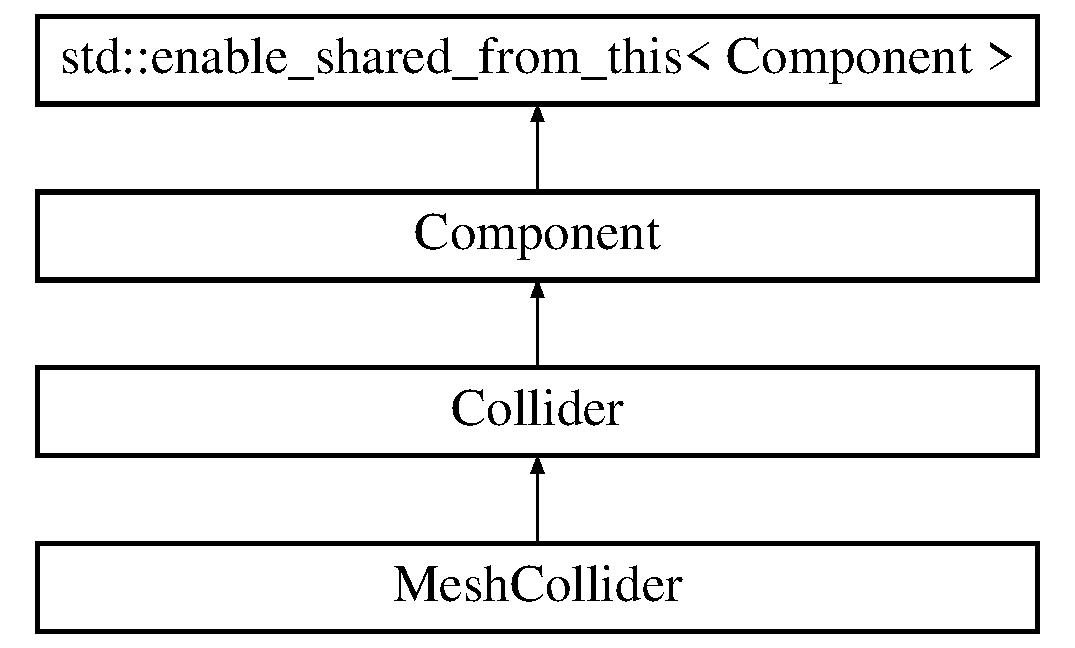
\includegraphics[height=4.000000cm]{class_mesh_collider}
\end{center}
\end{figure}
\subsection*{Public Member Functions}
\begin{DoxyCompactItemize}
\item 
\hyperlink{class_mesh_collider_ad7fdf5eb86b61c6edae3dfb48ea3ea03}{Mesh\+Collider} ()
\item 
virtual \hyperlink{class_mesh_collider_a1f026b06c7241d4f96e4bb2c6cc4fcc7}{$\sim$\+Mesh\+Collider} ()
\item 
virtual void \hyperlink{class_mesh_collider_ac906075dfa0f6ea801d82738c4b09231}{init} ()
\item 
virtual void \hyperlink{class_mesh_collider_a3d68ab01f24a654638319600ac720d57}{tick} (float delta\+Seconds) override
\item 
virtual shared\+\_\+ptr$<$ \hyperlink{class_component}{Component} $>$ \hyperlink{class_mesh_collider_a9965a490a1e945858dd9f1601b239878}{clone} () override
\item 
virtual shared\+\_\+ptr$<$ \hyperlink{class_component_description}{Component\+Description} $>$ \hyperlink{group__serialization__functions_ga92153fe80d9c2dcc91ce36050992f1d9}{get\+Component\+Description} () override
\item 
virtual void \hyperlink{group__serialization__functions_ga668f25c331d9519dfbd5f51a300cbb13}{deserialize} (shared\+\_\+ptr$<$ \hyperlink{class_component_description}{Component\+Description} $>$ desc) override
\end{DoxyCompactItemize}
\subsection*{Additional Inherited Members}


\subsection{Detailed Description}
\hyperlink{class_box_collider}{Box\+Collider} uses a \hyperlink{class_mesh}{Mesh} as the volume collider. Can either be real physics simulated or trigger only. 

\subsection{Constructor \& Destructor Documentation}
\hypertarget{class_mesh_collider_ad7fdf5eb86b61c6edae3dfb48ea3ea03}{}\index{Mesh\+Collider@{Mesh\+Collider}!Mesh\+Collider@{Mesh\+Collider}}
\index{Mesh\+Collider@{Mesh\+Collider}!Mesh\+Collider@{Mesh\+Collider}}
\subsubsection[{Mesh\+Collider()}]{\setlength{\rightskip}{0pt plus 5cm}Mesh\+Collider\+::\+Mesh\+Collider (
\begin{DoxyParamCaption}
{}
\end{DoxyParamCaption}
)}\label{class_mesh_collider_ad7fdf5eb86b61c6edae3dfb48ea3ea03}
Default Constructor \hypertarget{class_mesh_collider_a1f026b06c7241d4f96e4bb2c6cc4fcc7}{}\index{Mesh\+Collider@{Mesh\+Collider}!````~Mesh\+Collider@{$\sim$\+Mesh\+Collider}}
\index{````~Mesh\+Collider@{$\sim$\+Mesh\+Collider}!Mesh\+Collider@{Mesh\+Collider}}
\subsubsection[{$\sim$\+Mesh\+Collider()}]{\setlength{\rightskip}{0pt plus 5cm}Mesh\+Collider\+::$\sim$\+Mesh\+Collider (
\begin{DoxyParamCaption}
{}
\end{DoxyParamCaption}
)\hspace{0.3cm}{\ttfamily [virtual]}}\label{class_mesh_collider_a1f026b06c7241d4f96e4bb2c6cc4fcc7}
Default Destructor. Virtual because inherits from \hyperlink{class_collider}{Collider} 

\subsection{Member Function Documentation}
\hypertarget{class_mesh_collider_a9965a490a1e945858dd9f1601b239878}{}\index{Mesh\+Collider@{Mesh\+Collider}!clone@{clone}}
\index{clone@{clone}!Mesh\+Collider@{Mesh\+Collider}}
\subsubsection[{clone() override}]{\setlength{\rightskip}{0pt plus 5cm}shared\+\_\+ptr$<$ {\bf Component} $>$ Mesh\+Collider\+::clone (
\begin{DoxyParamCaption}
{}
\end{DoxyParamCaption}
)\hspace{0.3cm}{\ttfamily [override]}, {\ttfamily [virtual]}}\label{class_mesh_collider_a9965a490a1e945858dd9f1601b239878}
Clones current component (Prototype Design Pattern) \begin{DoxyReturn}{Returns}
shared\+\_\+ptr to cloned \hyperlink{class_mesh_collider}{Mesh\+Collider} \hyperlink{class_component}{Component} 
\end{DoxyReturn}


Implements \hyperlink{class_collider_a28d0829db9804b27590afc9979e61a1c}{Collider}.

\hypertarget{class_mesh_collider_ac906075dfa0f6ea801d82738c4b09231}{}\index{Mesh\+Collider@{Mesh\+Collider}!init@{init}}
\index{init@{init}!Mesh\+Collider@{Mesh\+Collider}}
\subsubsection[{init()}]{\setlength{\rightskip}{0pt plus 5cm}void Mesh\+Collider\+::init (
\begin{DoxyParamCaption}
{}
\end{DoxyParamCaption}
)\hspace{0.3cm}{\ttfamily [virtual]}}\label{class_mesh_collider_ac906075dfa0f6ea801d82738c4b09231}
Init component override. Create a new \hyperlink{class_mesh}{Mesh} Shape in the Phys\+X scene. 

Reimplemented from \hyperlink{class_collider_aed04ad82be15bcba1d3dc6a09f76dae6}{Collider}.

\hypertarget{class_mesh_collider_a3d68ab01f24a654638319600ac720d57}{}\index{Mesh\+Collider@{Mesh\+Collider}!tick@{tick}}
\index{tick@{tick}!Mesh\+Collider@{Mesh\+Collider}}
\subsubsection[{tick(float delta\+Seconds) override}]{\setlength{\rightskip}{0pt plus 5cm}void Mesh\+Collider\+::tick (
\begin{DoxyParamCaption}
\item[{float}]{delta\+Seconds}
\end{DoxyParamCaption}
)\hspace{0.3cm}{\ttfamily [override]}, {\ttfamily [virtual]}}\label{class_mesh_collider_a3d68ab01f24a654638319600ac720d57}
\hyperlink{class_component}{Component} tick override. Updates the scale of the \hyperlink{class_mesh}{Mesh} Shape in the Phys\+X scene. 

Reimplemented from \hyperlink{class_component_a72d67b02e6733c1a6fb73cbaaf8ebff4}{Component}.



The documentation for this class was generated from the following files\+:\begin{DoxyCompactItemize}
\item 
/\+Users/guilherme\+\_\+cunha/\+Dev/\+G\+I\+T\+H\+U\+B/\+G\+U\+Inity/\+Source/Mesh\+Collider.\+hpp\item 
/\+Users/guilherme\+\_\+cunha/\+Dev/\+G\+I\+T\+H\+U\+B/\+G\+U\+Inity/\+Source/Mesh\+Collider.\+cpp\end{DoxyCompactItemize}

\hypertarget{class_mesh_component}{}\section{Mesh\+Component Class Reference}
\label{class_mesh_component}\index{Mesh\+Component@{Mesh\+Component}}


{\ttfamily \#include $<$Mesh\+Component.\+hpp$>$}

Inheritance diagram for Mesh\+Component\+:\begin{figure}[H]
\begin{center}
\leavevmode
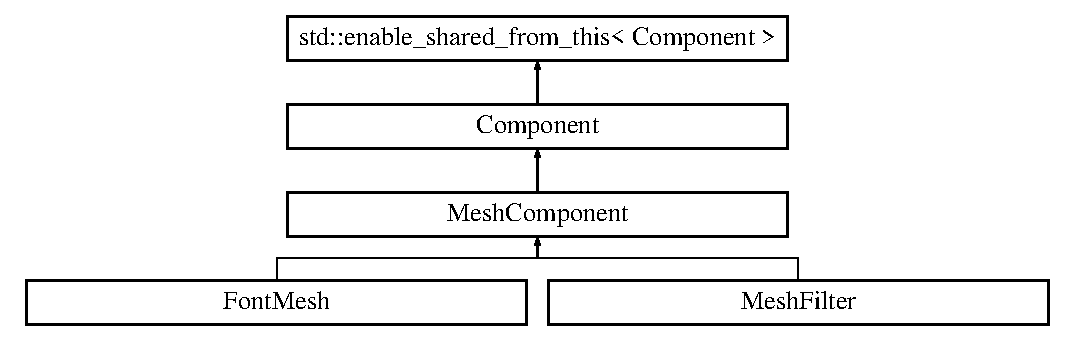
\includegraphics[height=4.000000cm]{class_mesh_component}
\end{center}
\end{figure}
\subsection*{Public Member Functions}
\begin{DoxyCompactItemize}
\item 
\hyperlink{class_mesh_component_a6f23f9f4c0fb23ee33a3798708c9a741}{Mesh\+Component} ()
\item 
virtual \hyperlink{class_mesh_component_a14f087d42e725d37d2414c7f32ca941a}{$\sim$\+Mesh\+Component} ()
\item 
void \hyperlink{class_mesh_component_a2971b2218704573c8bfc1e2ac0aa4fae}{set\+Mesh} (shared\+\_\+ptr$<$ \hyperlink{class_mesh}{Mesh} $>$ \hyperlink{class_mesh_component_ae985ae250fc6887e255e75f4c9a165dc}{mesh})
\item 
shared\+\_\+ptr$<$ \hyperlink{class_mesh}{Mesh} $>$ \hyperlink{class_mesh_component_a1388746fe37a996d6a17e4625ab0968a}{get\+Mesh} ()
\item 
void \hyperlink{class_mesh_component_a9d32173d75e3fa307cb53347e06bd325}{get\+Box\+Size} (shared\+\_\+ptr$<$ \hyperlink{class_actor}{Actor} $>$ actor, Px\+Vec3 \&box\+Size, Px\+Vec3 \&center)
\item 
void \hyperlink{class_mesh_component_a2dc1677ff14f5af49ec20bcaa84799b0}{get\+Sphere\+Size} (shared\+\_\+ptr$<$ \hyperlink{class_actor}{Actor} $>$ actor, float \&radius, Px\+Vec3 \&center)
\item 
void \hyperlink{class_mesh_component_acb19dbc4dfc54a99aa55538155cc459d}{get\+Capsule\+Geometry} (shared\+\_\+ptr$<$ \hyperlink{class_actor}{Actor} $>$actor, float \&radius, float \&half\+Height, Rotate\+Axis \&orientation, Px\+Vec3 \&center)
\item 
virtual shared\+\_\+ptr$<$ \hyperlink{class_component}{Component} $>$ \hyperlink{class_mesh_component_ace2f1acdce65f1c37b56a5b3ef507e8d}{clone} ()=0
\item 
virtual shared\+\_\+ptr$<$ \hyperlink{class_component_description}{Component\+Description} $>$ \hyperlink{group__serialization__functions_ga10950983c0abed7fc5381383e211904f}{get\+Component\+Description} () override
\item 
virtual void \hyperlink{group__serialization__functions_gac2630e3fbb6a7eeb6b2f6d40e2a67bfa}{deserialize} (shared\+\_\+ptr$<$ \hyperlink{class_component_description}{Component\+Description} $>$ desc) override
\end{DoxyCompactItemize}
\subsection*{Protected Attributes}
\begin{DoxyCompactItemize}
\item 
shared\+\_\+ptr$<$ \hyperlink{class_mesh}{Mesh} $>$ \hyperlink{class_mesh_component_ae985ae250fc6887e255e75f4c9a165dc}{mesh}
\end{DoxyCompactItemize}
\subsection*{Additional Inherited Members}


\subsection{Detailed Description}
\hyperlink{class_mesh_component}{Mesh\+Component} is a \hyperlink{class_component}{Component} makes a reference to a \hyperlink{class_mesh}{Mesh} asset. This is important to prevent the same \hyperlink{class_mesh}{Mesh} to live multiple times in memory. This class is inherited used by \hyperlink{class_mesh_filter}{Mesh\+Filter} and \hyperlink{class_font_mesh}{Font\+Mesh} 

\subsection{Constructor \& Destructor Documentation}
\hypertarget{class_mesh_component_a6f23f9f4c0fb23ee33a3798708c9a741}{}\index{Mesh\+Component@{Mesh\+Component}!Mesh\+Component@{Mesh\+Component}}
\index{Mesh\+Component@{Mesh\+Component}!Mesh\+Component@{Mesh\+Component}}
\subsubsection[{Mesh\+Component()}]{\setlength{\rightskip}{0pt plus 5cm}Mesh\+Component\+::\+Mesh\+Component (
\begin{DoxyParamCaption}
{}
\end{DoxyParamCaption}
)}\label{class_mesh_component_a6f23f9f4c0fb23ee33a3798708c9a741}
Default Constructor \hypertarget{class_mesh_component_a14f087d42e725d37d2414c7f32ca941a}{}\index{Mesh\+Component@{Mesh\+Component}!````~Mesh\+Component@{$\sim$\+Mesh\+Component}}
\index{````~Mesh\+Component@{$\sim$\+Mesh\+Component}!Mesh\+Component@{Mesh\+Component}}
\subsubsection[{$\sim$\+Mesh\+Component()}]{\setlength{\rightskip}{0pt plus 5cm}Mesh\+Component\+::$\sim$\+Mesh\+Component (
\begin{DoxyParamCaption}
{}
\end{DoxyParamCaption}
)\hspace{0.3cm}{\ttfamily [virtual]}}\label{class_mesh_component_a14f087d42e725d37d2414c7f32ca941a}
Default Destructor. Virtual because this is a parent class 

\subsection{Member Function Documentation}
\hypertarget{class_mesh_component_ace2f1acdce65f1c37b56a5b3ef507e8d}{}\index{Mesh\+Component@{Mesh\+Component}!clone@{clone}}
\index{clone@{clone}!Mesh\+Component@{Mesh\+Component}}
\subsubsection[{clone()=0}]{\setlength{\rightskip}{0pt plus 5cm}virtual shared\+\_\+ptr$<${\bf Component}$>$ Mesh\+Component\+::clone (
\begin{DoxyParamCaption}
{}
\end{DoxyParamCaption}
)\hspace{0.3cm}{\ttfamily [pure virtual]}}\label{class_mesh_component_ace2f1acdce65f1c37b56a5b3ef507e8d}
Pure virtual function. Clones current component (Prototype Design Pattern) \begin{DoxyReturn}{Returns}
shared\+\_\+ptr to cloned \hyperlink{class_mesh_component}{Mesh\+Component} \hyperlink{class_component}{Component} 
\end{DoxyReturn}


Implements \hyperlink{class_component_a74c984bd819bbef16fd4f306a90d34fe}{Component}.



Implemented in \hyperlink{class_font_mesh_a4dd3900fcbb33aca326d1cd1871e7b92}{Font\+Mesh}, and \hyperlink{class_mesh_filter_a6645cf7989fad04e40096955296b96a2}{Mesh\+Filter}.

\hypertarget{class_mesh_component_a9d32173d75e3fa307cb53347e06bd325}{}\index{Mesh\+Component@{Mesh\+Component}!get\+Box\+Size@{get\+Box\+Size}}
\index{get\+Box\+Size@{get\+Box\+Size}!Mesh\+Component@{Mesh\+Component}}
\subsubsection[{get\+Box\+Size(shared\+\_\+ptr$<$ Actor $>$ actor, Px\+Vec3 \&box\+Size, Px\+Vec3 \&center)}]{\setlength{\rightskip}{0pt plus 5cm}void Mesh\+Component\+::get\+Box\+Size (
\begin{DoxyParamCaption}
\item[{shared\+\_\+ptr$<$ {\bf Actor} $>$}]{actor, }
\item[{Px\+Vec3 \&}]{box\+Size, }
\item[{Px\+Vec3 \&}]{center}
\end{DoxyParamCaption}
)}\label{class_mesh_component_a9d32173d75e3fa307cb53347e06bd325}
Gets the center and the A\+A\+B\+B size for the \hyperlink{class_actor}{Actor} that this component is attached to \hypertarget{class_mesh_component_acb19dbc4dfc54a99aa55538155cc459d}{}\index{Mesh\+Component@{Mesh\+Component}!get\+Capsule\+Geometry@{get\+Capsule\+Geometry}}
\index{get\+Capsule\+Geometry@{get\+Capsule\+Geometry}!Mesh\+Component@{Mesh\+Component}}
\subsubsection[{get\+Capsule\+Geometry(shared\+\_\+ptr$<$ Actor $>$actor, float \&radius, float \&half\+Height, Rotate\+Axis \&orientation, Px\+Vec3 \&center)}]{\setlength{\rightskip}{0pt plus 5cm}void Mesh\+Component\+::get\+Capsule\+Geometry (
\begin{DoxyParamCaption}
\item[{shared\+\_\+ptr$<$ {\bf Actor} $>$}]{actor, }
\item[{float \&}]{radius, }
\item[{float \&}]{half\+Height, }
\item[{Rotate\+Axis \&}]{orientation, }
\item[{Px\+Vec3 \&}]{center}
\end{DoxyParamCaption}
)}\label{class_mesh_component_acb19dbc4dfc54a99aa55538155cc459d}
Gets the center and the capsule description for the \hyperlink{class_actor}{Actor} that this component is attached to \hypertarget{class_mesh_component_a1388746fe37a996d6a17e4625ab0968a}{}\index{Mesh\+Component@{Mesh\+Component}!get\+Mesh@{get\+Mesh}}
\index{get\+Mesh@{get\+Mesh}!Mesh\+Component@{Mesh\+Component}}
\subsubsection[{get\+Mesh()}]{\setlength{\rightskip}{0pt plus 5cm}shared\+\_\+ptr$<$ {\bf Mesh} $>$ Mesh\+Component\+::get\+Mesh (
\begin{DoxyParamCaption}
{}
\end{DoxyParamCaption}
)}\label{class_mesh_component_a1388746fe37a996d6a17e4625ab0968a}
mesh Setter

mesh Getter \hypertarget{class_mesh_component_a2dc1677ff14f5af49ec20bcaa84799b0}{}\index{Mesh\+Component@{Mesh\+Component}!get\+Sphere\+Size@{get\+Sphere\+Size}}
\index{get\+Sphere\+Size@{get\+Sphere\+Size}!Mesh\+Component@{Mesh\+Component}}
\subsubsection[{get\+Sphere\+Size(shared\+\_\+ptr$<$ Actor $>$ actor, float \&radius, Px\+Vec3 \&center)}]{\setlength{\rightskip}{0pt plus 5cm}void Mesh\+Component\+::get\+Sphere\+Size (
\begin{DoxyParamCaption}
\item[{shared\+\_\+ptr$<$ {\bf Actor} $>$}]{actor, }
\item[{float \&}]{radius, }
\item[{Px\+Vec3 \&}]{center}
\end{DoxyParamCaption}
)}\label{class_mesh_component_a2dc1677ff14f5af49ec20bcaa84799b0}
Gets the center and the radius for the \hyperlink{class_actor}{Actor} that this component is attached to \hypertarget{class_mesh_component_a2971b2218704573c8bfc1e2ac0aa4fae}{}\index{Mesh\+Component@{Mesh\+Component}!set\+Mesh@{set\+Mesh}}
\index{set\+Mesh@{set\+Mesh}!Mesh\+Component@{Mesh\+Component}}
\subsubsection[{set\+Mesh(shared\+\_\+ptr$<$ Mesh $>$ mesh)}]{\setlength{\rightskip}{0pt plus 5cm}void Mesh\+Component\+::set\+Mesh (
\begin{DoxyParamCaption}
\item[{shared\+\_\+ptr$<$ {\bf Mesh} $>$}]{mesh}
\end{DoxyParamCaption}
)}\label{class_mesh_component_a2971b2218704573c8bfc1e2ac0aa4fae}
mesh Getter

mesh Setter 

\subsection{Member Data Documentation}
\hypertarget{class_mesh_component_ae985ae250fc6887e255e75f4c9a165dc}{}\index{Mesh\+Component@{Mesh\+Component}!mesh@{mesh}}
\index{mesh@{mesh}!Mesh\+Component@{Mesh\+Component}}
\subsubsection[{mesh}]{\setlength{\rightskip}{0pt plus 5cm}shared\+\_\+ptr$<${\bf Mesh}$>$ Mesh\+Component\+::mesh\hspace{0.3cm}{\ttfamily [protected]}}\label{class_mesh_component_ae985ae250fc6887e255e75f4c9a165dc}
The \hyperlink{class_mesh}{Mesh} \hyperlink{class_asset}{Asset} 

The documentation for this class was generated from the following files\+:\begin{DoxyCompactItemize}
\item 
/\+Users/guilherme\+\_\+cunha/\+Dev/\+G\+I\+T\+H\+U\+B/\+G\+U\+Inity/\+Source/Mesh\+Component.\+hpp\item 
/\+Users/guilherme\+\_\+cunha/\+Dev/\+G\+I\+T\+H\+U\+B/\+G\+U\+Inity/\+Source/Mesh\+Component.\+cpp\end{DoxyCompactItemize}

\hypertarget{class_mesh_filter}{}\section{Mesh\+Filter Class Reference}
\label{class_mesh_filter}\index{Mesh\+Filter@{Mesh\+Filter}}


{\ttfamily \#include $<$Mesh\+Filter.\+hpp$>$}

Inheritance diagram for Mesh\+Filter\+:\begin{figure}[H]
\begin{center}
\leavevmode
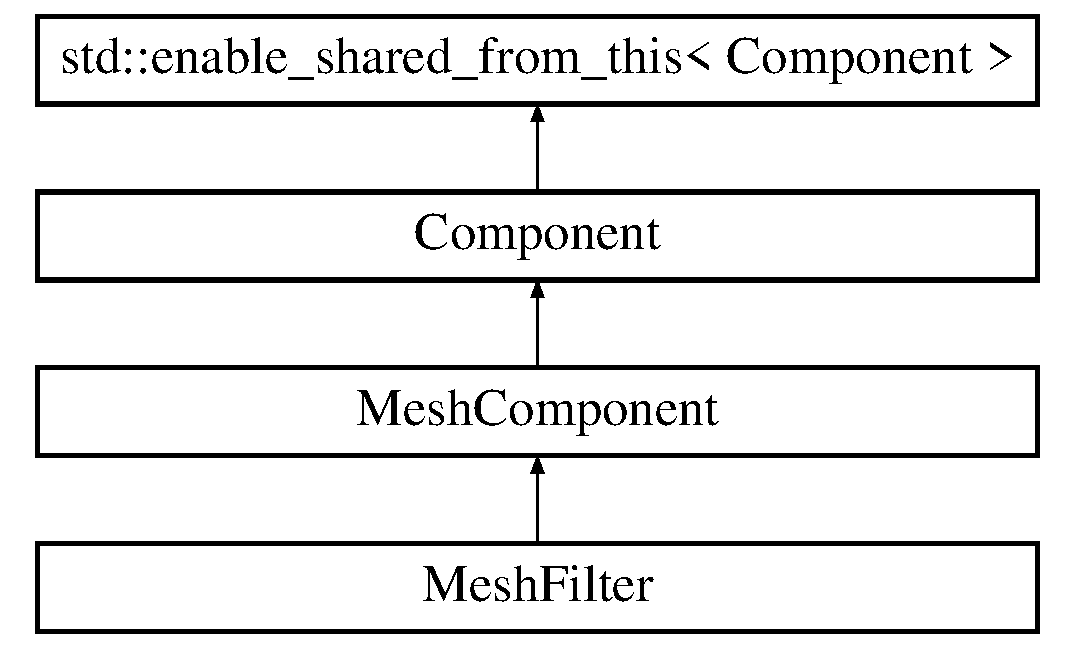
\includegraphics[height=4.000000cm]{class_mesh_filter}
\end{center}
\end{figure}
\subsection*{Public Member Functions}
\begin{DoxyCompactItemize}
\item 
\hyperlink{class_mesh_filter_aad0010eab8429ee8a574f6c1d57126e6}{Mesh\+Filter} ()
\item 
virtual \hyperlink{class_mesh_filter_a8ffe38518dd8010150201f70789048b4}{$\sim$\+Mesh\+Filter} ()
\item 
virtual shared\+\_\+ptr$<$ \hyperlink{class_component}{Component} $>$ \hyperlink{class_mesh_filter_a6645cf7989fad04e40096955296b96a2}{clone} () override
\item 
virtual shared\+\_\+ptr$<$ \hyperlink{class_component_description}{Component\+Description} $>$ \hyperlink{group__serialization__functions_ga3f175929ed6c3d53b330eca5de9c5a13}{get\+Component\+Description} () override
\item 
virtual void \hyperlink{group__serialization__functions_gae0449262f3398c229e95911f69930acb}{deserialize} (shared\+\_\+ptr$<$ \hyperlink{class_component_description}{Component\+Description} $>$ desc) override
\end{DoxyCompactItemize}
\subsection*{Additional Inherited Members}


\subsection{Detailed Description}
\hyperlink{class_mesh_filter}{Mesh\+Filter} makes reference to a \hyperlink{class_mesh}{Mesh}. It\textquotesingle{}s used in combination with \hyperlink{class_mesh_renderer}{Mesh\+Renderer} to render a \hyperlink{class_mesh}{Mesh} on screen 

\subsection{Constructor \& Destructor Documentation}
\hypertarget{class_mesh_filter_aad0010eab8429ee8a574f6c1d57126e6}{}\index{Mesh\+Filter@{Mesh\+Filter}!Mesh\+Filter@{Mesh\+Filter}}
\index{Mesh\+Filter@{Mesh\+Filter}!Mesh\+Filter@{Mesh\+Filter}}
\subsubsection[{Mesh\+Filter()}]{\setlength{\rightskip}{0pt plus 5cm}Mesh\+Filter\+::\+Mesh\+Filter (
\begin{DoxyParamCaption}
{}
\end{DoxyParamCaption}
)}\label{class_mesh_filter_aad0010eab8429ee8a574f6c1d57126e6}
Default Constructor \hypertarget{class_mesh_filter_a8ffe38518dd8010150201f70789048b4}{}\index{Mesh\+Filter@{Mesh\+Filter}!````~Mesh\+Filter@{$\sim$\+Mesh\+Filter}}
\index{````~Mesh\+Filter@{$\sim$\+Mesh\+Filter}!Mesh\+Filter@{Mesh\+Filter}}
\subsubsection[{$\sim$\+Mesh\+Filter()}]{\setlength{\rightskip}{0pt plus 5cm}Mesh\+Filter\+::$\sim$\+Mesh\+Filter (
\begin{DoxyParamCaption}
{}
\end{DoxyParamCaption}
)\hspace{0.3cm}{\ttfamily [virtual]}}\label{class_mesh_filter_a8ffe38518dd8010150201f70789048b4}
Default Destructor. Virtual because it\textquotesingle{}s child class. 

\subsection{Member Function Documentation}
\hypertarget{class_mesh_filter_a6645cf7989fad04e40096955296b96a2}{}\index{Mesh\+Filter@{Mesh\+Filter}!clone@{clone}}
\index{clone@{clone}!Mesh\+Filter@{Mesh\+Filter}}
\subsubsection[{clone() override}]{\setlength{\rightskip}{0pt plus 5cm}shared\+\_\+ptr$<$ {\bf Component} $>$ Mesh\+Filter\+::clone (
\begin{DoxyParamCaption}
{}
\end{DoxyParamCaption}
)\hspace{0.3cm}{\ttfamily [override]}, {\ttfamily [virtual]}}\label{class_mesh_filter_a6645cf7989fad04e40096955296b96a2}
Clones current component (Prototype Design Pattern) \begin{DoxyReturn}{Returns}
shared\+\_\+ptr to cloned \hyperlink{class_mesh_filter}{Mesh\+Filter} \hyperlink{class_component}{Component} 
\end{DoxyReturn}


Implements \hyperlink{class_mesh_component_ace2f1acdce65f1c37b56a5b3ef507e8d}{Mesh\+Component}.



The documentation for this class was generated from the following files\+:\begin{DoxyCompactItemize}
\item 
/\+Users/guilherme\+\_\+cunha/\+Dev/\+G\+I\+T\+H\+U\+B/\+G\+U\+Inity/\+Source/Mesh\+Filter.\+hpp\item 
/\+Users/guilherme\+\_\+cunha/\+Dev/\+G\+I\+T\+H\+U\+B/\+G\+U\+Inity/\+Source/Mesh\+Filter.\+cpp\end{DoxyCompactItemize}

\hypertarget{class_mesh_filter_description}{}\section{Mesh\+Filter\+Description Class Reference}
\label{class_mesh_filter_description}\index{Mesh\+Filter\+Description@{Mesh\+Filter\+Description}}
Inheritance diagram for Mesh\+Filter\+Description\+:\begin{figure}[H]
\begin{center}
\leavevmode
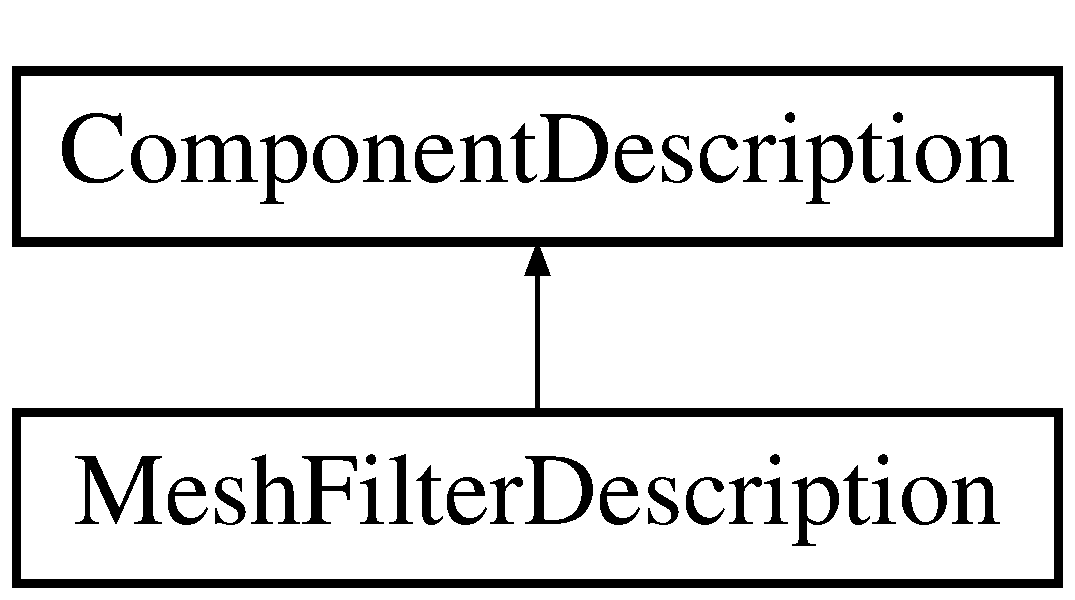
\includegraphics[height=2.000000cm]{class_mesh_filter_description}
\end{center}
\end{figure}
\subsection*{Public Member Functions}
\begin{DoxyCompactItemize}
\item 
\hypertarget{class_mesh_filter_description_a8ab678722bd880505fa05fcc1b0f8694}{}{\bfseries Mesh\+Filter\+Description} (int id)\label{class_mesh_filter_description_a8ab678722bd880505fa05fcc1b0f8694}

\end{DoxyCompactItemize}
\subsection*{Public Attributes}
\begin{DoxyCompactItemize}
\item 
\hypertarget{class_mesh_filter_description_aacb950a39abb1be259dca00654bf3893}{}int {\bfseries mesh\+I\+D}\label{class_mesh_filter_description_aacb950a39abb1be259dca00654bf3893}

\end{DoxyCompactItemize}


The documentation for this class was generated from the following file\+:\begin{DoxyCompactItemize}
\item 
/\+Users/guilherme\+\_\+cunha/\+Dev/\+G\+I\+T\+H\+U\+B/\+G\+U\+Inity/\+Source/Serialization\+Structs.\+hpp\end{DoxyCompactItemize}

\hypertarget{class_mesh_importer}{}\section{Mesh\+Importer Class Reference}
\label{class_mesh_importer}\index{Mesh\+Importer@{Mesh\+Importer}}
\subsection*{Public Member Functions}
\begin{DoxyCompactItemize}
\item 
\hypertarget{class_mesh_importer_ab2796aabebc5918c76569b3a644713d7}{}void {\bfseries init} ()\label{class_mesh_importer_ab2796aabebc5918c76569b3a644713d7}

\item 
\hypertarget{class_mesh_importer_a22b8d0d5334546680688976059dc6580}{}void {\bfseries shutdown} ()\label{class_mesh_importer_a22b8d0d5334546680688976059dc6580}

\item 
\hypertarget{class_mesh_importer_ad045f72cce53c45688ac84999698204a}{}shared\+\_\+ptr$<$ \hyperlink{class_mesh}{Mesh} $>$ {\bfseries import\+Fbx\+Mesh} (string filename)\label{class_mesh_importer_ad045f72cce53c45688ac84999698204a}

\item 
\hypertarget{class_mesh_importer_a9dc165f78e1b759ee6058eff5968c615}{}void {\bfseries import\+Fbx\+Skeleton} (Fbx\+Skeleton $\ast$skeleton\+Node)\label{class_mesh_importer_a9dc165f78e1b759ee6058eff5968c615}

\item 
\hypertarget{class_mesh_importer_af2231e344407382855918313611fb43e}{}void {\bfseries import\+Fbx\+Skin} (Fbx\+Skin $\ast$skin\+Node)\label{class_mesh_importer_af2231e344407382855918313611fb43e}

\item 
\hypertarget{class_mesh_importer_aaf12107c1df43dce0108802245543f40}{}shared\+\_\+ptr$<$ \hyperlink{class_mesh}{Mesh} $>$ {\bfseries import\+Fbx\+Mesh} (Fbx\+Scene $\ast$scene, Fbx\+Mesh $\ast$mesh\+Node)\label{class_mesh_importer_aaf12107c1df43dce0108802245543f40}

\item 
\hypertarget{class_mesh_importer_aa0acb8ba390c4a30c5c60c97c24c981e}{}shared\+\_\+ptr$<$ \hyperlink{class_skinned_mesh}{Skinned\+Mesh} $>$ {\bfseries import\+Fbx\+Skinned\+Mesh} (Fbx\+Scene $\ast$scene, Fbx\+Mesh $\ast$mesh\+Node)\label{class_mesh_importer_aa0acb8ba390c4a30c5c60c97c24c981e}

\item 
\hypertarget{class_mesh_importer_a16f2e17c0789d1ba30c82c54631d6c54}{}void {\bfseries import\+Fbx\+Animation} (Fbx\+Scene $\ast$scene, Fbx\+Node $\ast$node)\label{class_mesh_importer_a16f2e17c0789d1ba30c82c54631d6c54}

\item 
\hypertarget{class_mesh_importer_a2ee7226a821d06fb7b800e4d600ad781}{}shared\+\_\+ptr$<$ \hyperlink{class_mesh}{Mesh} $>$ {\bfseries import\+Obj\+Mesh} (string filename)\label{class_mesh_importer_a2ee7226a821d06fb7b800e4d600ad781}

\item 
\hypertarget{class_mesh_importer_afd1e9b2a4bbb695888073f5bbe01f70a}{}bool {\bfseries is\+Mesh\+Skinned} (Fbx\+Mesh $\ast$mesh\+Node)\label{class_mesh_importer_afd1e9b2a4bbb695888073f5bbe01f70a}

\item 
\hypertarget{class_mesh_importer_abde4c4f38e08ba95fbc292a43520b009}{}void {\bfseries get\+Vertex\+Data} (Fbx\+Mesh $\ast$m\+\_\+p\+Mesh, int u\+Poly, int u\+Vertex, Fbx\+Vector4 \&fbx\+Vertex, Fbx\+Vector4 \&fbx\+Normal, Fbx\+Vector2 \&fbx\+U\+V)\label{class_mesh_importer_abde4c4f38e08ba95fbc292a43520b009}

\item 
\hypertarget{class_mesh_importer_ae0bc798bf57d675b52a438777a561ea8}{}{\footnotesize template$<$typename T $>$ }\\bool {\bfseries find\+Vertex} (std\+::map$<$ T, unsigned short $>$ \&vertex\+Map, T \&v, unsigned short \&index)\label{class_mesh_importer_ae0bc798bf57d675b52a438777a561ea8}

\end{DoxyCompactItemize}
\subsection*{Public Attributes}
\begin{DoxyCompactItemize}
\item 
\hypertarget{class_mesh_importer_ae85eb3068f2e8f80fffa67e0b516d69c}{}Fbx\+Manager $\ast$ {\bfseries fbx\+Manager}\label{class_mesh_importer_ae85eb3068f2e8f80fffa67e0b516d69c}

\item 
\hypertarget{class_mesh_importer_aa78bacc0afc35c16656dabefed686c84}{}Fbx\+I\+O\+Settings $\ast$ {\bfseries ios}\label{class_mesh_importer_aa78bacc0afc35c16656dabefed686c84}

\item 
\hypertarget{class_mesh_importer_ad5d179f8f8c3f993c5779930775df83c}{}Fbx\+Importer $\ast$ {\bfseries l\+Importer}\label{class_mesh_importer_ad5d179f8f8c3f993c5779930775df83c}

\end{DoxyCompactItemize}


The documentation for this class was generated from the following files\+:\begin{DoxyCompactItemize}
\item 
/\+Users/guilherme\+\_\+cunha/\+Dev/\+G\+I\+T\+H\+U\+B/\+G\+U\+Inity/\+Source/Mesh\+Importer.\+hpp\item 
/\+Users/guilherme\+\_\+cunha/\+Dev/\+G\+I\+T\+H\+U\+B/\+G\+U\+Inity/\+Source/Mesh\+Importer.\+cpp\end{DoxyCompactItemize}

\hypertarget{class_mesh_renderer}{}\section{Mesh\+Renderer Class Reference}
\label{class_mesh_renderer}\index{Mesh\+Renderer@{Mesh\+Renderer}}
Inheritance diagram for Mesh\+Renderer\+:\begin{figure}[H]
\begin{center}
\leavevmode
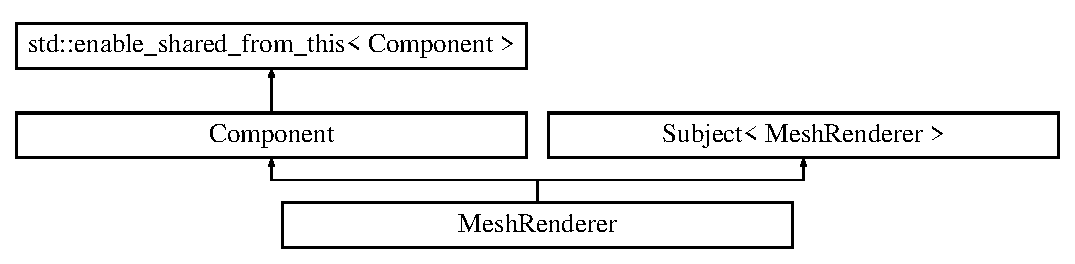
\includegraphics[height=3.000000cm]{class_mesh_renderer}
\end{center}
\end{figure}
\subsection*{Public Member Functions}
\begin{DoxyCompactItemize}
\item 
\hyperlink{class_mesh_renderer_aa928cebc7dc3602f61bf676761476fb2}{Mesh\+Renderer} ()
\item 
virtual \hyperlink{class_mesh_renderer_aeae128e155e478309aa8fd434abc7892}{$\sim$\+Mesh\+Renderer} ()
\item 
void \hyperlink{class_mesh_renderer_a7680dd341fa2b5ad4b31e9d3c25918f3}{set\+Material} (shared\+\_\+ptr$<$ \hyperlink{class_material}{Material} $>$ material)
\item 
shared\+\_\+ptr$<$ \hyperlink{class_material}{Material} $>$ \hyperlink{class_mesh_renderer_ab9c30678cf66a6fb3b8de32ab03c6a0b}{get\+Material} ()
\item 
void \hyperlink{class_mesh_renderer_ac750721941d7615e7443f459d04c5c60}{set\+Mesh\+Component} (shared\+\_\+ptr$<$ \hyperlink{class_mesh_component}{Mesh\+Component} $>$ mesh)
\item 
shared\+\_\+ptr$<$ \hyperlink{class_mesh_component}{Mesh\+Component} $>$ \hyperlink{class_mesh_renderer_a395bef0a7ce1b5f8973ac690fd7f1b2c}{get\+Mesh\+Component} ()
\item 
virtual void \hyperlink{class_mesh_renderer_ae77ac8e3b28e1890771860d5726fe043}{init} () override
\item 
virtual void \hyperlink{class_mesh_renderer_acb0c4dc40c30d70157adb51612e08013}{destroy} () override
\item 
virtual shared\+\_\+ptr$<$ \hyperlink{class_component}{Component} $>$ \hyperlink{class_mesh_renderer_a78a5a5b66bb12c2b50f5356292afd93a}{clone} () override
\item 
virtual shared\+\_\+ptr$<$ \hyperlink{class_component_description}{Component\+Description} $>$ \hyperlink{group__serialization__functions_gaf9b3799dcfb2bc87f5ce21c34c9fbaff}{get\+Component\+Description} () override
\item 
virtual void \hyperlink{group__serialization__functions_ga210ca500925eeb32174581ef37ea5b59}{deserialize} (shared\+\_\+ptr$<$ \hyperlink{class_component_description}{Component\+Description} $>$ desc) override
\end{DoxyCompactItemize}
\subsection*{Additional Inherited Members}


\subsection{Constructor \& Destructor Documentation}
\hypertarget{class_mesh_renderer_aa928cebc7dc3602f61bf676761476fb2}{}\index{Mesh\+Renderer@{Mesh\+Renderer}!Mesh\+Renderer@{Mesh\+Renderer}}
\index{Mesh\+Renderer@{Mesh\+Renderer}!Mesh\+Renderer@{Mesh\+Renderer}}
\subsubsection[{Mesh\+Renderer()}]{\setlength{\rightskip}{0pt plus 5cm}Mesh\+Renderer\+::\+Mesh\+Renderer (
\begin{DoxyParamCaption}
{}
\end{DoxyParamCaption}
)}\label{class_mesh_renderer_aa928cebc7dc3602f61bf676761476fb2}
Default Constructor \hypertarget{class_mesh_renderer_aeae128e155e478309aa8fd434abc7892}{}\index{Mesh\+Renderer@{Mesh\+Renderer}!````~Mesh\+Renderer@{$\sim$\+Mesh\+Renderer}}
\index{````~Mesh\+Renderer@{$\sim$\+Mesh\+Renderer}!Mesh\+Renderer@{Mesh\+Renderer}}
\subsubsection[{$\sim$\+Mesh\+Renderer()}]{\setlength{\rightskip}{0pt plus 5cm}Mesh\+Renderer\+::$\sim$\+Mesh\+Renderer (
\begin{DoxyParamCaption}
{}
\end{DoxyParamCaption}
)\hspace{0.3cm}{\ttfamily [virtual]}}\label{class_mesh_renderer_aeae128e155e478309aa8fd434abc7892}
Default Destructor. Virtual cause it\textquotesingle{}s child class 

\subsection{Member Function Documentation}
\hypertarget{class_mesh_renderer_a78a5a5b66bb12c2b50f5356292afd93a}{}\index{Mesh\+Renderer@{Mesh\+Renderer}!clone@{clone}}
\index{clone@{clone}!Mesh\+Renderer@{Mesh\+Renderer}}
\subsubsection[{clone() override}]{\setlength{\rightskip}{0pt plus 5cm}shared\+\_\+ptr$<$ {\bf Component} $>$ Mesh\+Renderer\+::clone (
\begin{DoxyParamCaption}
{}
\end{DoxyParamCaption}
)\hspace{0.3cm}{\ttfamily [override]}, {\ttfamily [virtual]}}\label{class_mesh_renderer_a78a5a5b66bb12c2b50f5356292afd93a}
Clones current component (Prototype Design Pattern) \begin{DoxyReturn}{Returns}
shared\+\_\+ptr to cloned \hyperlink{class_mesh_renderer}{Mesh\+Renderer} \hyperlink{class_component}{Component} 
\end{DoxyReturn}


Implements \hyperlink{class_component_a74c984bd819bbef16fd4f306a90d34fe}{Component}.

\hypertarget{class_mesh_renderer_acb0c4dc40c30d70157adb51612e08013}{}\index{Mesh\+Renderer@{Mesh\+Renderer}!destroy@{destroy}}
\index{destroy@{destroy}!Mesh\+Renderer@{Mesh\+Renderer}}
\subsubsection[{destroy() override}]{\setlength{\rightskip}{0pt plus 5cm}void Mesh\+Renderer\+::destroy (
\begin{DoxyParamCaption}
{}
\end{DoxyParamCaption}
)\hspace{0.3cm}{\ttfamily [override]}, {\ttfamily [virtual]}}\label{class_mesh_renderer_acb0c4dc40c30d70157adb51612e08013}
\hyperlink{class_component}{Component} destroy. Notifies this \hyperlink{class_mesh_renderer}{Mesh\+Renderer} has been destroyed 

Reimplemented from \hyperlink{class_component_a77b8fff56ddce5dd0b4a9dabb0b5202b}{Component}.

\hypertarget{class_mesh_renderer_ab9c30678cf66a6fb3b8de32ab03c6a0b}{}\index{Mesh\+Renderer@{Mesh\+Renderer}!get\+Material@{get\+Material}}
\index{get\+Material@{get\+Material}!Mesh\+Renderer@{Mesh\+Renderer}}
\subsubsection[{get\+Material()}]{\setlength{\rightskip}{0pt plus 5cm}shared\+\_\+ptr$<$ {\bf Material} $>$ Mesh\+Renderer\+::get\+Material (
\begin{DoxyParamCaption}
{}
\end{DoxyParamCaption}
)}\label{class_mesh_renderer_ab9c30678cf66a6fb3b8de32ab03c6a0b}
material getter \hypertarget{class_mesh_renderer_a395bef0a7ce1b5f8973ac690fd7f1b2c}{}\index{Mesh\+Renderer@{Mesh\+Renderer}!get\+Mesh\+Component@{get\+Mesh\+Component}}
\index{get\+Mesh\+Component@{get\+Mesh\+Component}!Mesh\+Renderer@{Mesh\+Renderer}}
\subsubsection[{get\+Mesh\+Component()}]{\setlength{\rightskip}{0pt plus 5cm}shared\+\_\+ptr$<$ {\bf Mesh\+Component} $>$ Mesh\+Renderer\+::get\+Mesh\+Component (
\begin{DoxyParamCaption}
{}
\end{DoxyParamCaption}
)}\label{class_mesh_renderer_a395bef0a7ce1b5f8973ac690fd7f1b2c}
mesh\+Component getter \hypertarget{class_mesh_renderer_ae77ac8e3b28e1890771860d5726fe043}{}\index{Mesh\+Renderer@{Mesh\+Renderer}!init@{init}}
\index{init@{init}!Mesh\+Renderer@{Mesh\+Renderer}}
\subsubsection[{init() override}]{\setlength{\rightskip}{0pt plus 5cm}void Mesh\+Renderer\+::init (
\begin{DoxyParamCaption}
{}
\end{DoxyParamCaption}
)\hspace{0.3cm}{\ttfamily [override]}, {\ttfamily [virtual]}}\label{class_mesh_renderer_ae77ac8e3b28e1890771860d5726fe043}
\hyperlink{class_component}{Component} init override. Tries to get a \hyperlink{class_mesh_component}{Mesh\+Component} from the owner \hyperlink{class_actor}{Actor} and notifies that a new \hyperlink{class_mesh_renderer}{Mesh\+Renderer} has been created 

Reimplemented from \hyperlink{class_component_a162f8cdc070537a71f2ad0b5e763b86f}{Component}.

\hypertarget{class_mesh_renderer_a7680dd341fa2b5ad4b31e9d3c25918f3}{}\index{Mesh\+Renderer@{Mesh\+Renderer}!set\+Material@{set\+Material}}
\index{set\+Material@{set\+Material}!Mesh\+Renderer@{Mesh\+Renderer}}
\subsubsection[{set\+Material(shared\+\_\+ptr$<$ Material $>$ material)}]{\setlength{\rightskip}{0pt plus 5cm}void Mesh\+Renderer\+::set\+Material (
\begin{DoxyParamCaption}
\item[{shared\+\_\+ptr$<$ {\bf Material} $>$}]{material}
\end{DoxyParamCaption}
)}\label{class_mesh_renderer_a7680dd341fa2b5ad4b31e9d3c25918f3}
material setter \hypertarget{class_mesh_renderer_ac750721941d7615e7443f459d04c5c60}{}\index{Mesh\+Renderer@{Mesh\+Renderer}!set\+Mesh\+Component@{set\+Mesh\+Component}}
\index{set\+Mesh\+Component@{set\+Mesh\+Component}!Mesh\+Renderer@{Mesh\+Renderer}}
\subsubsection[{set\+Mesh\+Component(shared\+\_\+ptr$<$ Mesh\+Component $>$ mesh)}]{\setlength{\rightskip}{0pt plus 5cm}void Mesh\+Renderer\+::set\+Mesh\+Component (
\begin{DoxyParamCaption}
\item[{shared\+\_\+ptr$<$ {\bf Mesh\+Component} $>$}]{mesh\+Component}
\end{DoxyParamCaption}
)}\label{class_mesh_renderer_ac750721941d7615e7443f459d04c5c60}
mesh\+Component setter 

The documentation for this class was generated from the following files\+:\begin{DoxyCompactItemize}
\item 
/\+Users/guilherme\+\_\+cunha/\+Dev/\+G\+I\+T\+H\+U\+B/\+G\+U\+Inity/\+Source/Mesh\+Renderer.\+hpp\item 
/\+Users/guilherme\+\_\+cunha/\+Dev/\+G\+I\+T\+H\+U\+B/\+G\+U\+Inity/\+Source/Mesh\+Renderer.\+cpp\end{DoxyCompactItemize}

\hypertarget{class_mesh_renderer_description}{}\section{Mesh\+Renderer\+Description Class Reference}
\label{class_mesh_renderer_description}\index{Mesh\+Renderer\+Description@{Mesh\+Renderer\+Description}}
Inheritance diagram for Mesh\+Renderer\+Description\+:\begin{figure}[H]
\begin{center}
\leavevmode
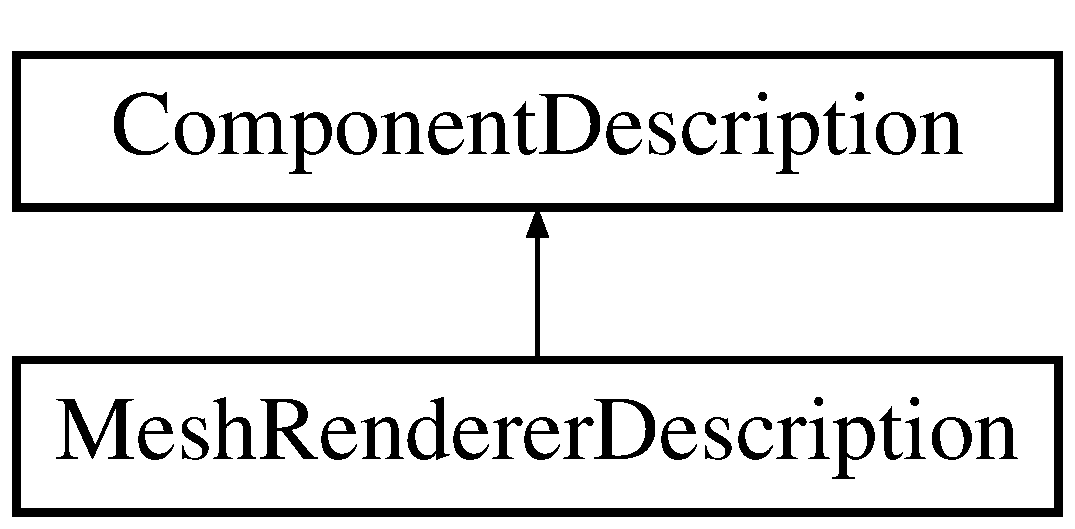
\includegraphics[height=2.000000cm]{class_mesh_renderer_description}
\end{center}
\end{figure}
\subsection*{Public Member Functions}
\begin{DoxyCompactItemize}
\item 
\hypertarget{class_mesh_renderer_description_aa40317aa38cb73fb2d8ff1593043461d}{}{\bfseries Mesh\+Renderer\+Description} (int id)\label{class_mesh_renderer_description_aa40317aa38cb73fb2d8ff1593043461d}

\end{DoxyCompactItemize}
\subsection*{Public Attributes}
\begin{DoxyCompactItemize}
\item 
\hypertarget{class_mesh_renderer_description_ae22fbdf80f02ef9255b74af99d81cfd8}{}int {\bfseries material\+I\+D}\label{class_mesh_renderer_description_ae22fbdf80f02ef9255b74af99d81cfd8}

\end{DoxyCompactItemize}


The documentation for this class was generated from the following file\+:\begin{DoxyCompactItemize}
\item 
/\+Users/guilherme\+\_\+cunha/\+Dev/\+G\+I\+T\+H\+U\+B/\+G\+U\+Inity/\+Source/Serialization\+Structs.\+hpp\end{DoxyCompactItemize}

\hypertarget{struct_mesh_vertex}{}\section{Mesh\+Vertex Struct Reference}
\label{struct_mesh_vertex}\index{Mesh\+Vertex@{Mesh\+Vertex}}
\subsection*{Public Member Functions}
\begin{DoxyCompactItemize}
\item 
\hypertarget{struct_mesh_vertex_a15d2eb5d5fb10a50f590c66c5ae218fd}{}{\bfseries Mesh\+Vertex} (glm\+::vec3 p, glm\+::vec2 u, glm\+::vec3 n)\label{struct_mesh_vertex_a15d2eb5d5fb10a50f590c66c5ae218fd}

\end{DoxyCompactItemize}
\subsection*{Public Attributes}
\begin{DoxyCompactItemize}
\item 
\hypertarget{struct_mesh_vertex_af424f4ac16e7aa6359862ee38fbaf309}{}glm\+::vec3 {\bfseries position}\label{struct_mesh_vertex_af424f4ac16e7aa6359862ee38fbaf309}

\item 
\hypertarget{struct_mesh_vertex_a33831d8380f887676941c4fa8d11f756}{}glm\+::vec2 {\bfseries uv}\label{struct_mesh_vertex_a33831d8380f887676941c4fa8d11f756}

\item 
\hypertarget{struct_mesh_vertex_a9bd172f6367dd18d5a3537a0c1d4c72a}{}glm\+::vec3 {\bfseries normal}\label{struct_mesh_vertex_a9bd172f6367dd18d5a3537a0c1d4c72a}

\end{DoxyCompactItemize}


The documentation for this struct was generated from the following file\+:\begin{DoxyCompactItemize}
\item 
/\+Users/guilherme\+\_\+cunha/\+Dev/\+G\+I\+T\+H\+U\+B/\+G\+U\+Inity/\+Source/Mesh.\+hpp\end{DoxyCompactItemize}

\hypertarget{class_move_handle}{}\section{Move\+Handle Class Reference}
\label{class_move_handle}\index{Move\+Handle@{Move\+Handle}}
Inheritance diagram for Move\+Handle\+:\begin{figure}[H]
\begin{center}
\leavevmode
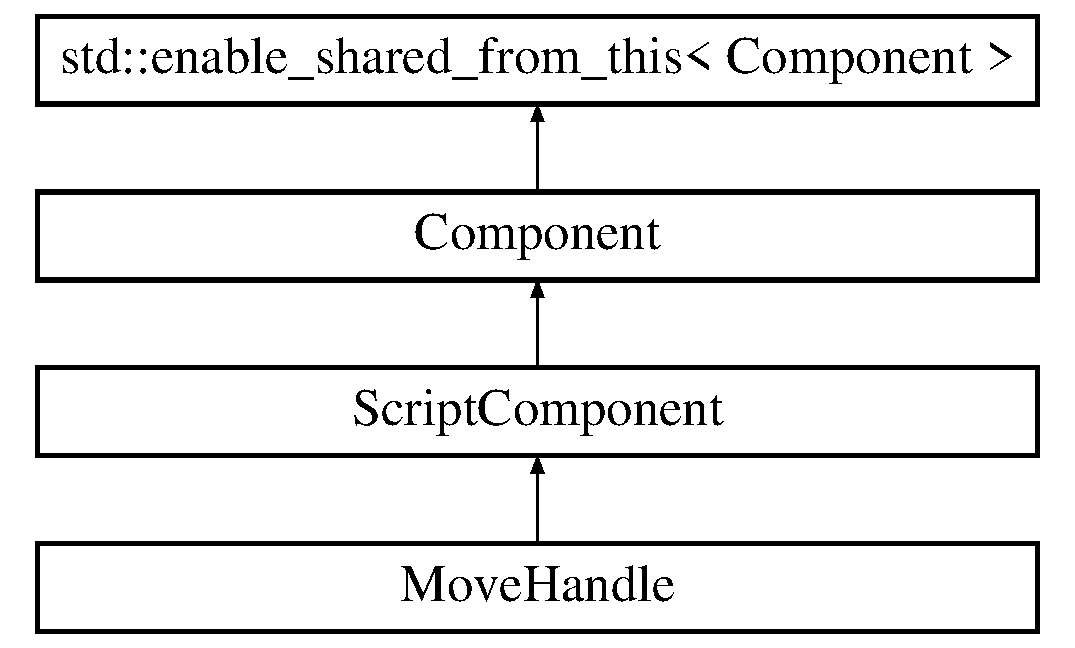
\includegraphics[height=4.000000cm]{class_move_handle}
\end{center}
\end{figure}
\subsection*{Public Member Functions}
\begin{DoxyCompactItemize}
\item 
\hypertarget{class_move_handle_a20df8bf30dd3b8e0fd0173b6de610a9f}{}void {\bfseries set\+Axis} (Move\+Axis axis)\label{class_move_handle_a20df8bf30dd3b8e0fd0173b6de610a9f}

\item 
virtual void \hyperlink{class_move_handle_a39cb33cbbf841fee4d07c8a8cc380128}{tick} (float delta\+Seconds) override
\end{DoxyCompactItemize}
\subsection*{Public Attributes}
\begin{DoxyCompactItemize}
\item 
\hypertarget{class_move_handle_a229b7cb6c45728c807f98794f5f32936}{}Move\+Axis {\bfseries axis}\label{class_move_handle_a229b7cb6c45728c807f98794f5f32936}

\end{DoxyCompactItemize}
\subsection*{Additional Inherited Members}


\subsection{Member Function Documentation}
\hypertarget{class_move_handle_a39cb33cbbf841fee4d07c8a8cc380128}{}\index{Move\+Handle@{Move\+Handle}!tick@{tick}}
\index{tick@{tick}!Move\+Handle@{Move\+Handle}}
\subsubsection[{tick(float delta\+Seconds) override}]{\setlength{\rightskip}{0pt plus 5cm}void Move\+Handle\+::tick (
\begin{DoxyParamCaption}
\item[{float}]{delta\+Secods}
\end{DoxyParamCaption}
)\hspace{0.3cm}{\ttfamily [override]}, {\ttfamily [virtual]}}\label{class_move_handle_a39cb33cbbf841fee4d07c8a8cc380128}
\hyperlink{class_component}{Component} tick override 
\begin{DoxyParams}[1]{Parameters}
\mbox{\tt in}  & {\em delta\+Seconds} & last frame durations \\
\hline
\end{DoxyParams}


Reimplemented from \hyperlink{class_script_component_aa765fa62a343a8d83eb168d369b93a51}{Script\+Component}.



The documentation for this class was generated from the following files\+:\begin{DoxyCompactItemize}
\item 
/\+Users/guilherme\+\_\+cunha/\+Dev/\+G\+I\+T\+H\+U\+B/\+G\+U\+Inity/\+Source/Move\+Handle.\+hpp\item 
/\+Users/guilherme\+\_\+cunha/\+Dev/\+G\+I\+T\+H\+U\+B/\+G\+U\+Inity/\+Source/Move\+Handle.\+cpp\end{DoxyCompactItemize}

\hypertarget{class_move_tool}{}\section{Move\+Tool Class Reference}
\label{class_move_tool}\index{Move\+Tool@{Move\+Tool}}
Inheritance diagram for Move\+Tool\+:\begin{figure}[H]
\begin{center}
\leavevmode
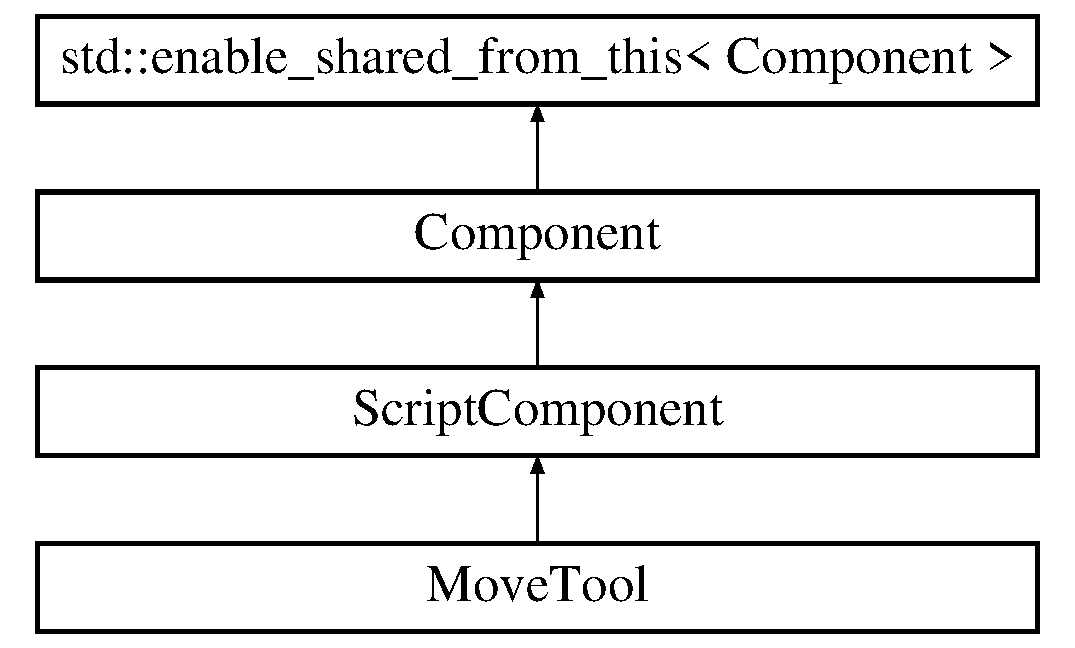
\includegraphics[height=4.000000cm]{class_move_tool}
\end{center}
\end{figure}
\subsection*{Public Member Functions}
\begin{DoxyCompactItemize}
\item 
virtual void \hyperlink{class_move_tool_ac53066bdb36f2e01234fa58a20cc1f0d}{awake} () override
\item 
virtual void \hyperlink{class_move_tool_ad38e6fcb03e6d7b2f0ef241ec0eb5271}{tick} (float delta\+Seconds) override
\end{DoxyCompactItemize}
\subsection*{Public Attributes}
\begin{DoxyCompactItemize}
\item 
\hypertarget{class_move_tool_ada6e1ed12bb8d8e570611f962c69bd39}{}Move\+Mode {\bfseries move\+Mode}\label{class_move_tool_ada6e1ed12bb8d8e570611f962c69bd39}

\item 
\hypertarget{class_move_tool_a8f32b2f996a05392a0792d2ea4eb6320}{}weak\+\_\+ptr$<$ \hyperlink{class_move_handle}{Move\+Handle} $>$ {\bfseries forward}\label{class_move_tool_a8f32b2f996a05392a0792d2ea4eb6320}

\item 
\hypertarget{class_move_tool_aa2af9be79e0ac6067ff7e703b748a207}{}weak\+\_\+ptr$<$ \hyperlink{class_move_handle}{Move\+Handle} $>$ {\bfseries up}\label{class_move_tool_aa2af9be79e0ac6067ff7e703b748a207}

\item 
\hypertarget{class_move_tool_ab969dce017261f3da61e15db134872ad}{}weak\+\_\+ptr$<$ \hyperlink{class_move_handle}{Move\+Handle} $>$ {\bfseries right}\label{class_move_tool_ab969dce017261f3da61e15db134872ad}

\end{DoxyCompactItemize}
\subsection*{Additional Inherited Members}


\subsection{Member Function Documentation}
\hypertarget{class_move_tool_ac53066bdb36f2e01234fa58a20cc1f0d}{}\index{Move\+Tool@{Move\+Tool}!awake@{awake}}
\index{awake@{awake}!Move\+Tool@{Move\+Tool}}
\subsubsection[{awake() override}]{\setlength{\rightskip}{0pt plus 5cm}void Move\+Tool\+::awake (
\begin{DoxyParamCaption}
{}
\end{DoxyParamCaption}
)\hspace{0.3cm}{\ttfamily [override]}, {\ttfamily [virtual]}}\label{class_move_tool_ac53066bdb36f2e01234fa58a20cc1f0d}
\hyperlink{class_component}{Component} awake override 

Reimplemented from \hyperlink{class_script_component_a4667b8a3712e18b25cd6f49f12c5677d}{Script\+Component}.

\hypertarget{class_move_tool_ad38e6fcb03e6d7b2f0ef241ec0eb5271}{}\index{Move\+Tool@{Move\+Tool}!tick@{tick}}
\index{tick@{tick}!Move\+Tool@{Move\+Tool}}
\subsubsection[{tick(float delta\+Seconds) override}]{\setlength{\rightskip}{0pt plus 5cm}void Move\+Tool\+::tick (
\begin{DoxyParamCaption}
\item[{float}]{delta\+Secods}
\end{DoxyParamCaption}
)\hspace{0.3cm}{\ttfamily [override]}, {\ttfamily [virtual]}}\label{class_move_tool_ad38e6fcb03e6d7b2f0ef241ec0eb5271}
\hyperlink{class_component}{Component} tick override 
\begin{DoxyParams}[1]{Parameters}
\mbox{\tt in}  & {\em delta\+Seconds} & last frame durations \\
\hline
\end{DoxyParams}


Reimplemented from \hyperlink{class_script_component_aa765fa62a343a8d83eb168d369b93a51}{Script\+Component}.



The documentation for this class was generated from the following files\+:\begin{DoxyCompactItemize}
\item 
/\+Users/guilherme\+\_\+cunha/\+Dev/\+G\+I\+T\+H\+U\+B/\+G\+U\+Inity/\+Source/Move\+Tool.\+hpp\item 
/\+Users/guilherme\+\_\+cunha/\+Dev/\+G\+I\+T\+H\+U\+B/\+G\+U\+Inity/\+Source/Move\+Tool.\+cpp\end{DoxyCompactItemize}

\hypertarget{class_observer}{}\section{Observer Class Reference}
\label{class_observer}\index{Observer@{Observer}}
Inheritance diagram for Observer\+:\begin{figure}[H]
\begin{center}
\leavevmode
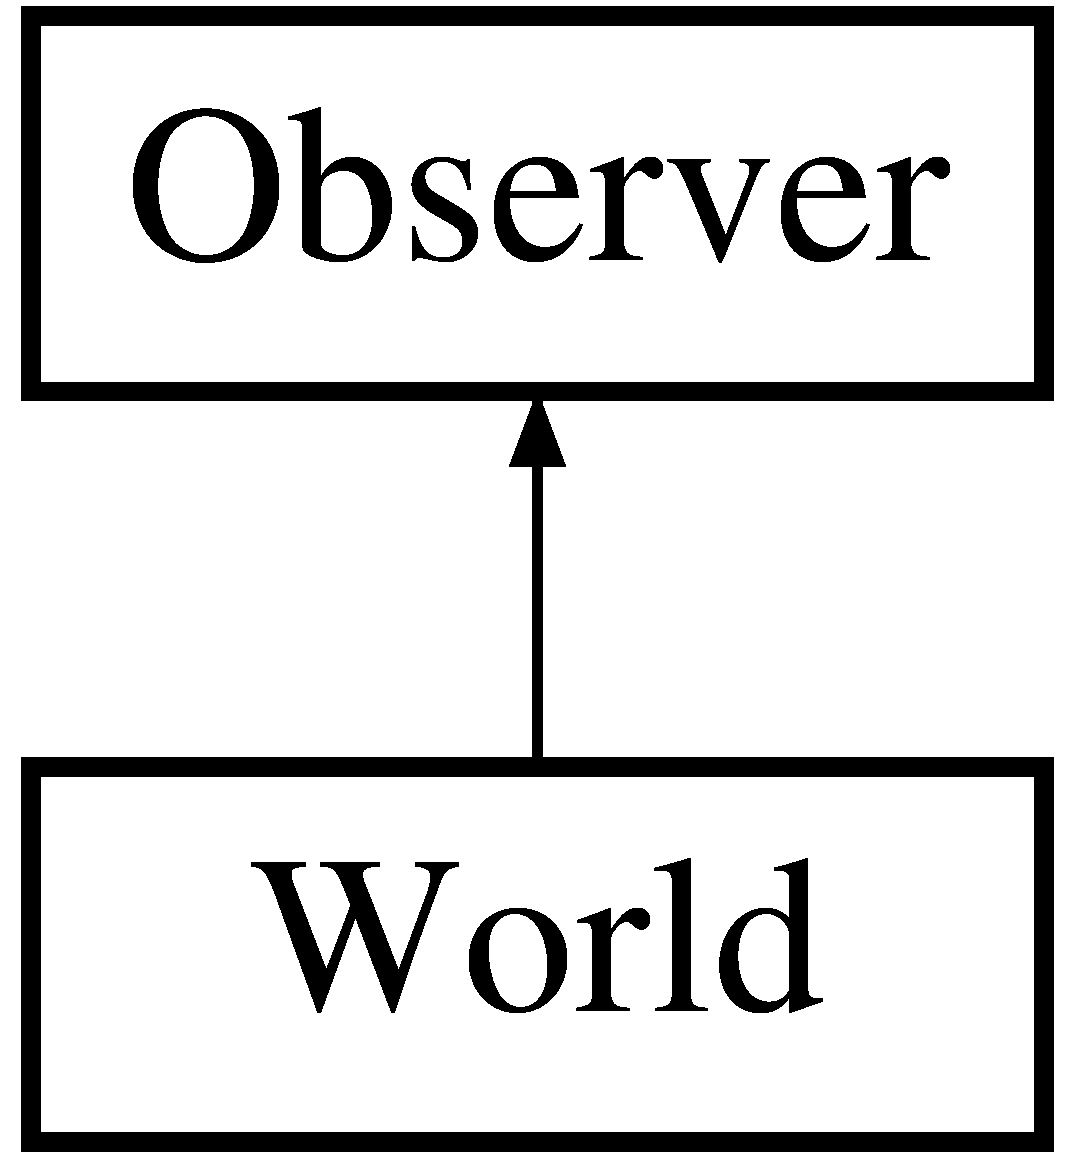
\includegraphics[height=2.000000cm]{class_observer}
\end{center}
\end{figure}
\subsection*{Public Member Functions}
\begin{DoxyCompactItemize}
\item 
\hypertarget{class_observer_ab9deb73c274eec9442cf94b63b1bee57}{}virtual void {\bfseries on\+Notify} (Component\+Event\+Type type, shared\+\_\+ptr$<$ \hyperlink{class_component}{Component} $>$ component, bool is\+Editor)=0\label{class_observer_ab9deb73c274eec9442cf94b63b1bee57}

\item 
\hypertarget{class_observer_a982c319d757f7b82cfd47f3da2db9c76}{}virtual void {\bfseries on\+Notify} (Actor\+Event\+Type type, shared\+\_\+ptr$<$ \hyperlink{class_actor}{Actor} $>$ actor, bool is\+Editor)=0\label{class_observer_a982c319d757f7b82cfd47f3da2db9c76}

\end{DoxyCompactItemize}


The documentation for this class was generated from the following files\+:\begin{DoxyCompactItemize}
\item 
/\+Users/guilherme\+\_\+cunha/\+Dev/\+G\+I\+T\+H\+U\+B/\+G\+U\+Inity/\+Source/Observer.\+hpp\item 
/\+Users/guilherme\+\_\+cunha/\+Dev/\+G\+I\+T\+H\+U\+B/\+G\+U\+Inity/\+Source/Observer.\+cpp\end{DoxyCompactItemize}

\hypertarget{struct_packed_f_b_x_vertex}{}\section{Packed\+F\+B\+X\+Vertex Struct Reference}
\label{struct_packed_f_b_x_vertex}\index{Packed\+F\+B\+X\+Vertex@{Packed\+F\+B\+X\+Vertex}}
\subsection*{Public Member Functions}
\begin{DoxyCompactItemize}
\item 
\hypertarget{struct_packed_f_b_x_vertex_a1ba1197fe8f7af21b7101103efc8df3c}{}bool {\bfseries operator$<$} (const \hyperlink{struct_packed_f_b_x_vertex}{Packed\+F\+B\+X\+Vertex} that) const \label{struct_packed_f_b_x_vertex_a1ba1197fe8f7af21b7101103efc8df3c}

\end{DoxyCompactItemize}
\subsection*{Public Attributes}
\begin{DoxyCompactItemize}
\item 
\hypertarget{struct_packed_f_b_x_vertex_abe1bcb951c649572cf51651919478d2d}{}Fbx\+Vector4 {\bfseries position}\label{struct_packed_f_b_x_vertex_abe1bcb951c649572cf51651919478d2d}

\item 
\hypertarget{struct_packed_f_b_x_vertex_a2dd7a654090fb00ef766d4800b82032c}{}Fbx\+Vector2 {\bfseries uv}\label{struct_packed_f_b_x_vertex_a2dd7a654090fb00ef766d4800b82032c}

\item 
\hypertarget{struct_packed_f_b_x_vertex_a524a5cd20f3df4b5c8e9b11880444819}{}Fbx\+Vector4 {\bfseries normal}\label{struct_packed_f_b_x_vertex_a524a5cd20f3df4b5c8e9b11880444819}

\end{DoxyCompactItemize}


The documentation for this struct was generated from the following file\+:\begin{DoxyCompactItemize}
\item 
/\+Users/guilherme\+\_\+cunha/\+Dev/\+G\+I\+T\+H\+U\+B/\+G\+U\+Inity/\+Source/Mesh\+Importer.\+hpp\end{DoxyCompactItemize}

\hypertarget{struct_packed_o_b_j_vertex}{}\section{Packed\+O\+B\+J\+Vertex Struct Reference}
\label{struct_packed_o_b_j_vertex}\index{Packed\+O\+B\+J\+Vertex@{Packed\+O\+B\+J\+Vertex}}
\subsection*{Public Member Functions}
\begin{DoxyCompactItemize}
\item 
\hypertarget{struct_packed_o_b_j_vertex_a66d540de278b1bd89d0e386ac9141124}{}bool {\bfseries operator$<$} (const \hyperlink{struct_packed_o_b_j_vertex}{Packed\+O\+B\+J\+Vertex} that) const \label{struct_packed_o_b_j_vertex_a66d540de278b1bd89d0e386ac9141124}

\end{DoxyCompactItemize}
\subsection*{Public Attributes}
\begin{DoxyCompactItemize}
\item 
\hypertarget{struct_packed_o_b_j_vertex_a6a6dcdb4fa928144595b922fc4f05269}{}glm\+::vec3 {\bfseries position}\label{struct_packed_o_b_j_vertex_a6a6dcdb4fa928144595b922fc4f05269}

\item 
\hypertarget{struct_packed_o_b_j_vertex_a2aa0bcdf0686313becf6de277ab7c47a}{}glm\+::vec2 {\bfseries uv}\label{struct_packed_o_b_j_vertex_a2aa0bcdf0686313becf6de277ab7c47a}

\item 
\hypertarget{struct_packed_o_b_j_vertex_a3c6529f9a8518a5a807241438f70a24f}{}glm\+::vec3 {\bfseries normal}\label{struct_packed_o_b_j_vertex_a3c6529f9a8518a5a807241438f70a24f}

\end{DoxyCompactItemize}


The documentation for this struct was generated from the following file\+:\begin{DoxyCompactItemize}
\item 
/\+Users/guilherme\+\_\+cunha/\+Dev/\+G\+I\+T\+H\+U\+B/\+G\+U\+Inity/\+Source/Mesh\+Importer.\+hpp\end{DoxyCompactItemize}

\hypertarget{class_person}{}\section{Person Class Reference}
\label{class_person}\index{Person@{Person}}
\subsection*{Public Attributes}
\begin{DoxyCompactItemize}
\item 
\hypertarget{class_person_a669b64897b4d823a27bb5866368d4dfa}{}string {\bfseries name}\label{class_person_a669b64897b4d823a27bb5866368d4dfa}

\item 
\hypertarget{class_person_acf9db1a60683f40b20ae569d29852d69}{}int {\bfseries age}\label{class_person_acf9db1a60683f40b20ae569d29852d69}

\end{DoxyCompactItemize}


The documentation for this class was generated from the following file\+:\begin{DoxyCompactItemize}
\item 
/\+Users/guilherme\+\_\+cunha/\+Dev/\+G\+I\+T\+H\+U\+B/\+G\+U\+Inity/\+Source/Reflection\+Test.\+h\end{DoxyCompactItemize}

\hypertarget{class_physics}{}\section{Physics Class Reference}
\label{class_physics}\index{Physics@{Physics}}
\subsection*{Public Member Functions}
\begin{DoxyCompactItemize}
\item 
\hypertarget{class_physics_ae1a4865b4344594f83a6e5e0baad2a9a}{}int {\bfseries init} ()\label{class_physics_ae1a4865b4344594f83a6e5e0baad2a9a}

\end{DoxyCompactItemize}
\subsection*{Static Public Member Functions}
\begin{DoxyCompactItemize}
\item 
\hypertarget{class_physics_a6989c20a392877d24738ec1b05e9e22b}{}static bool {\bfseries ray\+Cast} (Px\+Scene $\ast$scene, const \hyperlink{class_ray}{Ray} \&r, const float distance, Px\+Raycast\+Buffer \&hit\+Callback)\label{class_physics_a6989c20a392877d24738ec1b05e9e22b}

\item 
\hypertarget{class_physics_a13d6c1dfe0b3441343bb0d30a498c5ce}{}static void {\bfseries update\+Actors\+Transform} (Px\+Scene $\ast$scene)\label{class_physics_a13d6c1dfe0b3441343bb0d30a498c5ce}

\item 
\hypertarget{class_physics_ae59d1a2bd0dc9bc2ad54074a1a6b43ec}{}static Px\+Rigid\+Dynamic $\ast$ {\bfseries create\+Rigid\+Dynamic} (shared\+\_\+ptr$<$ \hyperlink{class_actor}{Actor} $>$ actor)\label{class_physics_ae59d1a2bd0dc9bc2ad54074a1a6b43ec}

\item 
\hypertarget{class_physics_aa7faba18fc0143b4ddaae52eca219716}{}static Px\+D6\+Joint $\ast$ {\bfseries create\+D6\+Joint} (shared\+\_\+ptr$<$ \hyperlink{class_actor}{Actor} $>$ actor, Px\+Rigid\+Body $\ast$rigid\+Body)\label{class_physics_aa7faba18fc0143b4ddaae52eca219716}

\item 
\hypertarget{class_physics_a763587f080bb42879a8fa10d009e44fe}{}static Px\+Shape $\ast$ {\bfseries create\+Box\+Collider} (glm\+::vec3 half\+Extent, glm\+::vec3 center, shared\+\_\+ptr$<$ \hyperlink{class_actor}{Actor} $>$ actor)\label{class_physics_a763587f080bb42879a8fa10d009e44fe}

\item 
\hypertarget{class_physics_ae6015ef65348a1c01a85d2e079d35eac}{}static Px\+Shape $\ast$ {\bfseries create\+Box\+Collider} (Px\+Vec3 half\+Extent, Px\+Vec3 center, shared\+\_\+ptr$<$ \hyperlink{class_actor}{Actor} $>$ actor)\label{class_physics_ae6015ef65348a1c01a85d2e079d35eac}

\item 
\hypertarget{class_physics_a2ef2359f0d22c30244dcbb98e707e52b}{}static Px\+Shape $\ast$ {\bfseries create\+Box\+Collider} (shared\+\_\+ptr$<$ \hyperlink{class_actor}{Actor} $>$ actor)\label{class_physics_a2ef2359f0d22c30244dcbb98e707e52b}

\item 
\hypertarget{class_physics_a5a259da34b27da97a4fc5ae046b844db}{}static Px\+Shape $\ast$ {\bfseries create\+Sphere\+Collider} (float radius, glm\+::vec3 center, shared\+\_\+ptr$<$ \hyperlink{class_actor}{Actor} $>$ actor)\label{class_physics_a5a259da34b27da97a4fc5ae046b844db}

\item 
\hypertarget{class_physics_a54b03c18d6a9cef0934ed0e5ba4d1664}{}static Px\+Shape $\ast$ {\bfseries create\+Sphere\+Collider} (float radius, Px\+Vec3 center, shared\+\_\+ptr$<$ \hyperlink{class_actor}{Actor} $>$ actor)\label{class_physics_a54b03c18d6a9cef0934ed0e5ba4d1664}

\item 
\hypertarget{class_physics_a62ed5a7e6561543d40284b1316c9e6f1}{}static Px\+Shape $\ast$ {\bfseries create\+Sphere\+Collider} (shared\+\_\+ptr$<$ \hyperlink{class_actor}{Actor} $>$ actor)\label{class_physics_a62ed5a7e6561543d40284b1316c9e6f1}

\item 
\hypertarget{class_physics_ae1f6e27ae24c88616eac4199329c2474}{}static void {\bfseries set\+Capsule\+Orientation} (Px\+Shape $\ast$shape, Rotate\+Axis orientation)\label{class_physics_ae1f6e27ae24c88616eac4199329c2474}

\item 
\hypertarget{class_physics_af667feaa16f54d7ba980b0535efdd725}{}static Px\+Shape $\ast$ {\bfseries create\+Capsule\+Collider} (float radius, float half\+Height, Rotate\+Axis orientation, glm\+::vec3 center, shared\+\_\+ptr$<$ \hyperlink{class_actor}{Actor} $>$ actor)\label{class_physics_af667feaa16f54d7ba980b0535efdd725}

\item 
\hypertarget{class_physics_ad61bf2c7fdb5b7f6263cb45801d80fa2}{}static Px\+Shape $\ast$ {\bfseries create\+Capsule\+Collider} (float radius, float half\+Height, Rotate\+Axis orientation, Px\+Vec3 center, shared\+\_\+ptr$<$ \hyperlink{class_actor}{Actor} $>$ actor)\label{class_physics_ad61bf2c7fdb5b7f6263cb45801d80fa2}

\item 
\hypertarget{class_physics_ab0918271779efbfbba18a39f7ee9e88a}{}static Px\+Shape $\ast$ {\bfseries create\+Capsule\+Collider} (shared\+\_\+ptr$<$ \hyperlink{class_actor}{Actor} $>$ actor)\label{class_physics_ab0918271779efbfbba18a39f7ee9e88a}

\item 
\hypertarget{class_physics_a2408727ec00753afccccdd949ed45d4e}{}static Px\+Shape $\ast$ {\bfseries create\+Mesh\+Collider} (shared\+\_\+ptr$<$ \hyperlink{class_actor}{Actor} $>$ actor)\label{class_physics_a2408727ec00753afccccdd949ed45d4e}

\item 
\hypertarget{class_physics_a88e2aee7aea3b14821dd1f29061d30d2}{}static Px\+Convex\+Mesh $\ast$ {\bfseries get\+Px\+Convex\+Mesh} (shared\+\_\+ptr$<$ \hyperlink{class_mesh}{Mesh} $>$ mesh)\label{class_physics_a88e2aee7aea3b14821dd1f29061d30d2}

\item 
\hypertarget{class_physics_a0860be4d01d8f3ac3091bce1f4fd6654}{}static Px\+Scene $\ast$ {\bfseries create\+Physics\+Scene} ()\label{class_physics_a0860be4d01d8f3ac3091bce1f4fd6654}

\item 
\hypertarget{class_physics_a5c3d81bc67f81136181db76358b0ede7}{}static Px\+Material $\ast$ {\bfseries create\+Material} (float friction, float dynamic\+Friction, float restitution)\label{class_physics_a5c3d81bc67f81136181db76358b0ede7}

\item 
\hypertarget{class_physics_af324ec30b84e67fbe463f0a14d491b50}{}static shared\+\_\+ptr$<$ \hyperlink{class_physics_material}{Physics\+Material} $>$ {\bfseries get\+Default\+Material} ()\label{class_physics_af324ec30b84e67fbe463f0a14d491b50}

\item 
\hypertarget{class_physics_ac8d328e039f44a45b08742d35e434c94}{}static void {\bfseries tick\+Scene} (Px\+Scene $\ast$scene)\label{class_physics_ac8d328e039f44a45b08742d35e434c94}

\item 
\hypertarget{class_physics_a9594de74882adb25ce75ebc8b34fd6ce}{}static void {\bfseries shutdown} ()\label{class_physics_a9594de74882adb25ce75ebc8b34fd6ce}

\item 
\hypertarget{class_physics_a351ceac4e3a916796cc3b89c49133664}{}static bool {\bfseries convex\+Mesh\+Computed} (shared\+\_\+ptr$<$ \hyperlink{class_mesh}{Mesh} $>$ mesh)\label{class_physics_a351ceac4e3a916796cc3b89c49133664}

\end{DoxyCompactItemize}
\subsection*{Static Public Attributes}
\begin{DoxyCompactItemize}
\item 
\hypertarget{class_physics_a2ad3728dd5522f3f424bda60399ccf88}{}static Px\+Physics $\ast$ {\bfseries g\+Physics\+S\+D\+K}\label{class_physics_a2ad3728dd5522f3f424bda60399ccf88}

\item 
\hypertarget{class_physics_a0e40ffb4cbbffabfbb85f074a0425f8c}{}static Px\+Default\+Error\+Callback {\bfseries g\+Default\+Error\+Callback}\label{class_physics_a0e40ffb4cbbffabfbb85f074a0425f8c}

\item 
\hypertarget{class_physics_a19b2ae365f967634785f9d70a532c02f}{}static Px\+Default\+Allocator {\bfseries g\+Default\+Allocator\+Callback}\label{class_physics_a19b2ae365f967634785f9d70a532c02f}

\item 
\hypertarget{class_physics_acfcee285f1920dd0d3efa4a9d6188b9f}{}static Px\+Foundation $\ast$ {\bfseries g\+Foundation}\label{class_physics_acfcee285f1920dd0d3efa4a9d6188b9f}

\item 
\hypertarget{class_physics_a19cc5586e2a87e6984b6c5d044040b83}{}static \hyperlink{class_phys_x_event_callback}{Phys\+X\+Event\+Callback} $\ast$ {\bfseries physx\+Event\+Callback}\label{class_physics_a19cc5586e2a87e6984b6c5d044040b83}

\item 
\hypertarget{class_physics_a2cefc51f88c56b800fc3d1de56223132}{}static Px\+Real {\bfseries my\+Timestep} = 1.\+0f / 60.\+0f\label{class_physics_a2cefc51f88c56b800fc3d1de56223132}

\item 
\hypertarget{class_physics_afaa14c98236618242d15a8e2a15ee88c}{}static map$<$ shared\+\_\+ptr$<$ \hyperlink{class_mesh}{Mesh} $>$, Px\+Convex\+Mesh $\ast$ $>$ {\bfseries convex\+Meshes}\label{class_physics_afaa14c98236618242d15a8e2a15ee88c}

\end{DoxyCompactItemize}


The documentation for this class was generated from the following files\+:\begin{DoxyCompactItemize}
\item 
/\+Users/guilherme\+\_\+cunha/\+Dev/\+G\+I\+T\+H\+U\+B/\+G\+U\+Inity/\+Source/Physics.\+hpp\item 
/\+Users/guilherme\+\_\+cunha/\+Dev/\+G\+I\+T\+H\+U\+B/\+G\+U\+Inity/\+Source/Physics.\+cpp\end{DoxyCompactItemize}

\hypertarget{class_physics_material}{}\section{Physics\+Material Class Reference}
\label{class_physics_material}\index{Physics\+Material@{Physics\+Material}}
Inheritance diagram for Physics\+Material\+:\begin{figure}[H]
\begin{center}
\leavevmode
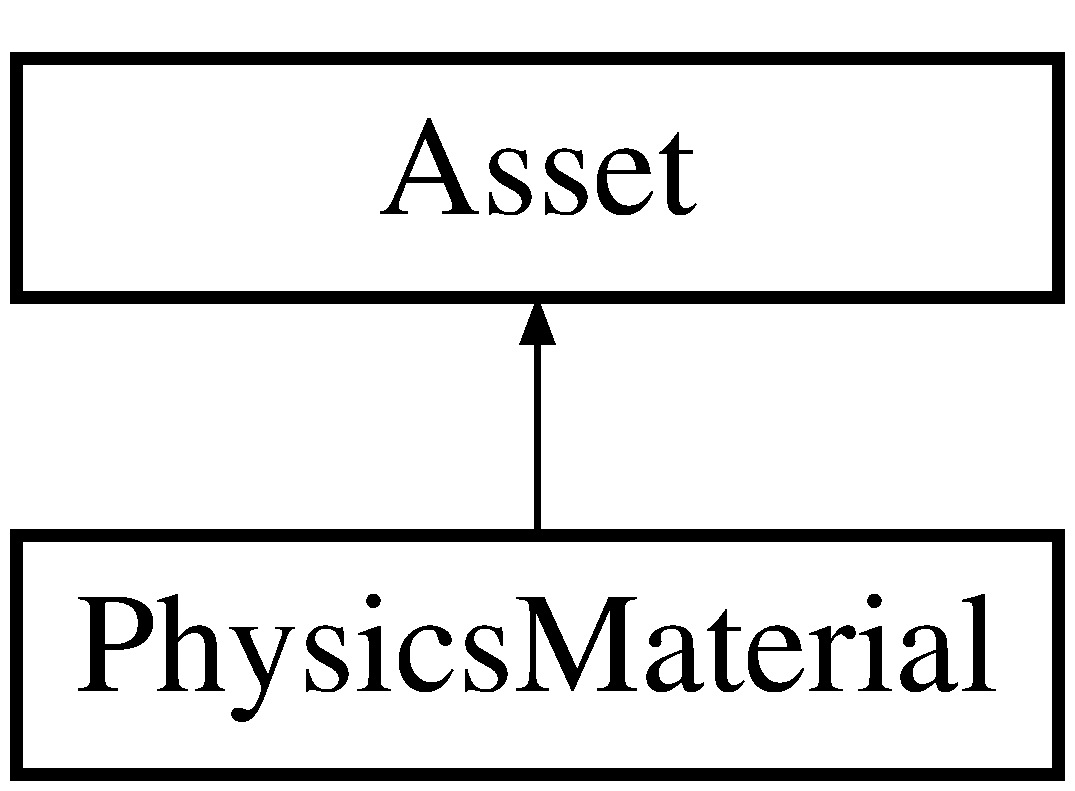
\includegraphics[height=2.000000cm]{class_physics_material}
\end{center}
\end{figure}
\subsection*{Public Member Functions}
\begin{DoxyCompactItemize}
\item 
\hypertarget{class_physics_material_ad7ba381e5ff323b9377ab562fada3425}{}{\bfseries Physics\+Material} (float friction, float dynamic\+Friction, float restitution)\label{class_physics_material_ad7ba381e5ff323b9377ab562fada3425}

\item 
\hypertarget{class_physics_material_a36ecb77c53c3ef3e52c6f867be156f96}{}Px\+Material $\ast$ {\bfseries get\+Material} ()\label{class_physics_material_a36ecb77c53c3ef3e52c6f867be156f96}

\end{DoxyCompactItemize}
\subsection*{Public Attributes}
\begin{DoxyCompactItemize}
\item 
\hypertarget{class_physics_material_a40499e7e0af0b5a17c412b23bb6d98a4}{}float {\bfseries friction}\label{class_physics_material_a40499e7e0af0b5a17c412b23bb6d98a4}

\item 
\hypertarget{class_physics_material_a6ede2c7f6bdaef3a2ee60667a6e6a546}{}float {\bfseries dynamic\+Friction}\label{class_physics_material_a6ede2c7f6bdaef3a2ee60667a6e6a546}

\item 
\hypertarget{class_physics_material_acf45501fe93570bfb0ea3365941e19c5}{}float {\bfseries restitution}\label{class_physics_material_acf45501fe93570bfb0ea3365941e19c5}

\end{DoxyCompactItemize}


The documentation for this class was generated from the following files\+:\begin{DoxyCompactItemize}
\item 
/\+Users/guilherme\+\_\+cunha/\+Dev/\+G\+I\+T\+H\+U\+B/\+G\+U\+Inity/\+Source/Physics\+Material.\+hpp\item 
/\+Users/guilherme\+\_\+cunha/\+Dev/\+G\+I\+T\+H\+U\+B/\+G\+U\+Inity/\+Source/Physics\+Material.\+cpp\end{DoxyCompactItemize}

\hypertarget{class_phys_x_allocator_callback}{}\section{Phys\+X\+Allocator\+Callback Class Reference}
\label{class_phys_x_allocator_callback}\index{Phys\+X\+Allocator\+Callback@{Phys\+X\+Allocator\+Callback}}
Inheritance diagram for Phys\+X\+Allocator\+Callback\+:\begin{figure}[H]
\begin{center}
\leavevmode
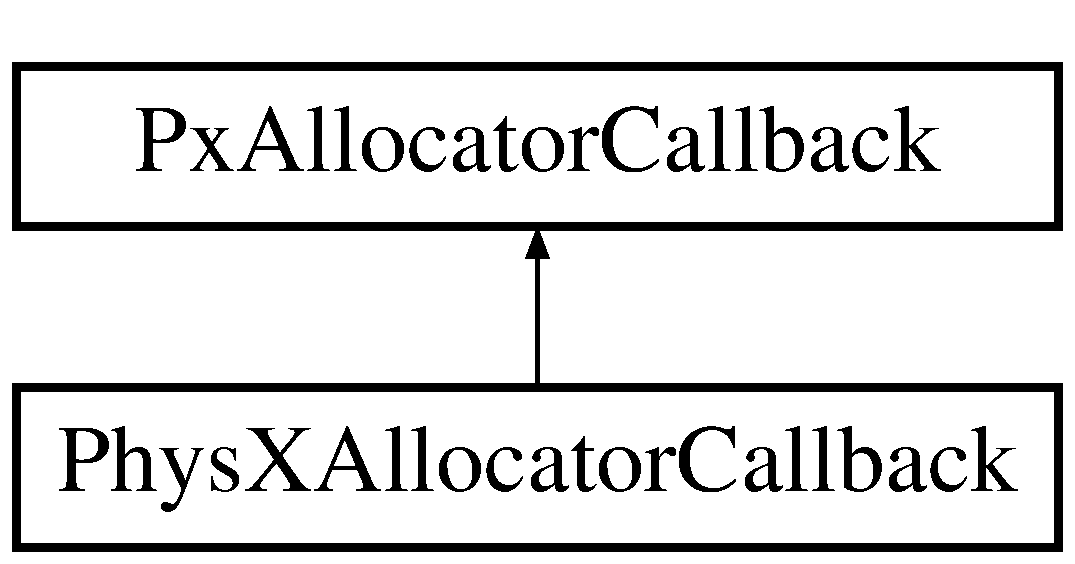
\includegraphics[height=2.000000cm]{class_phys_x_allocator_callback}
\end{center}
\end{figure}
\subsection*{Public Member Functions}
\begin{DoxyCompactItemize}
\item 
\hypertarget{class_phys_x_allocator_callback_a5757eeeebbb1467b08436a6c38fdd642}{}void $\ast$ {\bfseries allocate} (size\+\_\+t size, const char $\ast$, const char $\ast$, int)\label{class_phys_x_allocator_callback_a5757eeeebbb1467b08436a6c38fdd642}

\item 
\hypertarget{class_phys_x_allocator_callback_a1043ba91a80459c8d6bfd4df345d8b1b}{}void {\bfseries deallocate} (void $\ast$ptr)\label{class_phys_x_allocator_callback_a1043ba91a80459c8d6bfd4df345d8b1b}

\end{DoxyCompactItemize}


The documentation for this class was generated from the following files\+:\begin{DoxyCompactItemize}
\item 
/\+Users/guilherme\+\_\+cunha/\+Dev/\+G\+I\+T\+H\+U\+B/\+G\+U\+Inity/\+Source/Phys\+X\+Allocator\+Callback.\+h\item 
/\+Users/guilherme\+\_\+cunha/\+Dev/\+G\+I\+T\+H\+U\+B/\+G\+U\+Inity/\+Source/Phys\+X\+Allocator\+Callback.\+cpp\end{DoxyCompactItemize}

\hypertarget{class_phys_x_event_callback}{}\section{Phys\+X\+Event\+Callback Class Reference}
\label{class_phys_x_event_callback}\index{Phys\+X\+Event\+Callback@{Phys\+X\+Event\+Callback}}
Inheritance diagram for Phys\+X\+Event\+Callback\+:\begin{figure}[H]
\begin{center}
\leavevmode
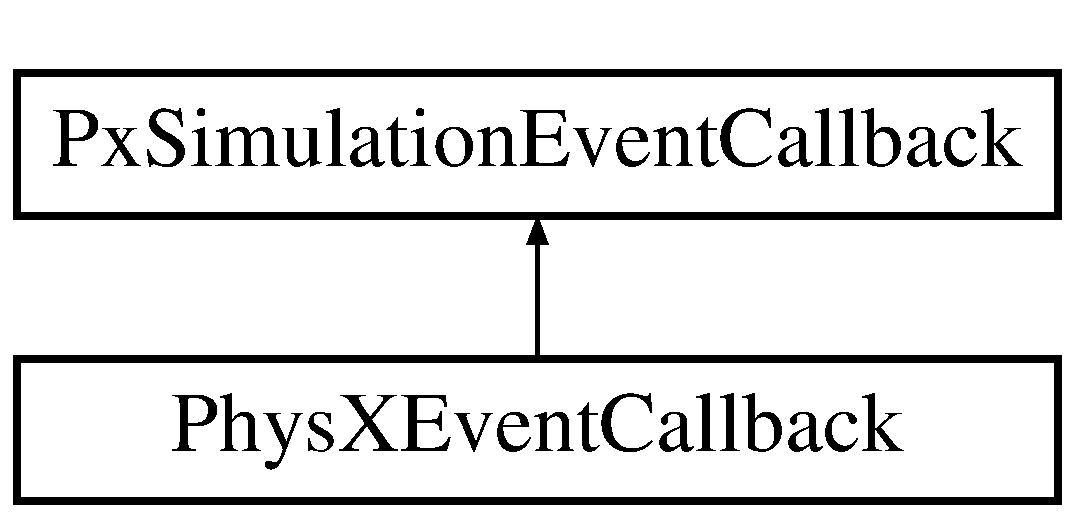
\includegraphics[height=2.000000cm]{class_phys_x_event_callback}
\end{center}
\end{figure}
\subsection*{Public Member Functions}
\begin{DoxyCompactItemize}
\item 
\hypertarget{class_phys_x_event_callback_ae8880546913e485700ce2ee1f7f6f55e}{}virtual void {\bfseries on\+Constraint\+Break} (Px\+Constraint\+Info $\ast$constraints, Px\+U32 count) override\label{class_phys_x_event_callback_ae8880546913e485700ce2ee1f7f6f55e}

\item 
\hypertarget{class_phys_x_event_callback_a630f09dcb2536172a413263765b3c43d}{}virtual void {\bfseries on\+Wake} (Px\+Actor $\ast$$\ast$actors, Px\+U32 count) override\label{class_phys_x_event_callback_a630f09dcb2536172a413263765b3c43d}

\item 
\hypertarget{class_phys_x_event_callback_aafe0aed55517f6a0a0e96b5aba413c4e}{}virtual void {\bfseries on\+Sleep} (Px\+Actor $\ast$$\ast$actors, Px\+U32 count) override\label{class_phys_x_event_callback_aafe0aed55517f6a0a0e96b5aba413c4e}

\item 
\hypertarget{class_phys_x_event_callback_a70b68c082b19901f260799ed5292d1ec}{}virtual void {\bfseries on\+Contact} (const Px\+Contact\+Pair\+Header \&pair\+Header, const Px\+Contact\+Pair $\ast$pairs, Px\+U32 nb\+Pairs) override\label{class_phys_x_event_callback_a70b68c082b19901f260799ed5292d1ec}

\item 
\hypertarget{class_phys_x_event_callback_a513a33261a63b4bb5141766219a5c876}{}virtual void {\bfseries on\+Trigger} (Px\+Trigger\+Pair $\ast$pairs, Px\+U32 count) override\label{class_phys_x_event_callback_a513a33261a63b4bb5141766219a5c876}

\end{DoxyCompactItemize}


The documentation for this class was generated from the following files\+:\begin{DoxyCompactItemize}
\item 
/\+Users/guilherme\+\_\+cunha/\+Dev/\+G\+I\+T\+H\+U\+B/\+G\+U\+Inity/\+Source/Phys\+X\+Event\+Callback.\+hpp\item 
/\+Users/guilherme\+\_\+cunha/\+Dev/\+G\+I\+T\+H\+U\+B/\+G\+U\+Inity/\+Source/Phys\+X\+Event\+Callback.\+cpp\end{DoxyCompactItemize}

\hypertarget{class_phys_x_insertion_callback}{}\section{Phys\+X\+Insertion\+Callback Class Reference}
\label{class_phys_x_insertion_callback}\index{Phys\+X\+Insertion\+Callback@{Phys\+X\+Insertion\+Callback}}
Inheritance diagram for Phys\+X\+Insertion\+Callback\+:\begin{figure}[H]
\begin{center}
\leavevmode
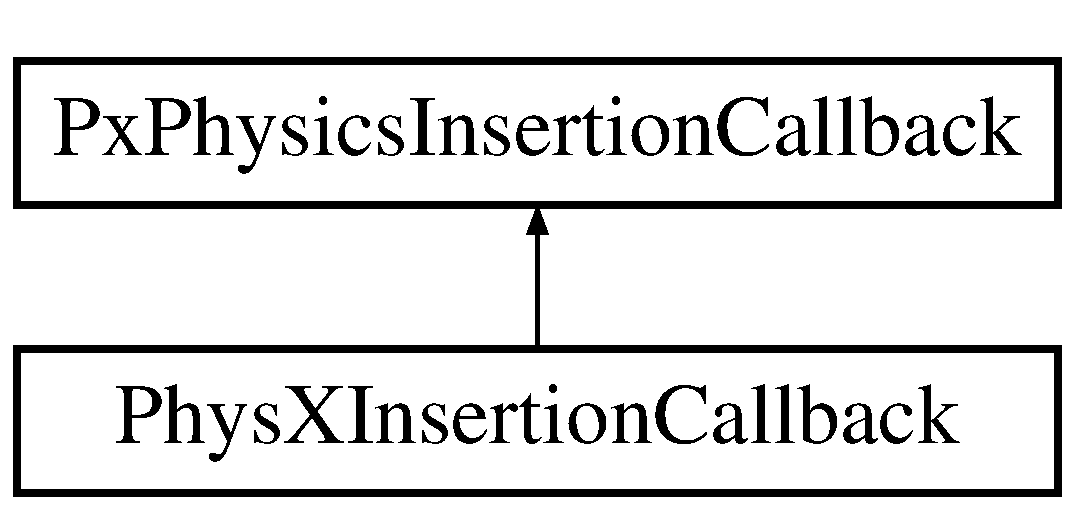
\includegraphics[height=2.000000cm]{class_phys_x_insertion_callback}
\end{center}
\end{figure}


The documentation for this class was generated from the following files\+:\begin{DoxyCompactItemize}
\item 
/\+Users/guilherme\+\_\+cunha/\+Dev/\+G\+I\+T\+H\+U\+B/\+G\+U\+Inity/\+Source/Phys\+X\+Insertion\+Callback.\+h\item 
/\+Users/guilherme\+\_\+cunha/\+Dev/\+G\+I\+T\+H\+U\+B/\+G\+U\+Inity/\+Source/Phys\+X\+Insertion\+Callback.\+cpp\end{DoxyCompactItemize}

\hypertarget{struct_plane}{}\section{Plane Struct Reference}
\label{struct_plane}\index{Plane@{Plane}}


{\ttfamily \#include $<$Math\+Structs.\+hpp$>$}

\subsection*{Public Member Functions}
\begin{DoxyCompactItemize}
\item 
\hyperlink{struct_plane_acac0d9c003e0ab10d07b146c3566a0c7}{Plane} ()
\item 
\hyperlink{struct_plane_a69abd86051c880dcb44b249ad10c4436}{$\sim$\+Plane} ()
\item 
\hyperlink{struct_plane_ac45163c29d0529709652efd4c7ec529d}{Plane} (glm\+::vec3 \hyperlink{struct_plane_a14c0e6216fc3ff3bf3506f9adc1849c5}{point}, glm\+::vec3 \hyperlink{struct_plane_afde9acf6016a6376ec010868b6ad1787}{normal})
\item 
\hyperlink{struct_plane_af97ddf0b52e0211a6deb268e6ec634cd}{Plane} (glm\+::vec3 point1, glm\+::vec3 point2, glm\+::vec3 point3)
\item 
\hyperlink{struct_plane_aba494eec54252c34640b959b3679a98c}{Plane} (glm\+::vec3 point1, glm\+::vec3 point2, glm\+::vec3 point3, glm\+::vec3 P\+O\+V)
\end{DoxyCompactItemize}
\subsection*{Public Attributes}
\begin{DoxyCompactItemize}
\item 
glm\+::vec3 \hyperlink{struct_plane_a14c0e6216fc3ff3bf3506f9adc1849c5}{point}
\item 
glm\+::vec3 \hyperlink{struct_plane_afde9acf6016a6376ec010868b6ad1787}{normal}
\end{DoxyCompactItemize}


\subsection{Detailed Description}
\hyperlink{struct_plane}{Plane}, a point and a normal 

\subsection{Constructor \& Destructor Documentation}
\hypertarget{struct_plane_acac0d9c003e0ab10d07b146c3566a0c7}{}\index{Plane@{Plane}!Plane@{Plane}}
\index{Plane@{Plane}!Plane@{Plane}}
\subsubsection[{Plane()}]{\setlength{\rightskip}{0pt plus 5cm}Plane\+::\+Plane (
\begin{DoxyParamCaption}
{}
\end{DoxyParamCaption}
)\hspace{0.3cm}{\ttfamily [inline]}}\label{struct_plane_acac0d9c003e0ab10d07b146c3566a0c7}
Default Constructor \hypertarget{struct_plane_a69abd86051c880dcb44b249ad10c4436}{}\index{Plane@{Plane}!````~Plane@{$\sim$\+Plane}}
\index{````~Plane@{$\sim$\+Plane}!Plane@{Plane}}
\subsubsection[{$\sim$\+Plane()}]{\setlength{\rightskip}{0pt plus 5cm}Plane\+::$\sim$\+Plane (
\begin{DoxyParamCaption}
{}
\end{DoxyParamCaption}
)\hspace{0.3cm}{\ttfamily [inline]}}\label{struct_plane_a69abd86051c880dcb44b249ad10c4436}
Default Destructor \hypertarget{struct_plane_ac45163c29d0529709652efd4c7ec529d}{}\index{Plane@{Plane}!Plane@{Plane}}
\index{Plane@{Plane}!Plane@{Plane}}
\subsubsection[{Plane(glm\+::vec3 point, glm\+::vec3 normal)}]{\setlength{\rightskip}{0pt plus 5cm}Plane\+::\+Plane (
\begin{DoxyParamCaption}
\item[{glm\+::vec3}]{point, }
\item[{glm\+::vec3}]{normal}
\end{DoxyParamCaption}
)}\label{struct_plane_ac45163c29d0529709652efd4c7ec529d}
Constructor with point and normal \hypertarget{struct_plane_af97ddf0b52e0211a6deb268e6ec634cd}{}\index{Plane@{Plane}!Plane@{Plane}}
\index{Plane@{Plane}!Plane@{Plane}}
\subsubsection[{Plane(glm\+::vec3 point1, glm\+::vec3 point2, glm\+::vec3 point3)}]{\setlength{\rightskip}{0pt plus 5cm}Plane\+::\+Plane (
\begin{DoxyParamCaption}
\item[{glm\+::vec3}]{point1, }
\item[{glm\+::vec3}]{point2, }
\item[{glm\+::vec3}]{point3}
\end{DoxyParamCaption}
)}\label{struct_plane_af97ddf0b52e0211a6deb268e6ec634cd}
Constructor from 3 points. Assumes points are given in C\+C\+W \hypertarget{struct_plane_aba494eec54252c34640b959b3679a98c}{}\index{Plane@{Plane}!Plane@{Plane}}
\index{Plane@{Plane}!Plane@{Plane}}
\subsubsection[{Plane(glm\+::vec3 point1, glm\+::vec3 point2, glm\+::vec3 point3, glm\+::vec3 P\+O\+V)}]{\setlength{\rightskip}{0pt plus 5cm}Plane\+::\+Plane (
\begin{DoxyParamCaption}
\item[{glm\+::vec3}]{point1, }
\item[{glm\+::vec3}]{point2, }
\item[{glm\+::vec3}]{point3, }
\item[{glm\+::vec3}]{P\+O\+V}
\end{DoxyParamCaption}
)}\label{struct_plane_aba494eec54252c34640b959b3679a98c}
Constructor from 3 points. Uses Point of View to order points C\+C\+W 

\subsection{Member Data Documentation}
\hypertarget{struct_plane_afde9acf6016a6376ec010868b6ad1787}{}\index{Plane@{Plane}!normal@{normal}}
\index{normal@{normal}!Plane@{Plane}}
\subsubsection[{normal}]{\setlength{\rightskip}{0pt plus 5cm}glm\+::vec3 Plane\+::normal}\label{struct_plane_afde9acf6016a6376ec010868b6ad1787}
Normal \hypertarget{struct_plane_a14c0e6216fc3ff3bf3506f9adc1849c5}{}\index{Plane@{Plane}!point@{point}}
\index{point@{point}!Plane@{Plane}}
\subsubsection[{point}]{\setlength{\rightskip}{0pt plus 5cm}glm\+::vec3 Plane\+::point}\label{struct_plane_a14c0e6216fc3ff3bf3506f9adc1849c5}
Point 

The documentation for this struct was generated from the following files\+:\begin{DoxyCompactItemize}
\item 
/\+Users/guilherme\+\_\+cunha/\+Dev/\+G\+I\+T\+H\+U\+B/\+G\+U\+Inity/\+Source/Math\+Structs.\+hpp\item 
/\+Users/guilherme\+\_\+cunha/\+Dev/\+G\+I\+T\+H\+U\+B/\+G\+U\+Inity/\+Source/Math\+Structs.\+cpp\end{DoxyCompactItemize}

\hypertarget{class_player_script}{}\section{Player\+Script Class Reference}
\label{class_player_script}\index{Player\+Script@{Player\+Script}}


{\ttfamily \#include $<$Player\+Script.\+hpp$>$}

Inheritance diagram for Player\+Script\+:\begin{figure}[H]
\begin{center}
\leavevmode
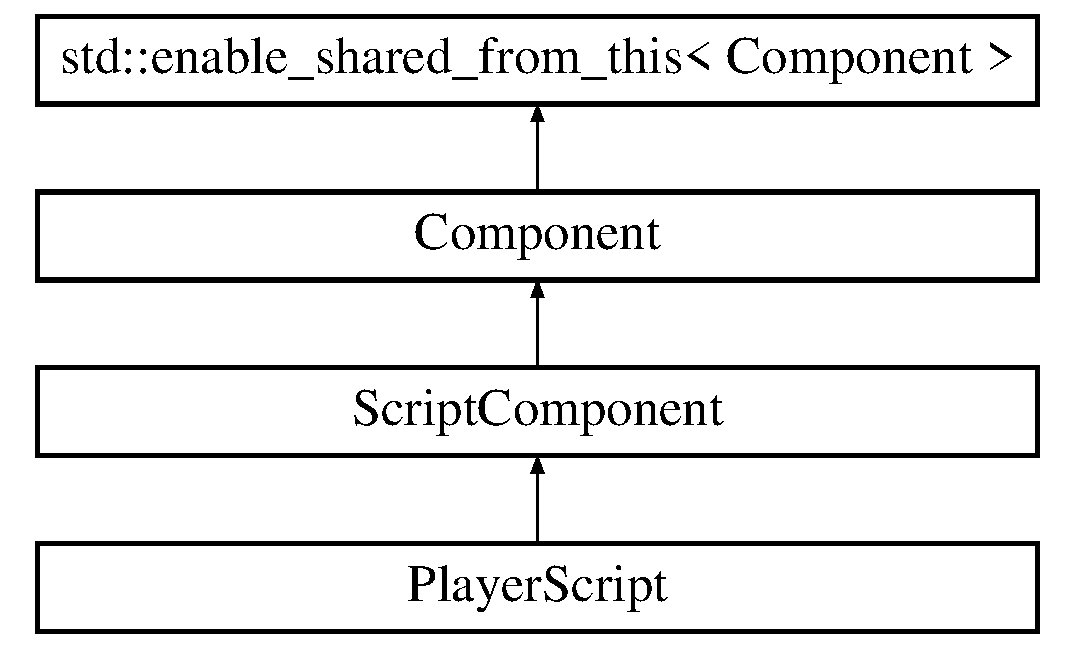
\includegraphics[height=4.000000cm]{class_player_script}
\end{center}
\end{figure}
\subsection*{Public Member Functions}
\begin{DoxyCompactItemize}
\item 
virtual void \hyperlink{class_player_script_acb623eb7cdcfc49b7848bf7d60809cb7}{awake} () override
\item 
virtual void \hyperlink{class_player_script_a5cd8853a54348831521f0455df5b508c}{tick} (float delta\+Secods) override
\item 
\hyperlink{class_player_script_a6fdee043545a61122b85536d2555d00c}{Player\+Script} ()
\item 
\hypertarget{class_player_script_a4d5b5edb9cf9bd82455631f8a08f32a5}{}void {\bfseries apply\+Drag} (float delta\+Seconds)\label{class_player_script_a4d5b5edb9cf9bd82455631f8a08f32a5}

\item 
virtual void \hyperlink{class_player_script_aa57ebbefa2e5be812b9a0272ae654258}{on\+Collision} (\hyperlink{class_actor}{Actor} $\ast$actor) override
\item 
virtual void \hyperlink{class_player_script_ad5476bdc3f1b168047def498cd62844f}{on\+Trigger} (\hyperlink{class_actor}{Actor} $\ast$actor) override
\item 
virtual shared\+\_\+ptr$<$ \hyperlink{class_component}{Component} $>$ \hyperlink{class_player_script_a75a83f06a2acb93ce1a629dcf2dabf5c}{clone} () override
\end{DoxyCompactItemize}
\subsection*{Public Attributes}
\begin{DoxyCompactItemize}
\item 
\hypertarget{class_player_script_ab3f3425c6c4e785c1b383372aa00cf2f}{}float {\bfseries move\+Speed}\label{class_player_script_ab3f3425c6c4e785c1b383372aa00cf2f}

\item 
\hypertarget{class_player_script_aa4c7eaaa33783dabfa9d78ca39ac711c}{}float {\bfseries rotate\+Speed}\label{class_player_script_aa4c7eaaa33783dabfa9d78ca39ac711c}

\item 
\hypertarget{class_player_script_a2f26a76ff6fbddb85a57271154e09c34}{}glm\+::vec3 {\bfseries velocity}\label{class_player_script_a2f26a76ff6fbddb85a57271154e09c34}

\item 
\hypertarget{class_player_script_a634f7d6cc4a865ba9f39c348f3d24554}{}weak\+\_\+ptr$<$ \hyperlink{class_actor}{Actor} $>$ {\bfseries actor}\label{class_player_script_a634f7d6cc4a865ba9f39c348f3d24554}

\item 
\hypertarget{class_player_script_ad9ef6dbd52d8b5b81225cd0c13120344}{}shared\+\_\+ptr$<$ \hyperlink{class_material}{Material} $>$ {\bfseries default\+Material\+Ref}\label{class_player_script_ad9ef6dbd52d8b5b81225cd0c13120344}

\item 
\hypertarget{class_player_script_a8d35b4540064e7b2e26b985a1b2db017}{}shared\+\_\+ptr$<$ \hyperlink{class_mesh}{Mesh} $>$ {\bfseries obj\+Mesh\+Ref}\label{class_player_script_a8d35b4540064e7b2e26b985a1b2db017}

\item 
\hypertarget{class_player_script_a78fce4a74b7e1e0875e407f5b8c4117b}{}weak\+\_\+ptr$<$ \hyperlink{class_actor}{Actor} $>$ {\bfseries bullet\+Spawn\+Point}\label{class_player_script_a78fce4a74b7e1e0875e407f5b8c4117b}

\end{DoxyCompactItemize}
\subsection*{Additional Inherited Members}


\subsection{Detailed Description}
Your documentation comment will go here 

\subsection{Constructor \& Destructor Documentation}
\hypertarget{class_player_script_a6fdee043545a61122b85536d2555d00c}{}\index{Player\+Script@{Player\+Script}!Player\+Script@{Player\+Script}}
\index{Player\+Script@{Player\+Script}!Player\+Script@{Player\+Script}}
\subsubsection[{Player\+Script()}]{\setlength{\rightskip}{0pt plus 5cm}Player\+Script\+::\+Player\+Script (
\begin{DoxyParamCaption}
{}
\end{DoxyParamCaption}
)}\label{class_player_script_a6fdee043545a61122b85536d2555d00c}
Your documentation comment will go here 

\subsection{Member Function Documentation}
\hypertarget{class_player_script_acb623eb7cdcfc49b7848bf7d60809cb7}{}\index{Player\+Script@{Player\+Script}!awake@{awake}}
\index{awake@{awake}!Player\+Script@{Player\+Script}}
\subsubsection[{awake() override}]{\setlength{\rightskip}{0pt plus 5cm}void Player\+Script\+::awake (
\begin{DoxyParamCaption}
{}
\end{DoxyParamCaption}
)\hspace{0.3cm}{\ttfamily [override]}, {\ttfamily [virtual]}}\label{class_player_script_acb623eb7cdcfc49b7848bf7d60809cb7}
\hyperlink{class_component}{Component} awake override 

Reimplemented from \hyperlink{class_script_component_a4667b8a3712e18b25cd6f49f12c5677d}{Script\+Component}.

\hypertarget{class_player_script_a75a83f06a2acb93ce1a629dcf2dabf5c}{}\index{Player\+Script@{Player\+Script}!clone@{clone}}
\index{clone@{clone}!Player\+Script@{Player\+Script}}
\subsubsection[{clone() override}]{\setlength{\rightskip}{0pt plus 5cm}shared\+\_\+ptr$<$ {\bf Component} $>$ Player\+Script\+::clone (
\begin{DoxyParamCaption}
{}
\end{DoxyParamCaption}
)\hspace{0.3cm}{\ttfamily [override]}, {\ttfamily [virtual]}}\label{class_player_script_a75a83f06a2acb93ce1a629dcf2dabf5c}
Clones current component (Prototype Design Pattern) \begin{DoxyReturn}{Returns}
shared\+\_\+ptr to cloned \hyperlink{class_script_component}{Script\+Component} \hyperlink{class_component}{Component} 
\end{DoxyReturn}


Reimplemented from \hyperlink{class_script_component_adebdf5187e8f41f68f445ff7555d5036}{Script\+Component}.

\hypertarget{class_player_script_aa57ebbefa2e5be812b9a0272ae654258}{}\index{Player\+Script@{Player\+Script}!on\+Collision@{on\+Collision}}
\index{on\+Collision@{on\+Collision}!Player\+Script@{Player\+Script}}
\subsubsection[{on\+Collision(\+Actor $\ast$actor) override}]{\setlength{\rightskip}{0pt plus 5cm}void Player\+Script\+::on\+Collision (
\begin{DoxyParamCaption}
\item[{{\bf Actor} $\ast$}]{actor}
\end{DoxyParamCaption}
)\hspace{0.3cm}{\ttfamily [override]}, {\ttfamily [virtual]}}\label{class_player_script_aa57ebbefa2e5be812b9a0272ae654258}
Callback function called when a collision occurs 

Reimplemented from \hyperlink{class_script_component_a9f84fa4e6c97f6b61926164c487fd6af}{Script\+Component}.

\hypertarget{class_player_script_ad5476bdc3f1b168047def498cd62844f}{}\index{Player\+Script@{Player\+Script}!on\+Trigger@{on\+Trigger}}
\index{on\+Trigger@{on\+Trigger}!Player\+Script@{Player\+Script}}
\subsubsection[{on\+Trigger(\+Actor $\ast$actor) override}]{\setlength{\rightskip}{0pt plus 5cm}void Player\+Script\+::on\+Trigger (
\begin{DoxyParamCaption}
\item[{{\bf Actor} $\ast$}]{actor}
\end{DoxyParamCaption}
)\hspace{0.3cm}{\ttfamily [override]}, {\ttfamily [virtual]}}\label{class_player_script_ad5476bdc3f1b168047def498cd62844f}
Callback function called when a trigger collision occurs 

Reimplemented from \hyperlink{class_script_component_a4632d59065aa53982b6b154d3bc60502}{Script\+Component}.

\hypertarget{class_player_script_a5cd8853a54348831521f0455df5b508c}{}\index{Player\+Script@{Player\+Script}!tick@{tick}}
\index{tick@{tick}!Player\+Script@{Player\+Script}}
\subsubsection[{tick(float delta\+Secods) override}]{\setlength{\rightskip}{0pt plus 5cm}void Player\+Script\+::tick (
\begin{DoxyParamCaption}
\item[{float}]{delta\+Secods}
\end{DoxyParamCaption}
)\hspace{0.3cm}{\ttfamily [override]}, {\ttfamily [virtual]}}\label{class_player_script_a5cd8853a54348831521f0455df5b508c}
\hyperlink{class_component}{Component} tick override 
\begin{DoxyParams}[1]{Parameters}
\mbox{\tt in}  & {\em delta\+Seconds} & last frame durations \\
\hline
\end{DoxyParams}


Reimplemented from \hyperlink{class_script_component_aa765fa62a343a8d83eb168d369b93a51}{Script\+Component}.



The documentation for this class was generated from the following files\+:\begin{DoxyCompactItemize}
\item 
/\+Users/guilherme\+\_\+cunha/\+Dev/\+G\+I\+T\+H\+U\+B/\+G\+U\+Inity/\+Source/Player\+Script.\+hpp\item 
/\+Users/guilherme\+\_\+cunha/\+Dev/\+G\+I\+T\+H\+U\+B/\+G\+U\+Inity/\+Source/Player\+Script.\+cpp\end{DoxyCompactItemize}

\hypertarget{class_pointer_holder}{}\section{Pointer\+Holder$<$ T $>$ Class Template Reference}
\label{class_pointer_holder}\index{Pointer\+Holder$<$ T $>$@{Pointer\+Holder$<$ T $>$}}
\subsection*{Public Member Functions}
\begin{DoxyCompactItemize}
\item 
\hypertarget{class_pointer_holder_a104637c9f641362bae3ab3a03046a3a9}{}{\bfseries Pointer\+Holder} (T $\ast$pointer)\label{class_pointer_holder_a104637c9f641362bae3ab3a03046a3a9}

\end{DoxyCompactItemize}
\subsection*{Public Attributes}
\begin{DoxyCompactItemize}
\item 
\hypertarget{class_pointer_holder_a1a482c769510b45b266b7ed1c99f89f9}{}T $\ast$ {\bfseries pointer}\label{class_pointer_holder_a1a482c769510b45b266b7ed1c99f89f9}

\end{DoxyCompactItemize}


The documentation for this class was generated from the following file\+:\begin{DoxyCompactItemize}
\item 
/\+Users/guilherme\+\_\+cunha/\+Dev/\+G\+I\+T\+H\+U\+B/\+G\+U\+Inity/\+Source/Pointer\+Holder.\+hpp\end{DoxyCompactItemize}

\hypertarget{class_ray}{}\section{Ray Class Reference}
\label{class_ray}\index{Ray@{Ray}}
\subsection*{Public Member Functions}
\begin{DoxyCompactItemize}
\item 
\hypertarget{class_ray_a49a2693e5f37e655a20ffcff69bb0b55}{}{\bfseries Ray} (glm\+::vec3 origin, glm\+::vec3 direction)\label{class_ray_a49a2693e5f37e655a20ffcff69bb0b55}

\item 
\hypertarget{class_ray_a09c2aa04dfe2732dc81ef09a39729b88}{}{\bfseries Ray} (\hyperlink{class_ray}{Ray} \&\&ray)\label{class_ray_a09c2aa04dfe2732dc81ef09a39729b88}

\end{DoxyCompactItemize}
\subsection*{Public Attributes}
\begin{DoxyCompactItemize}
\item 
\hypertarget{class_ray_af86f612d19416f116ad658c8f1a11e43}{}glm\+::vec3 {\bfseries origin}\label{class_ray_af86f612d19416f116ad658c8f1a11e43}

\item 
\hypertarget{class_ray_a6c8212513588a8f3a63b55eaf4e63c17}{}glm\+::vec3 {\bfseries direction}\label{class_ray_a6c8212513588a8f3a63b55eaf4e63c17}

\end{DoxyCompactItemize}


The documentation for this class was generated from the following files\+:\begin{DoxyCompactItemize}
\item 
/\+Users/guilherme\+\_\+cunha/\+Dev/\+G\+I\+T\+H\+U\+B/\+G\+U\+Inity/\+Source/Ray.\+hpp\item 
/\+Users/guilherme\+\_\+cunha/\+Dev/\+G\+I\+T\+H\+U\+B/\+G\+U\+Inity/\+Source/Ray.\+cpp\end{DoxyCompactItemize}

\hypertarget{class_rigid_body}{}\section{Rigid\+Body Class Reference}
\label{class_rigid_body}\index{Rigid\+Body@{Rigid\+Body}}


{\ttfamily \#include $<$Rigid\+Body.\+hpp$>$}

Inheritance diagram for Rigid\+Body\+:\begin{figure}[H]
\begin{center}
\leavevmode
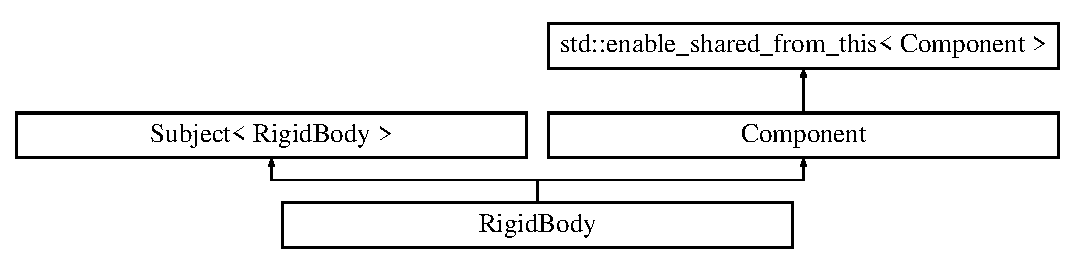
\includegraphics[height=3.000000cm]{class_rigid_body}
\end{center}
\end{figure}
\subsection*{Public Member Functions}
\begin{DoxyCompactItemize}
\item 
\hyperlink{class_rigid_body_a28203d38d278da0695ace20c66ee5f0a}{Rigid\+Body} ()
\item 
virtual \hyperlink{class_rigid_body_a4eade6e08e5a78c56822d2f42322c915}{$\sim$\+Rigid\+Body} ()
\item 
virtual void \hyperlink{class_rigid_body_aa419718573cb8042c3c7cbe671d69c4c}{init} () override
\item 
virtual void \hyperlink{class_rigid_body_a5ceba4a769ea558e5c7efd472e822248}{destroy} () override
\item 
virtual void \hyperlink{class_rigid_body_abf6a416e8bf2c2335bb2db145237ed4a}{tick} (float delta\+Secods) override
\item 
virtual void \hyperlink{class_rigid_body_a6f70cc83705a3a53b6ca3be6ff765a86}{set\+Active} (bool \hyperlink{class_component_a6dad4f819c0814eee8219e9b391cf583}{is\+Active}) override
\item 
Px\+Rigid\+Body $\ast$ \hyperlink{class_rigid_body_ab11c0e49a11a1521ed7124c9ea095368}{get\+Rigidbody} ()
\item 
void \hyperlink{class_rigid_body_a3272b6d18bc91c948fb6dadb2f7c1a39}{set\+Kinematic} (bool is\+Kinematic)
\item 
bool \hyperlink{class_rigid_body_ac93637a288e612654482eb8c75ce9d65}{get\+Kinematic} ()
\item 
void \hyperlink{class_rigid_body_af6c66756ca071aa93a64f604f7d2bc9a}{set\+Gravity} (bool enabled)
\item 
bool \hyperlink{class_rigid_body_af8caadbfee30eb55a2c408321544160f}{get\+Gravity} ()
\item 
void \hyperlink{class_rigid_body_a386d269dbc0e2584fa1c084c8eb86b08}{set\+Constraints\+Flags} (int constraint\+Flags)
\item 
int \hyperlink{class_rigid_body_aefe835ccb44041a78660d5a5241f412f}{get\+Constraints\+Flags} ()
\item 
void \hyperlink{class_rigid_body_a9401416338b535dd545002a5ba5e1f8e}{update\+Transform} (const Px\+Transform \&transform)
\item 
void \hyperlink{class_rigid_body_ac392797752276c328f0b0c00893ac3f1}{add\+Force} (glm\+::vec3 force)
\item 
virtual shared\+\_\+ptr$<$ \hyperlink{class_component}{Component} $>$ \hyperlink{class_rigid_body_a7acbed507a6deb5d83d381251ba224a8}{clone} () override
\item 
virtual shared\+\_\+ptr$<$ \hyperlink{class_component_description}{Component\+Description} $>$ \hyperlink{group__serialization__functions_ga0db7f5a90aa3397d0b3e0d2ae1ed1208}{get\+Component\+Description} () override
\item 
virtual void \hyperlink{group__serialization__functions_ga02c21f54650f36d529b4622efc9df372}{deserialize} (shared\+\_\+ptr$<$ \hyperlink{class_component_description}{Component\+Description} $>$ desc) override
\end{DoxyCompactItemize}
\subsection*{Additional Inherited Members}


\subsection{Detailed Description}
\hyperlink{class_rigid_body}{Rigid\+Body} is the component that adds real physics simulation to an \hyperlink{class_actor}{Actor}. It\textquotesingle{}s dynamic and directly influences in the \hyperlink{class_transform}{Transform} of the \hyperlink{class_actor}{Actor} due to physics simulation 

\subsection{Constructor \& Destructor Documentation}
\hypertarget{class_rigid_body_a28203d38d278da0695ace20c66ee5f0a}{}\index{Rigid\+Body@{Rigid\+Body}!Rigid\+Body@{Rigid\+Body}}
\index{Rigid\+Body@{Rigid\+Body}!Rigid\+Body@{Rigid\+Body}}
\subsubsection[{Rigid\+Body()}]{\setlength{\rightskip}{0pt plus 5cm}Rigid\+Body\+::\+Rigid\+Body (
\begin{DoxyParamCaption}
{}
\end{DoxyParamCaption}
)}\label{class_rigid_body_a28203d38d278da0695ace20c66ee5f0a}
Default Constructor \hypertarget{class_rigid_body_a4eade6e08e5a78c56822d2f42322c915}{}\index{Rigid\+Body@{Rigid\+Body}!````~Rigid\+Body@{$\sim$\+Rigid\+Body}}
\index{````~Rigid\+Body@{$\sim$\+Rigid\+Body}!Rigid\+Body@{Rigid\+Body}}
\subsubsection[{$\sim$\+Rigid\+Body()}]{\setlength{\rightskip}{0pt plus 5cm}Rigid\+Body\+::$\sim$\+Rigid\+Body (
\begin{DoxyParamCaption}
{}
\end{DoxyParamCaption}
)\hspace{0.3cm}{\ttfamily [virtual]}}\label{class_rigid_body_a4eade6e08e5a78c56822d2f42322c915}
Default Destructor 

\subsection{Member Function Documentation}
\hypertarget{class_rigid_body_ac392797752276c328f0b0c00893ac3f1}{}\index{Rigid\+Body@{Rigid\+Body}!add\+Force@{add\+Force}}
\index{add\+Force@{add\+Force}!Rigid\+Body@{Rigid\+Body}}
\subsubsection[{add\+Force(glm\+::vec3 force)}]{\setlength{\rightskip}{0pt plus 5cm}void Rigid\+Body\+::add\+Force (
\begin{DoxyParamCaption}
\item[{glm\+::vec3}]{axis}
\end{DoxyParamCaption}
)}\label{class_rigid_body_ac392797752276c328f0b0c00893ac3f1}
Add force to the \hyperlink{class_rigid_body}{Rigid\+Body} 
\begin{DoxyParams}[1]{Parameters}
\mbox{\tt in}  & {\em the} & force that will be added (direction and magnitude) \\
\hline
\end{DoxyParams}
\hypertarget{class_rigid_body_a7acbed507a6deb5d83d381251ba224a8}{}\index{Rigid\+Body@{Rigid\+Body}!clone@{clone}}
\index{clone@{clone}!Rigid\+Body@{Rigid\+Body}}
\subsubsection[{clone() override}]{\setlength{\rightskip}{0pt plus 5cm}shared\+\_\+ptr$<$ {\bf Component} $>$ Rigid\+Body\+::clone (
\begin{DoxyParamCaption}
{}
\end{DoxyParamCaption}
)\hspace{0.3cm}{\ttfamily [override]}, {\ttfamily [virtual]}}\label{class_rigid_body_a7acbed507a6deb5d83d381251ba224a8}
Clones current component (Prototype Design Pattern) \begin{DoxyReturn}{Returns}
shared\+\_\+ptr to cloned \hyperlink{class_rigid_body}{Rigid\+Body} \hyperlink{class_component}{Component} 
\end{DoxyReturn}


Implements \hyperlink{class_component_a74c984bd819bbef16fd4f306a90d34fe}{Component}.

\hypertarget{class_rigid_body_a5ceba4a769ea558e5c7efd472e822248}{}\index{Rigid\+Body@{Rigid\+Body}!destroy@{destroy}}
\index{destroy@{destroy}!Rigid\+Body@{Rigid\+Body}}
\subsubsection[{destroy() override}]{\setlength{\rightskip}{0pt plus 5cm}void Rigid\+Body\+::destroy (
\begin{DoxyParamCaption}
{}
\end{DoxyParamCaption}
)\hspace{0.3cm}{\ttfamily [override]}, {\ttfamily [virtual]}}\label{class_rigid_body_a5ceba4a769ea558e5c7efd472e822248}
\hyperlink{class_component}{Component} destroy override. Releases the Rigid\+Dynamic body 

Reimplemented from \hyperlink{class_component_a77b8fff56ddce5dd0b4a9dabb0b5202b}{Component}.

\hypertarget{class_rigid_body_aefe835ccb44041a78660d5a5241f412f}{}\index{Rigid\+Body@{Rigid\+Body}!get\+Constraints\+Flags@{get\+Constraints\+Flags}}
\index{get\+Constraints\+Flags@{get\+Constraints\+Flags}!Rigid\+Body@{Rigid\+Body}}
\subsubsection[{get\+Constraints\+Flags()}]{\setlength{\rightskip}{0pt plus 5cm}int Rigid\+Body\+::get\+Constraints\+Flags (
\begin{DoxyParamCaption}
{}
\end{DoxyParamCaption}
)}\label{class_rigid_body_aefe835ccb44041a78660d5a5241f412f}
Set the translation/rotation constraints of the rigidbody. \begin{DoxyReturn}{Returns}
current constraints of the rigidbody s 
\end{DoxyReturn}
\hypertarget{class_rigid_body_af8caadbfee30eb55a2c408321544160f}{}\index{Rigid\+Body@{Rigid\+Body}!get\+Gravity@{get\+Gravity}}
\index{get\+Gravity@{get\+Gravity}!Rigid\+Body@{Rigid\+Body}}
\subsubsection[{get\+Gravity()}]{\setlength{\rightskip}{0pt plus 5cm}bool Rigid\+Body\+::get\+Gravity (
\begin{DoxyParamCaption}
{}
\end{DoxyParamCaption}
)}\label{class_rigid_body_af8caadbfee30eb55a2c408321544160f}
gravity getter \begin{DoxyReturn}{Returns}
true if gravity is enabled, false otherwise 
\end{DoxyReturn}
\hypertarget{class_rigid_body_ac93637a288e612654482eb8c75ce9d65}{}\index{Rigid\+Body@{Rigid\+Body}!get\+Kinematic@{get\+Kinematic}}
\index{get\+Kinematic@{get\+Kinematic}!Rigid\+Body@{Rigid\+Body}}
\subsubsection[{get\+Kinematic()}]{\setlength{\rightskip}{0pt plus 5cm}bool Rigid\+Body\+::get\+Kinematic (
\begin{DoxyParamCaption}
{}
\end{DoxyParamCaption}
)}\label{class_rigid_body_ac93637a288e612654482eb8c75ce9d65}
is\+Kinematic getter \begin{DoxyReturn}{Returns}
true if physics is being simulated, false if it\textquotesingle{}s not 
\end{DoxyReturn}
\hypertarget{class_rigid_body_ab11c0e49a11a1521ed7124c9ea095368}{}\index{Rigid\+Body@{Rigid\+Body}!get\+Rigidbody@{get\+Rigidbody}}
\index{get\+Rigidbody@{get\+Rigidbody}!Rigid\+Body@{Rigid\+Body}}
\subsubsection[{get\+Rigidbody()}]{\setlength{\rightskip}{0pt plus 5cm}Px\+Rigid\+Body $\ast$ Rigid\+Body\+::get\+Rigidbody (
\begin{DoxyParamCaption}
{}
\end{DoxyParamCaption}
)}\label{class_rigid_body_ab11c0e49a11a1521ed7124c9ea095368}
physx\+Rigid\+Body getter \begin{DoxyReturn}{Returns}
pointer to Phys\+X \hyperlink{class_rigid_body}{Rigid\+Body} 
\end{DoxyReturn}
\hypertarget{class_rigid_body_aa419718573cb8042c3c7cbe671d69c4c}{}\index{Rigid\+Body@{Rigid\+Body}!init@{init}}
\index{init@{init}!Rigid\+Body@{Rigid\+Body}}
\subsubsection[{init() override}]{\setlength{\rightskip}{0pt plus 5cm}void Rigid\+Body\+::init (
\begin{DoxyParamCaption}
{}
\end{DoxyParamCaption}
)\hspace{0.3cm}{\ttfamily [override]}, {\ttfamily [virtual]}}\label{class_rigid_body_aa419718573cb8042c3c7cbe671d69c4c}
\hyperlink{class_component}{Component} init override. Creates a Rigid\+Dynamic body in the Phys\+X scene 

Reimplemented from \hyperlink{class_component_a162f8cdc070537a71f2ad0b5e763b86f}{Component}.

\hypertarget{class_rigid_body_a6f70cc83705a3a53b6ca3be6ff765a86}{}\index{Rigid\+Body@{Rigid\+Body}!set\+Active@{set\+Active}}
\index{set\+Active@{set\+Active}!Rigid\+Body@{Rigid\+Body}}
\subsubsection[{set\+Active(bool is\+Active) override}]{\setlength{\rightskip}{0pt plus 5cm}void Rigid\+Body\+::set\+Active (
\begin{DoxyParamCaption}
\item[{bool}]{is\+Active}
\end{DoxyParamCaption}
)\hspace{0.3cm}{\ttfamily [override]}, {\ttfamily [virtual]}}\label{class_rigid_body_a6f70cc83705a3a53b6ca3be6ff765a86}
\hyperlink{class_component}{Component} set\+Active override. Disables visualization and physics simulation in the Phys\+X scene 

Reimplemented from \hyperlink{class_component}{Component}.

\hypertarget{class_rigid_body_a386d269dbc0e2584fa1c084c8eb86b08}{}\index{Rigid\+Body@{Rigid\+Body}!set\+Constraints\+Flags@{set\+Constraints\+Flags}}
\index{set\+Constraints\+Flags@{set\+Constraints\+Flags}!Rigid\+Body@{Rigid\+Body}}
\subsubsection[{set\+Constraints\+Flags(int constraint\+Flags)}]{\setlength{\rightskip}{0pt plus 5cm}void Rigid\+Body\+::set\+Constraints\+Flags (
\begin{DoxyParamCaption}
\item[{int}]{constraint\+Flags}
\end{DoxyParamCaption}
)}\label{class_rigid_body_a386d269dbc0e2584fa1c084c8eb86b08}
Set the translation/rotation constraints of the rigidbody. 
\begin{DoxyParams}[1]{Parameters}
\mbox{\tt in}  & {\em flags} & to constrain \\
\hline
\end{DoxyParams}
\hypertarget{class_rigid_body_af6c66756ca071aa93a64f604f7d2bc9a}{}\index{Rigid\+Body@{Rigid\+Body}!set\+Gravity@{set\+Gravity}}
\index{set\+Gravity@{set\+Gravity}!Rigid\+Body@{Rigid\+Body}}
\subsubsection[{set\+Gravity(bool enabled)}]{\setlength{\rightskip}{0pt plus 5cm}void Rigid\+Body\+::set\+Gravity (
\begin{DoxyParamCaption}
\item[{bool}]{enabled}
\end{DoxyParamCaption}
)}\label{class_rigid_body_af6c66756ca071aa93a64f604f7d2bc9a}
gravity setter 
\begin{DoxyParams}[1]{Parameters}
\mbox{\tt in}  & {\em enabled} & true if gravity is enabled, false otherwise \\
\hline
\end{DoxyParams}
\hypertarget{class_rigid_body_a3272b6d18bc91c948fb6dadb2f7c1a39}{}\index{Rigid\+Body@{Rigid\+Body}!set\+Kinematic@{set\+Kinematic}}
\index{set\+Kinematic@{set\+Kinematic}!Rigid\+Body@{Rigid\+Body}}
\subsubsection[{set\+Kinematic(bool is\+Kinematic)}]{\setlength{\rightskip}{0pt plus 5cm}void Rigid\+Body\+::set\+Kinematic (
\begin{DoxyParamCaption}
\item[{bool}]{is\+Kinematic}
\end{DoxyParamCaption}
)}\label{class_rigid_body_a3272b6d18bc91c948fb6dadb2f7c1a39}
is\+Kinematic setter 
\begin{DoxyParams}{Parameters}
{\em true} & if physics should be not be simulated, false if it should \\
\hline
\end{DoxyParams}
\hypertarget{class_rigid_body_abf6a416e8bf2c2335bb2db145237ed4a}{}\index{Rigid\+Body@{Rigid\+Body}!tick@{tick}}
\index{tick@{tick}!Rigid\+Body@{Rigid\+Body}}
\subsubsection[{tick(float delta\+Secods) override}]{\setlength{\rightskip}{0pt plus 5cm}void Rigid\+Body\+::tick (
\begin{DoxyParamCaption}
\item[{float}]{delta\+Seconds}
\end{DoxyParamCaption}
)\hspace{0.3cm}{\ttfamily [override]}, {\ttfamily [virtual]}}\label{class_rigid_body_abf6a416e8bf2c2335bb2db145237ed4a}
\hyperlink{class_component}{Component} tick override. Updates the Phys\+X scene with the \hyperlink{class_actor}{Actor} transform 
\begin{DoxyParams}[1]{Parameters}
\mbox{\tt in}  & {\em delta\+Seconds} & last frame duration\\
\hline
\end{DoxyParams}
\hyperlink{class_component}{Component} tick override. Updates the Phys\+X scene with the \hyperlink{class_actor}{Actor} transform 

Reimplemented from \hyperlink{class_component_a72d67b02e6733c1a6fb73cbaaf8ebff4}{Component}.

\hypertarget{class_rigid_body_a9401416338b535dd545002a5ba5e1f8e}{}\index{Rigid\+Body@{Rigid\+Body}!update\+Transform@{update\+Transform}}
\index{update\+Transform@{update\+Transform}!Rigid\+Body@{Rigid\+Body}}
\subsubsection[{update\+Transform(const Px\+Transform \&transform)}]{\setlength{\rightskip}{0pt plus 5cm}void Rigid\+Body\+::update\+Transform (
\begin{DoxyParamCaption}
\item[{const Px\+Transform \&}]{new\+Transform}
\end{DoxyParamCaption}
)}\label{class_rigid_body_a9401416338b535dd545002a5ba5e1f8e}
Update the transform based on the Phys\+X physics simulation and current constraints 
\begin{DoxyParams}[1]{Parameters}
\mbox{\tt in}  & {\em the} & Phys\+X transform \\
\hline
\end{DoxyParams}


The documentation for this class was generated from the following files\+:\begin{DoxyCompactItemize}
\item 
/\+Users/guilherme\+\_\+cunha/\+Dev/\+G\+I\+T\+H\+U\+B/\+G\+U\+Inity/\+Source/Rigid\+Body.\+hpp\item 
/\+Users/guilherme\+\_\+cunha/\+Dev/\+G\+I\+T\+H\+U\+B/\+G\+U\+Inity/\+Source/Rigid\+Body.\+cpp\end{DoxyCompactItemize}

\hypertarget{class_rigid_body_description}{}\section{Rigid\+Body\+Description Class Reference}
\label{class_rigid_body_description}\index{Rigid\+Body\+Description@{Rigid\+Body\+Description}}
Inheritance diagram for Rigid\+Body\+Description\+:\begin{figure}[H]
\begin{center}
\leavevmode
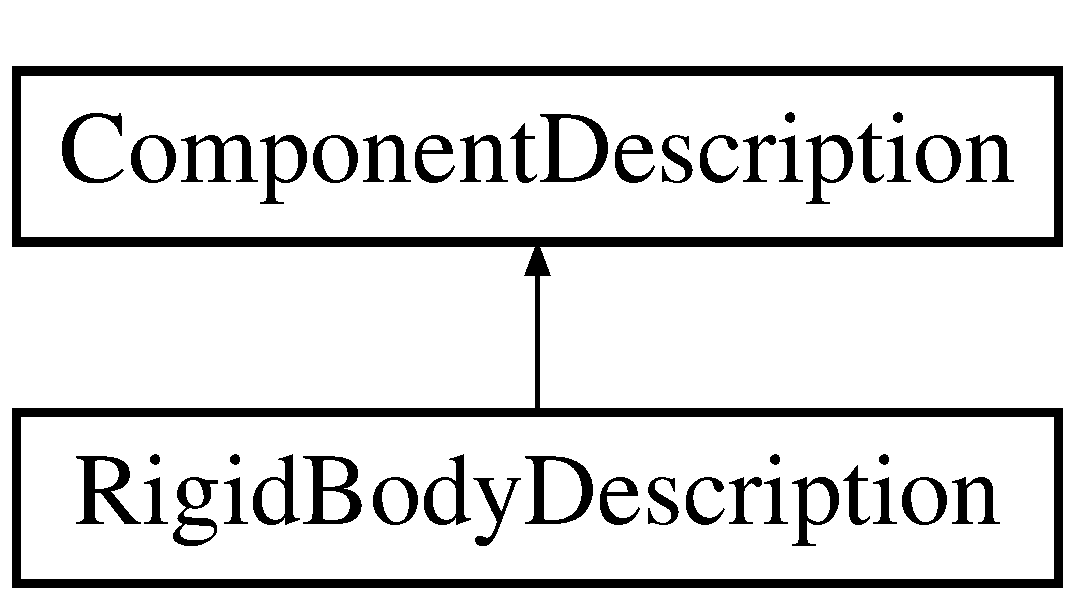
\includegraphics[height=2.000000cm]{class_rigid_body_description}
\end{center}
\end{figure}
\subsection*{Public Member Functions}
\begin{DoxyCompactItemize}
\item 
\hypertarget{class_rigid_body_description_a1c0f0ca31631e710b319e6e641f153f0}{}{\bfseries Rigid\+Body\+Description} (bool kinematic)\label{class_rigid_body_description_a1c0f0ca31631e710b319e6e641f153f0}

\end{DoxyCompactItemize}
\subsection*{Public Attributes}
\begin{DoxyCompactItemize}
\item 
\hypertarget{class_rigid_body_description_ae14f3e10a9888a4906638864c7a2ad3c}{}bool {\bfseries is\+Kinematic}\label{class_rigid_body_description_ae14f3e10a9888a4906638864c7a2ad3c}

\end{DoxyCompactItemize}


The documentation for this class was generated from the following file\+:\begin{DoxyCompactItemize}
\item 
/\+Users/guilherme\+\_\+cunha/\+Dev/\+G\+I\+T\+H\+U\+B/\+G\+U\+Inity/\+Source/Serialization\+Structs.\+hpp\end{DoxyCompactItemize}

\hypertarget{class_rigid_static}{}\section{Rigid\+Static Class Reference}
\label{class_rigid_static}\index{Rigid\+Static@{Rigid\+Static}}


{\ttfamily \#include $<$Rigid\+Static.\+hpp$>$}

Inheritance diagram for Rigid\+Static\+:\begin{figure}[H]
\begin{center}
\leavevmode
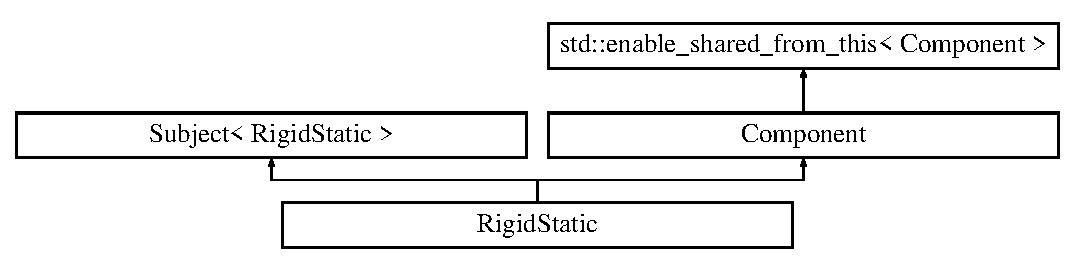
\includegraphics[height=3.000000cm]{class_rigid_static}
\end{center}
\end{figure}
\subsection*{Public Member Functions}
\begin{DoxyCompactItemize}
\item 
\hyperlink{class_rigid_static_ae2a704e78025e8b938939153b24c5548}{Rigid\+Static} ()
\item 
virtual \hyperlink{class_rigid_static_a66a806674d933319ab77d39315a998b5}{$\sim$\+Rigid\+Static} ()
\item 
virtual void \hyperlink{class_rigid_static_a2844109f1ef8fe36a25ce065934d703c}{init} () override
\item 
virtual void \hyperlink{class_rigid_static_abd99e84cc884043d5afde1b95fb0d3b3}{destroy} () override
\item 
virtual void \hyperlink{class_rigid_static_a3eef6474e9396db05dc714e41154e793}{tick} (float delta\+Secods) override
\item 
virtual void \hyperlink{class_rigid_static_a439d621f3b44b8da9fc17faf88635267}{set\+Active} (bool \hyperlink{class_component_a6dad4f819c0814eee8219e9b391cf583}{is\+Active}) override
\item 
Px\+Rigid\+Dynamic $\ast$ \hyperlink{class_rigid_static_ab7734d16020ce18dee3c96a2010fa7b8}{get\+Rigid\+Dynamic} ()
\item 
virtual shared\+\_\+ptr$<$ \hyperlink{class_component}{Component} $>$ \hyperlink{class_rigid_static_a5fef27a8ca3f6e969fb4c8312c1bba0a}{clone} () override
\item 
virtual shared\+\_\+ptr$<$ \hyperlink{class_component_description}{Component\+Description} $>$ \hyperlink{group__serialization__functions_ga74f14a6073ed781cc12f42c0a936515a}{get\+Component\+Description} () override
\item 
virtual void \hyperlink{group__serialization__functions_ga80ddd737e7b8b80a997a0c6681925a26}{deserialize} (shared\+\_\+ptr$<$ \hyperlink{class_component_description}{Component\+Description} $>$ desc) override
\end{DoxyCompactItemize}
\subsection*{Additional Inherited Members}


\subsection{Detailed Description}
\hyperlink{class_rigid_static}{Rigid\+Static} is the component that adds real physics simulation to an \hyperlink{class_actor}{Actor}. It\textquotesingle{}s static and can be moved by the \hyperlink{class_game}{Game} but will never be moved due to physics simulation 

\subsection{Constructor \& Destructor Documentation}
\hypertarget{class_rigid_static_ae2a704e78025e8b938939153b24c5548}{}\index{Rigid\+Static@{Rigid\+Static}!Rigid\+Static@{Rigid\+Static}}
\index{Rigid\+Static@{Rigid\+Static}!Rigid\+Static@{Rigid\+Static}}
\subsubsection[{Rigid\+Static()}]{\setlength{\rightskip}{0pt plus 5cm}Rigid\+Static\+::\+Rigid\+Static (
\begin{DoxyParamCaption}
{}
\end{DoxyParamCaption}
)}\label{class_rigid_static_ae2a704e78025e8b938939153b24c5548}
Default Constructor \hypertarget{class_rigid_static_a66a806674d933319ab77d39315a998b5}{}\index{Rigid\+Static@{Rigid\+Static}!````~Rigid\+Static@{$\sim$\+Rigid\+Static}}
\index{````~Rigid\+Static@{$\sim$\+Rigid\+Static}!Rigid\+Static@{Rigid\+Static}}
\subsubsection[{$\sim$\+Rigid\+Static()}]{\setlength{\rightskip}{0pt plus 5cm}Rigid\+Static\+::$\sim$\+Rigid\+Static (
\begin{DoxyParamCaption}
{}
\end{DoxyParamCaption}
)\hspace{0.3cm}{\ttfamily [virtual]}}\label{class_rigid_static_a66a806674d933319ab77d39315a998b5}
Default Destructor 

\subsection{Member Function Documentation}
\hypertarget{class_rigid_static_a5fef27a8ca3f6e969fb4c8312c1bba0a}{}\index{Rigid\+Static@{Rigid\+Static}!clone@{clone}}
\index{clone@{clone}!Rigid\+Static@{Rigid\+Static}}
\subsubsection[{clone() override}]{\setlength{\rightskip}{0pt plus 5cm}shared\+\_\+ptr$<$ {\bf Component} $>$ Rigid\+Static\+::clone (
\begin{DoxyParamCaption}
{}
\end{DoxyParamCaption}
)\hspace{0.3cm}{\ttfamily [override]}, {\ttfamily [virtual]}}\label{class_rigid_static_a5fef27a8ca3f6e969fb4c8312c1bba0a}
Clones current component (Prototype Design Pattern) \begin{DoxyReturn}{Returns}
shared\+\_\+ptr to cloned \hyperlink{class_rigid_static}{Rigid\+Static} \hyperlink{class_component}{Component} 
\end{DoxyReturn}


Implements \hyperlink{class_component_a74c984bd819bbef16fd4f306a90d34fe}{Component}.

\hypertarget{class_rigid_static_abd99e84cc884043d5afde1b95fb0d3b3}{}\index{Rigid\+Static@{Rigid\+Static}!destroy@{destroy}}
\index{destroy@{destroy}!Rigid\+Static@{Rigid\+Static}}
\subsubsection[{destroy() override}]{\setlength{\rightskip}{0pt plus 5cm}void Rigid\+Static\+::destroy (
\begin{DoxyParamCaption}
{}
\end{DoxyParamCaption}
)\hspace{0.3cm}{\ttfamily [override]}, {\ttfamily [virtual]}}\label{class_rigid_static_abd99e84cc884043d5afde1b95fb0d3b3}
\hyperlink{class_component}{Component} destroy override. Releases the Rigid\+Dynamic body 

Reimplemented from \hyperlink{class_component_a77b8fff56ddce5dd0b4a9dabb0b5202b}{Component}.

\hypertarget{class_rigid_static_ab7734d16020ce18dee3c96a2010fa7b8}{}\index{Rigid\+Static@{Rigid\+Static}!get\+Rigid\+Dynamic@{get\+Rigid\+Dynamic}}
\index{get\+Rigid\+Dynamic@{get\+Rigid\+Dynamic}!Rigid\+Static@{Rigid\+Static}}
\subsubsection[{get\+Rigid\+Dynamic()}]{\setlength{\rightskip}{0pt plus 5cm}Px\+Rigid\+Dynamic $\ast$ Rigid\+Static\+::get\+Rigid\+Dynamic (
\begin{DoxyParamCaption}
{}
\end{DoxyParamCaption}
)}\label{class_rigid_static_ab7734d16020ce18dee3c96a2010fa7b8}
physx\+Rigid\+Body getter \begin{DoxyReturn}{Returns}
pointer to Phys\+X \hyperlink{class_rigid_body}{Rigid\+Body} 
\end{DoxyReturn}
\hypertarget{class_rigid_static_a2844109f1ef8fe36a25ce065934d703c}{}\index{Rigid\+Static@{Rigid\+Static}!init@{init}}
\index{init@{init}!Rigid\+Static@{Rigid\+Static}}
\subsubsection[{init() override}]{\setlength{\rightskip}{0pt plus 5cm}void Rigid\+Static\+::init (
\begin{DoxyParamCaption}
{}
\end{DoxyParamCaption}
)\hspace{0.3cm}{\ttfamily [override]}, {\ttfamily [virtual]}}\label{class_rigid_static_a2844109f1ef8fe36a25ce065934d703c}
\hyperlink{class_component}{Component} init override. Creates a Rigid\+Dynamic body in the Phys\+X scene and sets it as Kinematic by default 

Reimplemented from \hyperlink{class_component_a162f8cdc070537a71f2ad0b5e763b86f}{Component}.

\hypertarget{class_rigid_static_a439d621f3b44b8da9fc17faf88635267}{}\index{Rigid\+Static@{Rigid\+Static}!set\+Active@{set\+Active}}
\index{set\+Active@{set\+Active}!Rigid\+Static@{Rigid\+Static}}
\subsubsection[{set\+Active(bool is\+Active) override}]{\setlength{\rightskip}{0pt plus 5cm}void Rigid\+Static\+::set\+Active (
\begin{DoxyParamCaption}
\item[{bool}]{is\+Active}
\end{DoxyParamCaption}
)\hspace{0.3cm}{\ttfamily [override]}, {\ttfamily [virtual]}}\label{class_rigid_static_a439d621f3b44b8da9fc17faf88635267}
\hyperlink{class_component}{Component} set\+Active override. Disables visualization and physics simulation in the Phys\+X scene 

Reimplemented from \hyperlink{class_component}{Component}.

\hypertarget{class_rigid_static_a3eef6474e9396db05dc714e41154e793}{}\index{Rigid\+Static@{Rigid\+Static}!tick@{tick}}
\index{tick@{tick}!Rigid\+Static@{Rigid\+Static}}
\subsubsection[{tick(float delta\+Secods) override}]{\setlength{\rightskip}{0pt plus 5cm}void Rigid\+Static\+::tick (
\begin{DoxyParamCaption}
\item[{float}]{delta\+Seconds}
\end{DoxyParamCaption}
)\hspace{0.3cm}{\ttfamily [override]}, {\ttfamily [virtual]}}\label{class_rigid_static_a3eef6474e9396db05dc714e41154e793}
\hyperlink{class_component}{Component} tick override. Updates the Phys\+X scene with the \hyperlink{class_actor}{Actor} transform 
\begin{DoxyParams}[1]{Parameters}
\mbox{\tt in}  & {\em delta\+Seconds} & last frame duration \\
\hline
\end{DoxyParams}


Reimplemented from \hyperlink{class_component_a72d67b02e6733c1a6fb73cbaaf8ebff4}{Component}.



The documentation for this class was generated from the following files\+:\begin{DoxyCompactItemize}
\item 
/\+Users/guilherme\+\_\+cunha/\+Dev/\+G\+I\+T\+H\+U\+B/\+G\+U\+Inity/\+Source/Rigid\+Static.\+hpp\item 
/\+Users/guilherme\+\_\+cunha/\+Dev/\+G\+I\+T\+H\+U\+B/\+G\+U\+Inity/\+Source/Rigid\+Static.\+cpp\end{DoxyCompactItemize}

\hypertarget{class_rigid_static_description}{}\section{Rigid\+Static\+Description Class Reference}
\label{class_rigid_static_description}\index{Rigid\+Static\+Description@{Rigid\+Static\+Description}}
Inheritance diagram for Rigid\+Static\+Description\+:\begin{figure}[H]
\begin{center}
\leavevmode
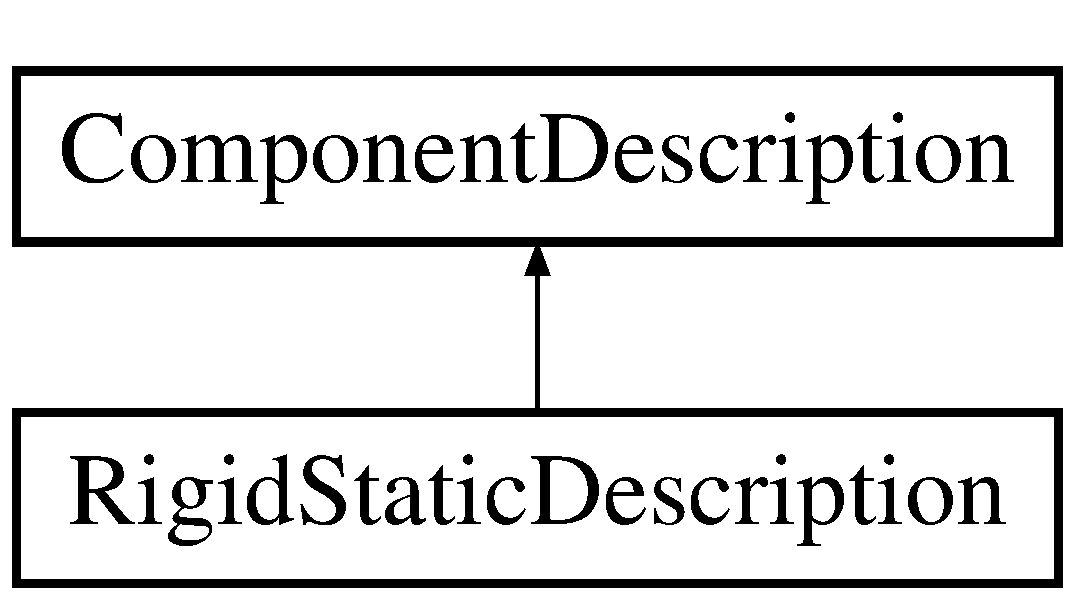
\includegraphics[height=2.000000cm]{class_rigid_static_description}
\end{center}
\end{figure}
\subsection*{Additional Inherited Members}


The documentation for this class was generated from the following file\+:\begin{DoxyCompactItemize}
\item 
/\+Users/guilherme\+\_\+cunha/\+Dev/\+G\+I\+T\+H\+U\+B/\+G\+U\+Inity/\+Source/Serialization\+Structs.\+hpp\end{DoxyCompactItemize}

\hypertarget{class_rotate_handle}{}\section{Rotate\+Handle Class Reference}
\label{class_rotate_handle}\index{Rotate\+Handle@{Rotate\+Handle}}
Inheritance diagram for Rotate\+Handle\+:\begin{figure}[H]
\begin{center}
\leavevmode
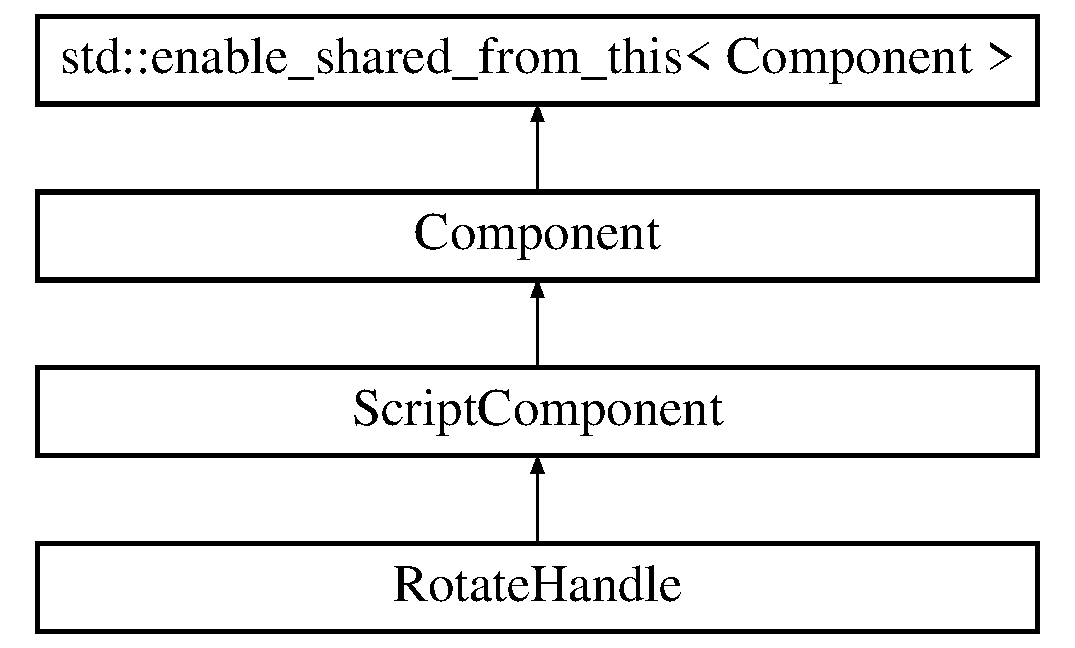
\includegraphics[height=4.000000cm]{class_rotate_handle}
\end{center}
\end{figure}
\subsection*{Public Member Functions}
\begin{DoxyCompactItemize}
\item 
\hypertarget{class_rotate_handle_ac3e55cbbed2ffd3914e5012f9075551d}{}void {\bfseries set\+Axis} (Rotate\+Axis axis)\label{class_rotate_handle_ac3e55cbbed2ffd3914e5012f9075551d}

\item 
virtual void \hyperlink{class_rotate_handle_a93caa7dd2992d5dc3fcef9cbc4278bed}{awake} () override
\item 
virtual void \hyperlink{class_rotate_handle_a58b0a9ebbcd28378aed805628107eef4}{tick} (float delta\+Seconds) override
\end{DoxyCompactItemize}
\subsection*{Public Attributes}
\begin{DoxyCompactItemize}
\item 
\hypertarget{class_rotate_handle_aabd470e68ebdb6e8f17f55041d952a1f}{}Rotate\+Axis {\bfseries axis}\label{class_rotate_handle_aabd470e68ebdb6e8f17f55041d952a1f}

\end{DoxyCompactItemize}
\subsection*{Additional Inherited Members}


\subsection{Member Function Documentation}
\hypertarget{class_rotate_handle_a93caa7dd2992d5dc3fcef9cbc4278bed}{}\index{Rotate\+Handle@{Rotate\+Handle}!awake@{awake}}
\index{awake@{awake}!Rotate\+Handle@{Rotate\+Handle}}
\subsubsection[{awake() override}]{\setlength{\rightskip}{0pt plus 5cm}void Rotate\+Handle\+::awake (
\begin{DoxyParamCaption}
{}
\end{DoxyParamCaption}
)\hspace{0.3cm}{\ttfamily [override]}, {\ttfamily [virtual]}}\label{class_rotate_handle_a93caa7dd2992d5dc3fcef9cbc4278bed}
\hyperlink{class_component}{Component} awake override 

Reimplemented from \hyperlink{class_script_component_a4667b8a3712e18b25cd6f49f12c5677d}{Script\+Component}.

\hypertarget{class_rotate_handle_a58b0a9ebbcd28378aed805628107eef4}{}\index{Rotate\+Handle@{Rotate\+Handle}!tick@{tick}}
\index{tick@{tick}!Rotate\+Handle@{Rotate\+Handle}}
\subsubsection[{tick(float delta\+Seconds) override}]{\setlength{\rightskip}{0pt plus 5cm}void Rotate\+Handle\+::tick (
\begin{DoxyParamCaption}
\item[{float}]{delta\+Secods}
\end{DoxyParamCaption}
)\hspace{0.3cm}{\ttfamily [override]}, {\ttfamily [virtual]}}\label{class_rotate_handle_a58b0a9ebbcd28378aed805628107eef4}
\hyperlink{class_component}{Component} tick override 
\begin{DoxyParams}[1]{Parameters}
\mbox{\tt in}  & {\em delta\+Seconds} & last frame durations \\
\hline
\end{DoxyParams}


Reimplemented from \hyperlink{class_script_component_aa765fa62a343a8d83eb168d369b93a51}{Script\+Component}.



The documentation for this class was generated from the following files\+:\begin{DoxyCompactItemize}
\item 
/\+Users/guilherme\+\_\+cunha/\+Dev/\+G\+I\+T\+H\+U\+B/\+G\+U\+Inity/\+Source/Rotate\+Handle.\+hpp\item 
/\+Users/guilherme\+\_\+cunha/\+Dev/\+G\+I\+T\+H\+U\+B/\+G\+U\+Inity/\+Source/Rotate\+Handle.\+cpp\end{DoxyCompactItemize}

\hypertarget{class_rotate_over_time}{}\section{Rotate\+Over\+Time Class Reference}
\label{class_rotate_over_time}\index{Rotate\+Over\+Time@{Rotate\+Over\+Time}}
Inheritance diagram for Rotate\+Over\+Time\+:\begin{figure}[H]
\begin{center}
\leavevmode
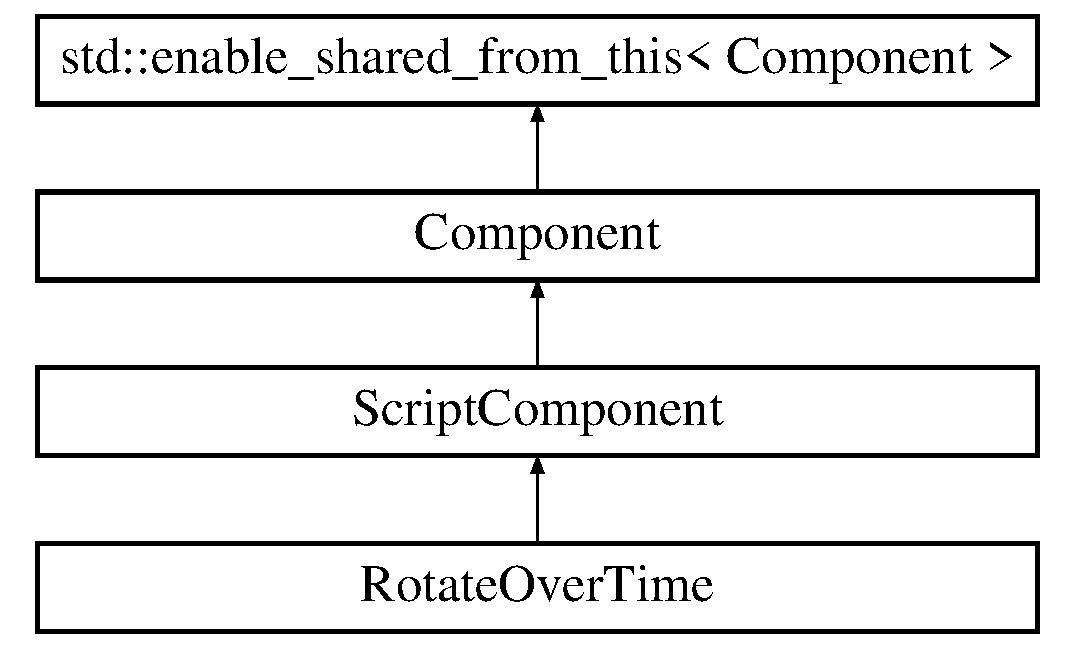
\includegraphics[height=4.000000cm]{class_rotate_over_time}
\end{center}
\end{figure}
\subsection*{Public Member Functions}
\begin{DoxyCompactItemize}
\item 
void \hyperlink{class_rotate_over_time_a57f0412df19fefd4ab4dd11839c483e1}{tick} (float delta\+Seconds) override
\end{DoxyCompactItemize}
\subsection*{Additional Inherited Members}


\subsection{Member Function Documentation}
\hypertarget{class_rotate_over_time_a57f0412df19fefd4ab4dd11839c483e1}{}\index{Rotate\+Over\+Time@{Rotate\+Over\+Time}!tick@{tick}}
\index{tick@{tick}!Rotate\+Over\+Time@{Rotate\+Over\+Time}}
\subsubsection[{tick(float delta\+Seconds) override}]{\setlength{\rightskip}{0pt plus 5cm}void Rotate\+Over\+Time\+::tick (
\begin{DoxyParamCaption}
\item[{float}]{delta\+Secods}
\end{DoxyParamCaption}
)\hspace{0.3cm}{\ttfamily [override]}, {\ttfamily [virtual]}}\label{class_rotate_over_time_a57f0412df19fefd4ab4dd11839c483e1}
\hyperlink{class_component}{Component} tick override 
\begin{DoxyParams}[1]{Parameters}
\mbox{\tt in}  & {\em delta\+Seconds} & last frame durations \\
\hline
\end{DoxyParams}


Reimplemented from \hyperlink{class_script_component_aa765fa62a343a8d83eb168d369b93a51}{Script\+Component}.



The documentation for this class was generated from the following files\+:\begin{DoxyCompactItemize}
\item 
/\+Users/guilherme\+\_\+cunha/\+Dev/\+G\+I\+T\+H\+U\+B/\+G\+U\+Inity/\+Source/Rotate\+Over\+Time.\+hpp\item 
/\+Users/guilherme\+\_\+cunha/\+Dev/\+G\+I\+T\+H\+U\+B/\+G\+U\+Inity/\+Source/Rotate\+Over\+Time.\+cpp\end{DoxyCompactItemize}

\hypertarget{class_rotate_tool}{}\section{Rotate\+Tool Class Reference}
\label{class_rotate_tool}\index{Rotate\+Tool@{Rotate\+Tool}}
Inheritance diagram for Rotate\+Tool\+:\begin{figure}[H]
\begin{center}
\leavevmode
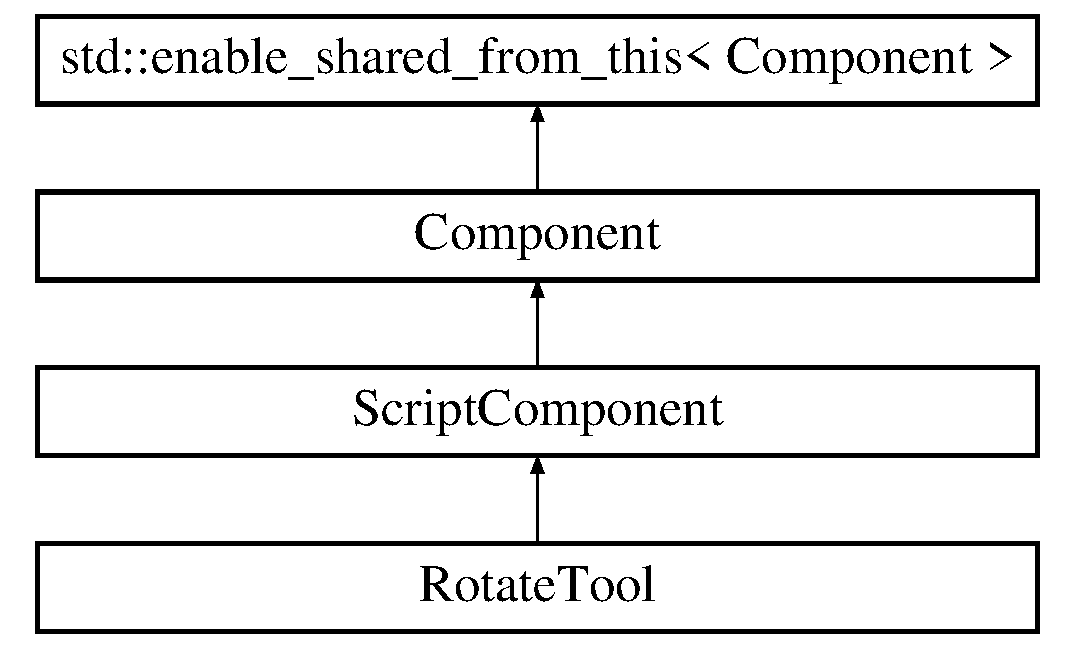
\includegraphics[height=4.000000cm]{class_rotate_tool}
\end{center}
\end{figure}
\subsection*{Public Member Functions}
\begin{DoxyCompactItemize}
\item 
virtual void \hyperlink{class_rotate_tool_af476de7866d44808efd35fe431710049}{awake} () override
\item 
virtual void \hyperlink{class_rotate_tool_a59f02b0a16d0fa6c48a8cf6d2e1fcd70}{tick} (float delta\+Seconds) override
\end{DoxyCompactItemize}
\subsection*{Public Attributes}
\begin{DoxyCompactItemize}
\item 
\hypertarget{class_rotate_tool_a475eb6b578e6fd75dc3be68e70198f1e}{}weak\+\_\+ptr$<$ \hyperlink{class_rotate_handle}{Rotate\+Handle} $>$ {\bfseries x}\label{class_rotate_tool_a475eb6b578e6fd75dc3be68e70198f1e}

\item 
\hypertarget{class_rotate_tool_a36dfc4f3d203b4039b31241a4ad7d0ef}{}weak\+\_\+ptr$<$ \hyperlink{class_rotate_handle}{Rotate\+Handle} $>$ {\bfseries y}\label{class_rotate_tool_a36dfc4f3d203b4039b31241a4ad7d0ef}

\item 
\hypertarget{class_rotate_tool_a3e3b6ffbfb8847fef9032da108a016af}{}weak\+\_\+ptr$<$ \hyperlink{class_rotate_handle}{Rotate\+Handle} $>$ {\bfseries z}\label{class_rotate_tool_a3e3b6ffbfb8847fef9032da108a016af}

\end{DoxyCompactItemize}
\subsection*{Additional Inherited Members}


\subsection{Member Function Documentation}
\hypertarget{class_rotate_tool_af476de7866d44808efd35fe431710049}{}\index{Rotate\+Tool@{Rotate\+Tool}!awake@{awake}}
\index{awake@{awake}!Rotate\+Tool@{Rotate\+Tool}}
\subsubsection[{awake() override}]{\setlength{\rightskip}{0pt plus 5cm}void Rotate\+Tool\+::awake (
\begin{DoxyParamCaption}
{}
\end{DoxyParamCaption}
)\hspace{0.3cm}{\ttfamily [override]}, {\ttfamily [virtual]}}\label{class_rotate_tool_af476de7866d44808efd35fe431710049}
\hyperlink{class_component}{Component} awake override 

Reimplemented from \hyperlink{class_script_component_a4667b8a3712e18b25cd6f49f12c5677d}{Script\+Component}.

\hypertarget{class_rotate_tool_a59f02b0a16d0fa6c48a8cf6d2e1fcd70}{}\index{Rotate\+Tool@{Rotate\+Tool}!tick@{tick}}
\index{tick@{tick}!Rotate\+Tool@{Rotate\+Tool}}
\subsubsection[{tick(float delta\+Seconds) override}]{\setlength{\rightskip}{0pt plus 5cm}void Rotate\+Tool\+::tick (
\begin{DoxyParamCaption}
\item[{float}]{delta\+Secods}
\end{DoxyParamCaption}
)\hspace{0.3cm}{\ttfamily [override]}, {\ttfamily [virtual]}}\label{class_rotate_tool_a59f02b0a16d0fa6c48a8cf6d2e1fcd70}
\hyperlink{class_component}{Component} tick override 
\begin{DoxyParams}[1]{Parameters}
\mbox{\tt in}  & {\em delta\+Seconds} & last frame durations \\
\hline
\end{DoxyParams}


Reimplemented from \hyperlink{class_script_component_aa765fa62a343a8d83eb168d369b93a51}{Script\+Component}.



The documentation for this class was generated from the following files\+:\begin{DoxyCompactItemize}
\item 
/\+Users/guilherme\+\_\+cunha/\+Dev/\+G\+I\+T\+H\+U\+B/\+G\+U\+Inity/\+Source/Rotate\+Tool.\+hpp\item 
/\+Users/guilherme\+\_\+cunha/\+Dev/\+G\+I\+T\+H\+U\+B/\+G\+U\+Inity/\+Source/Rotate\+Tool.\+cpp\end{DoxyCompactItemize}

\hypertarget{class_scale_handle}{}\section{Scale\+Handle Class Reference}
\label{class_scale_handle}\index{Scale\+Handle@{Scale\+Handle}}
Inheritance diagram for Scale\+Handle\+:\begin{figure}[H]
\begin{center}
\leavevmode
\includegraphics[height=4.000000cm]{class_scale_handle}
\end{center}
\end{figure}
\subsection*{Public Member Functions}
\begin{DoxyCompactItemize}
\item 
\hypertarget{class_scale_handle_a945c152809d742987665716a5421264e}{}void {\bfseries set\+Axis} (Transform\+Axis axis)\label{class_scale_handle_a945c152809d742987665716a5421264e}

\item 
virtual void \hyperlink{class_scale_handle_a524669abeef7f0f13edf8e3fd041d44d}{tick} (float delta\+Seconds) override
\end{DoxyCompactItemize}
\subsection*{Public Attributes}
\begin{DoxyCompactItemize}
\item 
\hypertarget{class_scale_handle_af601f274be1e551cf3788cd5868fe3c4}{}Transform\+Axis {\bfseries axis}\label{class_scale_handle_af601f274be1e551cf3788cd5868fe3c4}

\end{DoxyCompactItemize}
\subsection*{Additional Inherited Members}


\subsection{Member Function Documentation}
\hypertarget{class_scale_handle_a524669abeef7f0f13edf8e3fd041d44d}{}\index{Scale\+Handle@{Scale\+Handle}!tick@{tick}}
\index{tick@{tick}!Scale\+Handle@{Scale\+Handle}}
\subsubsection[{tick(float delta\+Seconds) override}]{\setlength{\rightskip}{0pt plus 5cm}void Scale\+Handle\+::tick (
\begin{DoxyParamCaption}
\item[{float}]{delta\+Secods}
\end{DoxyParamCaption}
)\hspace{0.3cm}{\ttfamily [override]}, {\ttfamily [virtual]}}\label{class_scale_handle_a524669abeef7f0f13edf8e3fd041d44d}
\hyperlink{class_component}{Component} tick override 
\begin{DoxyParams}[1]{Parameters}
\mbox{\tt in}  & {\em delta\+Seconds} & last frame durations \\
\hline
\end{DoxyParams}


Reimplemented from \hyperlink{class_script_component_aa765fa62a343a8d83eb168d369b93a51}{Script\+Component}.



The documentation for this class was generated from the following files\+:\begin{DoxyCompactItemize}
\item 
/\+Users/guilherme\+\_\+cunha/\+Dev/\+G\+I\+T\+H\+U\+B/\+G\+U\+Inity/\+Source/Scale\+Handle.\+hpp\item 
/\+Users/guilherme\+\_\+cunha/\+Dev/\+G\+I\+T\+H\+U\+B/\+G\+U\+Inity/\+Source/Scale\+Handle.\+cpp\end{DoxyCompactItemize}

\hypertarget{class_scale_tool}{}\section{Scale\+Tool Class Reference}
\label{class_scale_tool}\index{Scale\+Tool@{Scale\+Tool}}
Inheritance diagram for Scale\+Tool\+:\begin{figure}[H]
\begin{center}
\leavevmode
\includegraphics[height=4.000000cm]{class_scale_tool}
\end{center}
\end{figure}
\subsection*{Public Member Functions}
\begin{DoxyCompactItemize}
\item 
virtual void \hyperlink{class_scale_tool_abd0df3bb4452336ac89b914968b91f39}{awake} () override
\item 
virtual void \hyperlink{class_scale_tool_a7ffc744426c942638ff24331de593496}{tick} (float delta\+Seconds) override
\end{DoxyCompactItemize}
\subsection*{Public Attributes}
\begin{DoxyCompactItemize}
\item 
\hypertarget{class_scale_tool_acbb72413a93ac68025de2178fbba5c04}{}weak\+\_\+ptr$<$ \hyperlink{class_scale_handle}{Scale\+Handle} $>$ {\bfseries forward}\label{class_scale_tool_acbb72413a93ac68025de2178fbba5c04}

\item 
\hypertarget{class_scale_tool_a7c4ec3709e2e7d7788cb5f53aba93cd1}{}weak\+\_\+ptr$<$ \hyperlink{class_scale_handle}{Scale\+Handle} $>$ {\bfseries up}\label{class_scale_tool_a7c4ec3709e2e7d7788cb5f53aba93cd1}

\item 
\hypertarget{class_scale_tool_a9af1ccb894e45369aec42c5b34d8bd29}{}weak\+\_\+ptr$<$ \hyperlink{class_scale_handle}{Scale\+Handle} $>$ {\bfseries right}\label{class_scale_tool_a9af1ccb894e45369aec42c5b34d8bd29}

\end{DoxyCompactItemize}
\subsection*{Additional Inherited Members}


\subsection{Member Function Documentation}
\hypertarget{class_scale_tool_abd0df3bb4452336ac89b914968b91f39}{}\index{Scale\+Tool@{Scale\+Tool}!awake@{awake}}
\index{awake@{awake}!Scale\+Tool@{Scale\+Tool}}
\subsubsection[{awake() override}]{\setlength{\rightskip}{0pt plus 5cm}void Scale\+Tool\+::awake (
\begin{DoxyParamCaption}
{}
\end{DoxyParamCaption}
)\hspace{0.3cm}{\ttfamily [override]}, {\ttfamily [virtual]}}\label{class_scale_tool_abd0df3bb4452336ac89b914968b91f39}
\hyperlink{class_component}{Component} awake override 

Reimplemented from \hyperlink{class_script_component_a4667b8a3712e18b25cd6f49f12c5677d}{Script\+Component}.

\hypertarget{class_scale_tool_a7ffc744426c942638ff24331de593496}{}\index{Scale\+Tool@{Scale\+Tool}!tick@{tick}}
\index{tick@{tick}!Scale\+Tool@{Scale\+Tool}}
\subsubsection[{tick(float delta\+Seconds) override}]{\setlength{\rightskip}{0pt plus 5cm}void Scale\+Tool\+::tick (
\begin{DoxyParamCaption}
\item[{float}]{delta\+Secods}
\end{DoxyParamCaption}
)\hspace{0.3cm}{\ttfamily [override]}, {\ttfamily [virtual]}}\label{class_scale_tool_a7ffc744426c942638ff24331de593496}
\hyperlink{class_component}{Component} tick override 
\begin{DoxyParams}[1]{Parameters}
\mbox{\tt in}  & {\em delta\+Seconds} & last frame durations \\
\hline
\end{DoxyParams}


Reimplemented from \hyperlink{class_script_component_aa765fa62a343a8d83eb168d369b93a51}{Script\+Component}.



The documentation for this class was generated from the following files\+:\begin{DoxyCompactItemize}
\item 
/\+Users/guilherme\+\_\+cunha/\+Dev/\+G\+I\+T\+H\+U\+B/\+G\+U\+Inity/\+Source/Scale\+Tool.\+hpp\item 
/\+Users/guilherme\+\_\+cunha/\+Dev/\+G\+I\+T\+H\+U\+B/\+G\+U\+Inity/\+Source/Scale\+Tool.\+cpp\end{DoxyCompactItemize}

\hypertarget{class_script_component}{}\section{Script\+Component Class Reference}
\label{class_script_component}\index{Script\+Component@{Script\+Component}}


{\ttfamily \#include $<$Script\+Component.\+hpp$>$}

Inheritance diagram for Script\+Component\+:\begin{figure}[H]
\begin{center}
\leavevmode
\includegraphics[height=12.000000cm]{class_script_component}
\end{center}
\end{figure}
\subsection*{Public Member Functions}
\begin{DoxyCompactItemize}
\item 
\hyperlink{class_script_component_a918a8a3ffb5ee72ead98eb693c343620}{Script\+Component} ()
\item 
virtual \hyperlink{class_script_component_a6c266c364bf21d0dddb6d7639500a077}{$\sim$\+Script\+Component} ()
\item 
virtual void \hyperlink{class_script_component_a6fb8a859ed628b7b97801a2b3fb4f8ea}{init} ()
\item 
virtual void \hyperlink{class_script_component_a3e7c2770a1ee8bcc1fd8d39fdb65cc44}{destroy} ()
\item 
virtual void \hyperlink{class_script_component_a4667b8a3712e18b25cd6f49f12c5677d}{awake} () override
\item 
virtual void \hyperlink{class_script_component_aa765fa62a343a8d83eb168d369b93a51}{tick} (float delta\+Secods) override
\item 
virtual void \hyperlink{class_script_component_a9f84fa4e6c97f6b61926164c487fd6af}{on\+Collision} (\hyperlink{class_actor}{Actor} $\ast$actor)
\item 
virtual void \hyperlink{class_script_component_a4632d59065aa53982b6b154d3bc60502}{on\+Trigger} (\hyperlink{class_actor}{Actor} $\ast$actor)
\item 
virtual shared\+\_\+ptr$<$ \hyperlink{class_component}{Component} $>$ \hyperlink{class_script_component_adebdf5187e8f41f68f445ff7555d5036}{clone} () override
\item 
virtual shared\+\_\+ptr$<$ \hyperlink{class_component_description}{Component\+Description} $>$ \hyperlink{group__serialization__functions_ga109d36ec69582f38228ec003039c653a}{get\+Component\+Description} () override
\item 
virtual void \hyperlink{group__serialization__functions_ga0fc188eda2331400a0bc2b5ecfd8221e}{deserialize} (shared\+\_\+ptr$<$ \hyperlink{class_component_description}{Component\+Description} $>$ desc) override
\end{DoxyCompactItemize}
\subsection*{Additional Inherited Members}


\subsection{Detailed Description}
\hyperlink{class_script_component}{Script\+Component} is a \hyperlink{class_component}{Component} that allows for Custom Behaviour. For example the controller of a space ship, a manager or anything that needs its own specific rules. 

\subsection{Constructor \& Destructor Documentation}
\hypertarget{class_script_component_a918a8a3ffb5ee72ead98eb693c343620}{}\index{Script\+Component@{Script\+Component}!Script\+Component@{Script\+Component}}
\index{Script\+Component@{Script\+Component}!Script\+Component@{Script\+Component}}
\subsubsection[{Script\+Component()}]{\setlength{\rightskip}{0pt plus 5cm}Script\+Component\+::\+Script\+Component (
\begin{DoxyParamCaption}
{}
\end{DoxyParamCaption}
)}\label{class_script_component_a918a8a3ffb5ee72ead98eb693c343620}
Default Constructor \hypertarget{class_script_component_a6c266c364bf21d0dddb6d7639500a077}{}\index{Script\+Component@{Script\+Component}!````~Script\+Component@{$\sim$\+Script\+Component}}
\index{````~Script\+Component@{$\sim$\+Script\+Component}!Script\+Component@{Script\+Component}}
\subsubsection[{$\sim$\+Script\+Component()}]{\setlength{\rightskip}{0pt plus 5cm}Script\+Component\+::$\sim$\+Script\+Component (
\begin{DoxyParamCaption}
{}
\end{DoxyParamCaption}
)\hspace{0.3cm}{\ttfamily [virtual]}}\label{class_script_component_a6c266c364bf21d0dddb6d7639500a077}
Default Destructor 

\subsection{Member Function Documentation}
\hypertarget{class_script_component_a4667b8a3712e18b25cd6f49f12c5677d}{}\index{Script\+Component@{Script\+Component}!awake@{awake}}
\index{awake@{awake}!Script\+Component@{Script\+Component}}
\subsubsection[{awake() override}]{\setlength{\rightskip}{0pt plus 5cm}virtual void Script\+Component\+::awake (
\begin{DoxyParamCaption}
{}
\end{DoxyParamCaption}
)\hspace{0.3cm}{\ttfamily [inline]}, {\ttfamily [override]}, {\ttfamily [virtual]}}\label{class_script_component_a4667b8a3712e18b25cd6f49f12c5677d}
\hyperlink{class_component}{Component} awake override 

Reimplemented from \hyperlink{class_component_ae413974ecdbc8f65c6ff707b84278b0e}{Component}.



Reimplemented in \hyperlink{class_scale_tool_abd0df3bb4452336ac89b914968b91f39}{Scale\+Tool}, \hyperlink{class_player_script_acb623eb7cdcfc49b7848bf7d60809cb7}{Player\+Script}, \hyperlink{class_move_tool_ac53066bdb36f2e01234fa58a20cc1f0d}{Move\+Tool}, \hyperlink{class_rotate_handle_a93caa7dd2992d5dc3fcef9cbc4278bed}{Rotate\+Handle}, \hyperlink{class_rotate_tool_af476de7866d44808efd35fe431710049}{Rotate\+Tool}, and \hyperlink{class_increase_collider_script_a2a3291f10ec9cd908a0c45992847d7fe}{Increase\+Collider\+Script}.

\hypertarget{class_script_component_adebdf5187e8f41f68f445ff7555d5036}{}\index{Script\+Component@{Script\+Component}!clone@{clone}}
\index{clone@{clone}!Script\+Component@{Script\+Component}}
\subsubsection[{clone() override}]{\setlength{\rightskip}{0pt plus 5cm}shared\+\_\+ptr$<$ {\bf Component} $>$ Script\+Component\+::clone (
\begin{DoxyParamCaption}
{}
\end{DoxyParamCaption}
)\hspace{0.3cm}{\ttfamily [override]}, {\ttfamily [virtual]}}\label{class_script_component_adebdf5187e8f41f68f445ff7555d5036}
Clones current component (Prototype Design Pattern) \begin{DoxyReturn}{Returns}
shared\+\_\+ptr to cloned \hyperlink{class_script_component}{Script\+Component} \hyperlink{class_component}{Component} 
\end{DoxyReturn}


Implements \hyperlink{class_component_a74c984bd819bbef16fd4f306a90d34fe}{Component}.



Reimplemented in \hyperlink{class_player_script_a75a83f06a2acb93ce1a629dcf2dabf5c}{Player\+Script}.

\hypertarget{class_script_component_a3e7c2770a1ee8bcc1fd8d39fdb65cc44}{}\index{Script\+Component@{Script\+Component}!destroy@{destroy}}
\index{destroy@{destroy}!Script\+Component@{Script\+Component}}
\subsubsection[{destroy()}]{\setlength{\rightskip}{0pt plus 5cm}virtual void Script\+Component\+::destroy (
\begin{DoxyParamCaption}
{}
\end{DoxyParamCaption}
)\hspace{0.3cm}{\ttfamily [inline]}, {\ttfamily [virtual]}}\label{class_script_component_a3e7c2770a1ee8bcc1fd8d39fdb65cc44}
\hyperlink{class_component}{Component} destroy override 

Reimplemented from \hyperlink{class_component_a77b8fff56ddce5dd0b4a9dabb0b5202b}{Component}.

\hypertarget{class_script_component_a6fb8a859ed628b7b97801a2b3fb4f8ea}{}\index{Script\+Component@{Script\+Component}!init@{init}}
\index{init@{init}!Script\+Component@{Script\+Component}}
\subsubsection[{init()}]{\setlength{\rightskip}{0pt plus 5cm}virtual void Script\+Component\+::init (
\begin{DoxyParamCaption}
{}
\end{DoxyParamCaption}
)\hspace{0.3cm}{\ttfamily [inline]}, {\ttfamily [virtual]}}\label{class_script_component_a6fb8a859ed628b7b97801a2b3fb4f8ea}
\hyperlink{class_component}{Component} init override 

Reimplemented from \hyperlink{class_component_a162f8cdc070537a71f2ad0b5e763b86f}{Component}.



Reimplemented in \hyperlink{class_editor_camera_control_af672d52ea342e6762f9f104898959181}{Editor\+Camera\+Control}.

\hypertarget{class_script_component_a9f84fa4e6c97f6b61926164c487fd6af}{}\index{Script\+Component@{Script\+Component}!on\+Collision@{on\+Collision}}
\index{on\+Collision@{on\+Collision}!Script\+Component@{Script\+Component}}
\subsubsection[{on\+Collision(\+Actor $\ast$actor)}]{\setlength{\rightskip}{0pt plus 5cm}virtual void Script\+Component\+::on\+Collision (
\begin{DoxyParamCaption}
\item[{{\bf Actor} $\ast$}]{actor}
\end{DoxyParamCaption}
)\hspace{0.3cm}{\ttfamily [inline]}, {\ttfamily [virtual]}}\label{class_script_component_a9f84fa4e6c97f6b61926164c487fd6af}
Callback function called when a collision occurs 

Reimplemented in \hyperlink{class_player_script_aa57ebbefa2e5be812b9a0272ae654258}{Player\+Script}.

\hypertarget{class_script_component_a4632d59065aa53982b6b154d3bc60502}{}\index{Script\+Component@{Script\+Component}!on\+Trigger@{on\+Trigger}}
\index{on\+Trigger@{on\+Trigger}!Script\+Component@{Script\+Component}}
\subsubsection[{on\+Trigger(\+Actor $\ast$actor)}]{\setlength{\rightskip}{0pt plus 5cm}virtual void Script\+Component\+::on\+Trigger (
\begin{DoxyParamCaption}
\item[{{\bf Actor} $\ast$}]{actor}
\end{DoxyParamCaption}
)\hspace{0.3cm}{\ttfamily [inline]}, {\ttfamily [virtual]}}\label{class_script_component_a4632d59065aa53982b6b154d3bc60502}
Callback function called when a trigger collision occurs 

Reimplemented in \hyperlink{class_player_script_ad5476bdc3f1b168047def498cd62844f}{Player\+Script}.

\hypertarget{class_script_component_aa765fa62a343a8d83eb168d369b93a51}{}\index{Script\+Component@{Script\+Component}!tick@{tick}}
\index{tick@{tick}!Script\+Component@{Script\+Component}}
\subsubsection[{tick(float delta\+Secods) override}]{\setlength{\rightskip}{0pt plus 5cm}virtual void Script\+Component\+::tick (
\begin{DoxyParamCaption}
\item[{float}]{delta\+Secods}
\end{DoxyParamCaption}
)\hspace{0.3cm}{\ttfamily [inline]}, {\ttfamily [override]}, {\ttfamily [virtual]}}\label{class_script_component_aa765fa62a343a8d83eb168d369b93a51}
\hyperlink{class_component}{Component} tick override 
\begin{DoxyParams}[1]{Parameters}
\mbox{\tt in}  & {\em delta\+Seconds} & last frame durations \\
\hline
\end{DoxyParams}


Reimplemented from \hyperlink{class_component_a72d67b02e6733c1a6fb73cbaaf8ebff4}{Component}.



Reimplemented in \hyperlink{class_scale_handle_a524669abeef7f0f13edf8e3fd041d44d}{Scale\+Handle}, \hyperlink{class_scale_tool_a7ffc744426c942638ff24331de593496}{Scale\+Tool}, \hyperlink{class_player_script_a5cd8853a54348831521f0455df5b508c}{Player\+Script}, \hyperlink{class_move_handle_a39cb33cbbf841fee4d07c8a8cc380128}{Move\+Handle}, \hyperlink{class_rotate_over_time_a57f0412df19fefd4ab4dd11839c483e1}{Rotate\+Over\+Time}, \hyperlink{class_add_force_script_a8ad91eeecbfae666a28c44345d59251d}{Add\+Force\+Script}, \hyperlink{class_move_tool_ad38e6fcb03e6d7b2f0ef241ec0eb5271}{Move\+Tool}, \hyperlink{class_rotate_handle_a58b0a9ebbcd28378aed805628107eef4}{Rotate\+Handle}, \hyperlink{class_editor_camera_control_a829966c94f5f99911a20534692dcc78f}{Editor\+Camera\+Control}, \hyperlink{class_rotate_tool_a59f02b0a16d0fa6c48a8cf6d2e1fcd70}{Rotate\+Tool}, and \hyperlink{class_increase_collider_script_a7be665f5544316bfd2ad39c32e66b11f}{Increase\+Collider\+Script}.



The documentation for this class was generated from the following files\+:\begin{DoxyCompactItemize}
\item 
/\+Users/guilherme\+\_\+cunha/\+Dev/\+G\+I\+T\+H\+U\+B/\+G\+U\+Inity/\+Source/Script\+Component.\+hpp\item 
/\+Users/guilherme\+\_\+cunha/\+Dev/\+G\+I\+T\+H\+U\+B/\+G\+U\+Inity/\+Source/Script\+Component.\+cpp\end{DoxyCompactItemize}

\hypertarget{class_shader}{}\section{Shader Class Reference}
\label{class_shader}\index{Shader@{Shader}}
Inheritance diagram for Shader\+:\begin{figure}[H]
\begin{center}
\leavevmode
\includegraphics[height=2.000000cm]{class_shader}
\end{center}
\end{figure}
\subsection*{Public Member Functions}
\begin{DoxyCompactItemize}
\item 
\hypertarget{class_shader_a71fc7c649e38febf8bb7b595855fd631}{}{\bfseries Shader} (string vertex\+\_\+file\+\_\+path, string fragment\+\_\+file\+\_\+path)\label{class_shader_a71fc7c649e38febf8bb7b595855fd631}

\item 
\hypertarget{class_shader_a44ff58703bdc37626f73051ad06650fd}{}void {\bfseries Load\+Shaders} ()\label{class_shader_a44ff58703bdc37626f73051ad06650fd}

\item 
\hypertarget{class_shader_a06e03a6849c1729778b71ffaf0f4f743}{}void {\bfseries check\+Line} (const string \&Line)\label{class_shader_a06e03a6849c1729778b71ffaf0f4f743}

\item 
\hypertarget{class_shader_a46bff156441ba67d54d7487317deb71b}{}void {\bfseries create\+Uniform\+Location} ()\label{class_shader_a46bff156441ba67d54d7487317deb71b}

\end{DoxyCompactItemize}
\subsection*{Public Attributes}
\begin{DoxyCompactItemize}
\item 
\hypertarget{class_shader_af5c648f5ea74908dd3ad9aae91d0e61a}{}string {\bfseries vs\+Filename}\label{class_shader_af5c648f5ea74908dd3ad9aae91d0e61a}

\item 
\hypertarget{class_shader_a0eb039600af333cc4c4e424dbc5c2068}{}string {\bfseries fs\+Filename}\label{class_shader_a0eb039600af333cc4c4e424dbc5c2068}

\item 
\hypertarget{class_shader_ac693a3dd588572cc848e109f15418268}{}map$<$ string, Shader\+Param\+Type $>$ {\bfseries params}\label{class_shader_ac693a3dd588572cc848e109f15418268}

\item 
\hypertarget{class_shader_aff452b0d16cca218ca27fbb46d5139a6}{}map$<$ string, G\+Luint $>$ {\bfseries param\+I\+D}\label{class_shader_aff452b0d16cca218ca27fbb46d5139a6}

\item 
\hypertarget{class_shader_afce507f5013e82f7a62b47bbfb2fb048}{}G\+Luint {\bfseries program\+I\+D}\label{class_shader_afce507f5013e82f7a62b47bbfb2fb048}

\end{DoxyCompactItemize}


The documentation for this class was generated from the following files\+:\begin{DoxyCompactItemize}
\item 
/\+Users/guilherme\+\_\+cunha/\+Dev/\+G\+I\+T\+H\+U\+B/\+G\+U\+Inity/\+Source/Shader.\+hpp\item 
/\+Users/guilherme\+\_\+cunha/\+Dev/\+G\+I\+T\+H\+U\+B/\+G\+U\+Inity/\+Source/Shader.\+cpp\end{DoxyCompactItemize}

\hypertarget{class_skinned_mesh}{}\section{Skinned\+Mesh Class Reference}
\label{class_skinned_mesh}\index{Skinned\+Mesh@{Skinned\+Mesh}}
Inheritance diagram for Skinned\+Mesh\+:\begin{figure}[H]
\begin{center}
\leavevmode
\includegraphics[height=3.000000cm]{class_skinned_mesh}
\end{center}
\end{figure}
\subsection*{Public Member Functions}
\begin{DoxyCompactItemize}
\item 
\hypertarget{class_skinned_mesh_a612bb08a70f98fc4be45615592dadf5c}{}void {\bfseries set\+N\+Bones} (int n\+Bones)\label{class_skinned_mesh_a612bb08a70f98fc4be45615592dadf5c}

\item 
\hypertarget{class_skinned_mesh_ab8f404e4843d76e02387517ec7cc3cee}{}int {\bfseries get\+N\+Bones} ()\label{class_skinned_mesh_ab8f404e4843d76e02387517ec7cc3cee}

\item 
void \hyperlink{class_skinned_mesh_a185a679f88fdf60177196b3f1f591e4f}{set\+Vertices\+Weight} (vector$<$ vector$<$ float $>$$>$ weights)
\item 
\hypertarget{class_skinned_mesh_a70912234b58d31ab8aee540d3fb288a8}{}void {\bfseries set\+Initial\+Position} (vector$<$ glm\+::mat4 $>$ initial\+Pos)\label{class_skinned_mesh_a70912234b58d31ab8aee540d3fb288a8}

\end{DoxyCompactItemize}
\subsection*{Additional Inherited Members}


\subsection{Member Function Documentation}
\hypertarget{class_skinned_mesh_a185a679f88fdf60177196b3f1f591e4f}{}\index{Skinned\+Mesh@{Skinned\+Mesh}!set\+Vertices\+Weight@{set\+Vertices\+Weight}}
\index{set\+Vertices\+Weight@{set\+Vertices\+Weight}!Skinned\+Mesh@{Skinned\+Mesh}}
\subsubsection[{set\+Vertices\+Weight(vector$<$ vector$<$ float $>$$>$ weights)}]{\setlength{\rightskip}{0pt plus 5cm}void Skinned\+Mesh\+::set\+Vertices\+Weight (
\begin{DoxyParamCaption}
\item[{vector$<$ vector$<$ float $>$$>$}]{weights}
\end{DoxyParamCaption}
)}\label{class_skinned_mesh_a185a679f88fdf60177196b3f1f591e4f}
Adds a new vertex to the mesh 

The documentation for this class was generated from the following files\+:\begin{DoxyCompactItemize}
\item 
/\+Users/guilherme\+\_\+cunha/\+Dev/\+G\+I\+T\+H\+U\+B/\+G\+U\+Inity/\+Source/Skinned\+Mesh.\+hpp\item 
/\+Users/guilherme\+\_\+cunha/\+Dev/\+G\+I\+T\+H\+U\+B/\+G\+U\+Inity/\+Source/Skinned\+Mesh.\+cpp\end{DoxyCompactItemize}

\hypertarget{class_sound}{}\section{Sound Class Reference}
\label{class_sound}\index{Sound@{Sound}}
Inheritance diagram for Sound\+:\begin{figure}[H]
\begin{center}
\leavevmode
\includegraphics[height=2.000000cm]{class_sound}
\end{center}
\end{figure}
\subsection*{Public Member Functions}
\begin{DoxyCompactItemize}
\item 
\hypertarget{class_sound_aa621785a9569bcd0724a7498c287b10d}{}{\bfseries Sound} (string filename)\label{class_sound_aa621785a9569bcd0724a7498c287b10d}

\end{DoxyCompactItemize}
\subsection*{Public Attributes}
\begin{DoxyCompactItemize}
\item 
\hypertarget{class_sound_acd62674bebee2a659ba2d9bc0e84114f}{}F\+M\+O\+D\+::\+Sound $\ast$ {\bfseries sound\+Handle}\label{class_sound_acd62674bebee2a659ba2d9bc0e84114f}

\end{DoxyCompactItemize}


The documentation for this class was generated from the following files\+:\begin{DoxyCompactItemize}
\item 
/\+Users/guilherme\+\_\+cunha/\+Dev/\+G\+I\+T\+H\+U\+B/\+G\+U\+Inity/\+Source/Sound.\+hpp\item 
/\+Users/guilherme\+\_\+cunha/\+Dev/\+G\+I\+T\+H\+U\+B/\+G\+U\+Inity/\+Source/Sound.\+cpp\end{DoxyCompactItemize}

\hypertarget{class_sound_system}{}\section{Sound\+System Class Reference}
\label{class_sound_system}\index{Sound\+System@{Sound\+System}}
\subsection*{Public Member Functions}
\begin{DoxyCompactItemize}
\item 
\hypertarget{class_sound_system_adcb1d5df10d30863c668ac51102d680f}{}int {\bfseries init} ()\label{class_sound_system_adcb1d5df10d30863c668ac51102d680f}

\item 
\hypertarget{class_sound_system_a9c9f6c3017fba3fb02c226ea18940e7e}{}void {\bfseries shutdown} ()\label{class_sound_system_a9c9f6c3017fba3fb02c226ea18940e7e}

\item 
\hypertarget{class_sound_system_a67255f0007de8a4257bd214be5aecf9c}{}void {\bfseries play\+Sound} (shared\+\_\+ptr$<$ \hyperlink{class_sound}{Sound} $>$ sound)\label{class_sound_system_a67255f0007de8a4257bd214be5aecf9c}

\item 
\hypertarget{class_sound_system_a8ceb6af1ebfa69a61dfaed29f28a9b0c}{}F\+M\+O\+D\+\_\+\+R\+E\+S\+U\+L\+T {\bfseries create\+Sound} (string filename, int mode, F\+M\+O\+D\+\_\+\+C\+R\+E\+A\+T\+E\+S\+O\+U\+N\+D\+E\+X\+I\+N\+F\+O $\ast$ex\+Info, F\+M\+O\+D\+::\+Sound $\ast$$\ast$sound)\label{class_sound_system_a8ceb6af1ebfa69a61dfaed29f28a9b0c}

\end{DoxyCompactItemize}
\subsection*{Static Public Member Functions}
\begin{DoxyCompactItemize}
\item 
\hypertarget{class_sound_system_a7f6fe1a45ed73411b42ee0c18cc184d7}{}static \hyperlink{class_sound_system}{Sound\+System} $\ast$ {\bfseries get\+Instance} ()\label{class_sound_system_a7f6fe1a45ed73411b42ee0c18cc184d7}

\end{DoxyCompactItemize}
\subsection*{Public Attributes}
\begin{DoxyCompactItemize}
\item 
\hypertarget{class_sound_system_ada6f06657608c32304d30f4ef8825256}{}F\+M\+O\+D\+::\+System $\ast$ {\bfseries system}\label{class_sound_system_ada6f06657608c32304d30f4ef8825256}

\item 
\hypertarget{class_sound_system_a7ce2104c8728b305f84c120bc59058d6}{}F\+M\+O\+D\+::\+Channel $\ast$ {\bfseries channel}\label{class_sound_system_a7ce2104c8728b305f84c120bc59058d6}

\end{DoxyCompactItemize}


The documentation for this class was generated from the following files\+:\begin{DoxyCompactItemize}
\item 
/\+Users/guilherme\+\_\+cunha/\+Dev/\+G\+I\+T\+H\+U\+B/\+G\+U\+Inity/\+Source/Sound\+System.\+hpp\item 
/\+Users/guilherme\+\_\+cunha/\+Dev/\+G\+I\+T\+H\+U\+B/\+G\+U\+Inity/\+Source/Sound\+System.\+cpp\end{DoxyCompactItemize}

\hypertarget{class_sphere_collider}{}\section{Sphere\+Collider Class Reference}
\label{class_sphere_collider}\index{Sphere\+Collider@{Sphere\+Collider}}


{\ttfamily \#include $<$Sphere\+Collider.\+hpp$>$}

Inheritance diagram for Sphere\+Collider\+:\begin{figure}[H]
\begin{center}
\leavevmode
\includegraphics[height=4.000000cm]{class_sphere_collider}
\end{center}
\end{figure}
\subsection*{Public Member Functions}
\begin{DoxyCompactItemize}
\item 
\hyperlink{class_sphere_collider_af46ca28e45d8efa559f097aadfb9bc44}{Sphere\+Collider} ()
\item 
\hyperlink{class_sphere_collider_a9e4b771c5e43efbbc75aa8359748e514}{Sphere\+Collider} (float radius, Px\+Vec3 \hyperlink{class_collider_a42b57aa35ab665daf89ae844e479c560}{center})
\item 
virtual \hyperlink{class_sphere_collider_ac3f355cae4d6cbd988bf7b4ea74b5472}{$\sim$\+Sphere\+Collider} ()
\item 
float \hyperlink{class_sphere_collider_af9a9507ea31d7ce40dbf2bf3399a731b}{get\+Radius} ()
\item 
void \hyperlink{class_sphere_collider_ae8fb3c78c7cda1b89dbdb569961fef63}{set\+Radius} (float new\+Radius)
\item 
virtual void \hyperlink{class_sphere_collider_aa51773fa54349bec5730b3ae528c4179}{init} ()
\item 
virtual shared\+\_\+ptr$<$ \hyperlink{class_component}{Component} $>$ \hyperlink{class_sphere_collider_a68cd4eaf4ee2b13ac48efc38a760ff36}{clone} () override
\item 
virtual shared\+\_\+ptr$<$ \hyperlink{class_component_description}{Component\+Description} $>$ \hyperlink{group__serialization__functions_gac6dec979a6872bf1ca8a78fb2f44c511}{get\+Component\+Description} () override
\item 
virtual void \hyperlink{group__serialization__functions_ga26f4dcd8bdc47e087b7e8f57c7879ca0}{deserialize} (shared\+\_\+ptr$<$ \hyperlink{class_component_description}{Component\+Description} $>$ desc) override
\end{DoxyCompactItemize}
\subsection*{Additional Inherited Members}


\subsection{Detailed Description}
\hyperlink{class_sphere_collider}{Sphere\+Collider} uses a sphere as the volume collider. Can either be real physics simulated or trigger only. 

\subsection{Constructor \& Destructor Documentation}
\hypertarget{class_sphere_collider_af46ca28e45d8efa559f097aadfb9bc44}{}\index{Sphere\+Collider@{Sphere\+Collider}!Sphere\+Collider@{Sphere\+Collider}}
\index{Sphere\+Collider@{Sphere\+Collider}!Sphere\+Collider@{Sphere\+Collider}}
\subsubsection[{Sphere\+Collider()}]{\setlength{\rightskip}{0pt plus 5cm}Sphere\+Collider\+::\+Sphere\+Collider (
\begin{DoxyParamCaption}
{}
\end{DoxyParamCaption}
)}\label{class_sphere_collider_af46ca28e45d8efa559f097aadfb9bc44}
Default Constructor \hypertarget{class_sphere_collider_a9e4b771c5e43efbbc75aa8359748e514}{}\index{Sphere\+Collider@{Sphere\+Collider}!Sphere\+Collider@{Sphere\+Collider}}
\index{Sphere\+Collider@{Sphere\+Collider}!Sphere\+Collider@{Sphere\+Collider}}
\subsubsection[{Sphere\+Collider(float radius, Px\+Vec3 center)}]{\setlength{\rightskip}{0pt plus 5cm}Sphere\+Collider\+::\+Sphere\+Collider (
\begin{DoxyParamCaption}
\item[{float}]{radius, }
\item[{Px\+Vec3}]{center = {\ttfamily PxVec3(0,0,0)}}
\end{DoxyParamCaption}
)}\label{class_sphere_collider_a9e4b771c5e43efbbc75aa8359748e514}
Deserialization Constructor \hypertarget{class_sphere_collider_ac3f355cae4d6cbd988bf7b4ea74b5472}{}\index{Sphere\+Collider@{Sphere\+Collider}!````~Sphere\+Collider@{$\sim$\+Sphere\+Collider}}
\index{````~Sphere\+Collider@{$\sim$\+Sphere\+Collider}!Sphere\+Collider@{Sphere\+Collider}}
\subsubsection[{$\sim$\+Sphere\+Collider()}]{\setlength{\rightskip}{0pt plus 5cm}Sphere\+Collider\+::$\sim$\+Sphere\+Collider (
\begin{DoxyParamCaption}
{}
\end{DoxyParamCaption}
)\hspace{0.3cm}{\ttfamily [virtual]}}\label{class_sphere_collider_ac3f355cae4d6cbd988bf7b4ea74b5472}
Default Destructor 

\subsection{Member Function Documentation}
\hypertarget{class_sphere_collider_a68cd4eaf4ee2b13ac48efc38a760ff36}{}\index{Sphere\+Collider@{Sphere\+Collider}!clone@{clone}}
\index{clone@{clone}!Sphere\+Collider@{Sphere\+Collider}}
\subsubsection[{clone() override}]{\setlength{\rightskip}{0pt plus 5cm}shared\+\_\+ptr$<$ {\bf Component} $>$ Sphere\+Collider\+::clone (
\begin{DoxyParamCaption}
{}
\end{DoxyParamCaption}
)\hspace{0.3cm}{\ttfamily [override]}, {\ttfamily [virtual]}}\label{class_sphere_collider_a68cd4eaf4ee2b13ac48efc38a760ff36}
Clones current component (Prototype Design Pattern) \begin{DoxyReturn}{Returns}
shared\+\_\+ptr to cloned \hyperlink{class_sphere_collider}{Sphere\+Collider} \hyperlink{class_component}{Component} 
\end{DoxyReturn}


Implements \hyperlink{class_collider_a28d0829db9804b27590afc9979e61a1c}{Collider}.

\hypertarget{class_sphere_collider_af9a9507ea31d7ce40dbf2bf3399a731b}{}\index{Sphere\+Collider@{Sphere\+Collider}!get\+Radius@{get\+Radius}}
\index{get\+Radius@{get\+Radius}!Sphere\+Collider@{Sphere\+Collider}}
\subsubsection[{get\+Radius()}]{\setlength{\rightskip}{0pt plus 5cm}float Sphere\+Collider\+::get\+Radius (
\begin{DoxyParamCaption}
{}
\end{DoxyParamCaption}
)}\label{class_sphere_collider_af9a9507ea31d7ce40dbf2bf3399a731b}
radius Getter \begin{DoxyReturn}{Returns}
radius of the sphere 
\end{DoxyReturn}
\hypertarget{class_sphere_collider_aa51773fa54349bec5730b3ae528c4179}{}\index{Sphere\+Collider@{Sphere\+Collider}!init@{init}}
\index{init@{init}!Sphere\+Collider@{Sphere\+Collider}}
\subsubsection[{init()}]{\setlength{\rightskip}{0pt plus 5cm}void Sphere\+Collider\+::init (
\begin{DoxyParamCaption}
{}
\end{DoxyParamCaption}
)\hspace{0.3cm}{\ttfamily [virtual]}}\label{class_sphere_collider_aa51773fa54349bec5730b3ae528c4179}
Init component override. Create a new Sphere Shape in the Phys\+X scene. 

Reimplemented from \hyperlink{class_collider_aed04ad82be15bcba1d3dc6a09f76dae6}{Collider}.

\hypertarget{class_sphere_collider_ae8fb3c78c7cda1b89dbdb569961fef63}{}\index{Sphere\+Collider@{Sphere\+Collider}!set\+Radius@{set\+Radius}}
\index{set\+Radius@{set\+Radius}!Sphere\+Collider@{Sphere\+Collider}}
\subsubsection[{set\+Radius(float new\+Radius)}]{\setlength{\rightskip}{0pt plus 5cm}void Sphere\+Collider\+::set\+Radius (
\begin{DoxyParamCaption}
\item[{float}]{new\+Radius}
\end{DoxyParamCaption}
)}\label{class_sphere_collider_ae8fb3c78c7cda1b89dbdb569961fef63}
radius Setter 
\begin{DoxyParams}[1]{Parameters}
\mbox{\tt in}  & {\em new\+Radius} & the radius of the sphere \\
\hline
\end{DoxyParams}


The documentation for this class was generated from the following files\+:\begin{DoxyCompactItemize}
\item 
/\+Users/guilherme\+\_\+cunha/\+Dev/\+G\+I\+T\+H\+U\+B/\+G\+U\+Inity/\+Source/Sphere\+Collider.\+hpp\item 
/\+Users/guilherme\+\_\+cunha/\+Dev/\+G\+I\+T\+H\+U\+B/\+G\+U\+Inity/\+Source/Sphere\+Collider.\+cpp\end{DoxyCompactItemize}

\hypertarget{class_sphere_collider_description}{}\section{Sphere\+Collider\+Description Class Reference}
\label{class_sphere_collider_description}\index{Sphere\+Collider\+Description@{Sphere\+Collider\+Description}}
Inheritance diagram for Sphere\+Collider\+Description\+:\begin{figure}[H]
\begin{center}
\leavevmode
\includegraphics[height=3.000000cm]{class_sphere_collider_description}
\end{center}
\end{figure}
\subsection*{Public Member Functions}
\begin{DoxyCompactItemize}
\item 
\hypertarget{class_sphere_collider_description_aca0d6e9f7147d60e2db61fb726b6e328}{}{\bfseries Sphere\+Collider\+Description} (float r)\label{class_sphere_collider_description_aca0d6e9f7147d60e2db61fb726b6e328}

\end{DoxyCompactItemize}
\subsection*{Public Attributes}
\begin{DoxyCompactItemize}
\item 
\hypertarget{class_sphere_collider_description_a004e6b84a3e68f74446b33d1fac63f06}{}float {\bfseries radius}\label{class_sphere_collider_description_a004e6b84a3e68f74446b33d1fac63f06}

\end{DoxyCompactItemize}


The documentation for this class was generated from the following file\+:\begin{DoxyCompactItemize}
\item 
/\+Users/guilherme\+\_\+cunha/\+Dev/\+G\+I\+T\+H\+U\+B/\+G\+U\+Inity/\+Source/Serialization\+Structs.\+hpp\end{DoxyCompactItemize}

\hypertarget{class_spline}{}\section{Spline Class Reference}
\label{class_spline}\index{Spline@{Spline}}
\subsection*{Public Member Functions}
\begin{DoxyCompactItemize}
\item 
\hypertarget{class_spline_a362edea61055caf618d97e2c497b906b}{}glm\+::vec3 {\bfseries evaluate3\+D} (float t)\label{class_spline_a362edea61055caf618d97e2c497b906b}

\item 
\hypertarget{class_spline_abc6b72ed5a74f1990efa26bc0058c7f4}{}glm\+::vec2 {\bfseries evaluate2\+D} (float t)\label{class_spline_abc6b72ed5a74f1990efa26bc0058c7f4}

\item 
\hypertarget{class_spline_a478aa5a9a0f6db557f752deef15f2689}{}double {\bfseries evaluate} (float t)\label{class_spline_a478aa5a9a0f6db557f752deef15f2689}

\end{DoxyCompactItemize}


The documentation for this class was generated from the following files\+:\begin{DoxyCompactItemize}
\item 
/\+Users/guilherme\+\_\+cunha/\+Dev/\+G\+I\+T\+H\+U\+B/\+G\+U\+Inity/\+Source/Spline.\+hpp\item 
/\+Users/guilherme\+\_\+cunha/\+Dev/\+G\+I\+T\+H\+U\+B/\+G\+U\+Inity/\+Source/Spline.\+cpp\end{DoxyCompactItemize}

\hypertarget{class_static_counter}{}\section{Static\+Counter$<$ T $>$ Class Template Reference}
\label{class_static_counter}\index{Static\+Counter$<$ T $>$@{Static\+Counter$<$ T $>$}}
\subsection*{Static Public Attributes}
\begin{DoxyCompactItemize}
\item 
\hypertarget{class_static_counter_a6ba3e5bb1cbd9cd9d74c222ae0df2dc4}{}static int {\bfseries n\+Count}\label{class_static_counter_a6ba3e5bb1cbd9cd9d74c222ae0df2dc4}

\end{DoxyCompactItemize}


The documentation for this class was generated from the following file\+:\begin{DoxyCompactItemize}
\item 
/\+Users/guilherme\+\_\+cunha/\+Dev/\+G\+I\+T\+H\+U\+B/\+G\+U\+Inity/\+Source/Static\+Counter.\+hpp\end{DoxyCompactItemize}

\hypertarget{class_subject}{}\section{Subject$<$ T $>$ Class Template Reference}
\label{class_subject}\index{Subject$<$ T $>$@{Subject$<$ T $>$}}
\subsection*{Static Public Member Functions}
\begin{DoxyCompactItemize}
\item 
\hypertarget{class_subject_acf08f1e6c3a24c7f54339b5701eca91c}{}static void {\bfseries add\+Observer} (shared\+\_\+ptr$<$ \hyperlink{class_observer}{Observer} $>$ observer)\label{class_subject_acf08f1e6c3a24c7f54339b5701eca91c}

\item 
\hypertarget{class_subject_ae19850b5b82bd0491eb1574014f567da}{}static void {\bfseries remove\+Observer} (shared\+\_\+ptr$<$ \hyperlink{class_observer}{Observer} $>$ observer)\label{class_subject_ae19850b5b82bd0491eb1574014f567da}

\end{DoxyCompactItemize}
\subsection*{Static Protected Member Functions}
\begin{DoxyCompactItemize}
\item 
\hypertarget{class_subject_ace7d9f4f390b55e8b8d00b48975764b3}{}static void {\bfseries notify} (Component\+Event\+Type type, shared\+\_\+ptr$<$ \hyperlink{class_component}{Component} $>$ component, bool is\+Editor)\label{class_subject_ace7d9f4f390b55e8b8d00b48975764b3}

\item 
\hypertarget{class_subject_aa06d86a66c1aa02f718c8a8cd76ee508}{}static void {\bfseries notify} (Actor\+Event\+Type type, shared\+\_\+ptr$<$ \hyperlink{class_actor}{Actor} $>$ actor, bool is\+Editor)\label{class_subject_aa06d86a66c1aa02f718c8a8cd76ee508}

\end{DoxyCompactItemize}


The documentation for this class was generated from the following file\+:\begin{DoxyCompactItemize}
\item 
/\+Users/guilherme\+\_\+cunha/\+Dev/\+G\+I\+T\+H\+U\+B/\+G\+U\+Inity/\+Source/Subject.\+hpp\end{DoxyCompactItemize}

\hypertarget{class_texture}{}\section{Texture Class Reference}
\label{class_texture}\index{Texture@{Texture}}
Inheritance diagram for Texture\+:\begin{figure}[H]
\begin{center}
\leavevmode
\includegraphics[height=2.000000cm]{class_texture}
\end{center}
\end{figure}
\subsection*{Public Member Functions}
\begin{DoxyCompactItemize}
\item 
\hypertarget{class_texture_a7e1972a0d7bd6ef30c544496303a3026}{}{\bfseries Texture} (void $\ast$buffer, int width, int height)\label{class_texture_a7e1972a0d7bd6ef30c544496303a3026}

\item 
void \hyperlink{class_texture_af6d9b9a66df1274c704f23316c840899}{init} ()
\end{DoxyCompactItemize}
\subsection*{Public Attributes}
\begin{DoxyCompactItemize}
\item 
\hypertarget{class_texture_ad20e7dd7c74959ee1bdcc1ede699b268}{}void $\ast$ {\bfseries data}\label{class_texture_ad20e7dd7c74959ee1bdcc1ede699b268}

\item 
\hypertarget{class_texture_a06a0246cb31343557c3441c5733349cd}{}int {\bfseries width}\label{class_texture_a06a0246cb31343557c3441c5733349cd}

\item 
\hypertarget{class_texture_ad37c395c65ff8bde86230908027a6fcd}{}int {\bfseries height}\label{class_texture_ad37c395c65ff8bde86230908027a6fcd}

\item 
\hypertarget{class_texture_ab61a414e1ed356a30c48952d65227691}{}G\+Luint {\bfseries texture\+I\+D}\label{class_texture_ab61a414e1ed356a30c48952d65227691}

\end{DoxyCompactItemize}


\subsection{Member Function Documentation}
\hypertarget{class_texture_af6d9b9a66df1274c704f23316c840899}{}\index{Texture@{Texture}!init@{init}}
\index{init@{init}!Texture@{Texture}}
\subsubsection[{init()}]{\setlength{\rightskip}{0pt plus 5cm}void Texture\+::init (
\begin{DoxyParamCaption}
{}
\end{DoxyParamCaption}
)}\label{class_texture_af6d9b9a66df1274c704f23316c840899}
Once Open\+G\+L data has been loaded, we can get rid of the Image buffer 

The documentation for this class was generated from the following files\+:\begin{DoxyCompactItemize}
\item 
/\+Users/guilherme\+\_\+cunha/\+Dev/\+G\+I\+T\+H\+U\+B/\+G\+U\+Inity/\+Source/Texture.\+hpp\item 
/\+Users/guilherme\+\_\+cunha/\+Dev/\+G\+I\+T\+H\+U\+B/\+G\+U\+Inity/\+Source/Texture.\+cpp\end{DoxyCompactItemize}

\hypertarget{class_time}{}\section{Time Class Reference}
\label{class_time}\index{Time@{Time}}
\subsection*{Static Public Member Functions}
\begin{DoxyCompactItemize}
\item 
\hypertarget{class_time_aa8cbafb13149f3ab1acf24f4853fa828}{}static void {\bfseries frame\+Start} ()\label{class_time_aa8cbafb13149f3ab1acf24f4853fa828}

\item 
\hypertarget{class_time_a40537e913126bebdbe248bb1f90ca175}{}static float {\bfseries frame\+End} ()\label{class_time_a40537e913126bebdbe248bb1f90ca175}

\item 
\hypertarget{class_time_ab147576969e79db3a3553af385cf5ddd}{}static void {\bfseries stopwatch\+Start} ()\label{class_time_ab147576969e79db3a3553af385cf5ddd}

\item 
\hypertarget{class_time_ad0d4fc769e9b22a43a500200bab54fbc}{}static float {\bfseries stopwatch\+End} ()\label{class_time_ad0d4fc769e9b22a43a500200bab54fbc}

\end{DoxyCompactItemize}
\subsection*{Static Public Attributes}
\begin{DoxyCompactItemize}
\item 
\hypertarget{class_time_a2c64046009efbc62bf3486391302d0ee}{}static std\+::chrono\+::steady\+\_\+clock\+::time\+\_\+point {\bfseries start\+Timer} = std\+::chrono\+::high\+\_\+resolution\+\_\+clock\+::now()\label{class_time_a2c64046009efbc62bf3486391302d0ee}

\item 
\hypertarget{class_time_a5ab0feade8e1d298c12e39991e649ad8}{}static std\+::chrono\+::steady\+\_\+clock\+::time\+\_\+point {\bfseries end\+Timer} = std\+::chrono\+::high\+\_\+resolution\+\_\+clock\+::now()\label{class_time_a5ab0feade8e1d298c12e39991e649ad8}

\item 
\hypertarget{class_time_a0afefc81a7f84f55a68a9ed00b3c3db5}{}static std\+::chrono\+::steady\+\_\+clock\+::time\+\_\+point {\bfseries stopwatch\+Timer\+Start} = std\+::chrono\+::high\+\_\+resolution\+\_\+clock\+::now()\label{class_time_a0afefc81a7f84f55a68a9ed00b3c3db5}

\item 
\hypertarget{class_time_ab4e2088cc1b2939f8b594e13fdbd5a49}{}static std\+::chrono\+::steady\+\_\+clock\+::time\+\_\+point {\bfseries stopwatch\+Timer\+End} = std\+::chrono\+::high\+\_\+resolution\+\_\+clock\+::now()\label{class_time_ab4e2088cc1b2939f8b594e13fdbd5a49}

\item 
\hypertarget{class_time_aa7a5bd1277346a136b58540ecdeffde1}{}static int const {\bfseries F\+P\+S\+\_\+\+W\+I\+N\+D\+O\+W\+\_\+\+S\+I\+Z\+E} = 100\label{class_time_aa7a5bd1277346a136b58540ecdeffde1}

\item 
\hypertarget{class_time_a4f54c25041485d563316557cb0e7e4bb}{}static float {\bfseries F\+P\+S\+Window} \mbox{[}F\+P\+S\+\_\+\+W\+I\+N\+D\+O\+W\+\_\+\+S\+I\+Z\+E\mbox{]}\label{class_time_a4f54c25041485d563316557cb0e7e4bb}

\item 
\hypertarget{class_time_a35fe30294c847679da506b540f05d593}{}static float {\bfseries delta\+Time} = 0.\+0f\label{class_time_a35fe30294c847679da506b540f05d593}

\end{DoxyCompactItemize}


The documentation for this class was generated from the following files\+:\begin{DoxyCompactItemize}
\item 
/\+Users/guilherme\+\_\+cunha/\+Dev/\+G\+I\+T\+H\+U\+B/\+G\+U\+Inity/\+Source/Time.\+hpp\item 
/\+Users/guilherme\+\_\+cunha/\+Dev/\+G\+I\+T\+H\+U\+B/\+G\+U\+Inity/\+Source/Time.\+cpp\end{DoxyCompactItemize}

\hypertarget{class_transform}{}\section{Transform Class Reference}
\label{class_transform}\index{Transform@{Transform}}
Inheritance diagram for Transform\+:\begin{figure}[H]
\begin{center}
\leavevmode
\includegraphics[height=2.000000cm]{class_transform}
\end{center}
\end{figure}
\subsection*{Public Member Functions}
\begin{DoxyCompactItemize}
\item 
\hypertarget{class_transform_a740f389e20c0190c52bcb893aeaa0490}{}void {\bfseries set\+Position} (glm\+::vec3 position)\label{class_transform_a740f389e20c0190c52bcb893aeaa0490}

\item 
\hypertarget{class_transform_a963cc8b8447b92deb8e9bbfa7ac29031}{}void {\bfseries set\+Rotation} (glm\+::quat rotation)\label{class_transform_a963cc8b8447b92deb8e9bbfa7ac29031}

\item 
\hypertarget{class_transform_a4a273ac58f45b6ee9cf2b37cf661daac}{}void {\bfseries set\+Scale} (glm\+::vec3 scale)\label{class_transform_a4a273ac58f45b6ee9cf2b37cf661daac}

\item 
\hypertarget{class_transform_a4aceae93bd257caee5459fe0d2c44dcf}{}glm\+::vec3 {\bfseries get\+World\+Position} ()\label{class_transform_a4aceae93bd257caee5459fe0d2c44dcf}

\item 
\hypertarget{class_transform_a0b21f641e72d7b55f3a630b986d0b106}{}glm\+::vec3 {\bfseries get\+Position} ()\label{class_transform_a0b21f641e72d7b55f3a630b986d0b106}

\item 
\hypertarget{class_transform_a24107560725b250c4c2e10ab98a6ac04}{}glm\+::vec3 {\bfseries get\+Scale} ()\label{class_transform_a24107560725b250c4c2e10ab98a6ac04}

\item 
\hypertarget{class_transform_ad9f158fd183bee53f58b265ccf047a97}{}glm\+::quat {\bfseries get\+Rotation} ()\label{class_transform_ad9f158fd183bee53f58b265ccf047a97}

\item 
\hypertarget{class_transform_a51acfcc3cc1fcbbd250408cf1d259b79}{}glm\+::quat {\bfseries get\+World\+Rotation} ()\label{class_transform_a51acfcc3cc1fcbbd250408cf1d259b79}

\item 
\hypertarget{class_transform_af0671190bf3f3b4e5cdd8ccb23c05a7a}{}glm\+::mat4 {\bfseries get\+Model\+Matrix} ()\label{class_transform_af0671190bf3f3b4e5cdd8ccb23c05a7a}

\item 
\hypertarget{class_transform_ac3e1c792ca8242c10940e7d725d02771}{}glm\+::mat4 {\bfseries get\+Pos\+Rot\+Matrix} ()\label{class_transform_ac3e1c792ca8242c10940e7d725d02771}

\item 
\hypertarget{class_transform_a91ebc858d4204124c0ce442793c7f6d6}{}void {\bfseries set\+Actor} (shared\+\_\+ptr$<$ \hyperlink{class_actor}{Actor} $>$ actor)\label{class_transform_a91ebc858d4204124c0ce442793c7f6d6}

\item 
\hypertarget{class_transform_a8c280984ad3fc48ab1c675005981eb9d}{}void {\bfseries update\+Transform} (const Px\+Transform \&transform)\label{class_transform_a8c280984ad3fc48ab1c675005981eb9d}

\item 
\hypertarget{class_transform_ae2a250d5b040fb15861b331d616256d9}{}glm\+::vec3 {\bfseries get\+Up} ()\label{class_transform_ae2a250d5b040fb15861b331d616256d9}

\item 
\hypertarget{class_transform_a6d09ac46dac939a49cabcd2b285d249a}{}glm\+::vec3 {\bfseries get\+Forward} ()\label{class_transform_a6d09ac46dac939a49cabcd2b285d249a}

\item 
\hypertarget{class_transform_ababc19a8be06175b7ad0d2d9a30328fc}{}glm\+::vec3 {\bfseries get\+Right} ()\label{class_transform_ababc19a8be06175b7ad0d2d9a30328fc}

\end{DoxyCompactItemize}
\subsection*{Public Attributes}
\begin{DoxyCompactItemize}
\item 
\hypertarget{class_transform_aa357f8eb780f4ef195027d1c636baa36}{}glm\+::vec3 {\bfseries position}\label{class_transform_aa357f8eb780f4ef195027d1c636baa36}

\item 
\hypertarget{class_transform_acf6ab53778448fd2f2d8a367c14e7f95}{}glm\+::vec3 {\bfseries scale}\label{class_transform_acf6ab53778448fd2f2d8a367c14e7f95}

\item 
\hypertarget{class_transform_a04e5b17a17093c5eb72e70e392addaec}{}glm\+::quat {\bfseries rotation}\label{class_transform_a04e5b17a17093c5eb72e70e392addaec}

\item 
\hypertarget{class_transform_af3fbef70f746591953519fa15417b594}{}weak\+\_\+ptr$<$ \hyperlink{class_actor}{Actor} $>$ {\bfseries actor}\label{class_transform_af3fbef70f746591953519fa15417b594}

\end{DoxyCompactItemize}


The documentation for this class was generated from the following files\+:\begin{DoxyCompactItemize}
\item 
/\+Users/guilherme\+\_\+cunha/\+Dev/\+G\+I\+T\+H\+U\+B/\+G\+U\+Inity/\+Source/Transform.\+hpp\item 
/\+Users/guilherme\+\_\+cunha/\+Dev/\+G\+I\+T\+H\+U\+B/\+G\+U\+Inity/\+Source/Transform.\+cpp\end{DoxyCompactItemize}

\hypertarget{struct_transform_constraint_axis}{}\section{Transform\+Constraint\+Axis Struct Reference}
\label{struct_transform_constraint_axis}\index{Transform\+Constraint\+Axis@{Transform\+Constraint\+Axis}}
\subsection*{Public Types}
\begin{DoxyCompactItemize}
\item 
\hypertarget{struct_transform_constraint_axis_afdade6ebb632b10b7546e97c73a729f6}{}enum {\bfseries Enum} \{ \\*
{\bfseries Move\+Lock\+X} = 1, 
{\bfseries Move\+Lock\+Y} = (1 $<$$<$ 2), 
{\bfseries Move\+Lock\+Z} = (1 $<$$<$ 3), 
{\bfseries Rotate\+Lock\+X} = (1 $<$$<$ 4), 
\\*
{\bfseries Rotate\+Lock\+Y} = (1 $<$$<$ 5), 
{\bfseries Rotate\+Lock\+Z} = (1 $<$$<$ 6)
 \}\label{struct_transform_constraint_axis_afdade6ebb632b10b7546e97c73a729f6}

\end{DoxyCompactItemize}


The documentation for this struct was generated from the following file\+:\begin{DoxyCompactItemize}
\item 
/\+Users/guilherme\+\_\+cunha/\+Dev/\+G\+I\+T\+H\+U\+B/\+G\+U\+Inity/\+Source/Enums.\+hpp\end{DoxyCompactItemize}

\hypertarget{struct_transform_description}{}\section{Transform\+Description Struct Reference}
\label{struct_transform_description}\index{Transform\+Description@{Transform\+Description}}
\subsection*{Public Attributes}
\begin{DoxyCompactItemize}
\item 
\hypertarget{struct_transform_description_af30c11b9ea9d3625e64e7643933a4764}{}glm\+::vec3 {\bfseries position}\label{struct_transform_description_af30c11b9ea9d3625e64e7643933a4764}

\item 
\hypertarget{struct_transform_description_aadc5cf435db428e9c13774472fb7ff57}{}glm\+::vec3 {\bfseries scale}\label{struct_transform_description_aadc5cf435db428e9c13774472fb7ff57}

\item 
\hypertarget{struct_transform_description_acb2be77a95ee5659961c0e78ad1c095a}{}glm\+::quat {\bfseries rotation}\label{struct_transform_description_acb2be77a95ee5659961c0e78ad1c095a}

\end{DoxyCompactItemize}


The documentation for this struct was generated from the following file\+:\begin{DoxyCompactItemize}
\item 
/\+Users/guilherme\+\_\+cunha/\+Dev/\+G\+I\+T\+H\+U\+B/\+G\+U\+Inity/\+Source/Serialization\+Structs.\+hpp\end{DoxyCompactItemize}

\hypertarget{class_world}{}\section{World Class Reference}
\label{class_world}\index{World@{World}}
Inheritance diagram for World\+:\begin{figure}[H]
\begin{center}
\leavevmode
\includegraphics[height=2.000000cm]{class_world}
\end{center}
\end{figure}
\subsection*{Public Member Functions}
\begin{DoxyCompactItemize}
\item 
\hypertarget{class_world_a0150607a49c2400d5c848159dd02d533}{}void {\bfseries init} ()\label{class_world_a0150607a49c2400d5c848159dd02d533}

\item 
\hypertarget{class_world_aa81c1e85043b43391dc11f3dde4d71b3}{}void {\bfseries add\+Mesh\+Renderer} (shared\+\_\+ptr$<$ \hyperlink{class_mesh_renderer}{Mesh\+Renderer} $>$ mesh\+Renderer)\label{class_world_aa81c1e85043b43391dc11f3dde4d71b3}

\item 
\hypertarget{class_world_ac36595803e9538b7df9c7b9a4dc19520}{}void {\bfseries remove\+Mesh\+Renderer} (shared\+\_\+ptr$<$ \hyperlink{class_mesh_renderer}{Mesh\+Renderer} $>$ mesh\+Renderer)\label{class_world_ac36595803e9538b7df9c7b9a4dc19520}

\item 
\hypertarget{class_world_a10249ad494f208c1c633b54dfeb7c5cf}{}void {\bfseries add\+Camera} (shared\+\_\+ptr$<$ \hyperlink{class_camera}{Camera} $>$ camera)\label{class_world_a10249ad494f208c1c633b54dfeb7c5cf}

\item 
\hypertarget{class_world_a95651f78e120154170a6b7a44b90f3cd}{}void {\bfseries remove\+Camera} (shared\+\_\+ptr$<$ \hyperlink{class_camera}{Camera} $>$ camera)\label{class_world_a95651f78e120154170a6b7a44b90f3cd}

\item 
\hypertarget{class_world_a3e8add1ddd07cc38f4514f6ff4677487}{}void {\bfseries add\+Light} (shared\+\_\+ptr$<$ \hyperlink{class_light}{Light} $>$ light)\label{class_world_a3e8add1ddd07cc38f4514f6ff4677487}

\item 
\hypertarget{class_world_a1db2ad77a6c442287a1f0fc6173366e9}{}void {\bfseries remove\+Light} (shared\+\_\+ptr$<$ \hyperlink{class_light}{Light} $>$ light)\label{class_world_a1db2ad77a6c442287a1f0fc6173366e9}

\item 
\hypertarget{class_world_a9809f7b08579210787eb36318a451da7}{}void {\bfseries add\+Actor} (shared\+\_\+ptr$<$ \hyperlink{class_actor}{Actor} $>$ actor)\label{class_world_a9809f7b08579210787eb36318a451da7}

\item 
\hypertarget{class_world_a5908f11edd93b6157073b6379c58bccb}{}void {\bfseries add\+Actor\+Delayed} (shared\+\_\+ptr$<$ \hyperlink{class_actor}{Actor} $>$ actor)\label{class_world_a5908f11edd93b6157073b6379c58bccb}

\item 
\hypertarget{class_world_ab772947ef3339b95cf00b4f82c619fc4}{}void {\bfseries remove\+Actor} (shared\+\_\+ptr$<$ \hyperlink{class_actor}{Actor} $>$ actor)\label{class_world_ab772947ef3339b95cf00b4f82c619fc4}

\item 
\hypertarget{class_world_ad004978581deb7cce6f2d3cad8756b9c}{}void {\bfseries transfer\+New\+Actors} ()\label{class_world_ad004978581deb7cce6f2d3cad8756b9c}

\item 
\hypertarget{class_world_aceef86ffdf3f7de9755c5f301953304f}{}void {\bfseries remove\+Destroyed\+Actors} ()\label{class_world_aceef86ffdf3f7de9755c5f301953304f}

\item 
\hypertarget{class_world_a3c6920e71ec7fbb15fe8c7cffefab4c8}{}shared\+\_\+ptr$<$ \hyperlink{class_actor}{Actor} $>$ {\bfseries find\+Actor} (string name)\label{class_world_a3c6920e71ec7fbb15fe8c7cffefab4c8}

\item 
\hypertarget{class_world_a6055f0b0c4d37a3b67d9846fda06e3b4}{}shared\+\_\+ptr$<$ \hyperlink{class_actor}{Actor} $>$ {\bfseries get\+Shared\+Ptr\+Actor} (\hyperlink{class_actor}{Actor} $\ast$actor)\label{class_world_a6055f0b0c4d37a3b67d9846fda06e3b4}

\item 
\hypertarget{class_world_a60e6ec191ff1e441e3225d9613140c3a}{}void {\bfseries awake} ()\label{class_world_a60e6ec191ff1e441e3225d9613140c3a}

\item 
\hypertarget{class_world_a828f9be916c0b46fc12dd40aad9627eb}{}void {\bfseries awake} (unsigned long start, unsigned long end)\label{class_world_a828f9be916c0b46fc12dd40aad9627eb}

\item 
\hypertarget{class_world_ab9022595555cd6b2c2f4f34c9e855333}{}void {\bfseries tick} (float delta\+Time)\label{class_world_ab9022595555cd6b2c2f4f34c9e855333}

\item 
\hypertarget{class_world_aa317dbf6068edd413fba788777ce4549}{}void {\bfseries shutdown} ()\label{class_world_aa317dbf6068edd413fba788777ce4549}

\item 
\hypertarget{class_world_a633101f382c13b65fb7c0606cfc63cc6}{}virtual void {\bfseries on\+Notify} (Component\+Event\+Type type, shared\+\_\+ptr$<$ \hyperlink{class_component}{Component} $>$ component, bool is\+Editor) override\label{class_world_a633101f382c13b65fb7c0606cfc63cc6}

\item 
\hypertarget{class_world_abdfbd33f4422c97910247692bf313a01}{}virtual void {\bfseries on\+Notify} (Actor\+Event\+Type type, shared\+\_\+ptr$<$ \hyperlink{class_actor}{Actor} $>$ actor, bool is\+Editor) override\label{class_world_abdfbd33f4422c97910247692bf313a01}

\item 
\hypertarget{class_world_a02c5e9664e391f87e3430e6598a679d0}{}void {\bfseries register\+Observer\+As\+Game} ()\label{class_world_a02c5e9664e391f87e3430e6598a679d0}

\item 
\hypertarget{class_world_a63c108380a6aa9080f8c90cbd3c245d9}{}void {\bfseries register\+Observer\+As\+Editor} ()\label{class_world_a63c108380a6aa9080f8c90cbd3c245d9}

\end{DoxyCompactItemize}
\subsection*{Public Attributes}
\begin{DoxyCompactItemize}
\item 
\hypertarget{class_world_a1cc1afd61b245eaa62eac90fdc629ee9}{}Px\+Scene $\ast$ {\bfseries physics\+Scene}\label{class_world_a1cc1afd61b245eaa62eac90fdc629ee9}

\item 
\hypertarget{class_world_aeb47e6e9190a33f623b63135045c339b}{}std\+::vector$<$ shared\+\_\+ptr$<$ \hyperlink{class_mesh_renderer}{Mesh\+Renderer} $>$ $>$ {\bfseries mesh\+Renderers}\label{class_world_aeb47e6e9190a33f623b63135045c339b}

\item 
\hypertarget{class_world_aff74fed56b77cb89f8a27f5dd8140f48}{}std\+::vector$<$ shared\+\_\+ptr$<$ \hyperlink{class_camera}{Camera} $>$ $>$ {\bfseries cameras}\label{class_world_aff74fed56b77cb89f8a27f5dd8140f48}

\item 
\hypertarget{class_world_a9cfccbc5ffd60f6d76e129f081274d31}{}std\+::vector$<$ shared\+\_\+ptr$<$ \hyperlink{class_light}{Light} $>$ $>$ {\bfseries lights}\label{class_world_a9cfccbc5ffd60f6d76e129f081274d31}

\item 
\hypertarget{class_world_aeeb78216c074d5af93306b3fefcab7f2}{}std\+::vector$<$ shared\+\_\+ptr$<$ \hyperlink{class_actor}{Actor} $>$ $>$ {\bfseries actors}\label{class_world_aeeb78216c074d5af93306b3fefcab7f2}

\item 
\hypertarget{class_world_a3a0f876c1f003e0fbfce30da0f18d730}{}std\+::vector$<$ shared\+\_\+ptr$<$ \hyperlink{class_actor}{Actor} $>$ $>$ {\bfseries new\+Actors}\label{class_world_a3a0f876c1f003e0fbfce30da0f18d730}

\item 
\hypertarget{class_world_a123122330f53df3868a97f5cef2f0704}{}std\+::vector$<$ weak\+\_\+ptr$<$ \hyperlink{class_actor}{Actor} $>$ $>$ {\bfseries to\+Remove\+Actors}\label{class_world_a123122330f53df3868a97f5cef2f0704}

\item 
\hypertarget{class_world_ad192f3af680a25132906f54f931766f5}{}bool {\bfseries is\+Awake}\label{class_world_ad192f3af680a25132906f54f931766f5}

\item 
\hypertarget{class_world_a9b29e4d9918c4eb24bc8f0fc940687eb}{}bool {\bfseries is\+Editor}\label{class_world_a9b29e4d9918c4eb24bc8f0fc940687eb}

\end{DoxyCompactItemize}


The documentation for this class was generated from the following files\+:\begin{DoxyCompactItemize}
\item 
/\+Users/guilherme\+\_\+cunha/\+Dev/\+G\+I\+T\+H\+U\+B/\+G\+U\+Inity/\+Source/World.\+hpp\item 
/\+Users/guilherme\+\_\+cunha/\+Dev/\+G\+I\+T\+H\+U\+B/\+G\+U\+Inity/\+Source/World.\+cpp\end{DoxyCompactItemize}

%--- End generated contents ---

% Index
\backmatter
\newpage
\phantomsection
\clearemptydoublepage
\addcontentsline{toc}{chapter}{Index}
\printindex

\end{document}
